%%%%%%%%%%%%%%%%%%%%%%%%%%%%%%%%%%%%%%%%%
% Thin Sectioned Essay
% LaTeX Template
% Version 1.0 (3/8/11)
%
% This template has been downloaded from:
% http://www.LaTeXTemplates.com
%
% Original Author:
% Nicolas Diaz (nsdiaz@uc.cl) with extensive modifications by:
% Vel (vel@latextemplates.com)
%
% License:
% CC BY-NC-SA 3.0 (http://creativecommons.org/licenses/by-nc-sa/3.0/)
%
%%%%%%%%%%%%%%%%%%%%%%%%%%%%%%%%%%%%%%%%%

%----------------------------------------------------------------------------------------
%	PACKAGES AND OTHER DOCUMENT CONFIGURATIONS
%----------------------------------------------------------------------------------------

\documentclass[a4paper, 11pt]{report} 
\usepackage{hyperref}

\usepackage[protrusion=true,expansion=true]{microtype} % Better typography
\usepackage{graphicx} % Required for including pictures
\usepackage{wrapfig} % Allows in-line images
\usepackage{tablefootnote} % to display footnotes in tables
\usepackage{threeparttable}
\usepackage[toc,page]{appendix}
\usepackage{multirow}
\usepackage[usenames, dvipsnames]{color}
\usepackage{overpic} % add text to fig

\usepackage{mathpazo} % Use the Palatino font
\usepackage[T1]{fontenc} % Required for accented characters
\linespread{1.05} % Change line spacing here, Palatino benefits from a slight increase by default

% To have DRAFT displayed accross all pages
%\usepackage{draftwatermark}
%\SetWatermarkText{DRAFT}
%\SetWatermarkScale{1}
%\SetWatermarkLightness{0.95}

\usepackage{background}
\backgroundsetup{
  position=current page.west,
  angle=90,
  nodeanchor=west,
  vshift=-5mm,
  opacity=1,
  scale=4,
  contents=Draft
}

% SPECIAL COMMANDS  

\newcommand{\hls}{HLS\,J0918+5142}
\makeatletter
%\renewcommand\@biblabel[1]{\textbf{#1.}} % Change the square brackets for each bibliography item from '[1]' to '1.'
\renewcommand{\@listI}{\itemsep=0pt} % Reduce the space between items in the itemize and enumerate environments and the bibliography

% TITLE

\renewcommand{\maketitle}{ % Customize the title - do not edit title and author name here, see the TITLE block below
\begin{flushleft} % Right align
{\LARGE\@title} % Increase the font size of the title

\vspace{50pt} % Some vertical space between the title and author name

{\large\@author} % Author name
\\\@date % Date

\vspace{40pt} % Some vertical space between the author block and abstract
\end{flushleft}
}


% NOTATION
%%%%%%%%%%%%%%%%%%%%%%%%%%%%%%%%%%%%%%%%%
\newcommand{\ftone}{f_{\rm{tone}}}
\newcommand{\am}{x}
\newcommand{\elev}{\delta}
\newcommand{\nika}{NIKA2}
\newcommand{\aka}{a.\,k.\,a.}
\newcommand{\wrt}{w.\,r.\,t.}
\newcommand{\bm}{\emph{beammap}}
\newcommand{\bms}{\emph{beammaps}}
\newcommand{\rf}{\emph{RfdIdQ}}
\newcommand{\kidpar}{\emph{kidpar}}
\newcommand{\radec}{\emph{R.\,A.,\,Dec}}
\newcommand{\cm}{\emph{common~mode}}
\newcommand{\cmoneb}{\emph{common~mode~one~block}}
\newcommand{\afternoon}{temperature-induced}
\newcommand{\Afternoon}{Temperature-induced}

% COMMENTAIRES
%%%%%%%%%%%%%%%%%%%%%%%%%%%%%%%%%%%%%%%%%
\newcommand{\addparag}[1]{ {\color{magenta} $[$ ADD A PARAGRAPH ON: $]$ #1} }
%\newcommand{\todo}[1]{\textcolor{magenta}{\textbf{TODO: #1}}}
\newcommand{\todo}[1]{}
\newcommand{\sam}[1]{{\color{magenta} \textbf{SAMUEL: #1} }}
\newcommand{\new}[1]{\textbf{#1}}
\newcommand{\vu}[1]{\textbf{#1}}

%
% PAGE STYLE
%
\setlength{\textwidth}{16cm}
\setlength{\textheight}{23cm}
\oddsidemargin +0.5cm
\evensidemargin +0.5cm
\topmargin 0.1cm

%\setcounter{secnumdepth}{1}
\setcounter{tocdepth}{1}

\begin{document}

%----------------------------------------------------------------------------------------
%	TITLE
%----------------------------------------------------------------------------------------
\title{\parbox{16cm}{
    
\includegraphics[width=5.5cm]{Figures/Logo_NIKA2.pdf} \\ [5mm]   
    \textbf{NIKA2 research note} \\ [5cm]   
    \begin{center}\sf\bfseries\huge
      NIKA2 Commissioning Phase One Results \\ [-4mm]
      \rule{16cm}{1pt}\\ [2cm]   
    \end{center}
    \begin{center} \small
      Prepared by the \emph{NIKA2 Commissioning Tiger team}: \\
      Laurence Perotto,  Nicolas Ponthieu, Juan-F. Mac\'ias-P\'erez,
      F.-Xavier D\'esert, Jean-Fran\c cois Lestrade, Herv\'e Aussel,
      Fr\'ed\'eric Mayet and Florian Ruppin\\ [4cm]     
    \end{center}
    %\hfill
    %\scriptsize Prepared by The NIKA2 Commissioning Tiger team \\ [5cm]
%    September 2018
  }
}
\author{{\textit{NIKA2 collaboration}}  }
\date{\today}

\maketitle % Print the title section
%
%
%

\pagenumbering{roman}

\tableofcontents

\clearpage
\listoffigures
\listoftables

%----------------------------------------------------------------------------------------
%	ABSTRACT AND KEYWORDS
%----------------------------------------------------------------------------------------

%\renewcommand{\abstractname}{Summary} % Uncomment to change the name of the abstract to something else
\newpage
\pagenumbering{arabic}

\begin{abstract}

  The commissioning in intensity of the NIKA2 camera operated at the
  IRAM $30\,\rm{m}$ telescope was completed in April 2017, the
  instrument delivery to IRAM was officialised at the
  'End-of-commissioning' review that took place at the IRAM-Grenoble
  in September 2017, and scientific purpose operations began in
  October 2017.
  This document comes along with the instrument delivery and presents
  NIKA2 performance assessment in intensity, as defined in the
  MoU.
  The characterisation of the performance is based on several
  thousands of observation scans that were acquired at the February
  2017 technical campaign, during which NIKA2 instrumental set-up was
  in the final configuration for the first time,
  and at the first science pools that took place in October 2017 and
  January 2018. This vast data set allows us to check the performance
  stability for one year and against a large range of observing
  elevations and atmospheric conditions. The calibration and
  performance assessment methods that we have developed are also
  thoroughly described, as well as the robustness tests that we have
  performed. 
  
\end{abstract}

%\hspace*{3,6mm}\textit{Version:}  % Version

%\vspace{30pt} % Some vertical space between the abstract and first section

\newpage
%----------------------------------------------------------------------------------------
%
%	ESSAY BODY
%
%----------------------------------------------------------------------------------------
%\tableofcontents



%----------------------------------------------------------------------------------------
%	INTRODUCTION
%----------------------------------------------------------------------------------------
\chapter{Total power Commissioning Introduction}% {\color{blue} Nico}}
\label{se:intro}
%----------------------------------------------------------------------------------------
%	INTRODUCTION
%----------------------------------------------------------------------------------------
%\section{Introduction}
%\label{se:intro}
%
%Submillimetric domain: a unique thorough view of the Universe from
%planetary surfaces in the Solar System to early galaxies,
%high-redshift galaxy clusters and the Cosmic Microwave
%Background (CMB).\\
%Ground-based submillimeter experiments have made tremendous progress in the last
%decades thanks to the advent of large detector arrays, challenging the
%motivation for spatial experiments.\\
%The current experimental efforts are driven by two complementary
%challenges: the improvement of the polarisation sensitivity to detect
%primordial polarisation B-mode of the CMB and measure CMB lensing on
%one hand and on the other hand the increase the angular resolution to
%reveal the inner structure of astrophysical objects, such as
%high-redshift galaxies and galaxy clusters.\\

Submillimetric and millimetric domains offer a unique view on the
Universe from nearby astrophysical objects, including planets,
planetary systems, galactic sources, nearby galaxies, to high-redshift
cosmological probes, \emph{e.g.} distant dusty star-forming galaxies,
clusters of galaxies, Cosmic Infrared Background (CIB), Cosmic Microwave
Background (CMB).
%for scientific purposes that ranges from planetary science to cosmology.

Ground-based {\lp continuum} millimeter experiments have made spectacular progress in
the past-two decades thanks to the advent of large arrays of
high-sensitivity detectors~\citep{Wilson2008_AZTEC,
  Siringo2009_LABOCA, Swetz2011_ACT, Bleem2012_SPT, Monfardini2011_NIKA, Holland2013_SCUBA2,
  Dicker2014_MUSTANG2, Adam2017}. %, challenging the
%motivation for spatial experiments.
This fast grow will continue as experimental efforts are
driven by two challenges: improving the sensitivity to the
polarisation to detect the signature of
the end-of-inflation gravitational waves in the CMB, and reaching
arcminute angular resolution to exploit the CMB secondary anisotropies
as cosmological probes, and sub-arcminute resolution to unveil the
inner structure of faint or complex astrophysical objects and to map
the early universe down to the confusion limit. Furthermore, new
generation of sub-arcminute millimetric experiments, like NIKA2, which
combines high angular resolution with a high mapping speed and a large
coverage in the frequency domain, will achieve a breakthrough in 
%will revolutionize
our detailed understanding of the formation and evolution of
structures throughout the Universe.

%
%In particular, it would allow us to study the inner structure of
%galaxy clusters (detected by Planck), and to get a new view on star
%formation at low and high redshift, by studying the role of magnetic
%field at a sub parsec scale in our Galaxy, and mapping the dusty star
%forming galaxies up to redshifts equal to 6.
%
%NIKA2 is a high-resolution large field-of-view multi-thousand detector
%camera in operation at the 30-m IRAM telescope since October 2017. ,
%after a successful commissioning of the instrument. 
%Fourth generation of
%imagers installed at the IRAM 30-m: after the single beam
%imagers, the 7-pixel camera of the late 90's and several versions of
%MAMBO. Unlike its predecessors, NIKA2 is based on KIDs. Validated with
%NIKA pathfinder.\\
%Brief historic of the commissioning. \\
%The instrument commissioning was successfully completed in September
%2017.
%NIKA2 is now open to the scientific community and will operate
%for the next decade.

The New IRAM KID Array Two, NIKA2, is a subarcminute-resolution
high-mapping speed camera observing simultaneously a 6.5' diameter
field of view (FOV) in intensity in two
frequency channels centered at 150 and $260\,\rm{GHz}$ and in
polarisation at $260\, \rm{GHz}$. NIKA2 was installed at the
30-meter IRAM telescope in October 2015 with a partial readout
electronics, and operated in the final instrumental configuration since
January 2017. After a successful
commissioning phase that ended in October 2017, NIKA2 is
open to the community for science-purpose observations for the next
decade. NIKA2 will provide key observations both at the galactic scale
and at high redshifts to address a plethora of open questions, including
the environment impact on dust properties, the star formation process
at low and high redshifts, the evolution of the large-scale structures
and the exploitation of galaxy clusters for accurate cosmology.
%
%NIKA2, which will provide unprecedented maps at low and high
%redshifts, ranging from the interstellar medium to the dusty star
%forming galaxies up to redshifts equal to 6, will be a key experiment
%to address plethora of open questions in astrophysic and cosmology,
%ranging from the understanding of the star formation process at low
%and high redshift to  and accurate cosmology with galaxy clusters 
%

At the galactic scale, progress in understanding the star formation
process relates to an accurate characterisation of dust properties in
the interstellar medium (ISM). NIKA2 will provide the high-resolution
high-mapping speed dual-wavelength millimeter observations that are
required for the determination of the mass and emissivity of
statistically significant samples of dense, cold, star-forming
molecular clouds~\citep{Rigby2018}.
Deep multi-wavelengths surveys of nearby galaxies and of large areas
of the galactic plane also allows for setting constraints on
environmental-related variations of the dust properties.
Furthermore, NIKA2 observations are needed for a
detailed study of the inner molecular cloud filamentary structure that
hosts Solar-mass star progenitors~\citep{Bracco2017}, to
understand the evolution process that culminates in star
formation (see \emph{e.g.}~\citet{Andre2014} for a review). Ultimately, these
observations are also helpful to understand planet formation within
protoplanetary disks.

For cosmology, NIKA2 observations will have two major
implications. On the one hand, they represent a unique opportunity to
study the evolution of the galaxy cluster mass calibration with
redshift and {\lp dynamical state} for their accurate exploitation as cosmological probe. 
Galaxy clusters are efficiently detected via the thermal
Sunyaev-Zel'dovich (tSZ) effect up to high redshifts {\lp ($z<1.5$)}, as was recently
proven by CMB
experiments~\citep{Hasselfield2013_ACT_SZ, Reichardt2013_SPT_SZ, Planck2016_SZcat}.
The exploitation of the vast SZ-selected galaxy cluster catalogues is
currently the most powerful approach for cosmology with galaxy
clusters~\citep{Planck_2016_SZ_cosmo}. However, the accuracy of the tSZ cluster
cosmology relies on the calibration of the relation between the tSZ
observable and the cluster mass and on the assessment of both the redshift
evolution and the impact of the complex cluster physics. 
%Cosmological constraints can be drawn from tSZ-selected cluster
%samples by using either the cluster number counts or the angular power
%spectrum. It requires a high purity sample to avoid bias, and in
%particular the understanding of the distribution of matter within the
%cluster, and the evaluation of the scatter induced by disturbed
%systems in the relation between the tSZ integrated flux and the total
%cluster mass.
Previous arcminute resolution experiments only allowed detailed studies
of the intra cluster medium spatial distribution for low redshift clusters (z <
0.2). Sub-arcminute resolution high mapping speed experiments are
required to extend our understanding of galaxy cluster towards high
redshift. \citet{Ruppin2018} has reported the first high-resolution
tSZ mapping of a galaxy cluster with NIKA2. Furthermore, NIKA2
capabilities for the characterization of high-redshift {\lp ($0.5<z<0.9$)} galaxy clusters
has been verified using numerical simulation~\citep{Ruppin2019}.

On the other hand, in-depth mapping of large extragalactic fields with
sub-arcminute resolution with NIKA2 will provide unprecedented insight
on the distant universe. %Combining high mapping speed and sub-arminute
%resolution is mandatory to
Indeed, hundreds of dust-obscured optically-faint galaxies will be
detected up to high redshift
($z \approx 5$) during their major episodes of star formation.
%For this
%purpose, the high-angular resolution, combined with high mapping
%speed, is key to reduce the confusion noise, which is the ultimate
%limit of cosmological surveys~\citep{Bethermin2017_simu}.
{\lp For this purpose, the high-angular resolution is key to reduce the
confusion noise, which is the ultimate limit of cosmological
surveys~\citep{Bethermin2017_simu}, while the high mapping speed allows
this irreducible noise level to be reached in the extragalactic field
map in a short integration time.}
This will help quantifying the star formation at $z \approx 5$, probing the whole
star formation evolution across cosmic ages and clarifying the
role of the dusty galaxies in the reionization of the
universe~\citep{Mancuso2016}. Moreover, NIKA2 observations will be critical for our
understanding of galaxy formation and evolution.

%[ATTENTION COPIE]
%Similarly, distant universe studies via deep surveys will
%benefit from a large instantaneous field-of-view and sensitivity
%to cover sky regions at the confusion limit. This results
%in detecting dust-obscured optically faint galaxies during
%their major episodes of star formation in the early universe
%(B\'ethermin et al. 2017, Geach et al. 2017).\\

The current generation of sub-arcminute resolution experiments also
include the Large APEX Bolometer Camera
(LABOCA~\citep{Siringo2009_LABOCA}) at the Atacama
Pathfinder Experiment (APEX) 12-meter telescope, which covers a
12' diameter FOV at $345\, \rm{GHz}$ {\lp at an angular resolution of about
19''}; AzTEC at the 50-meter Large Millimeter Telescope, which operates with a
single bandpass centered at either 150, 220 or
$270\,\rm{GHz}$~\citep{Wilson2008_AZTEC}, {\lp and which has a beam FWHM of
$18''$ in the latter band}; the Submillimeter Common User Bolometer
Array Two (SCUBA-2~\citep{Holland2013_SCUBA2,Dempsey2013_SCUBA2}) on the
15-meter James Clerk Maxwell Telescope, which simultaneously
images a FOV of about 7' %at $850\, \mu\rm{m}$ ($353\,
%\rm{GHz}$) and $450\, \mu\rm{m}$
%($666\,\rm{GHz}$)
at $353\,\rm{GHz}$ and $666\,\rm{GHz}$ {\lp with a main beam FWHM of 13''
and 8'' in the two frequency channels, respectively}
; MUSTANG-2 at the 100-meter Green Bank telescope,
which maps a 4.35' FOV at 
$90\,\rm{GHz}$ {\lp with 9'' resolution}~\citep{Dicker2014_MUSTANG2, Stanchfield2016_MUSTANG2}.
Therefore, NIKA2 is unique
in combining an angular resolution better than 20'', an instantaneous FOV of a
diameter of 6.5' and multi-band observation capabilities at $150$ and
$260\,\rm{GHz}$.


Most of these instruments consists of bolometric cameras. By contrast,
NIKA2 is based on the Kinetic Inductance Detectors (KID)
technology~\citep{Day2003, Doyle2008_LEKID, Shu2018_LEKID}. This concept has been
first demonstrated with a pathfinder instrument,
NIKA~\citep{Monfardini2010_NIKA, Monfardini2011_NIKA}.
Installed at the IRAM 30-m telescope until 2015, NIKA demonstrated
state-of-the-art performance~\citep{Catalano2014}, and obtained
breakthrough results
(see \emph{e.g.},~\citet{Adam2014, Adam2017_kSZ}.
NIKA has been crucial in optimizing the NIKA2 instrument and data
analysis. 

%Key tool for a large variety of astrophysical and cosmological
%purposes, from Kuiper Belt objects or moons in the Solar system to
%high-redshift galaxies and galaxy clusters. The main scientific
%obsjectives are articulated around five ambitious guaranteed-time
%large programs [add a small paragraph per LP]\\
%
%These scientific program requires high performance standard in term of
%mapping capabilities, sensitivity, angular resolution and stability of
%the system. We assess this performance using a large amount of
%technical and science-purpose data acquired since the full
%installation of NIKA2.\\

A thorough description of the NIKA2 instrument is found in \citet{Adam2018},
along with the results of the commissioning in intensity based on the
data acquired during the two technical campaigns of 2017.
%
{\lp In the present paper, we propose a standard calibration method, which is
referred to as the \baseline\ calibration, to go from raw data to
stable and accurate flux density measurements.} 
%
%The present paper discusses in detail step-by-step data reduction,
%from the observations and raw data to the sensitivities and an
%assessment of the calibration accuracy, thereby discussing the pros
%and cons of different strategies to provide robust results.
%
%In this paper, we
%detail the dedicated procedures that we have developed for the
%calibration.
%We describe a standard calibration method, which is
%referred to as the \baseline\ calibration, but we are also discussing
%the pros and cons of alternative methods, which may in fact in the
%future lead to even better calibration accuracy and stability.
Furthermore we assess the performance in intensity using a large
amount of data acquired between January 2017 and February 2018.
Regarding the performance of the polarization capabilities, their
assessment will be addressed in a forthcoming paper.
To achieve a reliable and high-accuracy estimation
of the performance, we perform extensive testing of the
stability along both the analysis methodological
choices and the observing conditions.
{\lp First, the methodological choices and hypothesis may have an impact on
the performance results and the systematic errors. At each step of the
calibration procedure and for each performance metrics, we compare the
results obtained using the \baseline\ method to alternative approaches to
ensure the robustness against systematic effects.}
Second, we check the stability of the results using a large number of
independent data sets corresponding to variable observing conditions.
%To achieve
%high-accuracy estimation of each key performance characteristics,
%we test their stability against the methodological choices by
%comparing various analysis approaches, and we check their stability
%againts the observating conditions using vast independent data sets.
Specifically, most of the performance assessment relies on data
acquired during the February 2017 technical campaign (N2R9) and the
October 2017 (N2R12) and January 2018 (N2R14) first and second
scientific-purpose observation campaigns. {\lp These observation
campaigns are referred to as the {\emph reference observation campaigns}.}
Each campaign consists of about 1300 observation scans lasting between
two and twenty minutes for a total observation time of about 150 hours. 
%This large data set
%acquired through a year enables for testing against time-evolution and
%observing-dependency of the performance.

%Outlines
This paper constitutes a review of NIKA2 calibration and
performance assessment in intensity. It is intended to be a reference
for the observations with NIKA2, which will last at least ten years. 
The outline is as follows:
Sect.~\ref{se:instru}~to~\ref{se:dataproc} give short summaries of the
instrumental set up, the observational modes and the data analysis methods
that have been used for the calibration and the performance
assessment. Sect.~\ref{se:geometry}~to~\ref{se:sensitivity} detail the
dedicated calibration methods, extract the key characteristic results
and discuss their accuracy and robustness. The field-of-view
reconstruction and the KID selection for science purpose are discussed
in Sect.~\ref{se:geometry}. The beam pattern is characterised in
Sect.~\ref{se:beam}, along with the main beam
full-width at half maximum and the beam
efficiency. Sect.~\ref{se:opacity} is dedicated to the derivation of
the atmospheric opacity. The methods that we have proposed to
calibrate are gathered in Sect.~\ref{se:calibration}, while
Sect.~\ref{se:photometry} presents the validation of these methods and
the calibration accuracy and stability assessment. The noise
characteristics and the sensitivity are discussed in
Sect.~\ref{se:sensitivity}. Finally, Sect.~\ref{se:summary} summarizes
the main measured performance characteristics and {\lp briefly
describes the next steps to further improve NIKA2.}
%offers perspectives for their improvements. 

















\clearpage
%----------------------------------------------------------------------------------------
%	GENERALITIES: INSTRUMENT, OBSERVATION AND METHODS
%----------------------------------------------------------------------------------------
\chapter{Intrument, observations and methods}
\label{se:chap_instru_obs_methods}

This chapter is meant to be an introduction to the instrument and the data
reduction from an astronomer point of view. It summarizes the intrument
parameters that are relevant for the data processing and the different steps
required to go from raw data to scientific maps. The details of each of these
parameters and their derivation is the object of the following sections.

%%	INSTRUMENT

\section{Overview of the NIKA2 instrument}% {\color{YellowGreen} Nico}}

NIKA2 is a millimeter camera able to simultaneously image a field-of-view of
6.5\,arcmin in diameter at 150 and 260~GHz, with polarimetric capabilities at
260~GHz. The optics of the telescope receiver cabin have been modified in order
to increase the telescope field-of-view compared to earlier IRAM instruments. To
achieve these goals without degrading the telescope angular resolution, it
employs a total of around 2,900\,detectors split over three distinct arrays of
Kinetic Inductance Detectors (KID). A KID is a planar superconducting resonator
properly designed to absorb the incoming radiation and at the same time
incarnate the multiplexing scheme. The quality factors of the KID used in NIKA2
are of the order of 15,000\todo{TODO: define the 'quality factor'}.
The measurable quantity, proportional to the
incoming power per pixel, is the shift in frequency of each resonance
(pixel). This shift is a consequence of variations of the resonator (kinetic)
inductance with incoming radiation.

\subsection{Optics}

The NIKA2 camera optics include two cold mirrors, and the filtering of unwanted
(off-band) radiation is provided by a suitable stack of multi-mesh filters
placed at all temperature stages between 150 mK and room temperature. An air-gap
dichroic splits the 150\,GHz (reflection) from the 260\,GHz (transmission)
beams. A grid polariser ensures then the separation of the two linear
polarizations on the 260\,GHz channel (V and H). Band-defining filters,
custom-designed to optimally match the atmospheric windows, are installed in
front of each array. A half-wave polarization modulator is added at room
temperature when operating the instrument in polarimetric mode.


%-------------------------
% HERVE



\subsection{Bandpasses {\color{blue} Herv\'e} }
\label{se:bandpasses}

\begin{figure}[ht!] % Inline image example
\begin{center}
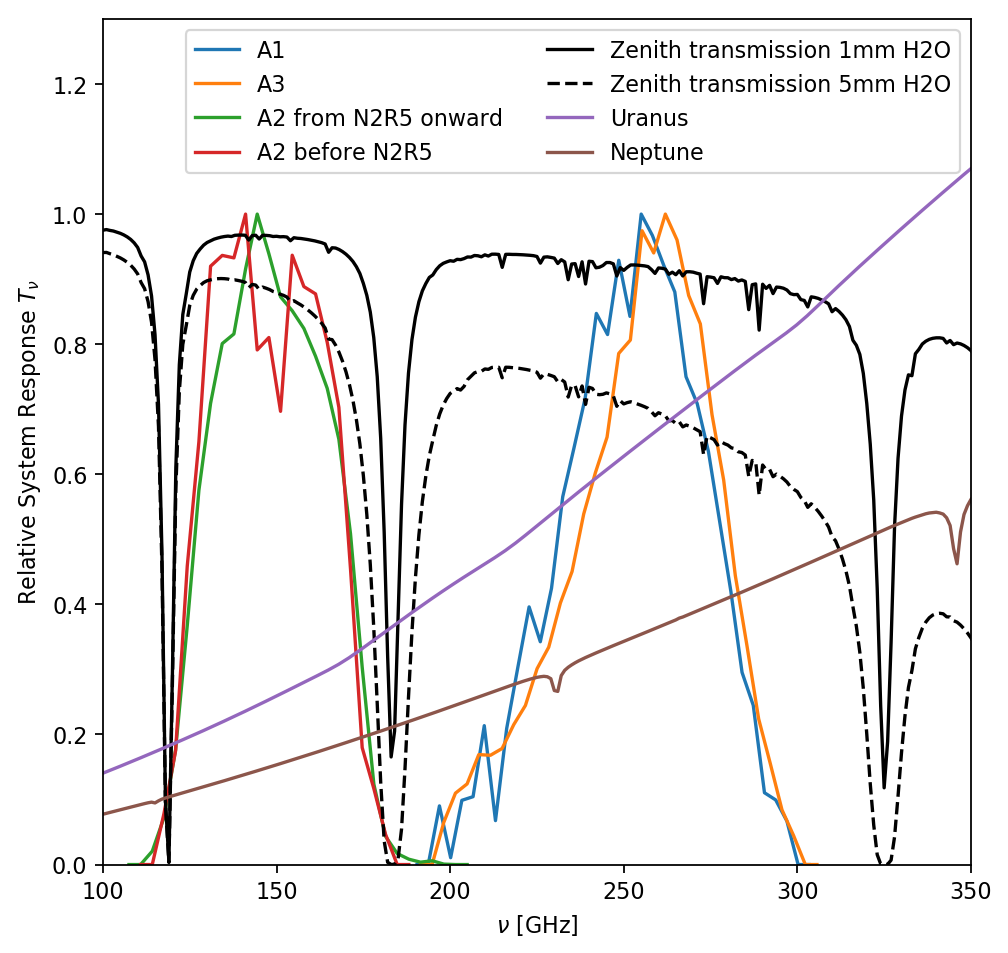
\includegraphics[width=0.75\textwidth]{Figures/SpectralBands/bandpasses_nika2.png}
\caption[NIKA2 transmission]{Relative system response of the three NIKA2 arrays as a
  function of frequency. For illustration we also plot atmospheric transmission obtained with the ATM model 
 \cite{ATM} for different values of precipitable water vapor. The spectra of ESA4 model of Uranus and ESA5 model of Neptune \cite{ESAmodel} in the frequency range are overplotted with arbitrary normalization.} 
 \label{spectralband1}
\end{center}
\end{figure}

 

The NIKA2 spectral bands were measured in the laboratory using a
Martin-Puplett interferometer built in-house \cite{durand}.  Both
arrays and filter bands were considered in the measurements. These
were obtained from the difference of two black bodies, hence they
include a $\nu^2$ Rayleigh-Jeans (RJ) spectral term.
Figure~\ref{spectralband1} shows the relative spectral response for
the three arrays (corrected of the RJ term).  Notice that array A2 was
replaced by a new one in N2R5 and that the spectral transmissions are
not the same (green and red lines in the figure).

The two arrays operating at 260 GHz, mapping different polarisations,
exhibit a slightly different spectral behaviour probably as can be
seen on figure \ref{spectralband1}. This may be explained by a tiny
difference in the silicon wafer and/or Aluminium film thicknesses. For
instance, the observed shift of the peak frequency, 265 GHz for the V
(A1) array versus 258 GHz for the H one (A3), can be explained by
about 5 microns change in the substrate thickness. Hereafter, the peak
frequencies are referred to as reference frequencies (150 and 260 GHz)
to which correspond the reference wavelengths (2.0 and 1.15 mm), see
tab.~\ref{tab:nika2summary}.


\begin{table}[th]
\begin{center}
\begin{tabular}{|l|l|r|r|r|r|r|r|}
\hline 
\multirow{3}{*}{Water vapor} & \multirow{3}{*}{Elevation} & \multicolumn{2}{|c|}{1 mm (H)} & \multicolumn{2}{|c|}{1 mm (V)} &
\multicolumn{2}{|c|}{2 mm} \\
 & & $\nu_eff$ & $\Delta \nu$  & $\nu_eff$ & $\Delta \nu$  & $\nu_eff$ & $\Delta \nu$ \\
 & & (GHz) & (GHz)  & (GHz)  & (GHz)   & (GHz)  & (GHz)  \\
\hline
\multicolumn{2}{|c|}{No atmosphere} & 254.71 & 49.21 & 257.39 & 48.05 & 150.93 & 40.72 \\
\hline
\multirow{4}{*}{1 mm $\rm H_2O$ $\rightarrow \tau_{225}=$0.067} & 90 deg &  254.46 & 48.72 & 257.12 & 47.95 & 150.93 & 39.71 \\
 & 60 deg & 254.42 & 48.68 & 257.08 & 47.93 & 150.92 & 39.60 \\
 & 40 deg & 254.33 & 48.57 & 256.98 & 47.89 & 150.88 & 39.32 \\
 & 20 deg & 254.00 & 48.21 & 256.62 & 47.77 & 150.75 & 38.45 \\
\hline
\multirow{4}{*}{2 mm $\rm H_2O$ $\rightarrow \tau_{225}=$0.120} & 90 deg &  254.26 & 48.74 & 256.91 & 48.06 & 150.64 & 39.34 \\
 & 60 deg & 254.20 & 48.70 & 256.84 & 48.07 & 150.60 & 39.19 \\
 & 40 deg & 254.02 & 48.60 & 256.65 & 48.08 & 150.48 & 38.80 \\
 & 20 deg & 253.43 & 48.30 & 256.01 & 47.93 & 150.13 & 37.62 \\
\hline
\multirow{4}{*}{3 mm $\rm H_2O$ $\rightarrow \tau_{225}=$0.173} & 90 deg &  254.06 & 48.76 & 256.70 & 48.19 & 150.39 & 39.03 \\
 & 60 deg & 253.97 & 48.73 & 256.60 & 48.21 & 150.32 & 38.84 \\
 & 40 deg & 253.71 & 48.65 & 256.33 & 48.28 & 150.14 & 38.35 \\
 & 20 deg & 252.86 & 48.41 & 255.40 & 47.86 & 149.60 & 36.94 \\
\hline
\multirow{4}{*}{5 mm $\rm H_2O$ $\rightarrow \tau_{225}=$0.278} & 90 deg &  253.67 & 48.82 & 256.28 & 48.45 & 149.96 & 38.47 \\
 & 60 deg & 253.51 & 48.81 & 256.11 & 48.44 & 149.84 & 38.22 \\
 & 40 deg & 253.10 & 48.77 & 255.68 & 48.26 & 149.54 & 37.58 \\
 & 20 deg & 251.74 & 48.67 & 254.20 & 47.75 & 148.68 & 35.82 \\
\hline
\multirow{4}{*}{8 mm $\rm H_2O$ $\rightarrow \tau_{225}=$0.437} & 90 deg &  253.08 & 48.94 & 255.66 & 48.42 & 149.38 & 37.76 \\
 & 60 deg & 252.84 & 48.93 & 255.39 & 48.35 & 149.20 & 37.42 \\
 & 40 deg & 252.21 & 48.94 & 254.71 & 48.16 & 148.77 & 36.64 \\
 & 20 deg & 250.12 & 49.38 & 252.43 & 47.91 & 147.52 & 34.57 \\
\hline
\multirow{4}{*}{10 mm $\rm H_2O$ $\rightarrow \tau_{225}=$0.542} & 90 deg &  252.70 & 49.00 & 255.24 & 48.38 & 149.04 & 37.34 \\
 & 60 deg & 252.39 & 49.01 & 254.92 & 48.29 & 148.82 & 36.97 \\
 & 40 deg & 251.62 & 49.11 & 254.08 & 48.13 & 148.31 & 36.12 \\
 & 20 deg & 249.07 & 49.75 & 251.28 & 48.24 & 146.85 & 33.93 \\
\hline
\end{tabular}
\caption[Effective frequencies and bandwidthes]{Effective frequencies (for Uranus) and bandwidth of the NIKA2 bands for
  various atmospheric conditions and elevation.}
\label{tab:bandwidths}
\end{center}
\end{table}

%What actually matters more than the ``central frequency'' that depends on many
%assumptions and definitions are the bandpasses. We should make available in a
%.fits file, clearly, our bandpasses to avoid future misunderstanding and propagation of
%false numbers. Official values should be 150 and 260~GHz. We should also clearly
%state that these measured bandpasses were done with the difference of two
%black-bodies, hence they include a $\nu^2$ RJ term.\\

{\color{red} LP: to be moved to Section Calibration ? Opacity ? }


The total system response is the multiplication of the atmospheric
transmission with the relative system response. To derive the
atmospheric transmission, we use GILDAS ATM 2009 model \cite{ATM}, computed for
the IRAM 30-m telescope, with so called {\it midlatwinter} conditions. We select in the model
grid an atmosphere with $T=268.3 \ {\rm K}$ and a pressure of $703.5 \ {\rm hPa}$. The
effective frequency of the passband is defined by:
\begin{equation}
\nu_{eff}( \sec \delta, mm_{H_{2}O}) = \frac{ \int_{0}^{+\infty} S_{\nu}
  T_{\nu}(\sec \delta, mm_{H_{2}O}) \nu d\nu } { \int_{0}^{+\infty} S_{\nu} T_{\nu} d\nu}
\label{eq:nueff0}
\end{equation}

{\color{blue} FXD: we should integrate over SOmega (nu-2). For
  MartinPuplett measurements, the source spectrum was RJ (nu2) so that
  cancels out to find Tnu. Snu is for an extended source. Deltanu
  should be with respect to a spectrum, for example RJ. I think the
  table 2.1 is not very useful. It could be a figure (nueff as a
  function of tauLOS (elevation is not relevant)? or just few numbers:
  we should at the end state what is nueff and deltanu for average
  conditions. Nomenclature: 1mm(H) is not the usual denomination... }


where $T_{\nu}$ is the total system response, normalized between
0. and 1. (i.e. a relative response as a function of the frequency),
hereafter referred to as RSR (Relative System Response), $S_{\nu}$ is
the source spectrum. Table~\ref{tab:bandwidths} lists this effective frequency,
computed for Uranus spectrum (ESA4 model, \cite{ESAmodel}), for different atmospheric
water vapor contents and different elevations. 
Table~\ref{tab:bandwidths} also list the bandwidth, defined as:
\begin{equation}
\Delta\nu = \int_{0}^{+\infty} \frac{T_{\nu}}{Max(T_{\nu})}
d\nu
\end{equation}
where the $Max(T_{\nu})$ ensure the RSR span the whole 0.0 to 1.0 range.

From Table~\ref{tab:bandwidths}, we see that the 2 mm band is somewhat
sensitive to the atmospheric conditions, especially at low
elevation. Note that these effective frequencies are {\em not} the
reference frequencies for the band, respectively 150 GHz and 260 GHz
for the A2 and A1, A3 arrays. These reference frequencies are chosen
as round numbers in the middle of the bands to define NIKA2
photometric system as will be discussed in section~\ref{se:cal_HA}.

%
% LP: the paragraph below rather belongs to the Opacity section
%
%Using the NIKA2 bandpasses for N2R9, we can integrate the ATM
%atmospheric model to compute the expected ratio between the
%atmospheric opacity of the two NIKA2 channels. 
%Figure~\ref{thopacities} shows the atmospheric opacity
%ratio of the 2 and 1 mm channels as a function of the opacity for the
%1 mm one.

%\begin{figure}[ht] % Inline image example
%\begin{center}
%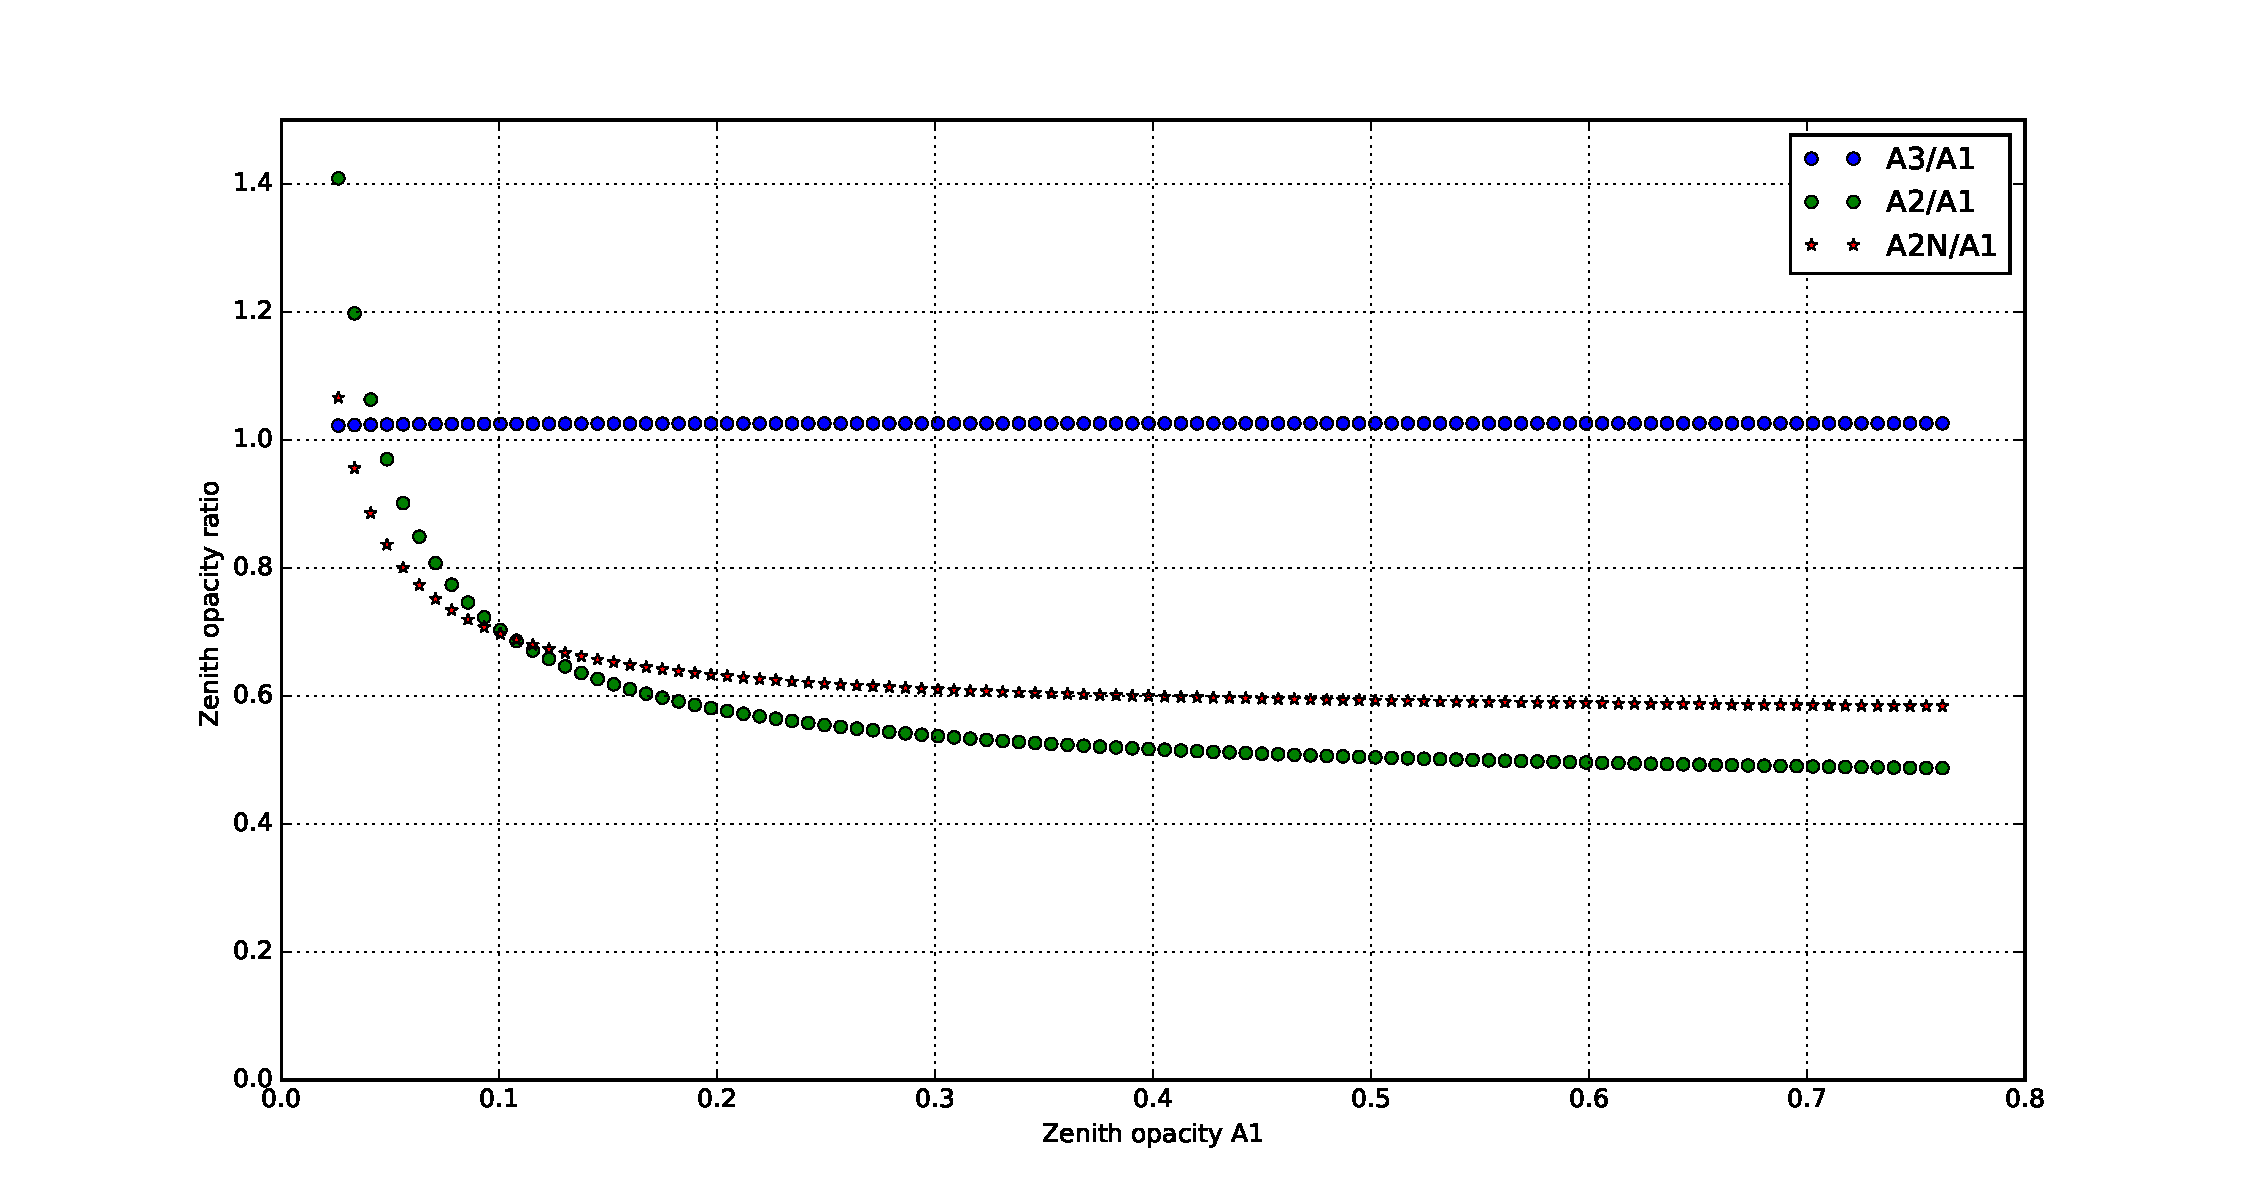
\includegraphics[width=\textwidth]{Figures/SpectralBands/opacity_ratio_vs_tau1.pdf}
%\caption{Expected atmospheric opacity ratio of the 2 and 1 mm channels as function 
%of the opacity at 1 mm. {\bf FM: what is A2N/A1 ?} {\bf FM: why is A3/A1=1 ?}}
%\label{thopacities}
%\end{center}
%\end{figure}





%-------------------------

\subsection{Cryogenics}

The optimal operation of the detectors is achieved at a temperature of around
150\,mK, well below the Aluminium superconducting transition. For this reason,
NIKA2 employs a custom dilution fridge to cool down the focal plane, and the
refractive portion of the optics, for a total mass around 100 kg, deeply in the
sub-Kelvin regime. Despite the complexity and size of the system, the operation
of NIKA2 does not require external cryogenic liquids and is fully remotely
controllable.

\subsection{KIDs and electronics}
\label{se:array}

The 150\,GHz channel is equipped with A2 that is an array of
616\,pixels, arranged to cover a 78\,mm diameter circle. Each pixel has a size of
$2.8\times2.8\textrm{\,mm}^2$. The array A2 is connected over four different
readout lines. In the case of the 260\,GHz band detectors, the pixel size is
$2\times 2\mathrm{\,mm}^2$, to ensure a comparable sampling of the focal
plane. In order to fill the two 260\,GHz arrays A1 and A3, a total of 1,140 pixels are
needed in each of them. The focal planes are all based on thin Aluminium films
deposited by e-beam evaporation under ultra-high vacuum conditions over a
Silicon substrate.

The key advantage of the KID technology is the simplicity of the cold
electronics and the multiplexing scheme. In NIKA2, each block of around 150
detectors is connected to single coaxial line providing the excitation and the
readout at the two ends. Each of the readout lines is linked to the input of a
cryogenic (4 K) low-noise amplifier. The warm electronics required to digitize
and process the pixels signals is composed of twenty custom readout cards (one
per feed-line).

%In this document, the 2\,mm array is called A2, while the two 1\,mm arrays are
%called A1 and A3.


\subsection{KID photometry and tuning}

\begin{figure}[!b]
\begin{center}
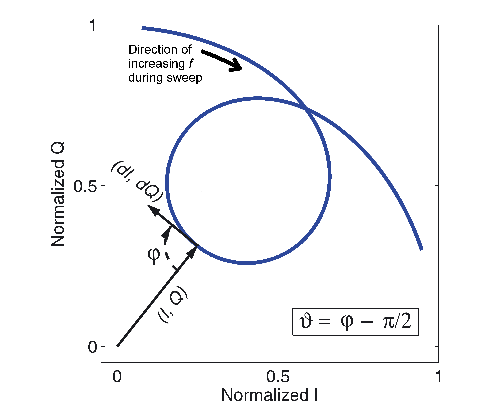
\includegraphics[width = 0.7\textwidth]{Figures/resoCircle-eps-converted-to.pdf}
\caption[KID resonance circle]{Sample resonance circle in the IQ plane. Both the
  tuning procedures are based on the measurement of the angle $\vartheta$
  between the two vectors ($I, Q$) and ($dI, dQ$)}
\label{figResoCircle}
\end{center}
\end{figure}

Kinetic Inductance Detectors are superconducting resonators whose resonance
frequency shifts linearly depending on the incoming optical power. The measure of such
frequency shift $\Delta f$ is what allows us to use KID as mm-wave detectors.

For the KID readout, an excitation signal is sent into the cryostat on the
feedline coupled to the KID. The transmitted signal can be described by its
amplitude and phase, or, as is common practice for KID, by its components that
are In-phase ($I$) and in Quadrature $Q$ with respect to the excitation
signal. When a frequency sweep is carried around a KID resonance, the
transmitted signal makes a sort of circle in the $I-Q$ plane, as shown
in Fig.~\ref{figResoCircle}.
The goal is now to relate the variations $(\Delta I, \Delta
Q)$ along this circle induced by incident light to the $\Delta f$. For this, the
electronics modulates the excitation frequency at about 1\,kHz with a known
$\delta f$ frequency variation and the read out gives the induced $(dI,
dQ)$. Projecting linearly $(\Delta I, \Delta Q)$ on $(dI, dQ)$ therefore
provides $\Delta f$. This value, in Hz, is the raw input timeline to the
pipeline and will be futher calibrated into astronomical units
(sect.~\ref{se:calibration}). For historical reasons, this way of deriving KID
signals has been nicknamed \emph{RfdIdQ}. More details on this process are given
in \cite{Calvo13}.\\

Not only incident astronomical light reaches the KIDs and contributes to Cooper
pair breaking. Any change in the background optical load (due, for example, to changes in
the atmospheric transmission or in the elevation) contributes as well to the
shift of the resonances. In order to maximize the sensitivity of a KID, the
excitation signal used to read it out must always be near its resonance
frequency. We therefore have developped a tuning algorithm that takes care of
this optimization. Tunings are performed during the first subscan of each
observation in order to be optimally tuned at the same elevation and sky
conditions as the source. It takes only a few seconds when the $f_{tones}$ are
close to the current functionning point. In order to always be in these
conditions, continuous tunings are done between two scans when NIKA2 is not observing.

A specific case is when we do {\tt skydips}. In this case, we tune all the KIDS
at the beginning of each subscan/elevation step on purpose to monitor the
induced variation of $f_{tone}$ by the sky load.


%% Data reduction: explain what is needed to go from raw timelines to maps.
%% it will be a list of what is needed with very little description that will
%% announce the details on each item that is developped in the following
%% sections.


\section{Overview of the data reduction pipeline}% {\color{YellowGreen} Nico}}
\label{se:pipeline_overview}

Because each matrix of \nika\ is a filled array with more than one
detector per \new{main beam} PSF on average, and because the atmosphere and electronic noise act as
correlated low frequency parasites, the data reduction of \nika\ does not
proceed on an individual KID basis in general. This, in addition to the
necessary pointing information specifies some of the data reduction
process. In short, the data reduction proceeds as such:

\begin{itemize}
\item Low level processing (Sect.~\ref{se:ll_proc})
\item Pointing reconstruction (Sect.~\ref{se:ptg})
\item TOI calibration and opacity correction (Sect.~\ref{se:flux_calib})
\item TOI processing (Sect.~\ref{se:toi_proc})
\item Map projection (Sect.~\ref{se:map_projection})
\item Photometry (Sect.~\ref{se:intro_photometry})
\end{itemize}

\subsection{Low level processing}
\label{se:ll_proc}

A first step of the analysis is to read the data produced by \nika's
acquisition. The data as such comprise various quantities that describe the
variations of the KID's resonance frequencies, such as $I$, $Q$, $dI$,
$dQ$. From these quantities, and throughout this work, we use our so called
\rf\ photometric estimator that combines them into a quantity that is
proportionnal to the flux absorbed by a KID \cite{Calvo13} and homogeneous to Hz.

In addition to this, we look for and remove the - rare - cosmic rays
events. KIDs have such fast time constants that unlike bolometers, these events
affect a sole sample that is easy to detect by a simple comparison to the rms of
the TOI a few second window. These affected samples are remplaced by a simple
linear interpolation of their surrounding (not to leave holes in the TOI) but
are flagged in order not to project false data on the final map.

We also have a series of tests that read flags from the acquisition
overall. These flags monitor potential jumps in the cryostat or acquisition
monitoring. Most important are the flags related to the tuning. Because the
acquisition file boundaries are not strictly linked to the beginning and the end of
a scan, we must discard everything that happens before the last tuning of the
beginning, and everything after the first automatic tuning that happens when the
scan is done.

Because the tuning of KIDs might fail from time to time depending on the weather
conditions for instance, we systematically check each KID and see if its noise
is far from the average noise of all other KIDs in the same array, with a
typical $3\,\sigma$ threshold. This criterion may seem a bit tight, but in any case, KIDs
are inverse noise variance weighted in the final map projection, so they would
be given relatively low weight anyway (see Sect.~\ref{se:map_projection}).

At this stage of the processing, we have isolated the relevant fraction of the
data for scientific processing and flagged out potentially misbehaving KIDs or
timeline accidents (glitches).

\subsection{Pointing reconstruction}
\label{se:ptg}

This step consists in addressing each sample of each KID to the correct sky
coordinates and their associated map pixel. The pointing data\sam{, as
produced by the control system of the telescope, \aka\ NCS, } are passed to the
\nika\ raw data. They describe the absolute
pointing of a reference point in the focal plane in various quantities, the
absolute azimuth and elevation $(\alpha,\delta)$ of the source, together with
offsets $(\Delta\alpha_t, \Delta\delta_t)$ \wrt~these. Because our final maps
will be centered on a fixed position (typically the center of the source that is
aimed by the focal plane reference position), we are especially interested in
pointing offsets \wrt~this position. We therefore detail here the derivation of
these offsets.

We store KID pointing offsets \wrt\ the reference position in Nasmyth $(x,y)$
coordinates (independent of time) once and for all in our KID database
(\aka~\kidpar). Sect.~\ref{se:fp_reconstruction} details how these offsets are
derived. To go from Nasmyth offsets to $(\alpha,\delta)$ offsets, we apply the
following rotation by the elevation angle:

\begin{eqnarray}
\Delta\alpha^k_t &=&  \cos\delta_t \Delta x^k + \sin\delta_t \Delta y^k, \nonumber\\
\Delta\delta^k_t &=& -\sin\delta_t \Delta x^k + \cos\delta_t \Delta y^k, \nonumber
\end{eqnarray}

where $k$ is a KID index. Adding these offsets to the reference $(\Delta
\alpha_t, \Delta \delta_t)$ gives the absolute pointing of each KID in these
coordinates. An extra rotation by the parallactic angle $\eta_t$ is required to
obtain KID's coordinates in \radec\ coordinates:

\begin{eqnarray}
\Delta R.\,A.^k_t &=&  \cos\eta_t \Delta\alpha^k_t + \sin\eta_t \Delta\delta^k_t,\\
\Delta Dec^k_t    &=& -\sin\eta_t \Delta\alpha^k_t + \cos\eta_t \Delta\delta^k_t.
\end{eqnarray}

We now have the pointing of each KID at each time relative to the source that we
usually center on our final map. It is then trivial to assign the map pixel
corresponding to this pointing on a Nearest Grid Point basis.

This pointing reconstruction is done early in the data reduction process because
we'll need to know when a KID is close or far from the source for the timeline
processing (Sect.~\ref{se:toi_proc}).

\subsection{TOI calibration}
\label{se:flux_calib}

We now focus on the absolute calibration of each TOI. As stated in
Sect.~\ref{se:ll_proc}, at this stage of the reduction each KID \rf~timeline is
in Hz. The conversion process to go from these Hz into Jy/beam proceeds in two
steps: a standard absolute calibration and a correction for the current opacity
and elevation.

The standard conversion from Hz to Jy/beam is stored in the
\kidpar\ database. The derivation of these gains $g(k)$ is detailed in
Sect.~\ref{se:fp_reconstruction}. Suffice is to say here that simply multiplying
the TOI's by these gains converts them into Jy/beam. Of course, this individual
absolute calibration also acts as a relative calibration. This calibration is
meant to work at zero opacity and 90$^\circ$ elevation. We thus need to correct
for the current opacity $\tau$ and elevation. In short, the absolute calibration reads

\begin{equation}
TOI^k(t) [{\rm Jy/beam}] = \rf^k(t)[{\rm Hz}] \times g(k) \times e^{\tau_t/\sin\delta_t}
\end{equation}

The derivation of opacity is presented in Sect.~\ref{se:opacities}.

\subsection{TOI processing}
\label{se:toi_proc}

\begin{figure}[ht!]
\begin{center}
\includegraphics[clip, angle=0, scale=0.4]{Figures/toi_plot.eps}
\includegraphics[clip, angle=0, scale=0.4]{Figures/toi_plot_decorr.eps}
\caption[Example of Time-Ordered-Information]{\emph{Left:} Example of 40 KID raw timelines during an observation
  of Uranus. The low frequency correlated component (atmosphere and electronic
  noise) is clearly seen. \emph{Right:} One of these TOIs and the scaled
  \cm\ that is subtracted from it.}
\label{fig:nika_toi}
\end{center}
\end{figure}

\begin{figure}[ht!] 
\begin{center}
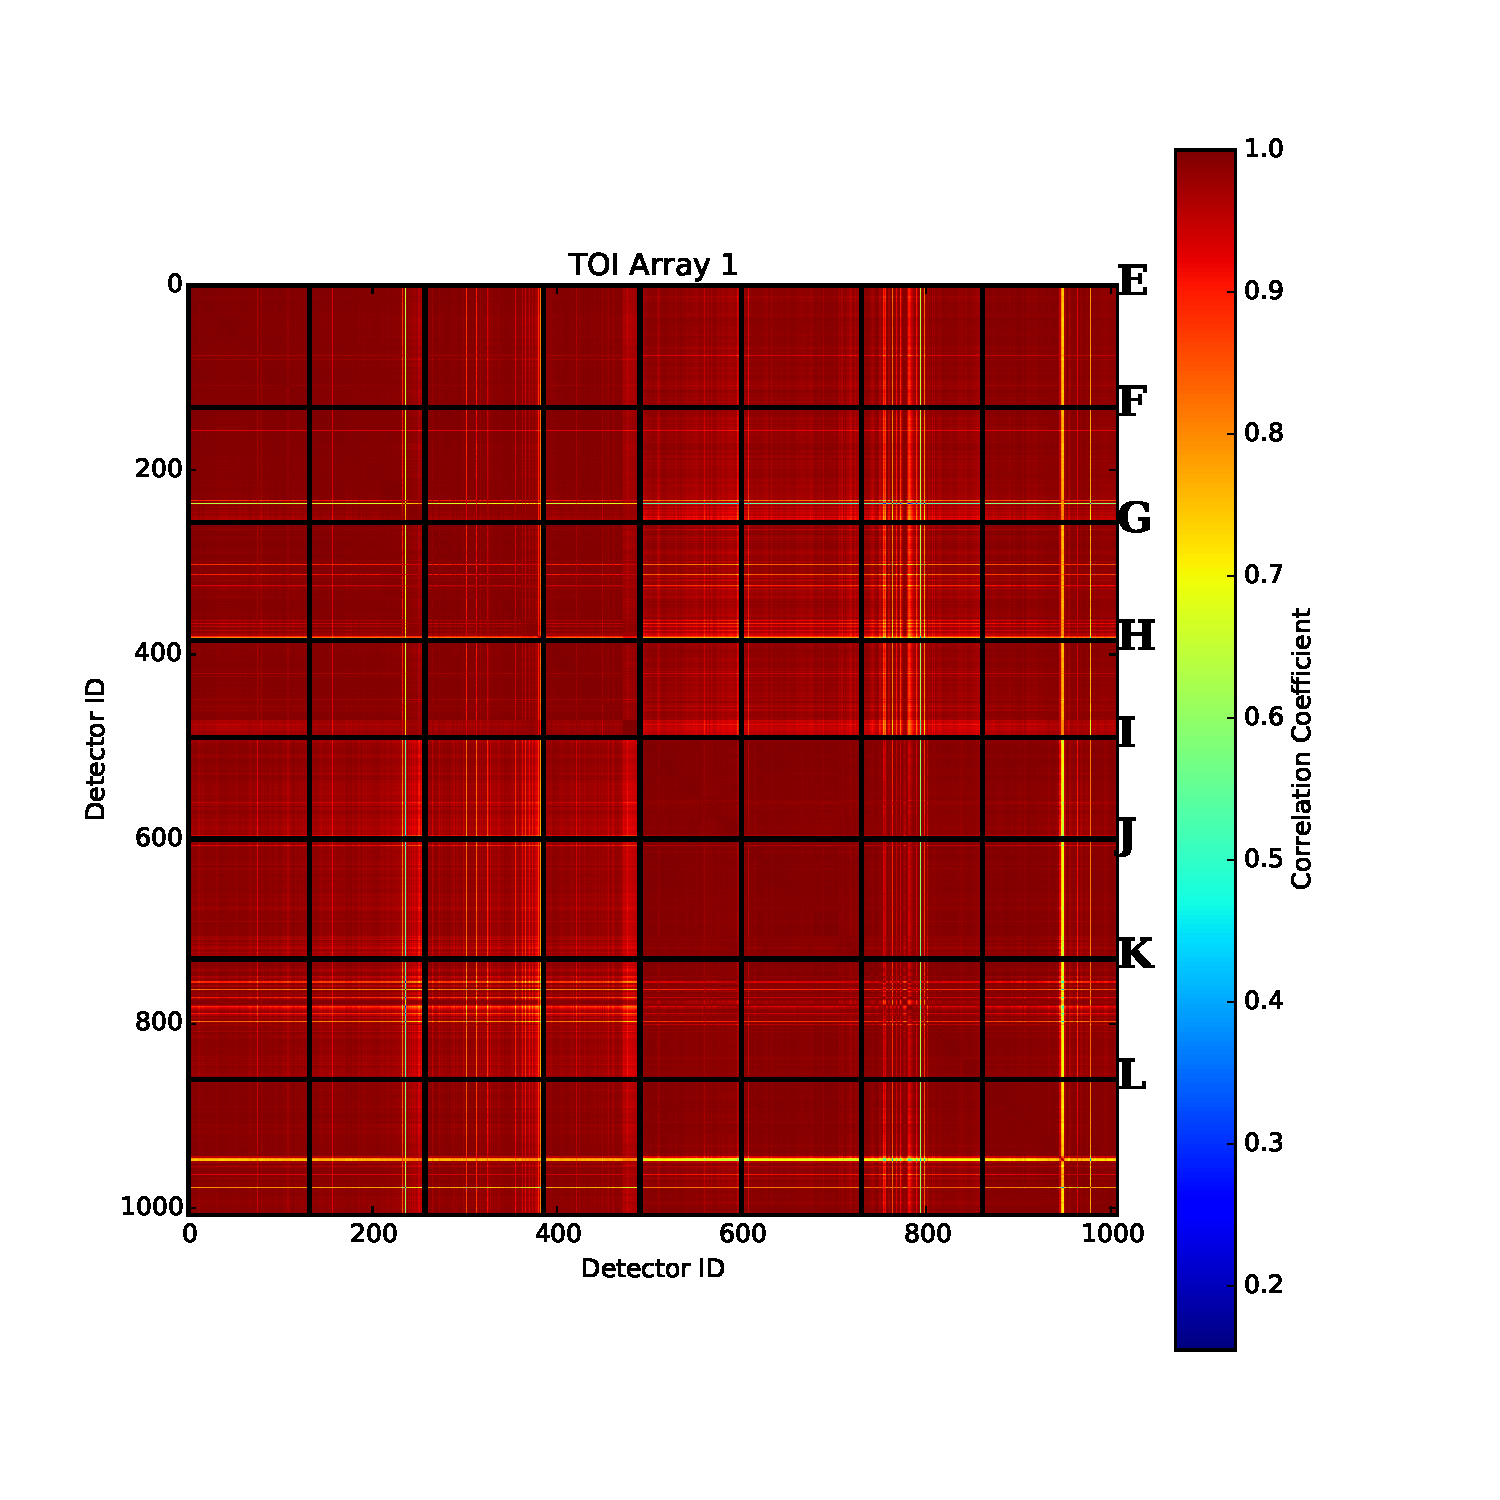
\includegraphics[width=0.3\textwidth]{Figures/NoiseTests/corrmat_TOI_array_1_20170228s151.pdf}
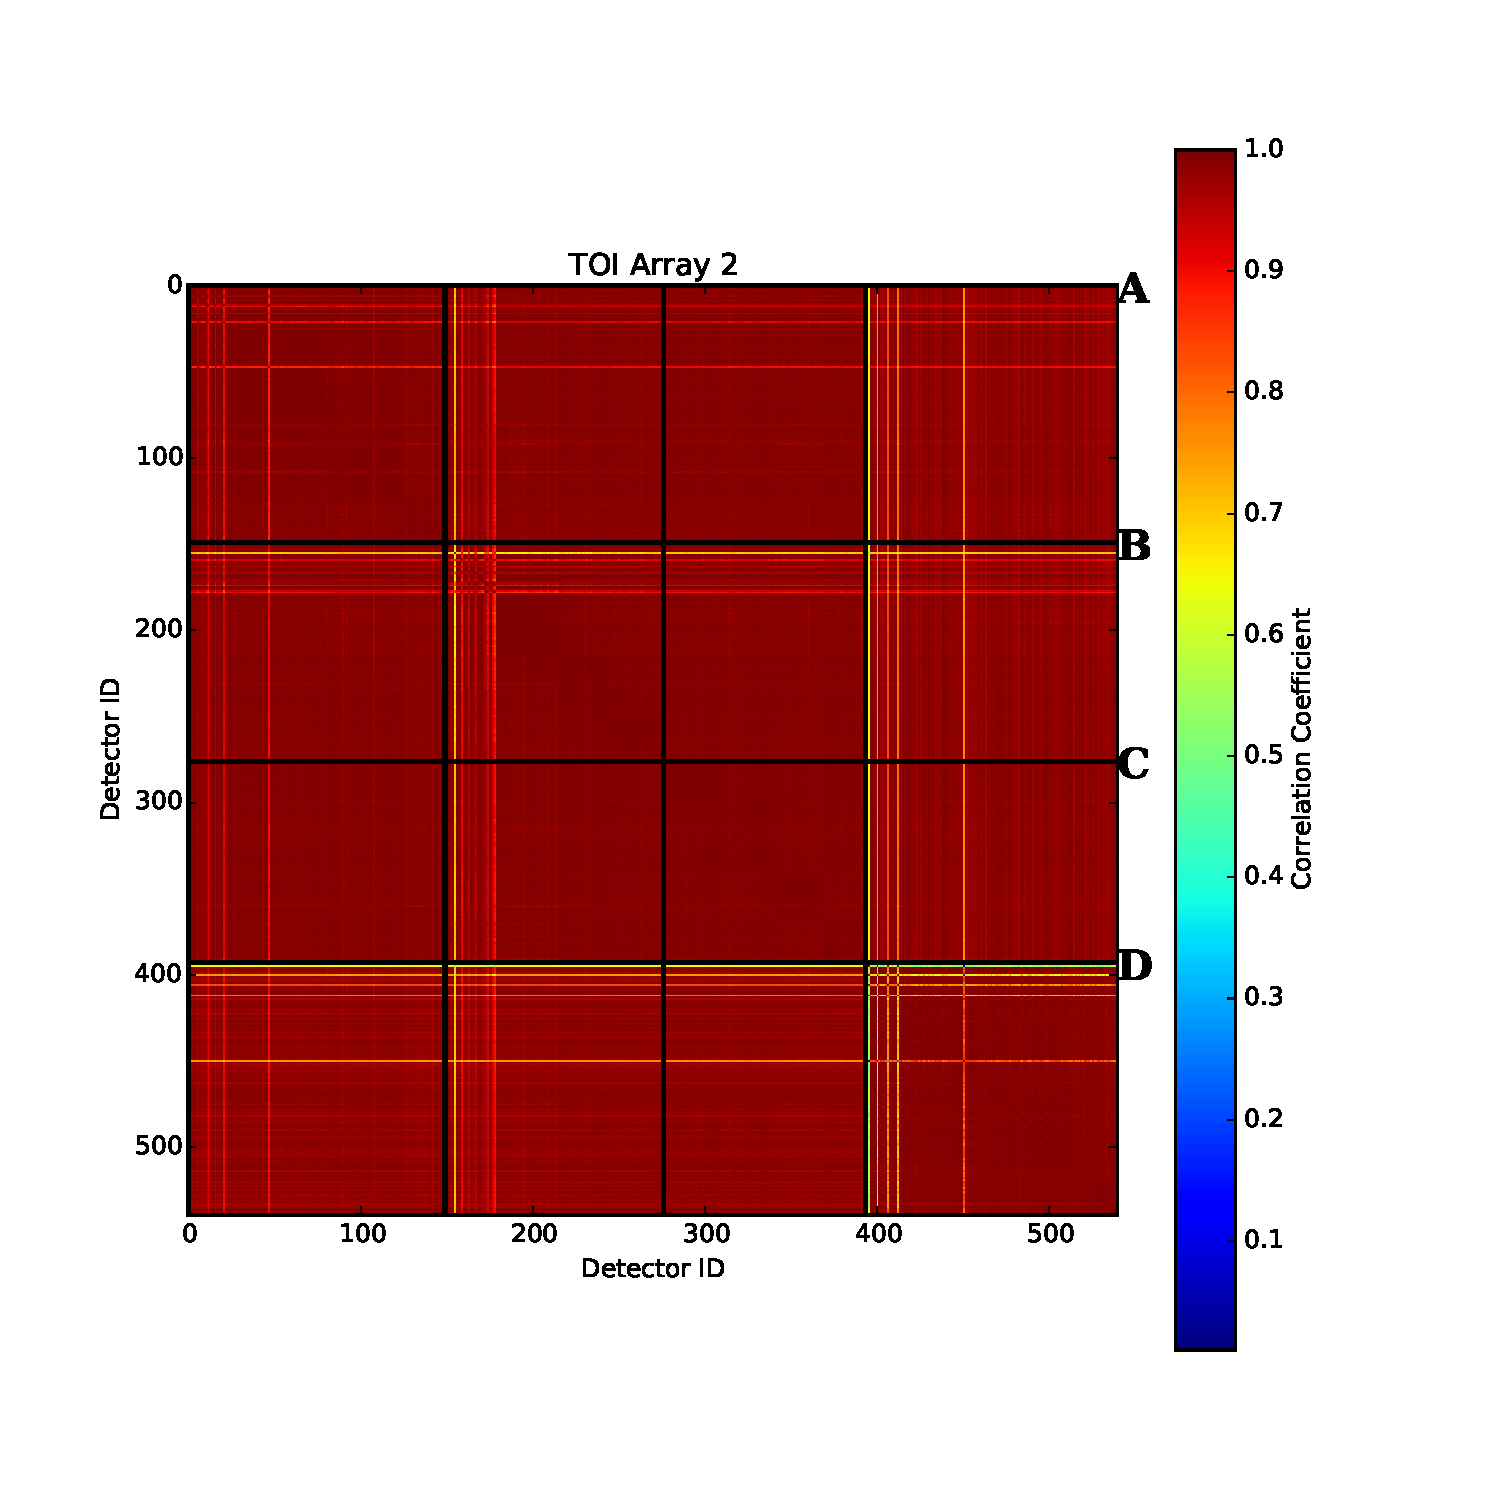
\includegraphics[width=0.3\textwidth]{Figures/NoiseTests/corrmat_TOI_array_2_20170228s151.pdf}
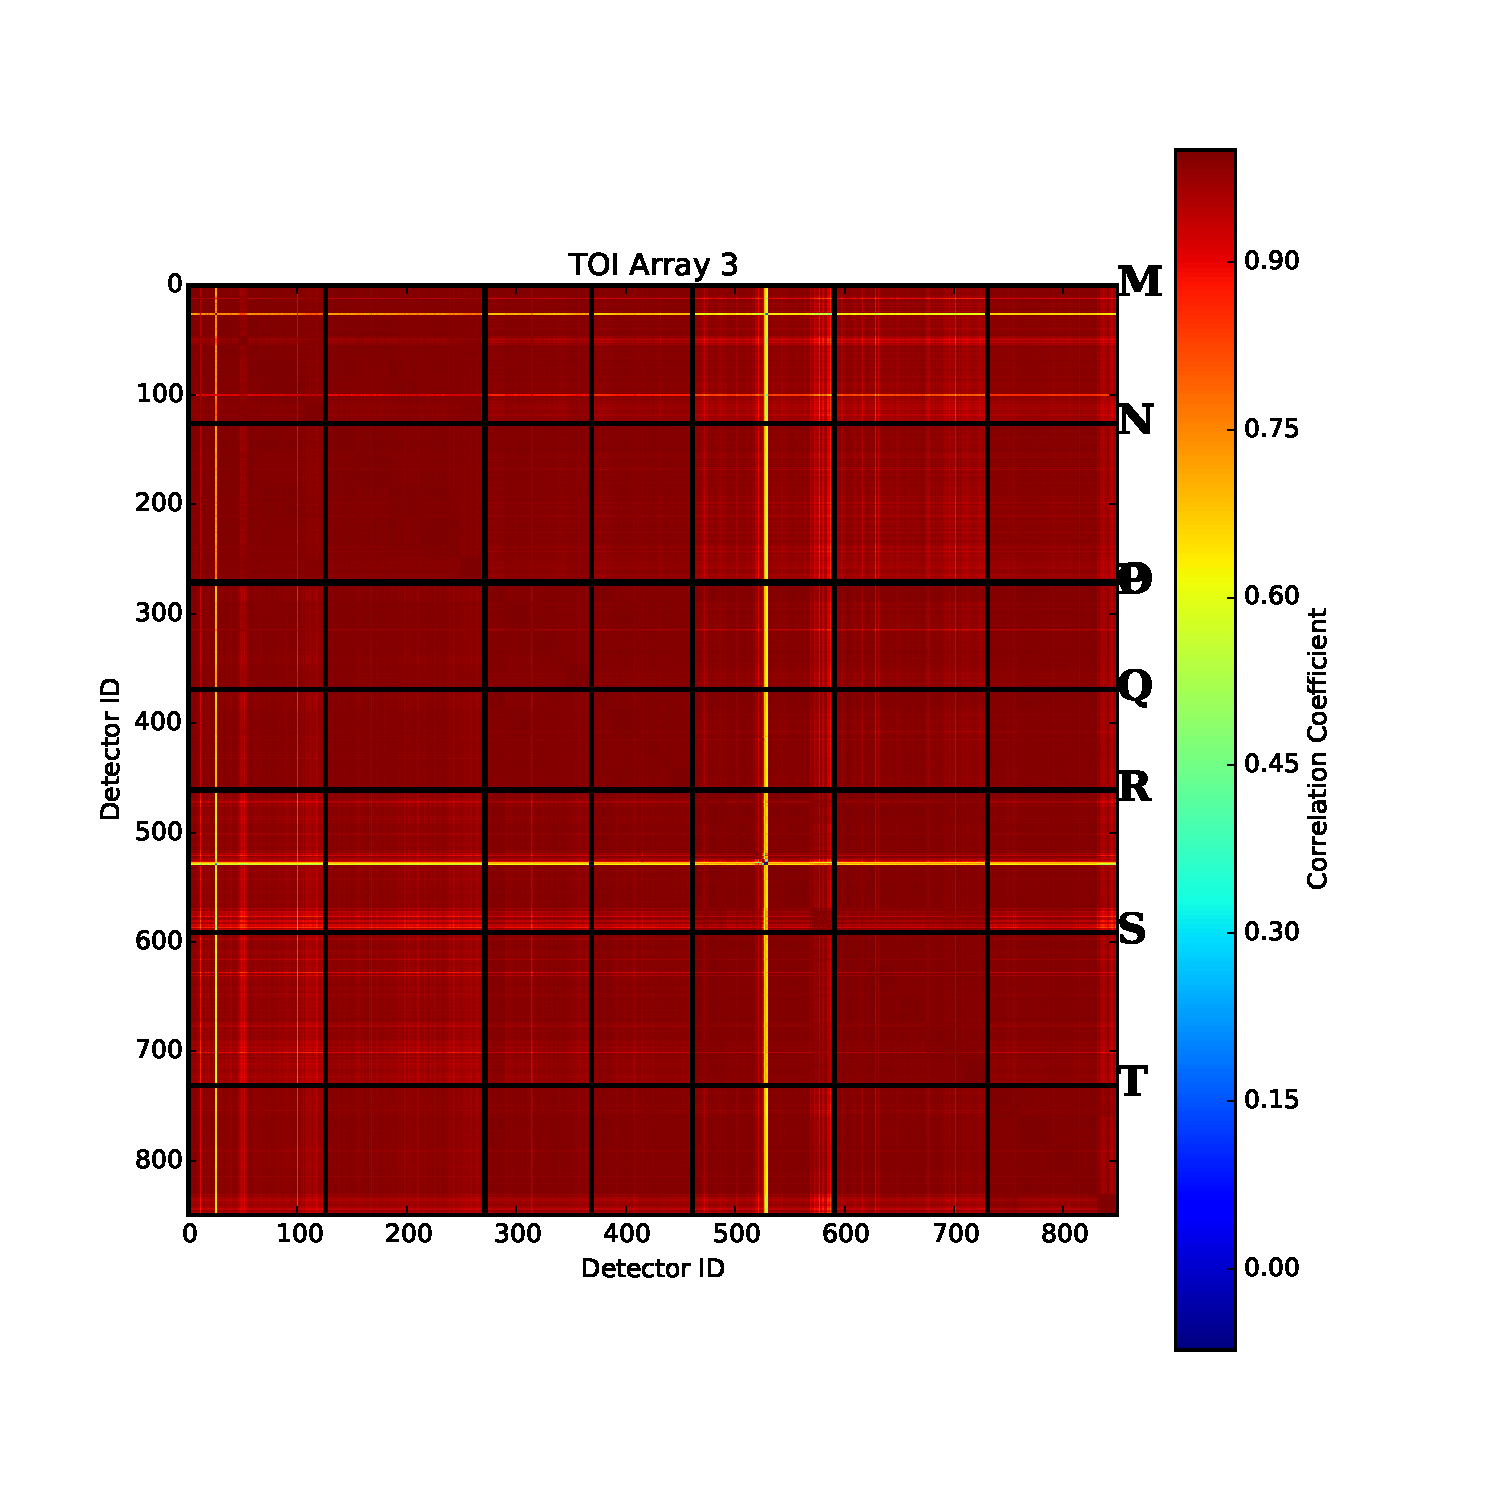
\includegraphics[width=0.3\textwidth]{Figures/NoiseTests/corrmat_TOI_array_3_20170228s151.pdf}
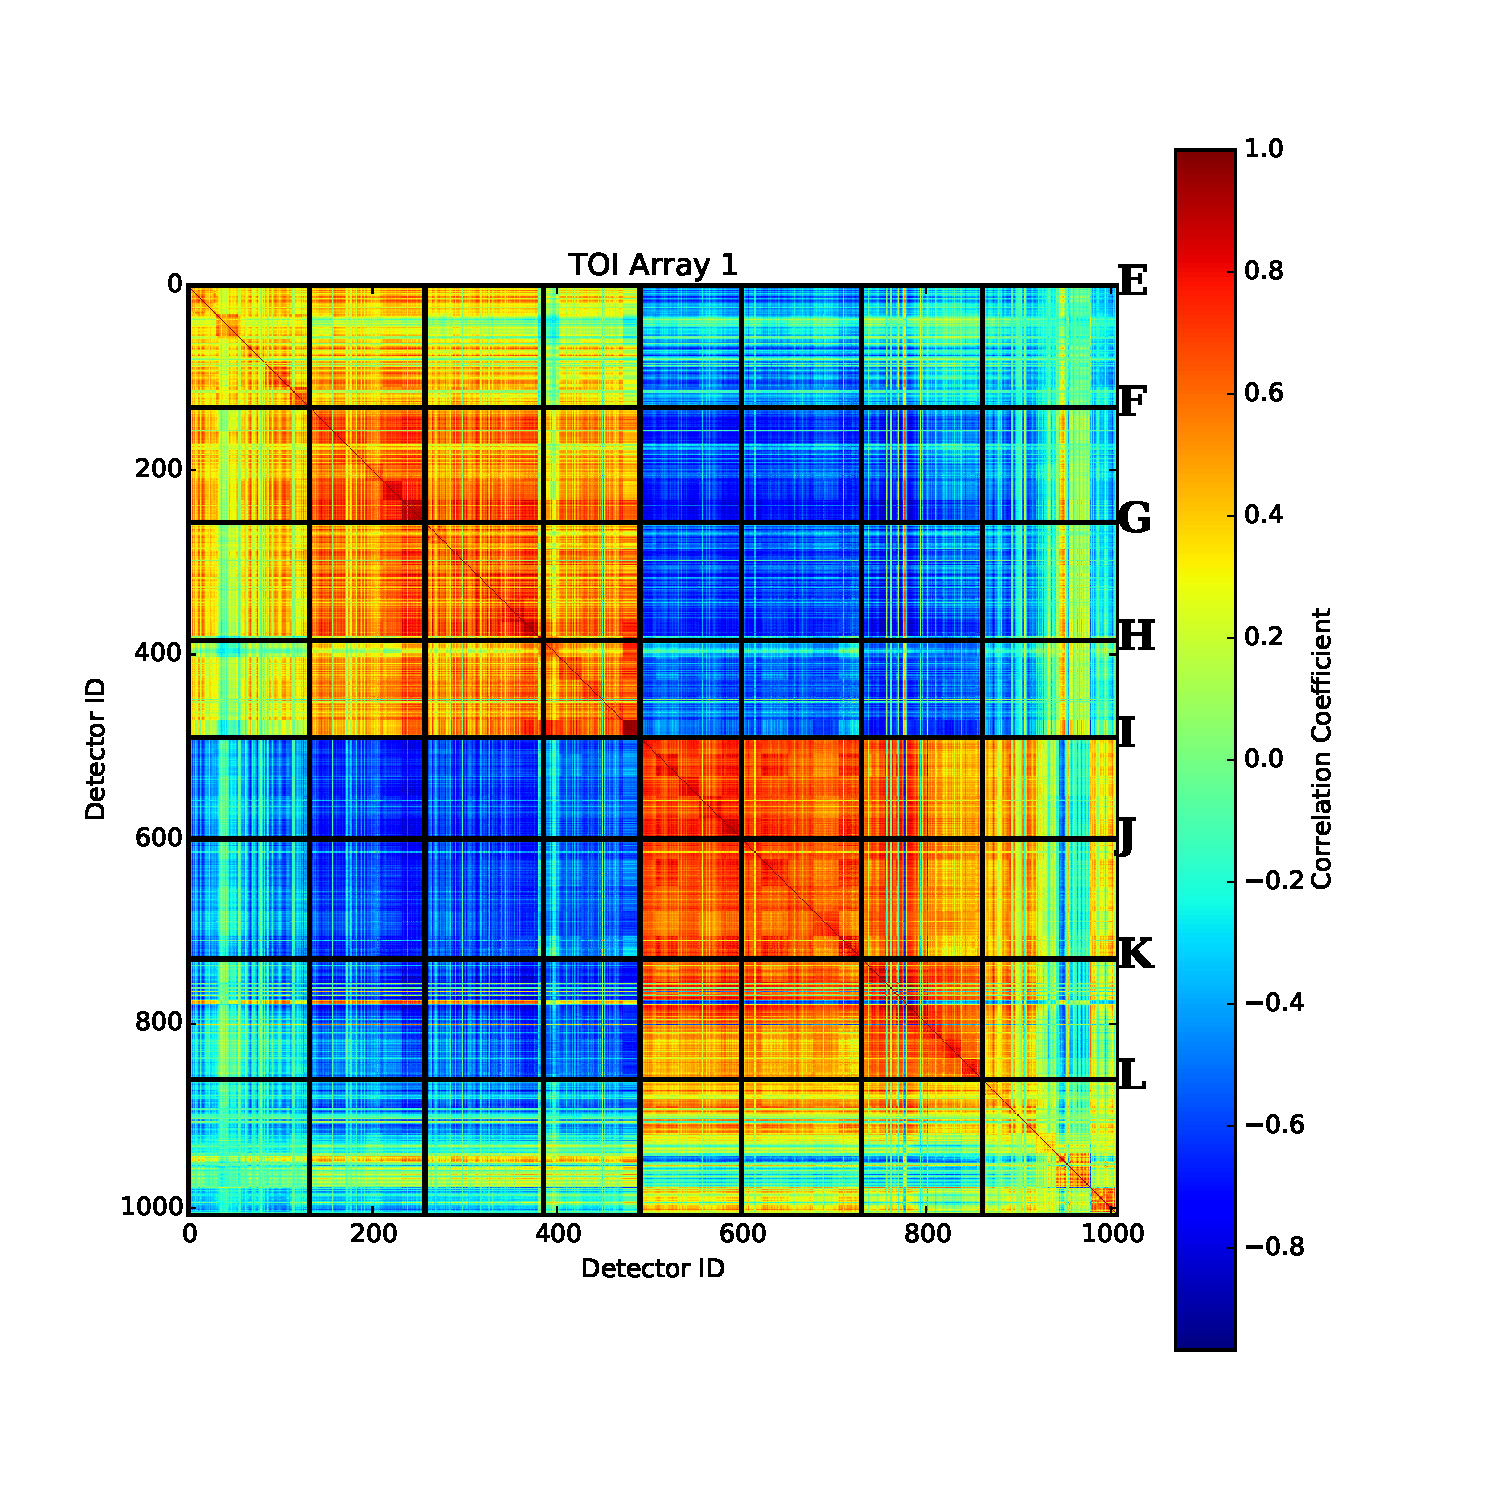
\includegraphics[width=0.3\textwidth]{Figures/NoiseTests/corrmat_TOI_CM_array_1_20170228s151.pdf}
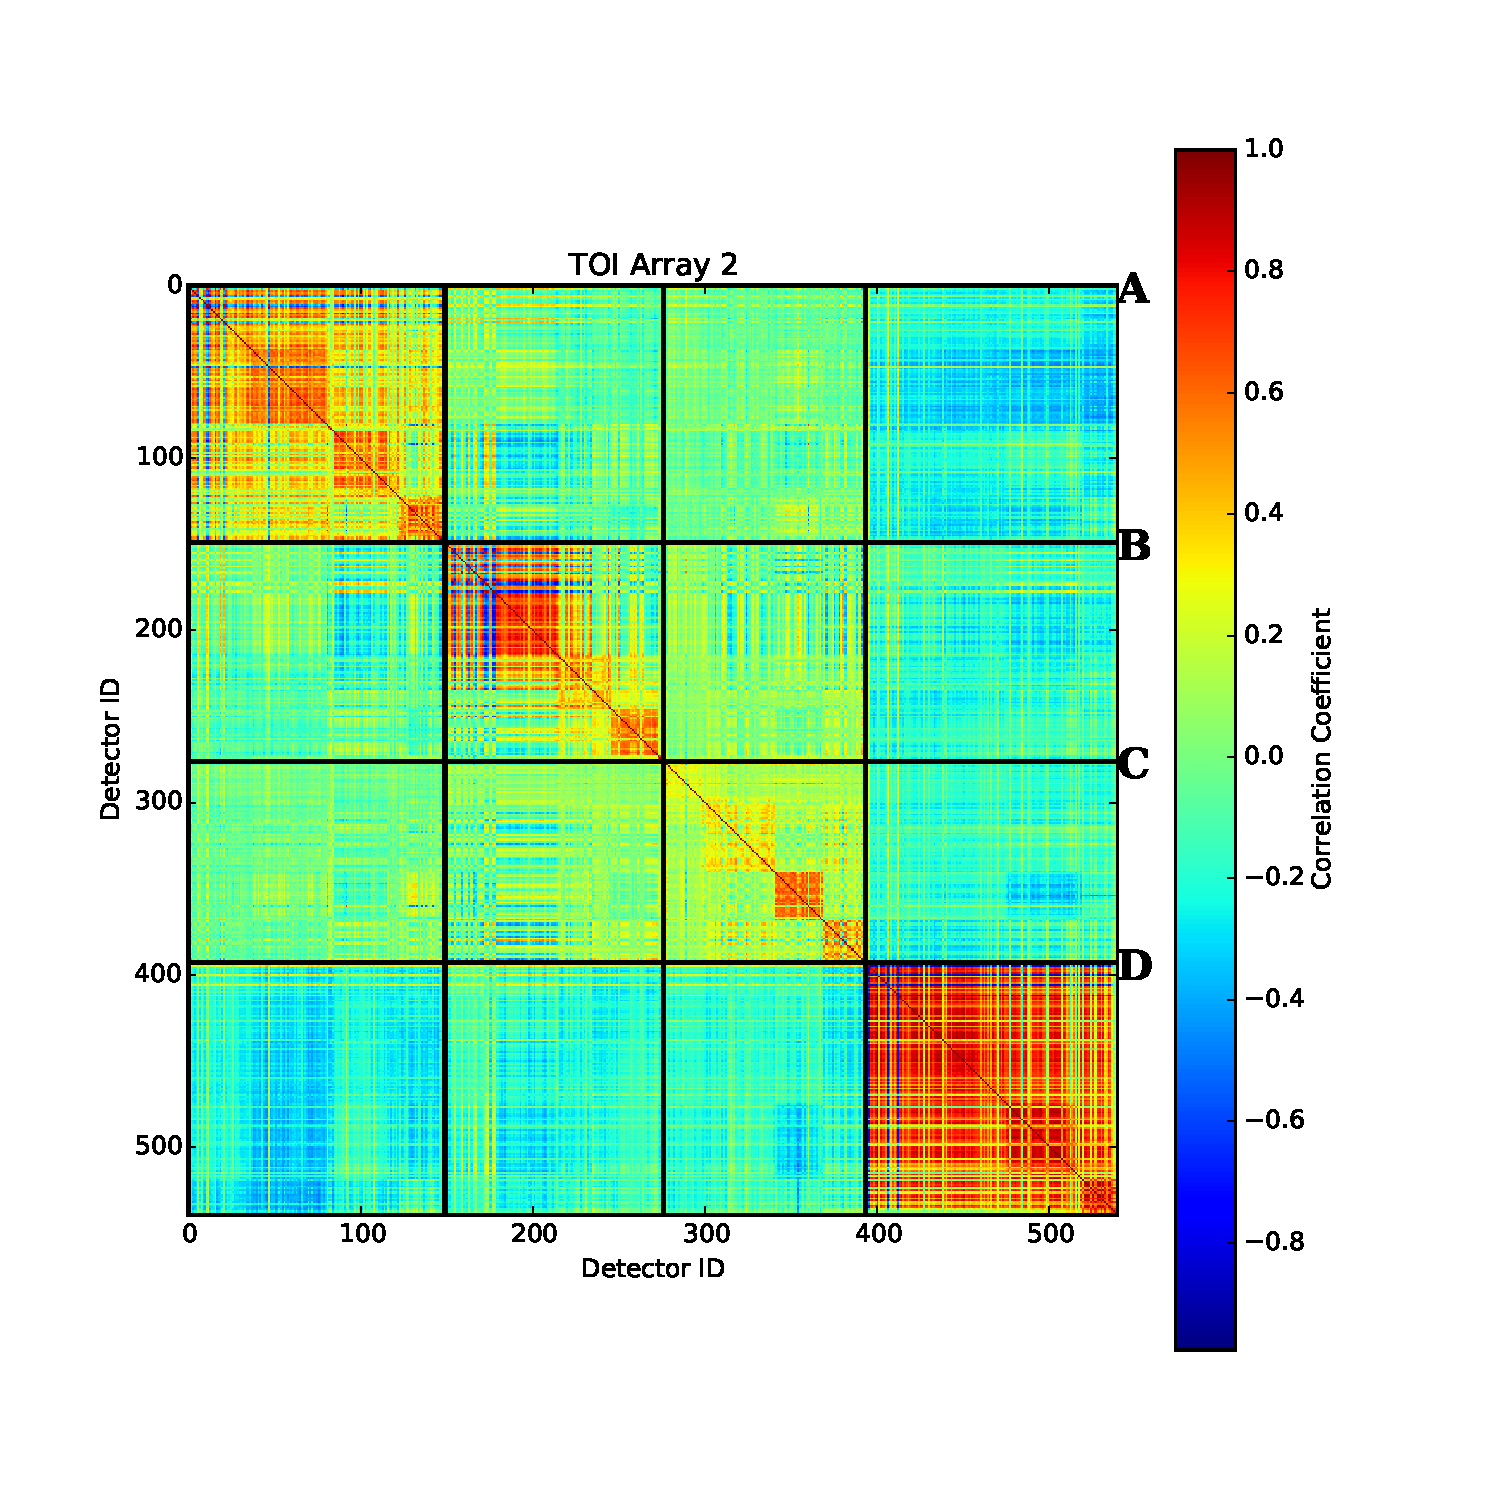
\includegraphics[width=0.3\textwidth]{Figures/NoiseTests/corrmat_TOI_CM_array_2_20170228s151.pdf}
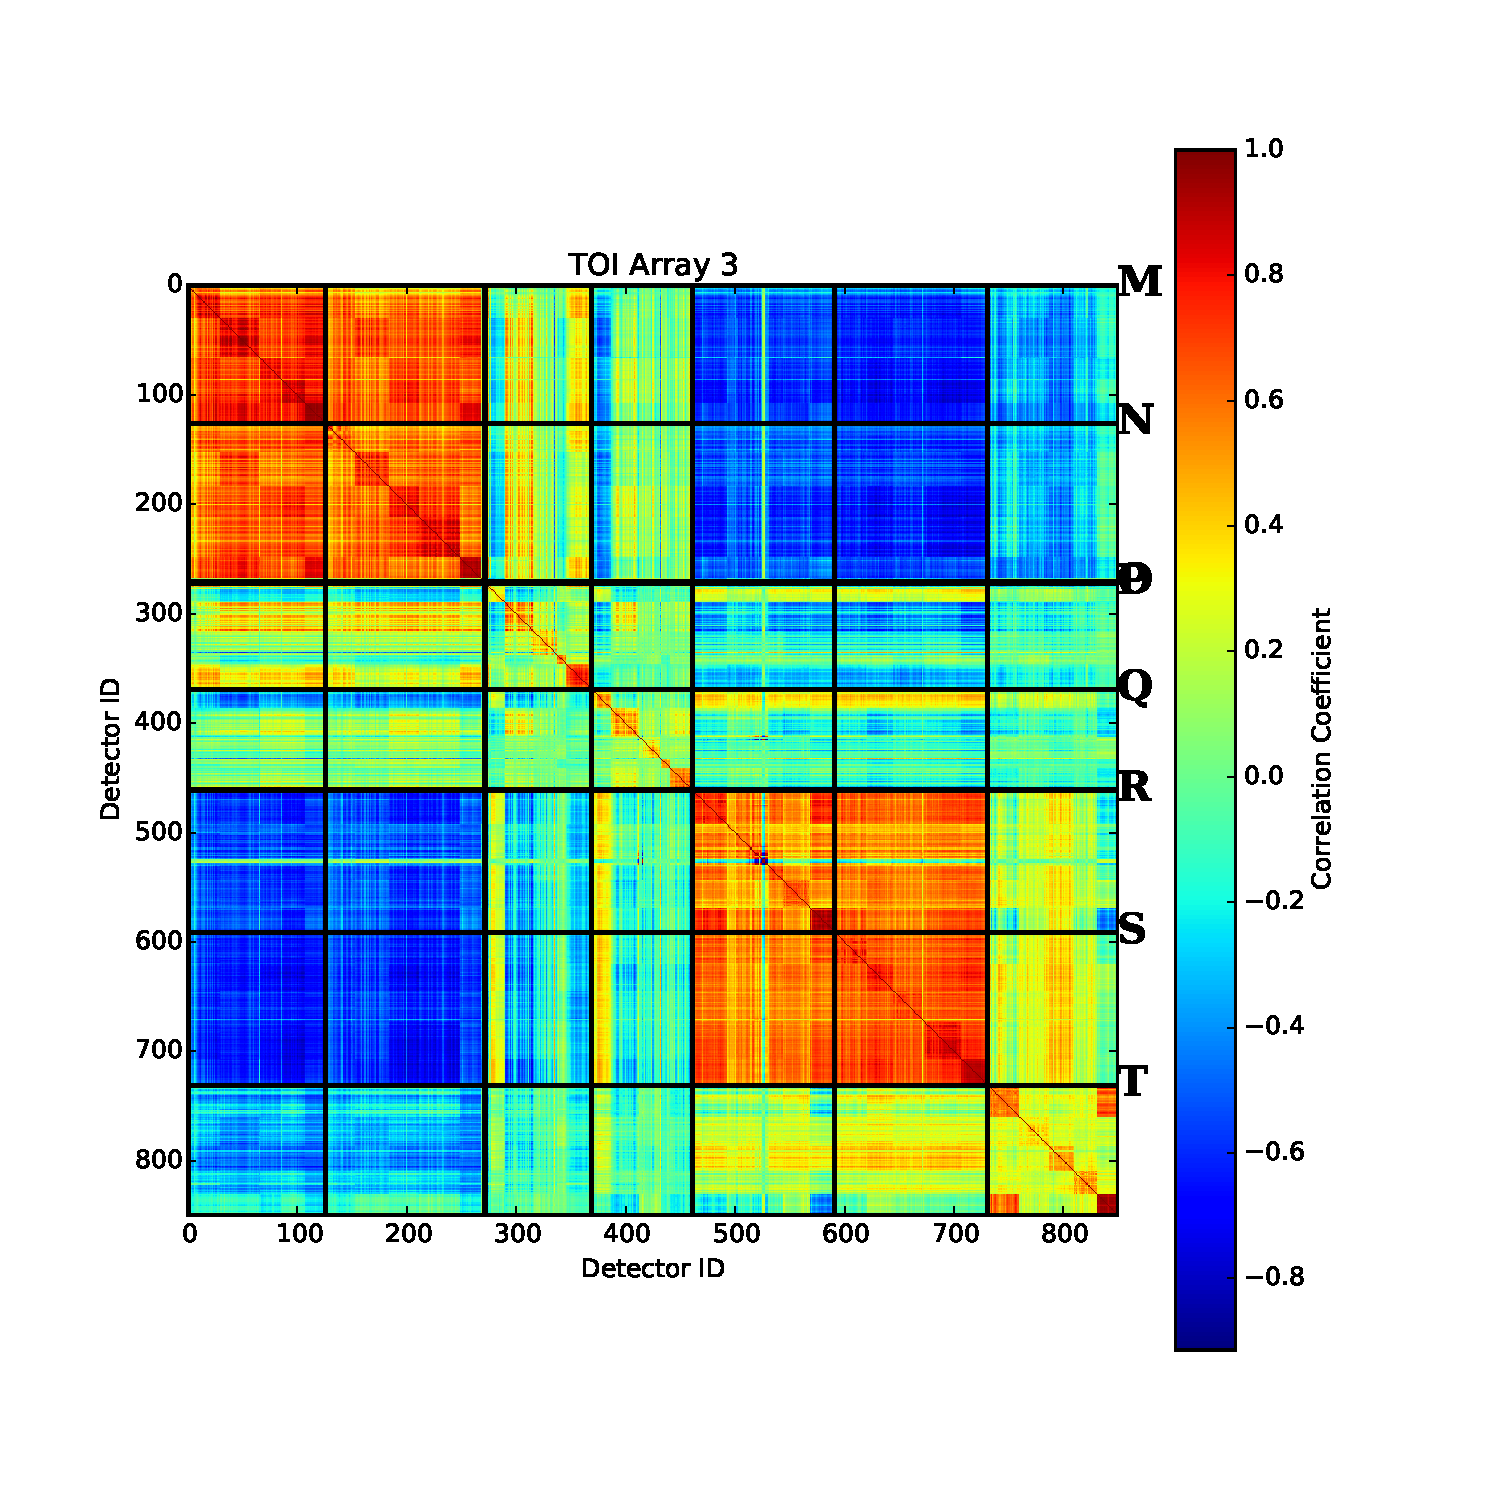
\includegraphics[width=0.3\textwidth]{Figures/NoiseTests/corrmat_TOI_CM_array_3_20170228s151.pdf}
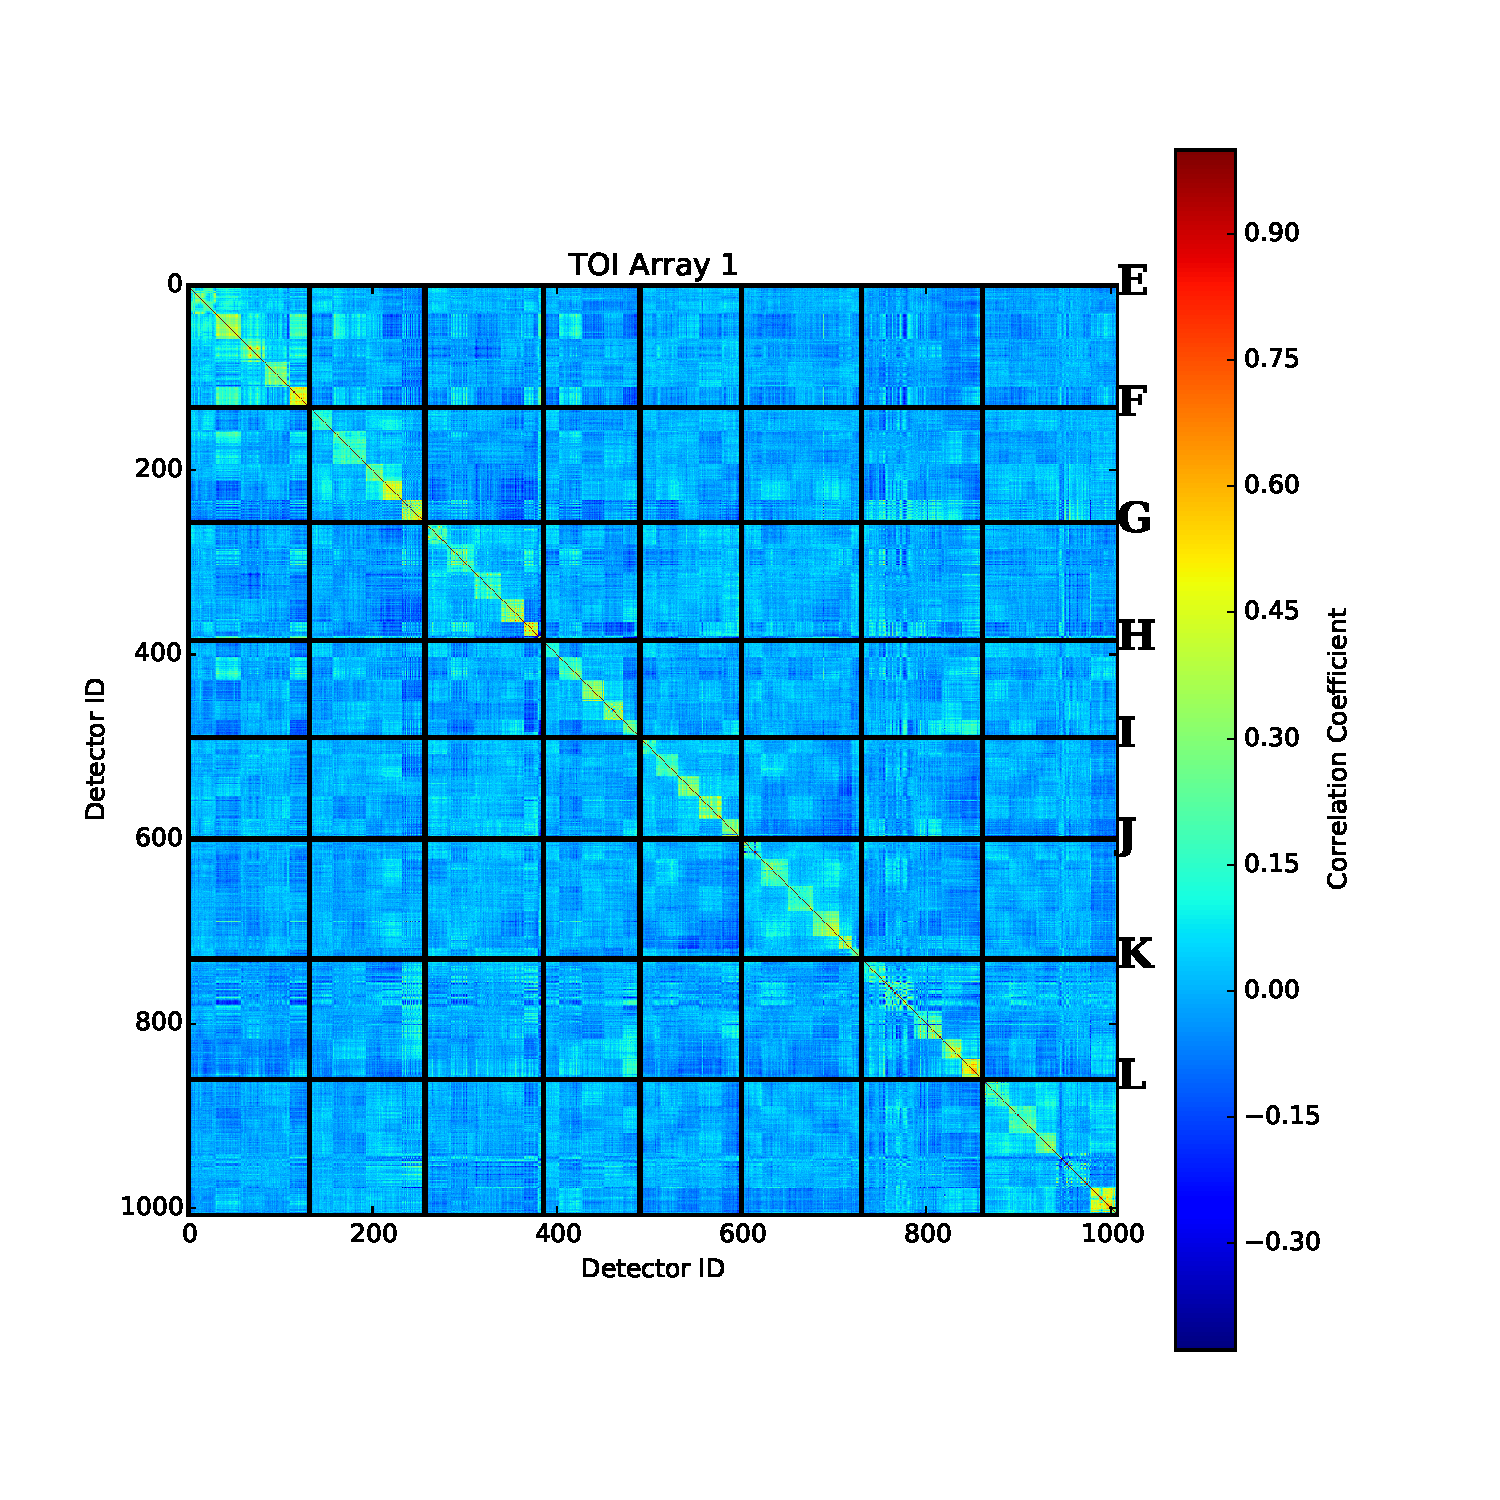
\includegraphics[width=0.3\textwidth]{Figures/NoiseTests/corrmat_TOI_PCA_array_1_20170228s151.pdf}
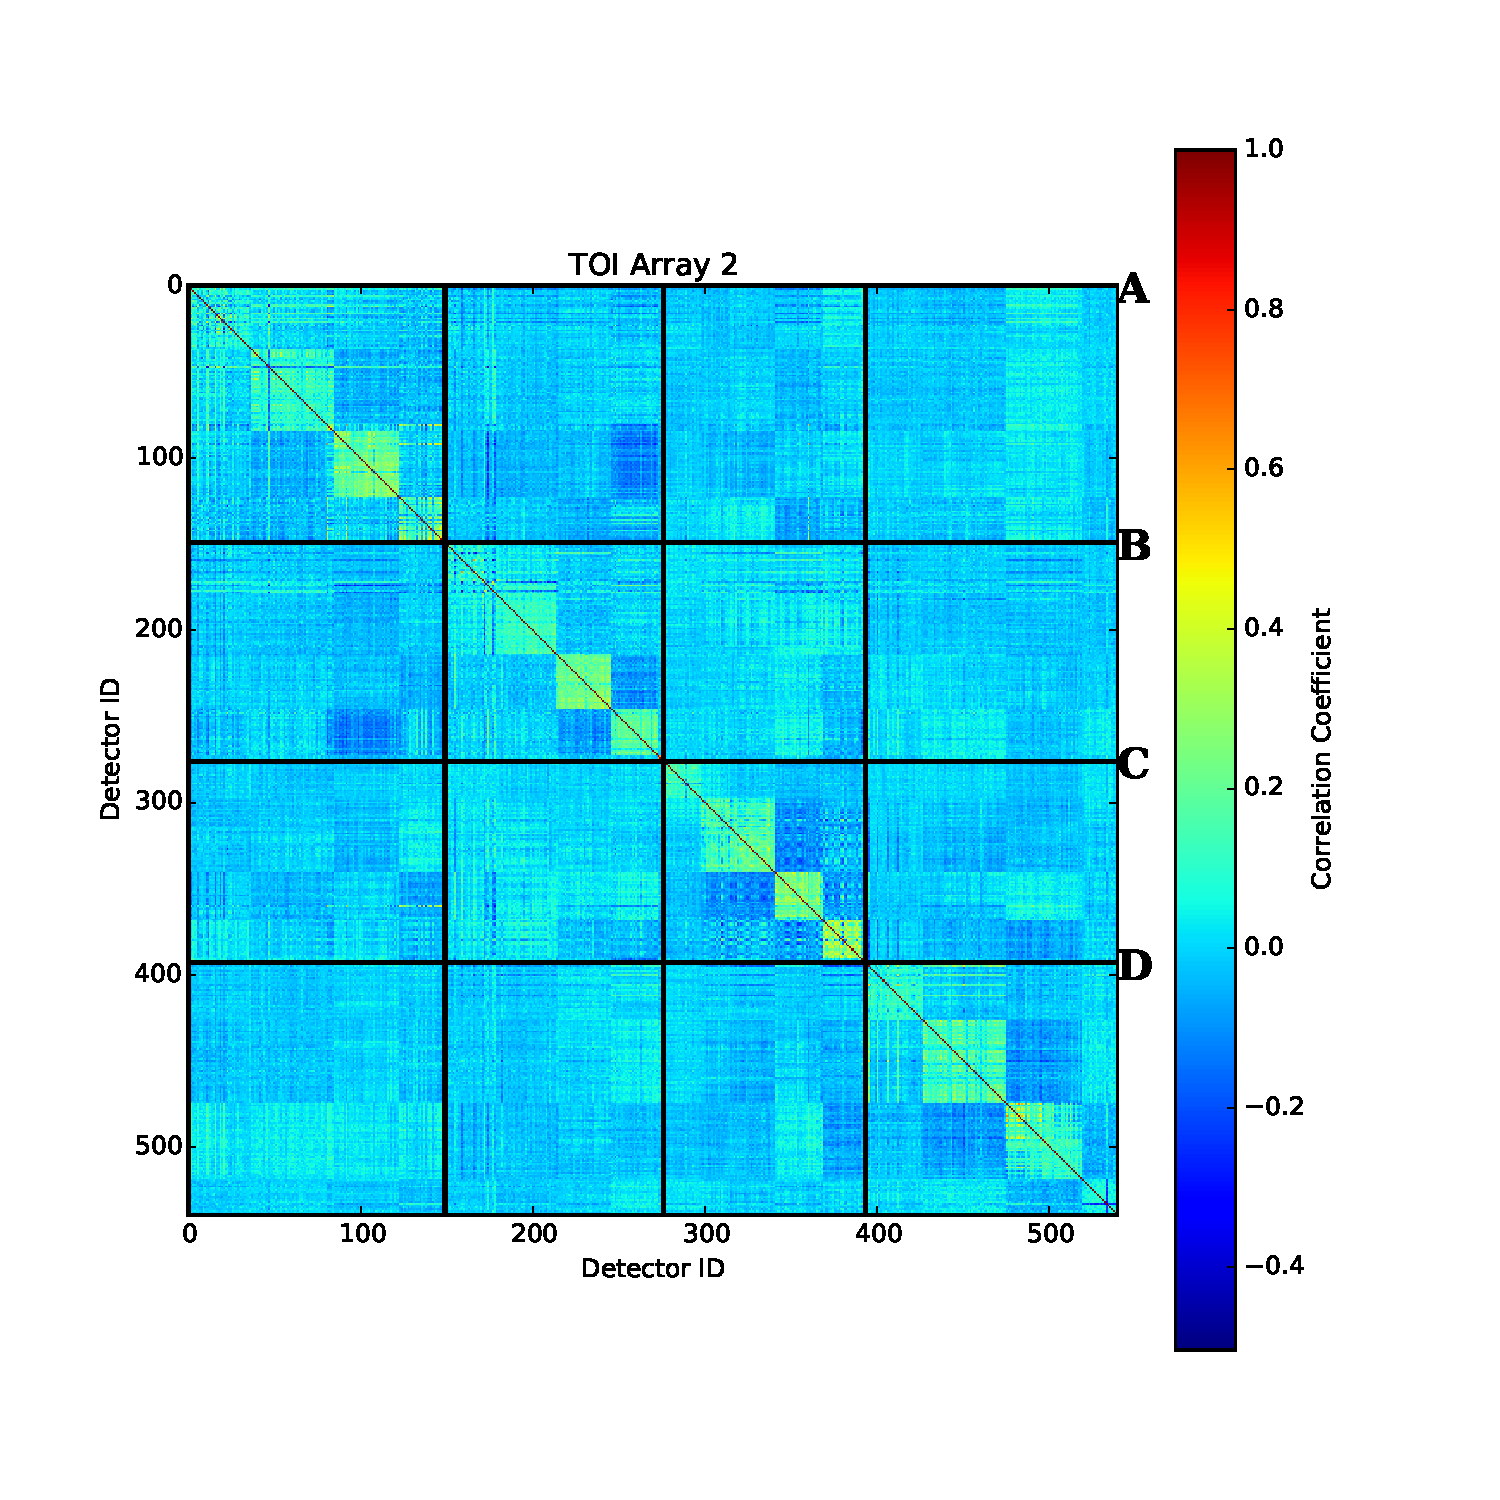
\includegraphics[width=0.3\textwidth]{Figures/NoiseTests/corrmat_TOI_PCA_array_2_20170228s151.pdf}
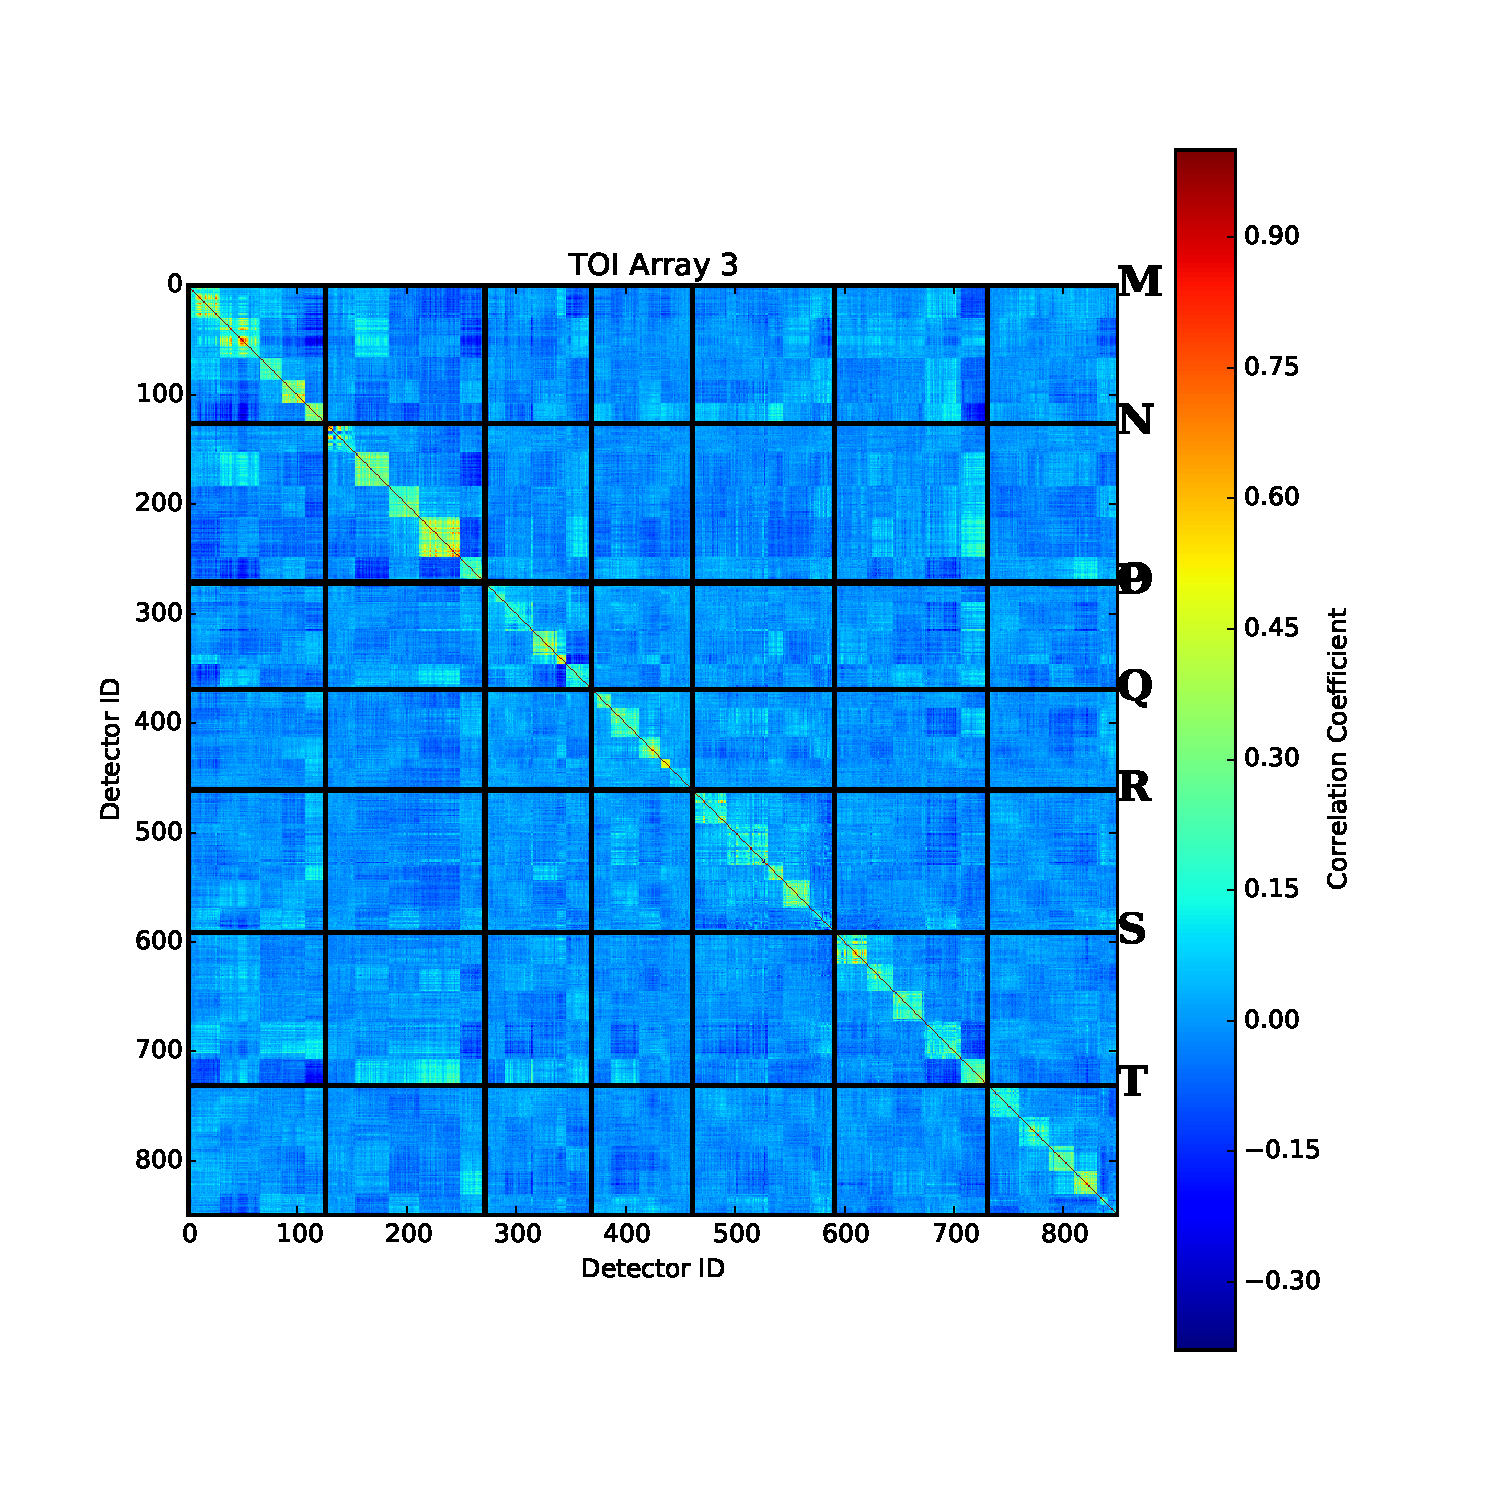
\includegraphics[width=0.3\textwidth]{Figures/NoiseTests/corrmat_TOI_PCA_array_3_20170228s151.pdf}
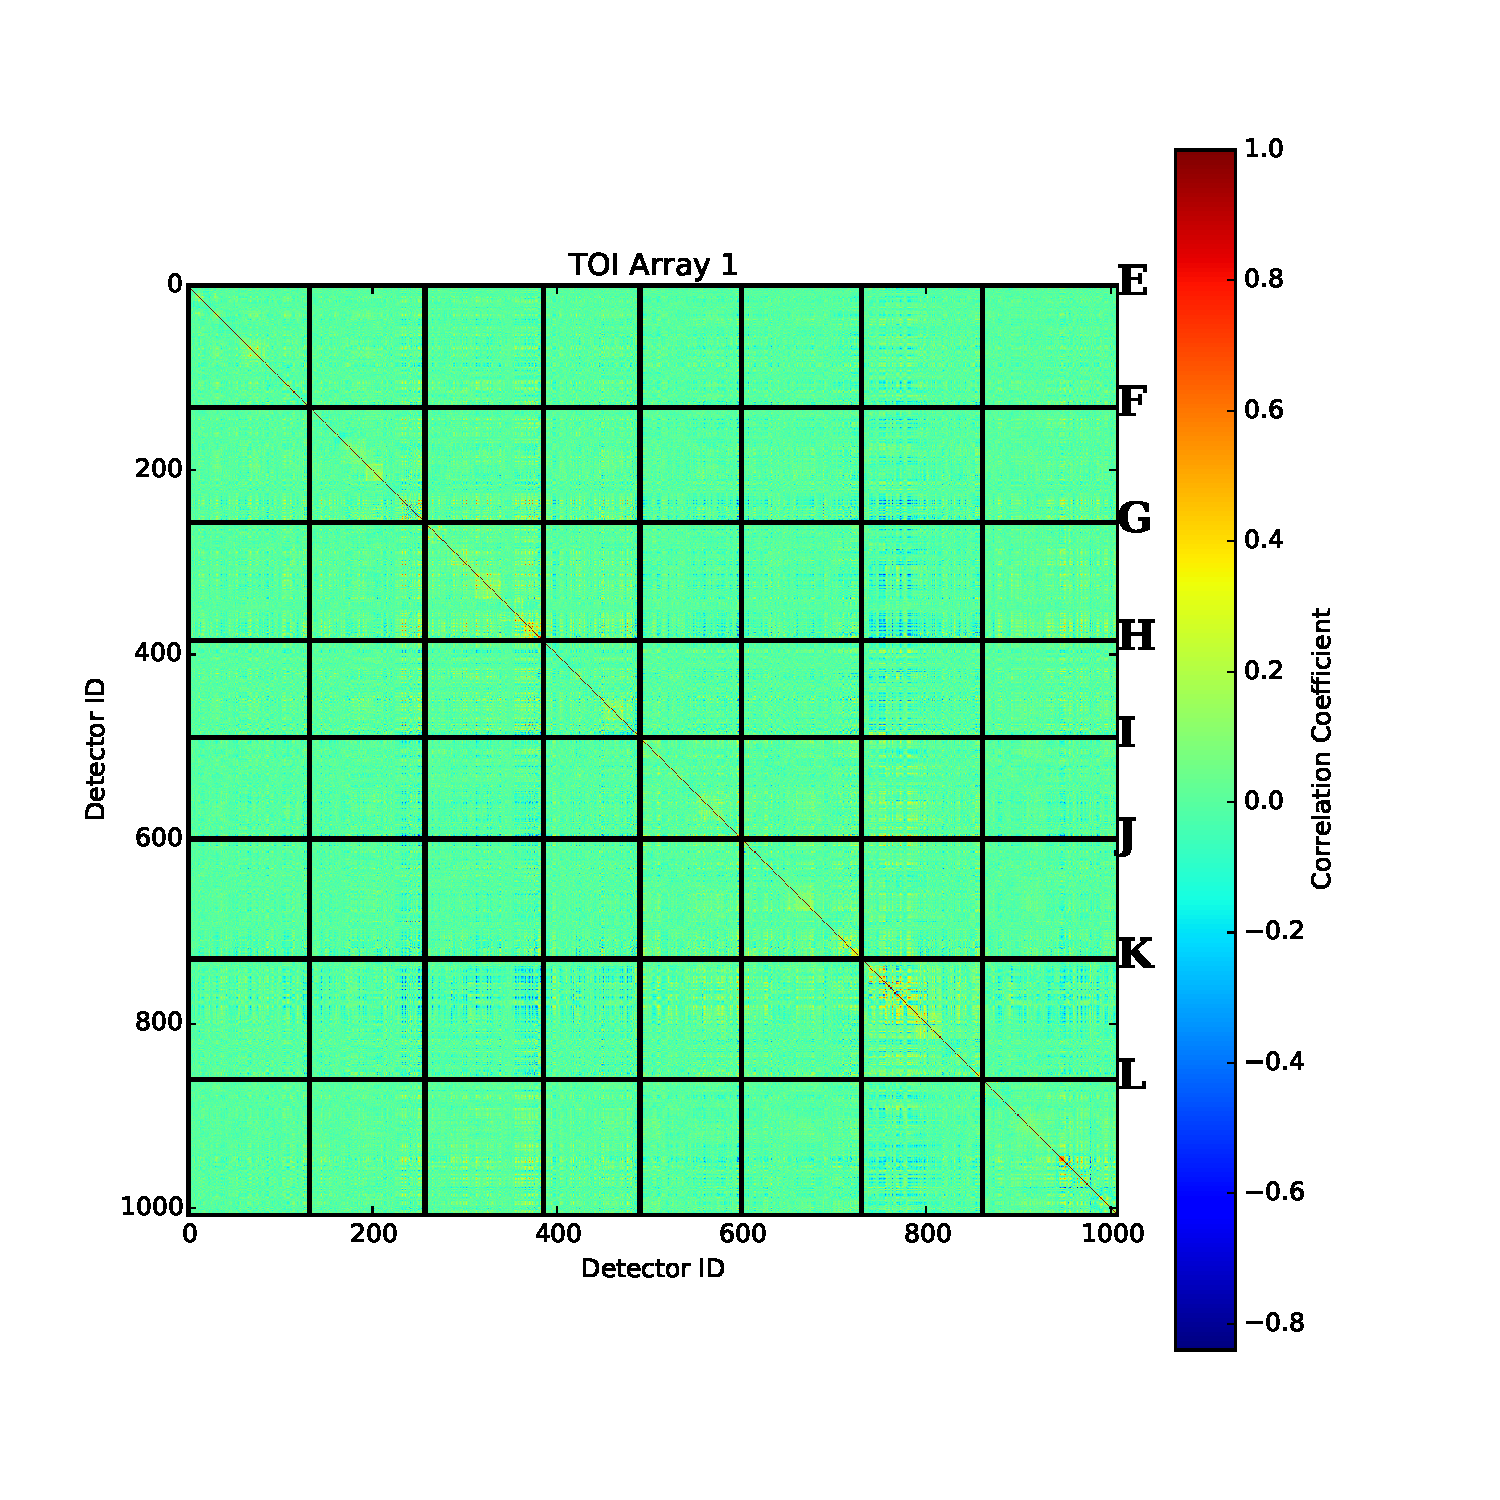
\includegraphics[width=0.3\textwidth]{Figures/NoiseTests/corrmat_TOI_BCP_array_1_20170228s151.pdf}
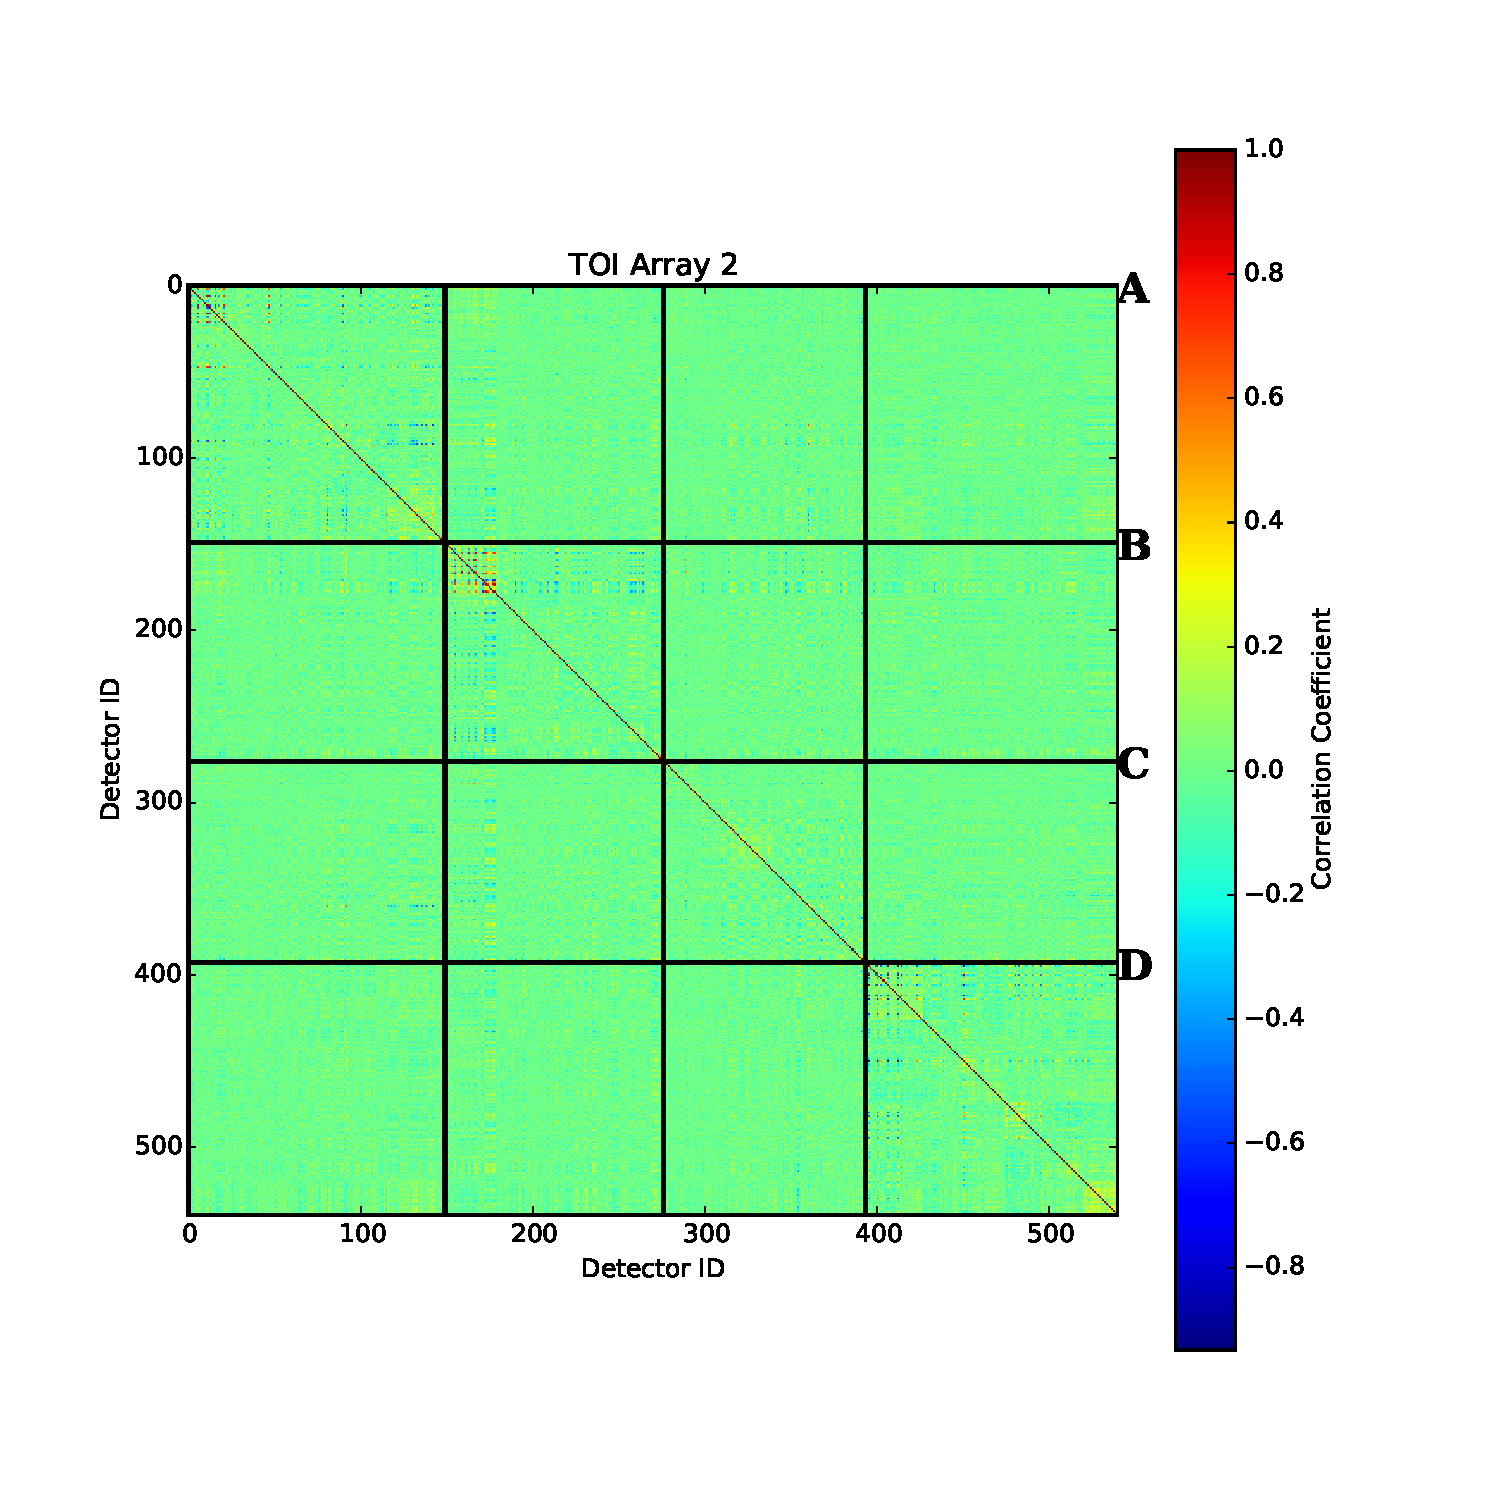
\includegraphics[width=0.3\textwidth]{Figures/NoiseTests/corrmat_TOI_BCP_array_2_20170228s151.pdf}
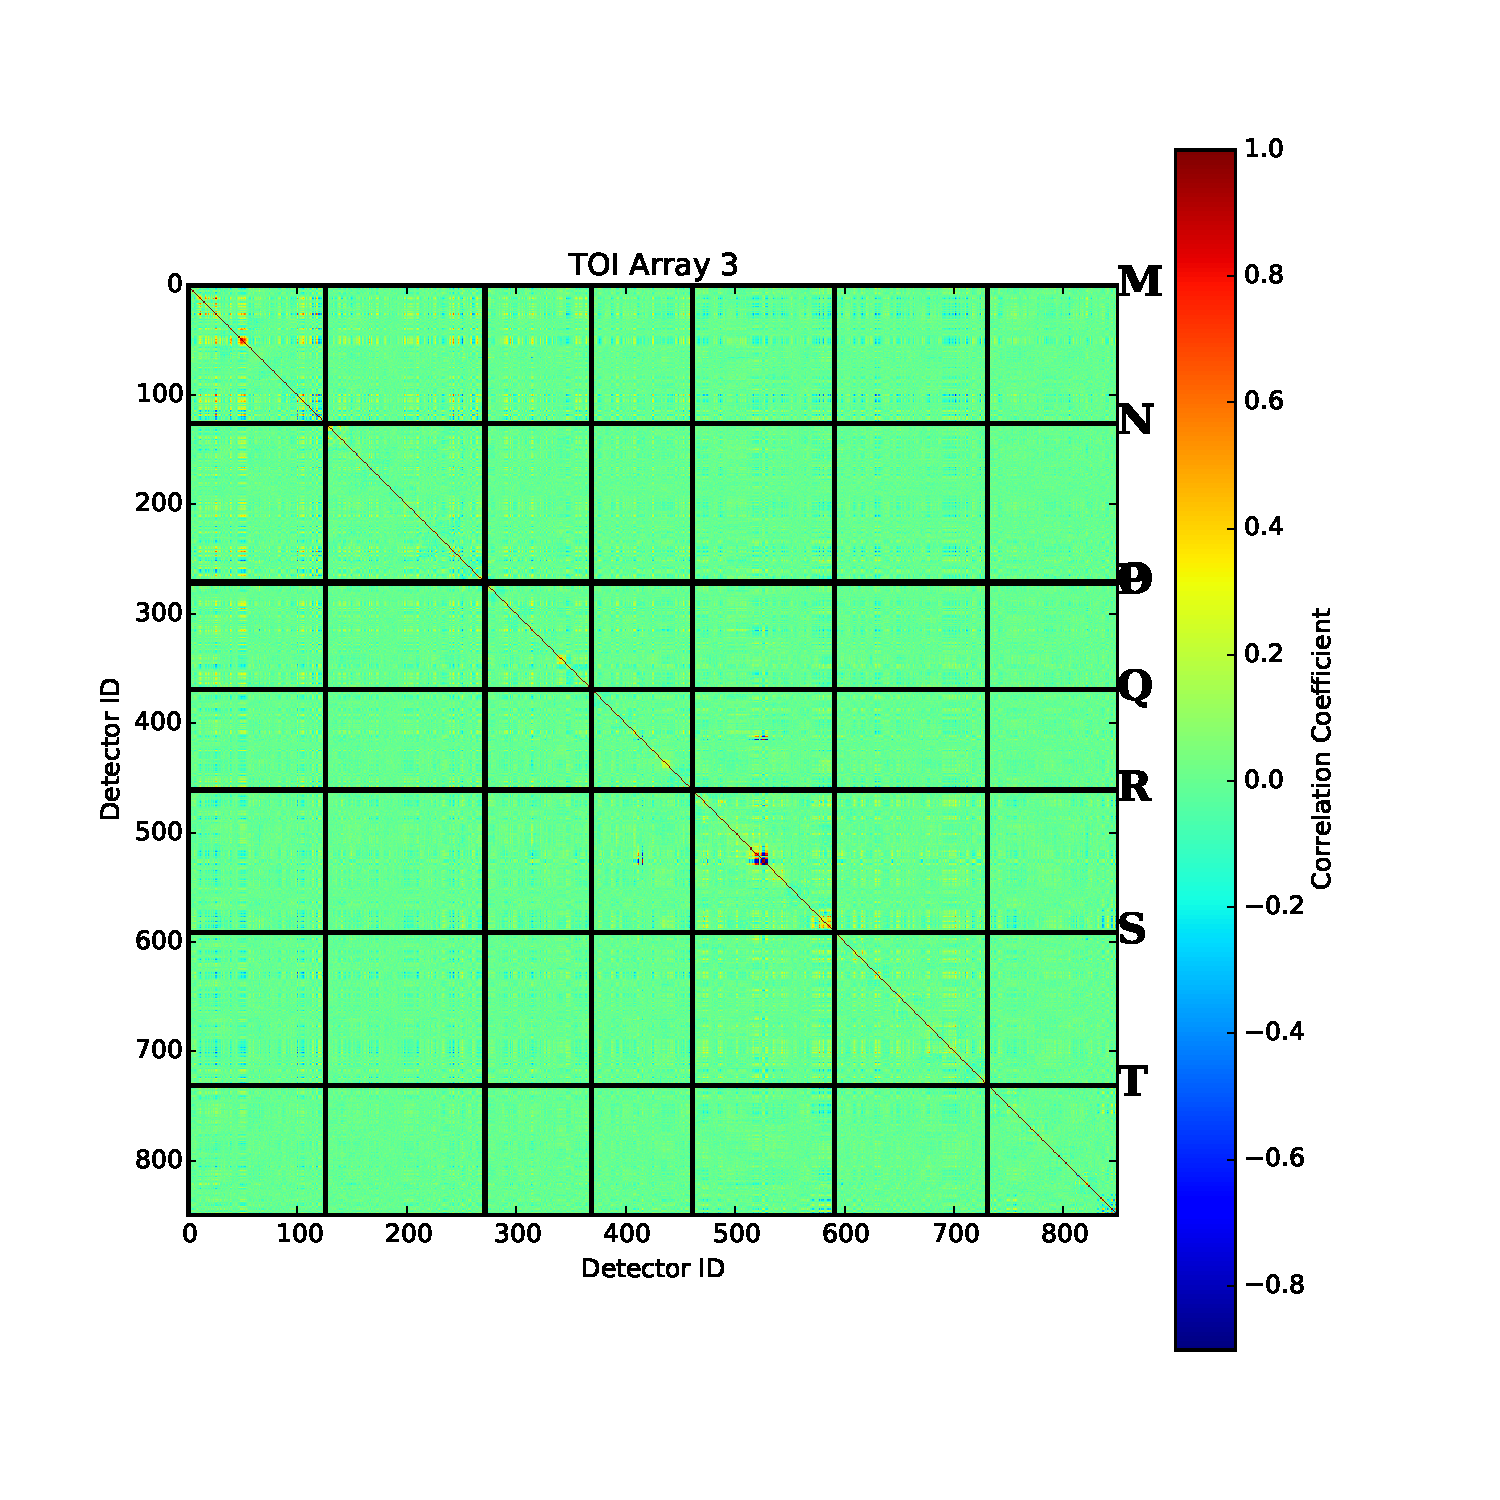
\includegraphics[width=0.3\textwidth]{Figures/NoiseTests/corrmat_TOI_BCP_array_3_20170228s151.pdf}
\end{center}
\caption[KID-to-KID correlation matrices]{\emph{From left to right:} TOI correlation
  matrices for the three NIKA2 arrays (A1, A2, and A3) for scan
  20170228s150. From top to bottom we present the correlation of the raw data,
  after CM, PCA and MCP decorrelation methods. \label{corrmatrix}}
\end{figure}

As presented on Fig.~\ref{fig:nika_toi}, the atmosphere and the electronic noise
combine into a large low frequency component that we want to eliminate as much
as possible. Most of the atmospheric component is common to all KIDs, which is
expected because the telescope is a $30\,\rm{m}$ dish and therefore
has \new{a near field limit at 900\,km.} 

On Fig.~\ref{fig:nika_toi}, the planet Uranus is visible in the TOIs and serves as
guide to both the noise relative amplitude and the discussion about TOI
processing in the following. On Fig.~\ref{corrmatrix}, we take a scan on Pluto
where the signal is negligible compared to noise on the timescale of a scan to
focus on the noise properties. We present the KID to KID timeline correlation
matrices for the three arrays, either before any data reduction or with
different estimates of the low frequency component:

\begin{itemize}
\item {\bf Common Mode decorrelation (CM)}. We use all detectors of the same
  array to build an average low frequency component nicknamed \emph{common
    mode}. This mode is then linearly regressed and subtracted from each KID
  timeline. In this method, the \emph{common mode} at time $t$ is the median of
  all KIDs at this time $t$.

\item {\bf Principal Component Analysis (PCA)}. For each NIKA2 array
  independently we decompose the covariance matrix in principal components. From
  those we derive up to 10 independent templates corresponding to the largest
  eigenvalues that we subtract from the TOIs.

\item {\bf Most correlated pixels (\cmoneb)}. For each detector in a given array we
  identify the detectors that are most correlated to it (a minimum of
  15). Using those detectors we compute a common mode like in method CM but with
  more refinements to be valid even on bright sources (see below).
\end{itemize}

As expected the raw data
noise correlation is dominated by atmospheric noise and we observe full
correlation between detectors but for badly behaving detectors which are removed
from the analysis. Significant residual correlation and anti-correlation is
observed after CM decorrelation. This is both due to spatial changes in the
atmospheric emission (overall residuals) and to instrumental and electronic
noise characteristics (correlation blocks that can be associated to electronic
boxes).  The PCA decorrelation leads to approximately block-diagonal correlation
matrices. These observed blocks in the correlation matrix can be associated to
first order to the different sub-bands in each of the electronic boxes. In the
case of the MCP decorrelation, for which only those pixels highly correlated to
the pixel of interest are used, we observe that the correlation matrix is more
diagonal than in the two other derivations of the common mode.

\begin{figure}[ht!] % Inline image example
  \begin{center}
    % A1
    \begin{overpic}[clip=true, trim={0.5cm, 0, 0, 0.6cm},width=0.59\textwidth]{Figures/NoiseTests/rms_TOI_array_1_20170228s151_mod.pdf}
      \put(3,5){\rotatebox{90}{\scriptsize Noise RMS [arbitrary units]}}
  \end{overpic}
    \begin{overpic}[clip=true, trim={0.5cm, 0, 0, 0.5cm},width=0.40\textwidth]{Figures/NoiseTests/pws_TOI_array_1_20170228s151_mod.pdf}
      \put(2,15){\rotatebox{90}{\scriptsize P$_{\nu}$ [arbitrary units]}}
  \end{overpic}
% A3
    \begin{overpic}[clip=true, trim={0.5cm, 0, 0, 0.5cm},width=0.59\textwidth]{Figures/NoiseTests/rms_TOI_array_3_20170228s151_mod.pdf}
      \put(3,5){\rotatebox{90}{\scriptsize Noise RMS [arbitrary units]}}
    \end{overpic}
    \begin{overpic}[clip=true, trim={0.5cm, 0, 0, 0.5cm},width=0.40\textwidth]{Figures/NoiseTests/pws_TOI_array_3_20170228s151_mod.pdf}
      \put(2,15){\rotatebox{90}{\scriptsize P$_{\nu}$ [arbitrary units]}}
    \end{overpic}
    % A2
    \begin{overpic}[clip=true, trim={0.5cm, 0, 0, 0.6cm},width=0.59\textwidth]{Figures/NoiseTests/rms_TOI_array_2_20170228s151_mod.pdf}
      \put(3,5){\rotatebox{90}{\scriptsize Noise RMS [arbitrary units]}}
    \end{overpic}
    \begin{overpic}[clip=true, trim={0.5cm, 0, 0, 0.5cm},width=0.40\textwidth]{Figures/NoiseTests/pws_TOI_array_2_20170228s151_mod.pdf}
      \put(2,15){\rotatebox{90}{\scriptsize P$_{\nu}$ [arbitrary units]}}
    \end{overpic}
  \end{center}
\caption[Noise RMS and power spectra]{
  The data noise rms (left column) and power spectra (right column) are shown for the three NIKA2 arrays (A1, A3, and
  A2 from top to bottom) for scan 20170228s151. The rms and power spectra are given for the raw
  data (blue), and for the CM (green), PCA (red) and MCP (cyan) decorrelated
  data. The vertical lines in the rms noise figures separate detectors from
  different readout electronic boxes. Within each electronic box the pixels are
  ordered with increasing resonant frequency across the electronic
  band. 
  \label{rmspws}}
\end{figure}

In Fig.~\ref{rmspws} we present the rms noise per KID and the power spectra of
a typical raw datastream, and the CM, PCA and MCP decorrelated data. We observe that after
decorrelation we reduce significantly the rms of the
noise. Equivalently, the $1/f$-like noise in the power spectra
(principally due to atmospheric emission)
is significantly reduced leading to nearly flat spectra down to 0.05 Hz, with
larger $1/f$-like residual noise for the CM decorrelation method at lower
frequencies. This is translated into a larger rms noise for this method with
respect to the others. For the three arrays we find increasing noise with
increasing resonant frequency within each electronic box. This is probably
related to the difference of gains between subbands in the readout
electronics. We also find for the three arrays some noise bursts that are not
fully consistent from one decorrelation method to another. \\

We have investigated several ways of using this information to remove this
component from the TOIs. Our prefered choice so far, that is the reference
method for this document, is the \cmoneb\ method, that we describe into further
details below:

\begin{itemize}
\item From the pointing information (Sect.~\ref{se:ptg}), we derive a mask per TOI
  and for each time $t$ that is 0 if the KID is close to the source, 1
  otherwise. \vu{In the case of a point source, the mask consists in 
    a radius of 60\,arcsec centered on the source, whereas for
    diffuse emission, tailored masks are build.}
\item Only samples for which two KIDs are far from the source,
  \vu{hence which are not discarded using the mask,} are selected and the KID-to-KID
  correlation is computed.
\item For a KID $k_0$, we store the KID identifiers that are most
  correlated to it. We first select the 15 most correlated KIDs, then 
  the average and the dispersion $\sigma$ of these correlations are
  computed. \vu{Then we add to the selection all the KIDs that are as correlated to $k_0$ as the
  15 first, up to $2\,\sigma$.}
\item A median common mode (far from the source) for this block of 15
  or more KIDs is derived.
\item A cross-calibration to each of these KIDs is computed using the
  median common mode. Then an inverse noise weighted average mode is build. At each time, we use
  only KIDs \vu{that are not discarded with the source mask.}
  At this stage it is important to verify to have enough KIDs to produce a
  continuous mode and to do not leave samples without any estimation.
\item We linearly regress this average mode against $k_0$'s TOI (far from the
  source) and subtract on the entire $k_0$ timeline.
\end{itemize}

This process is repeated for each KID. Fig.~\ref{fig:nika_toi} shows an example
of this low frequency mode derivation, together with the resulting TOI
cross-correlation matrix after its subtraction. We have tested on simulations
that this method does not alter the flux of the
source.

If the observed field contains something else than a single point source at its
center, then several options are available to generalize this method. In
particular, the mask can be designed to adjust to several point sources. If the
source is diffuse and extended, then we may go through an iterative procedure that
subtracts an improved derivation of the signal at each step. For this work about
the commissioning of the instrument and the assessment of its performances on
point sources, we do not need to go into further details about this.

\subsection{Map projection}
\label{se:map_projection}

At this stage, data have been calibrated and cleaned and we have the pointing
information for each sample. If the noise was white and uncorrelated from KID to
KID, we would be able to produce an optimal map $S_p$ using an inverse
variance noise weighting of all of the measurements $m^k_t$ that fall
into a map pixel $p$ with a simple Nearest Grid Point procedure. In
this scheme, data samples are coadded with inverse variance noise
weighting: for each KID, we compute the standard deviation
$\sigma_k$ of its TOI far from the source (see Sect.~\ref{se:toi_proc}). Each
sample of this KID therefore has a weight of $1/\sigma_k^2$ and

\begin{eqnarray}
S_p        &=& \frac{1}{\sum_{k,t}1/\sigma_k^2}\sum_{k,t} \frac{m^k_t}{\sigma_k^2}\,, \label{eq:ngp_sum}\\
\sigma^2_p &=& \sum_{k,t}1/\sigma_k^2\,, \label{eq:ngp_var}
\end{eqnarray}

where $\sigma^2_p$ is the variance associated to pixel $p$. The
pipeline automatically projects one map per array and a combined 1\,mm
map and takes a small enough resolution to respect the Nyquist
criterion on the beam sampling.
To keep margin
and for the sake of simplicity, we usually take 2\,arcsec resolution pixels.

In practice, and although the data cleaning procedure described in
Sect.~\ref{se:toi_proc} significantly reduces the low frequency component of
TOIs, the residual noise is still not completely white nor KID independent. The
correlation matrix is not strictly zero to begin with (Fig.~\ref{fig:nika_toi})
and when looking at the distribution of the SNR on maps and variance maps
obtained with Eqs~(\ref{eq:ngp_sum},\ref{eq:ngp_var}), the distribution is
Gaussian, but not normalized to unity (see Fig.~\ref{fig:sigma_boost}). This is
due to the remaining correlations between TOIs before projection. At this stage,
rather than putting more effort in TOI processing, we renormalize the width of
the Gaussian noise, which actually increases the map variance by the required factor
so that the SNR distribution becomes normalized. This normalization factor
varies from scan to scan but it is usually between 1.2 and 1.5. It is estimated on
the background of the map, i.~e. far from the source.

\begin{figure}[ht!]
\begin{center}
\includegraphics[clip, angle=0, scale=1, width=0.75\textwidth]{Figures/sigma_boost.eps}
\caption[Distribution of the SNR per beam]{Histogram of the SNR per beam on a scan of weak source (G2, see
  Sect.~\ref{se:nefd_estimation_methods}). While the histogram is Gaussian, its
  width is not normalized to 1 due to residual correlated noise between the
  TOIs. This factor is accounted for before delivering the final variance map
  and associated flux estimates.}
\label{fig:sigma_boost}
\end{center}
\end{figure}

When several scans of the same source are averaged, we apply an inverse
variance weighting as well. Weights are taken from the variance maps of each scan,
corrected for the excess variance mentioned in the previous paragraph. The
final variance map of the sum of scans is also corrected for such a factor if necessary.

\subsection{Photometry}
\label{se:intro_photometry}

Throughout this document, we adopt the following convention. Assuming the beam
is a perfect Gaussian of known $FWHM=\sigma\sqrt{8\ln 2}$, the instantaneous
signal measured by a KID is

\begin{equation}
m^k(x,y) = \phi e^{-(x^2+y^2)/2\sigma^2} = \phi G(x,y)
\label{eq:flux_per_beam_def}
\end{equation}

with $\phi$ the flux of the source \vu{and $(x,\, y)$ the coordinates in
the chosen system.} In practice, the beam is not a perfect Gaussian
and significant side lobes must be accounted for
(Sect.~\ref{se:beams}). If the beam was perfectly known and stable, we could in
principle replace the Gaussian form in Eq.~\ref{eq:flux_per_beam_def} by the
beam pattern and fit for the amplitude $\phi$.
%In practice, we have found that
%it was enough as a first approximation to take an equivalent effective Gaussian
%width and use it to derive the beam template.
\sam{In practice, the beam pattern i) has a complexe structure, including
features which can rotate with the observation elevation (as presented
in Sect.~\ref{se:fullbeam}), ii) has a few percent dispersion across the FOV (see
Sect.~\ref{se:MB}) and iii) shows some variations with the observation date
(see Sect.~\ref{se:obsdate_variations}). However, we have found that using an equivalent
effective fixed-width Gaussian for the photometry, as presented in
Sect.~\ref{se:cal_HA_main}, is sufficient to ensure accurate, stable and robust flux
measurements, as assessed in Chapt.~\ref{se:photometry}. The reference fixed-width
Gaussian is chosen sizably larger than the measured main beam width
(see Sect.~\ref{se:MB}) to account for a fraction of the
signal stemming from the error beams and side lobes.} Namely, we take
12.5 and 18.5\,arcsec FWHM at 1 and 2\,mm respectively and compute all our fluxes with these
values. We do this for both absolute calibrators (see Chapt.~\ref{se:calibration})
and analyzed point sources (see Chapt.~\ref{se:photometry}) to be consistent. Our
photometric system is further detailed in
Sects.~(\ref{se:cal_HA_reference}, \ref{se:cal_HA_main}).


Let's call $s_p$ the measured signal at map pixel $p$ and denote by $g_p$ the
Gaussian weight given to pixel $p$ as a function of its distance to the source,
as defined in Eq.~\ref{eq:flux_per_beam_def}. The amplitude fit is performed
with an usual maximum likelihood approach. We assume that the renormalization of
the variance map described in the previous section is enough to account for the
residual noise correlations from pixel to pixel and therefore assume the pixels to
be independent in this estimator:

\begin{eqnarray}
\hat{\phi} &=& \frac{1}{\sum_p g_p^2/\sigma_p^2}\sum_p
s_p\frac{g_p}{\sigma_p^2} \label{eq:flux_estim_def} \\
\sigma^2(\hat{\phi}) &=& \frac{1}{\sum_p
  g_p^2/\sigma_p^2} \label{eq:flux_estim_var_def}
\end{eqnarray}

In the case of Gaussian white noise, this maximum likelihood estimator coincides
with the classical minimum variance estimator and thus provides the best SNR
estimate of the source flux.

%% \subsection{Opacity correction}
%% 
%% Water vapor along the line of sight absorbs power from the source and therefore
%% biases the flux measurement. At the same time, the overall airmass acts as a
%% diffuse source of power on the KIDs that induce a variation of their resonance
%% frequency. We are able to calibrate it and therefore derive the opacity in real
%% time from \nika\ data. This is described in details in
%% Sect.~\ref{se:opacities}. Suffice is here to say that after the derivation of
%% the KID offsets and their relative gains as described in
%% Sect.~\ref{se:fov_first_geometry}, one we know the opacity, we can derive an
%% absolute calibration per KID.

%% \subsection{Absolute calibration}
%% \todo{See how to talk about Planet models and repeated observations of these to derive
%% the ``final'' abs. cal for the run.}
%% 
%% %The data reduction of \nika\ cannot be done exclusively KID by KID
%% %independently. Each matrix is a filled array with more than one detector per PSF
%% %and the atmosphere together with the electronics chain act as correlated
%% %noise. We therefore have to work iteratively to improve both individual and
%% %global parameters of the detectors. In this section, we give an overview of the
%% %full data reduction that illustrates this iterative process. More details on
%% %each specific step are given in other dedicated sections.
%% 
%% \subsection{Overview of the on-sky calibration method}
%% 
%% The steps to go from raw timeline data in Hertz to calibrated data in Jansky per beam comprize:
%% \begin{itemize}
%% \item[] Opacity correction
%% \item[] Field-of-view geometry and KIDs selection
%% \item[] KID-to-KID intercalibration (flat fielding)
%% \item[] Absolute calibration  
%% \end{itemize}
%% 
%% 
%% \subsection{Data reduction summary {\color{blue} Nico}}
%% 
%% The performance assessment relies on a data reduction pipeline that consists of the following steps:
%% \begin{itemize}
%% \item[] reading of the raw timeline 
%% \item[] implementation of the calibration
%% \item[] substraction of the correlated part of the noise 
%% \item[] projection of the timeline onto maps
%% \end{itemize}


%%	OBSERVATION MODES
%% This section presents the different kind of observations that we have
%% performed to derive the pipeline parameters and performances that are
%% presented in details in the followin sections.
%\label{se:observation}

\section{Calibration and commissioning observations at the 30\,m telescope}% {\color{YellowGreen} Nico}}

This section presents the different observation modes that have been used with
\nika\ for both commissioning and scientific purposes. Some of them are common
to usual IRAM observing modes (e.g.~''on the fly'' raster scans), some of them
have been designed specifically for \nika\ (e.g.~the focus sequence). We start
by a short overview of a typical set up sequence at the beginning of
an observational run. This
will put each observation mode in perspective. Then we go into more details
about the performances of the system.

\subsection{Overview of different types of scans}

Once the KIDs are tuned and \nika\ is ready for observations, before actually
observing a scientific target, one needs to adjust the focus and pointing of the
telescope. In the case of EMIR typically, these two parameters are adjusted iteratively by
alterning ``pointing'' (\aka\ ``cross'') and ``focus'' scans to optimize the
centering of a bright point source on a reference detector and to maximize the
incoming flux on it. With \nika\ , mostly due to absence of horns, this
procedure is not optimal. Indeed, it was noticed that the position of the source
moved by several arcsec with the displacement of M2
\vu{during the focus procedure} and this would alter the flux
measurement on a fixed reference position too much to enable focus
optimization.

To solve this issue we have designed a specific focus procedure that takes
advantage of the dense sampling of the FOV that allows to map a source with only
a few subscans. We perform a series of five successive short raster scans of a
bright point source at five M2 position offsets along the optical axis.%, typically
%$\{-0.8, -0.4, 0, 0.4, 0.8\}$\,mm w.r.t.~the current $z$-focus (which
%is usually the previous optimal $z$-focus value).
We then analyse each map to optimize the $z$ position of M2. More details are given in
Sect.~\ref{se:axial_focus}.
Once the focus is correctly determined, the pointing
corrections are derived from an EMIR like pointing calibration scan
(Sect.~\ref{se:pointing}). The instrument is then ready to observe scientific
targets.

\subsection{Axial focus}
\label{se:axial_focus}

\begin{figure}[ht!]
\begin{center}
  %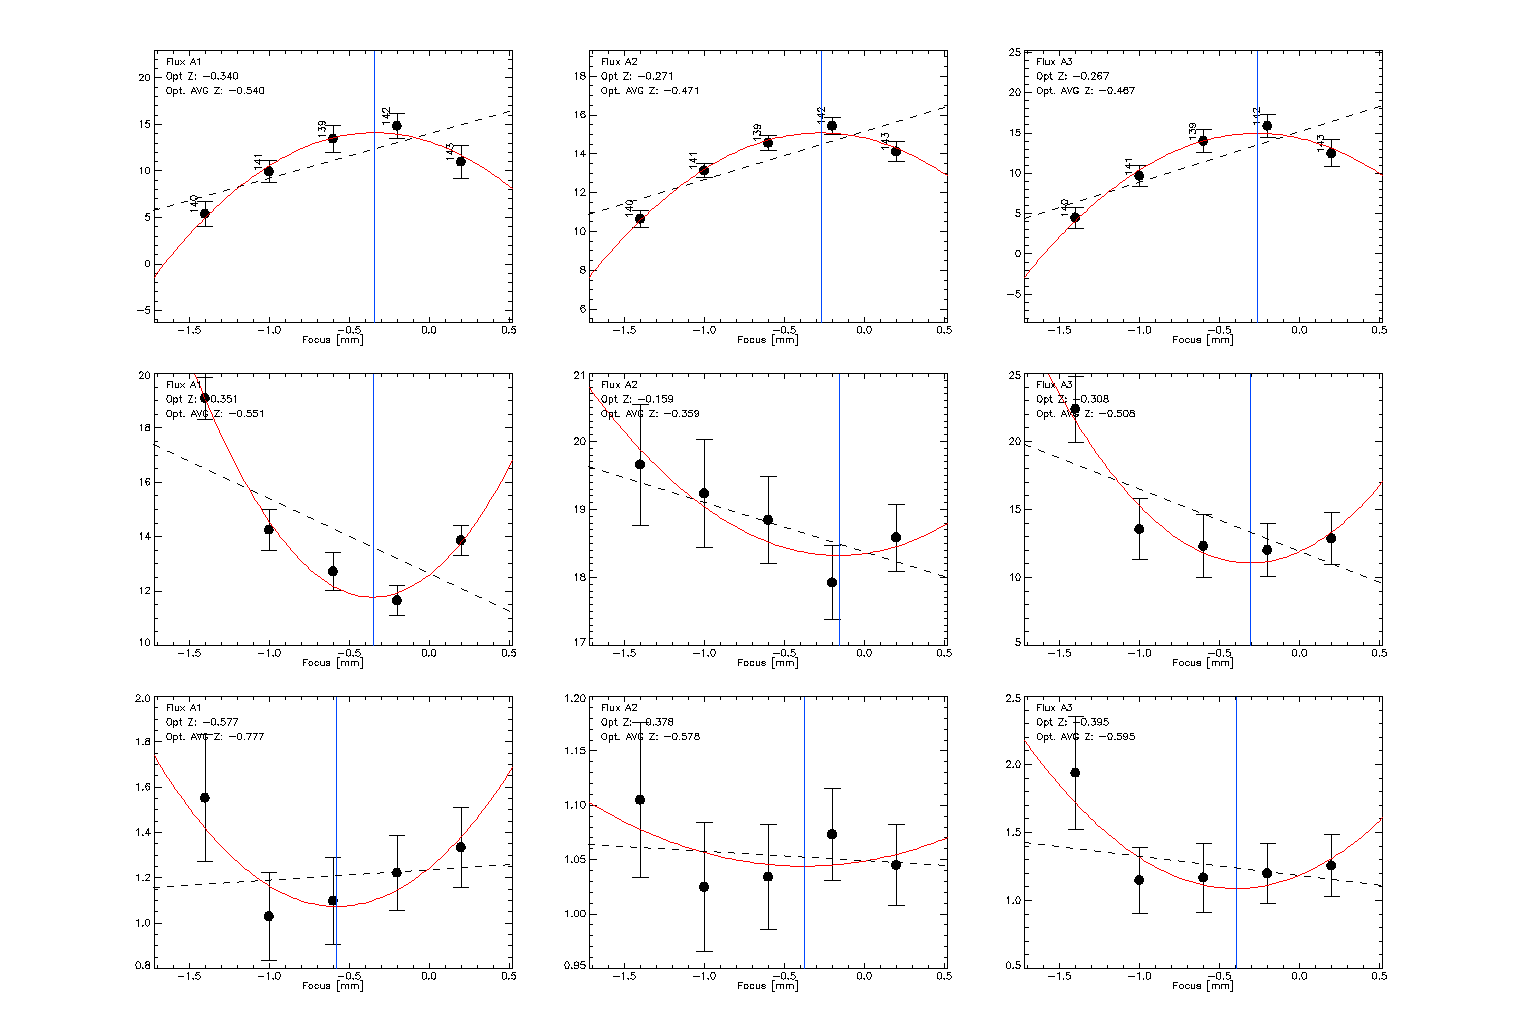
\includegraphics[clip, angle=0, trim={1.5cm, 1cm, 1.5cm, 1cm},
  %width=\textwidth]{Figures/plot_20170419s143.png}
  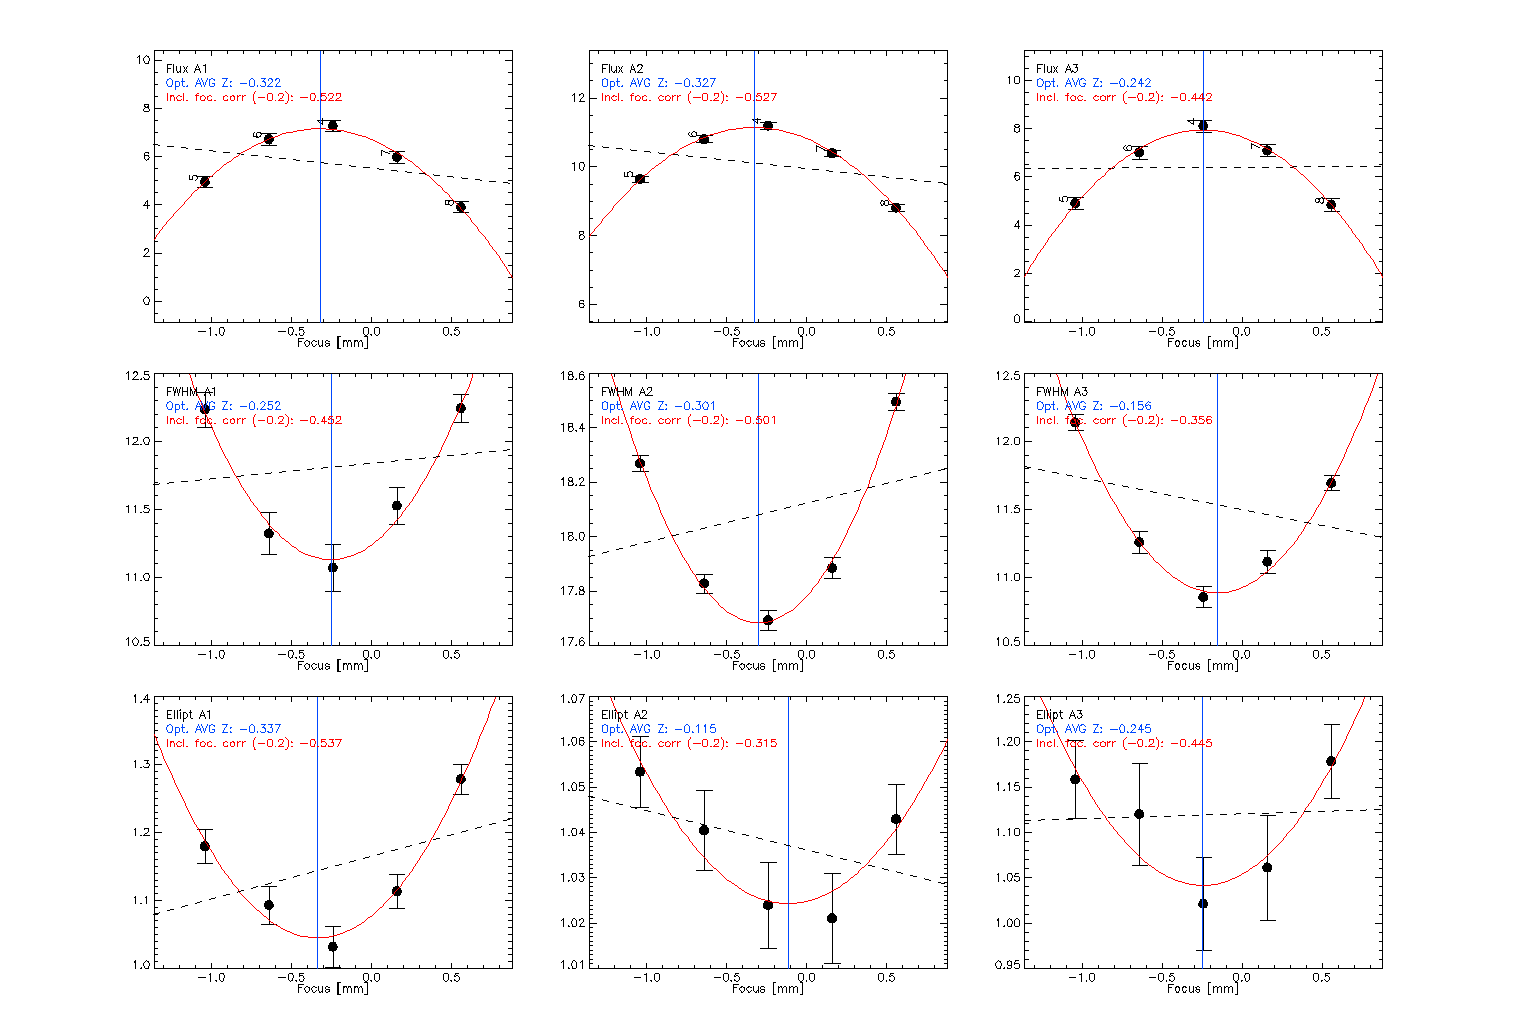
\includegraphics[clip, angle=0, trim={3cm, 0.5cm, 3cm, 1.5cm}, width=\textwidth]{Figures/plot_20180120s8_zfocus.png}
\caption[Axial focus measurement]{Example of axial focus measurement using a
  \emph{focus$\_$OTF} observation of the bright quasar 3C84 (\aka\ 0316+413) during N2R14 in good observing conditions (scans ID: from '20180120s4' to '20180120s8'). \vu{Flux (first
  row), FWHM (second row) and ellipticity (third row) measurements are
  shown as a function of the axial focus offsets for Array 1 (first
  column), Array 2 (second column) and Array 3 (third column). The
  best-fitting parabola is shown in red. To help the observer
  assessing the parabolic fit quality, the best-fit linear model is also drawn
  with dashed black lines.} 
  The blue vertical line locates the best-fitting $z$-focus value of
  each fit. The optimal focus values derived from flux
  maximization and FWHM minimization agree to better than 0.1\,mm in these
  conditions of observation. While ellipticity may be often regarded as a confirmation
  more than a decisive criterion (due to larger uncertainty on its measure), the
  associated minimum is also in good agreement with the values derived from flux
  and FWHM measurements in this example taken in stable atmospheric conditions.}
\label{fig:focus-example}
\end{center}
\end{figure}

The best axial focus in the central region of the arrays is estimated using the
so-called \emph{focus$\_$OTF} PAKO script, which produces a series of five $1'
\times 5'$ OTF scans at various values of the focus in $0.4~\rm{mm}$ steps
around an \emph{a priori} value $z_0$, namely
$z \in \{-0.8, -0.4, 0, 0.4, 0.8\} + z_0$.
Elliptical Gaussian fits on the reconstructed maps provide estimates of
the flux and FWHM along minor - and major - axes for each focus. Parabolic fits are
then used to determine the best focus. We consider three estimates: i) $\hat
z_{\rm{peak}}$ the focus that maximizes the estimated flux, which is the
amplitude of the 2D Gaussian, ii) $\hat z_{\rm{fwhm}}$ the focus that minimizes
the geometrical FWHM, defined as the quadratic mean of $\rm{FWHM}_{\rm{major}}$
and $\rm{FWHM}_{\rm{minor}}$, and iii) $\hat z_{\rm{ellipt}}$ the focus that
minimizes the beam ellipticity, defined as
$\rm{FWHM}_{\rm{major}}/\rm{FWHM}_{\rm{minor}}$. Fig.~\ref{fig:focus-example}
shows an example of such a sequence. When deciding on the focus to apply, we
give priority to the optimal flux, taking an average between values on A1 and
A3: there is little difference between the two and the 2\,mm channel is
less sensitive to the focus change than the 1\,mm.

As presented in more details in Sect.~\ref{sec:focus_surfaces}, the focus
surface is not strictly flat across the FOV. The way sources are scanned in
this \emph{focus\_OTF} sequence is designed to save time but it gives more weight
to the central KIDs. Hence, the optimal focus derived from the fits is
biased. To account for the curvature of the focus surfaces and optimize the
average focus across the FOV, we add -0.2\,mm to the best-fit focus value as derived
in the previous paragraph. \vu{This focus offset is derived using ZEMAX
simulation and it is verified on data as discussed in
Sect.~\ref{sec:focus_surfaces}.}

\subsection{Lateral focus}
\label{sec:focus_X_Y}

Like in the $z$ (optical axis) direction, it is possible to control the position
of M2 along the $x$ and $y$ directions. We have tried to determine if there was
an optimal position in the $(x,y)$ plane that would improve further measurements
with \nika. We have applied the same procedure as the one described in
Sect~\ref{se:axial_focus}, this time varying the position of M2 along $x$ or $y$
rather than along $z$. Examples of such observations are presented on
Figs.~\ref{fig:X_focus} and \ref{fig:Y_focus}. While the forced parabola fit
guides the eye towards optimization, one should note the size of the error bars
and the relatively low variations compared to M2 displacements along the $z$
axis. This is expected from optical simulations and experience on
EMIR. Figs.~\ref{fig:X_focus} and \ref{fig:Y_focus} also show as complement,
images of the residuals of the intensity maps at each M2 position after the
subtraction of an elliptical gaussian fitted only on a disk of 6 and 15\,arcsec
(1 and 2\,mm resp.) around the maximum location and outside a ring of 100\,arcsec
away from the maximum (to fix the background while not being affected by the
side lobes). These maps of residuals are meant to help to decide on a minimization
criterion and $x$ or $y$-focus value.

While we have performed ``many'' of such observations and explored the entire
parameter space of the $(x,y,z)$~triplet position in a reasonable range of
several millimeters around a fixed position, it has not been possible to
demonstrate that any $(x,y)$ positions would improve significantly the
focusing of the whole system compared to the nominal $(0,0)$ reference
position. \vu{This confirms the experience of the IRAM staff with EMIR and
HERA who only act on this $(x,y)$ position about once a year after
specific, dedicated and delicate measures. This effort is necessary
to find an optimum lateral focus position which is stable with
elevation. For \nika\, the adopted strategy has been not to change the
lateral focus parameters and only rely on $z$-focus optimization for
observations. However, lateral focus measurements with NIKA2 have to be
scheduled in the future.} 
%We have therefore concluded that we should not change these
%parameters for \nika\ and only rely on $z$-focus optimization for observations.

\begin{figure*}[h!]
\centering
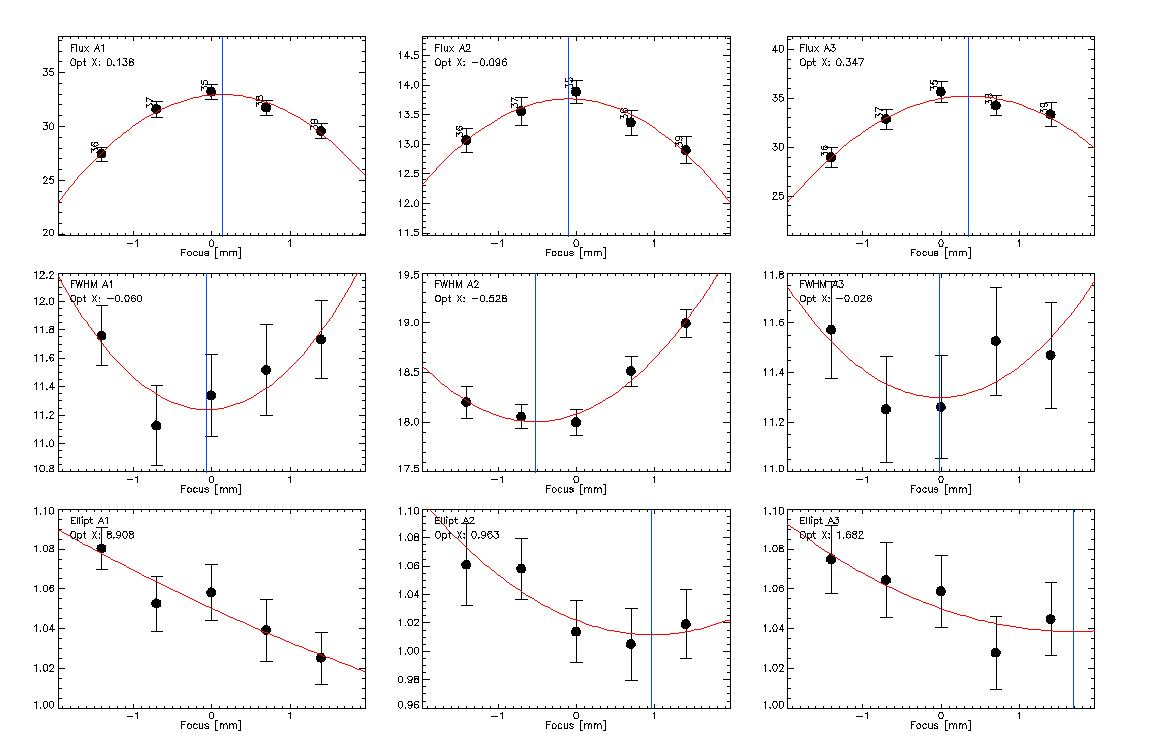
\includegraphics[height=8cm]{Figures/plot_20170223s39.png}
\hspace{0.5cm}
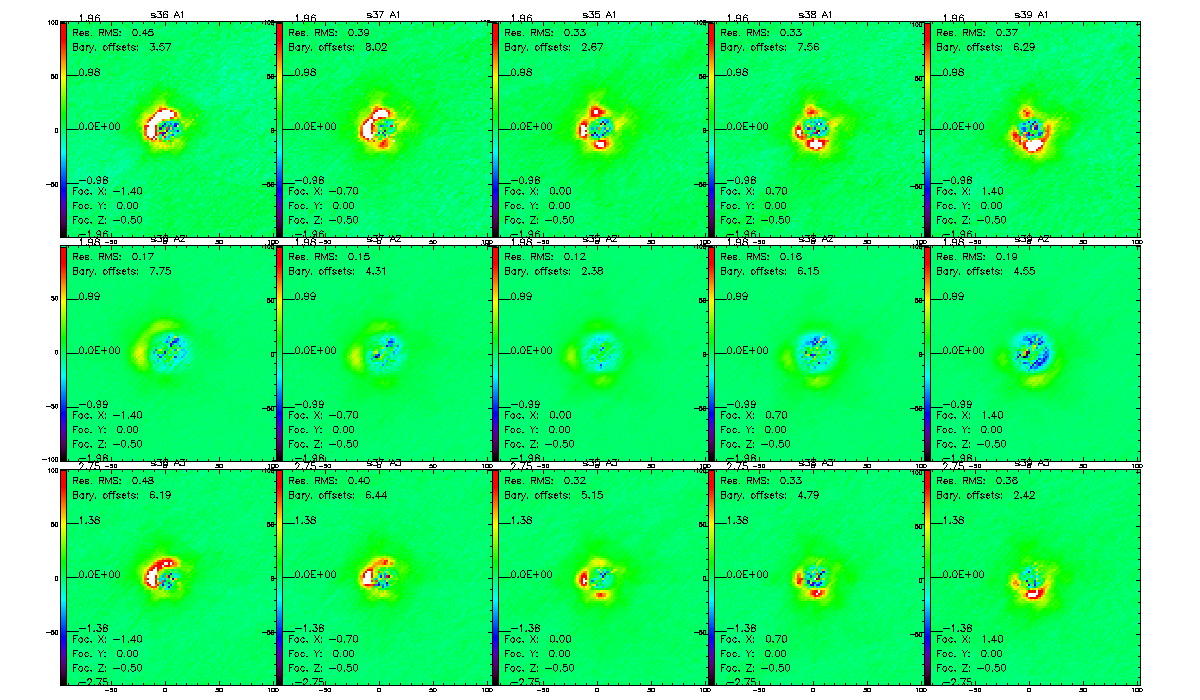
\includegraphics[height=8cm]{Figures/residuals_focus_otf_20170223s39.png}
\caption[Lateral X focus measurements]{\emph{top panel: }X-focus measurement using a
    parabolic fit of the flux, beam FWHM and ellipticity on a sequence
    of five OTF scans on Uranus (20170223s39-43) \emph{bottom panel: }Beam residuals
    after subtracting a model of the main beam for each OTF-scan of the X-focus
    session. (N2R9)}
\label{fig:X_focus}
\end{figure*}

\begin{figure*}[h!]
\centering
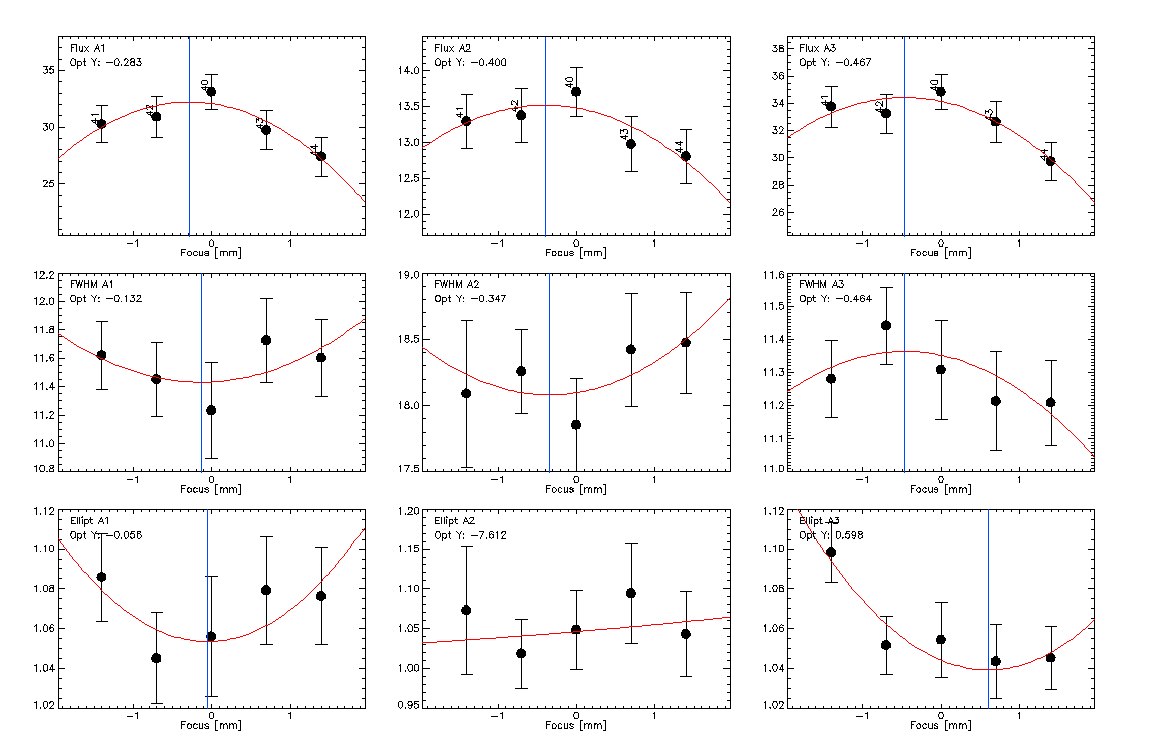
\includegraphics[height=8cm]{Figures/plot_20170223s44.png}
\hspace{0.5cm}
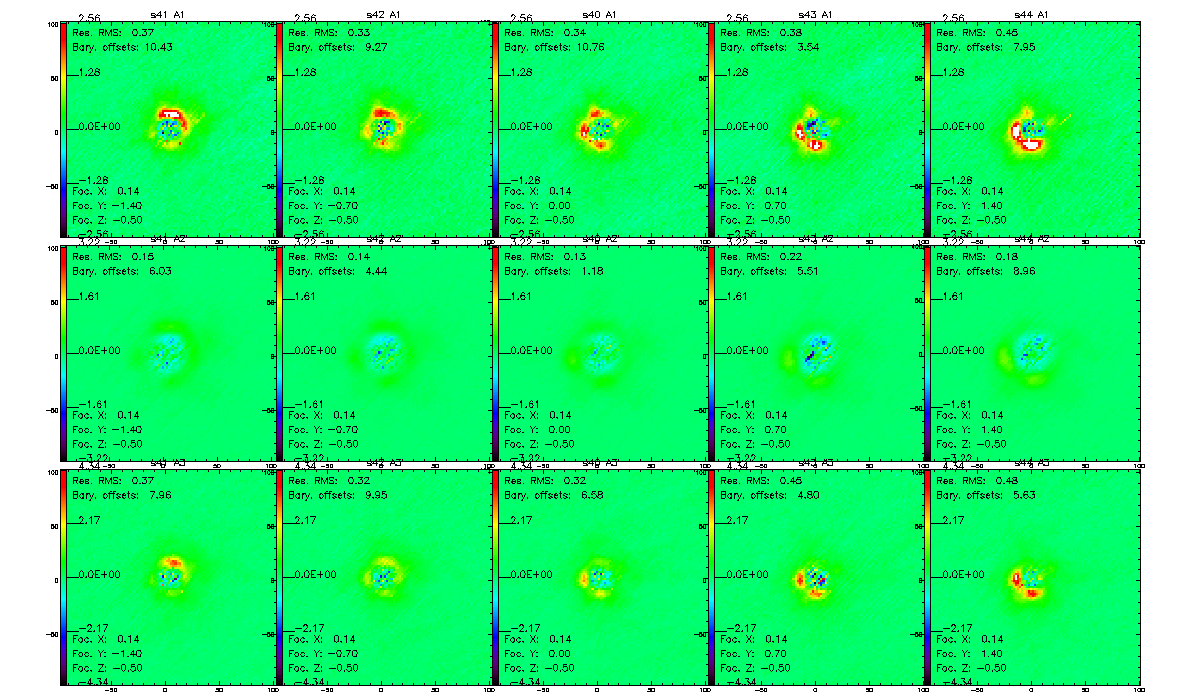
\includegraphics[height=8cm]{Figures/residuals_focus_otf_20170223s44.png}
\caption[Lateral Y focus measures]{\emph{top panel: }Y-focus measurement using a
    parabolic fit of the flux, beam FWHM and ellipticity on a sequence
    of OTF scans on Uranus (20170223s44-48). \emph{bottom panel: }Beam residuals
    after subtracting a model of the main beam for each OTF-scan of the Y-focus
    session. (N2R9)}
\label{fig:Y_focus}
\end{figure*}


\subsection{Pointing}
\label{se:pointing}
% + RTA pointing estimate method
% + pointing model
% + pointing error (scan-to-scan scattering)

Once the instrument is correctly focused, we can estimate pointing corrections
before scientific observations.
%The procedure that is used is very similar to
%that used for EMIR and is described in the next subsection.
\vu{Even though EMIR only has a single pixel on the sky, the pointing procedure
used for NIKA2 is very similar and is described in the next subsections.}
%It was used
%repeatedly during pointing sessions to derive the pointing model of.

\paragraph{Pointing monitoring}

\begin{figure}[ht!]
\begin{center}
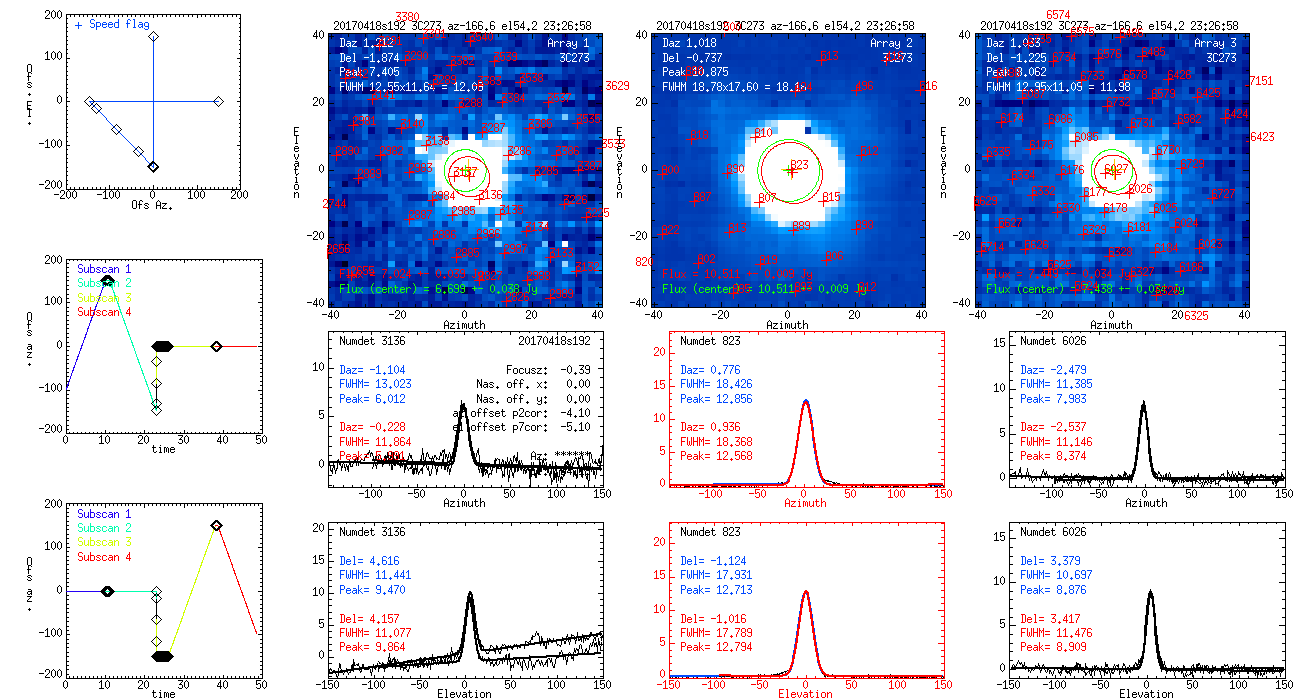
\includegraphics[clip, angle=0, scale = 0.30]{Figures/plot_20170418s192.png}
\caption[Summary plots of the reduction of pointing scan.]{Top plots
  show the combined map for array 1, 2 and 3, which enable a check of
  the overall quality of the scan, while bottom plots show the set of azimuth
  and elevation profiles for one reference detector per array. The
  reference detector per array is highlighed with a red cross in the
  centre of the map. The pointing reference detector of
  \nika\ is the 2\,mm reference detector, the azimuth
  and elevation profiles of which are shown in the central bottom
  plot. The location of the peak in azimuth and elevation, as observed by the
  reference detector gives the pointing offsets of the current scan.
}
\label{fig:ptg}
\end{center}
\end{figure}

\begin{figure}[ht!]
\begin{center}
\includegraphics[clip, angle=0, trim={0, 0, 3cm, 0}, width=0.65\textwidth]{Figures/pointing_stats_N2R9.eps}
\caption[Pointing session results]{Pointing offsets during Run9 observations,
  before (blue to green) and after (yellow to red) the
  derivation of Nasmyth offsets with a pointing session on Feb.~26th, 2017.}
\label{fig:pointing_stats_n2r9}
\end{center}
\end{figure}

Based on general operating experience at the 30\,m telescope, we use the so-called
{\em pointing} or {\em cross} scans to monitor the pointing during observations. The
telescope executes a back and forth scan in azimuth and a back and forth scan in
elevation, centered on the observed source. Looking at the timeline profiles of
the reference detector, we fit gaussian profiles and derive the current pointing
offsets of the system in azimuth and elevation. These offsets can then be passed
to PAKO to recenter the next scan (Fig.~\ref{fig:ptg}).

\paragraph{Pointing session}
\label{se:pointing_session}

Such scans and their analyses are also used to improve the pointing model of
\nika. A pointing session consists in observing about 30 sources on a wide range
of elevations \new{and azimuth angles} while monitoring the pointing offsets
that are measured for each observation. These offsets are then passed to the
IRAM staff who finds the pointing model parameters that minimize and symmetrize
the scattering of these offsets. Based on these results, the Nasmyth offsets
parameters that enter the IRAM pointing model are
adjusted. Fig.~\ref{fig:pointing_stats_n2r9} shows the pointing corrections that
had to be applied during Run9, before and after the modification of the Nasmyth
offsets. The dispersion of the offsets is the figure of merit of the pointing
corrections. Their distribution after the corrections (in yellow to red) is
clearly more symmetric and narrower than before. During N2R9 run, \vu{the rms of
  the residual scatter after the
  correction} was 1.62\,arcsec rms in azimuth and 1.37\,arcsec rms in elevation.

\subsection{Skydip}
\label{se:skydip}

A {\tt skydip} scan \new{with NIKA2} consists in a step-by-step span
of a large range of elevations. This is used in order to calibrate the
KIDs response to the atmosphere for opacity derivation, as discussed in
Sect.~\ref{se:opacities}.
\new{Whereas with the heterodyne receivers, skydips can be
  conducted continuously slewing the telescope in elevation, this
  option is not feasible with NIKA2, as the KIDs need to be retuned
  for a given airmass.}
For that purpose, a NIKA2 skydip comprizes eleven steps in
the elevation range from 19 to 65 degrees, regularly spaced in
airmass. For each step, we acquire about twenty seconds of time traces
to ensure a precise monitoring of each KIDs. KIDs are tuned at the beginning of
each subscan (hence once per airmass). The variation of their resonance
frequency reads

\begin{equation}
  %\ftone^k  = C_0^k - C_1^k T_{atm}[1-e^{-\tau/\sin\delta}]
  f_{\rm{reso}}^k  = C_0^k - C_1^k T_{atm}[1-e^{-\tau/\sin\delta}]
\label{eq:skydip_1}
\end{equation}

An illustration is presented on Fig.~\ref{fig:ftone_vs_elev}. More details on
the analysis of these {\tt skydip} scans are given in Sect.~\ref{se:opacities}.

\begin{figure}[ht!]
\begin{center}
  \includegraphics[clip, angle=0, scale=0.75]{Figures/skydip_report.eps}
\caption[skydip]{Variation of the resonance frequency of a KID
  \new{$f_{\rm{reso}} = \ftone + \delta \ftone$},  as a function of the
  elevation during a {\tt skydip} scan.}
\label{fig:ftone_vs_elev}
\end{center}
\end{figure}

\subsection{\bms}
\label{se:beammaps}

A \bm\ is \vu{a scan procedure to map} a bright and compact
source, most of the time a planet, with
an elevation step small enough to meet Nyquist sampling of the 1\,mm beam,
namely 4.8~arcsec. We observe the planet with a raster scan in (az,el)
coordinates of $13\times7.8$~arcmin$^2$, either with fixed elevation subscans or
fixed azimuth subscans. The former has the advantage of low air mass variation
across a subscan, the latter offers an orthogonal scan direction to the former:
the combination of both gives a more accurate determination of the far side
lobes. The scan size ensures that the entire FOV is observed with good margins
for beam mapping even on the edges and good margins for baseline derivation and
subtraction in the scanning direction. During subscans, the telescope travels at
65\,arcsec/s. This value results of a tradeoff between the need to scan as
fast as possible to minimize atmospheric contamination and the
necessity to keep subscans no shorter than 10\,s (telescope
constraint). The need to have Nyquist sampling of
the beams along the scan direction translates into a maximum speed of 110\,arcsec/s
for our nominal acquisition rate of 23.8\,Hz and is thus largely met. Subscans
last 12\,s, the entire scan lasts about 25\,min, which is short enough to prevent
%too much variation of KID tuning under stable weather conditions on
%this timescale.
\sam{losing the signal due to atmosphere-induced (1/f) background variations that would
  move the resonance away from the tone probing it.}


More details on these observations are given in Sect.~\ref{se:fp_reconstruction}
where we describe how to actually exploit them to derive individual KID
properties.


%%	CALIBRATION PIPELINE, DATA REDUCTION, DATA SELECTION
%\section{Data reduction: from timelines to maps {\color{blue} Nico et al.} }
%\label{se:toi2maps}



\subsection{Data selection}% {\color{YellowGreen} Laurence}}
\label{se:data_selection}

For calibration and performance assessment, we select scans in average
observing conditions by performing mild selection cuts. These scan
cuts rely on zenith opacity estimates in NIKA2 bands $\tau$, as
described in Sect.~\ref{se:opacities}, and on the observation date
conditions where:
%
\begin{itemize}
\item[i)] $\tau_{3} < 0.5$, where $\tau_{3}$ is the $\tau$ estimate for
  Array 3, corresponding to a decrease of the signal by a factor of
  two at $45^{o}$ of elevation;
\item[ii)] $x\, \tau_{3} < 0.7$ and $\elev > 20^{o}$, where $\elev$ is the
  elevation of the telescope and $x$ the
  air mass, which depends on the elevation as $x=(\sin{\elev})^{-1}$. This
  threshold corresponds to a decrease of the signal by a factor of two;
\item[iii)] observation date from 22:00 to 9:00 UT and from 10:00 to
  15:00, that is excluding the sunrise period and the late afternoon.
\end{itemize}
%
As discussed in Sect.~\ref{se:obsdate_variations}, the late afternoon
observation are often affected by telescope-driven beam broadening. Around
sunrise, the focus shifts continuously due to the ambient temperature
change until the temperature stabilizes, so that the scans taken from
9:00 to 10:00 UT are likely not to be optimally focused.
After the focus stabilisation, morning period 
from 10:00 to 15:00 UT offers stable observing conditions
if the telescope is not heated due to observations in a
direction close to the Sun. Otherwise, further scan selection based \new{on
the exact sequence of observations and on beam monitoring} might be needed before using these
observations for performance assessment.

   
In addition to the above scan selection cuts, we use a Gaussian beam
size criterion for the absolute calibration on planets
(e.g. Uranus). Namely, the FWHM estimated from the planet observation
map is asked to be lower than $12.5''$ at $1\,\rm{mm}$ and lower than $18''$ at
$2\,\rm{mm}$. In further mitigating the flux scatter due to beam broadening, we
ensure better accuracy of the absolute calibration.  
%, which correspond to a beam about $15\%$ larger than the average
%beam (see Sect.~\ref{se:beams}). The rational of this extra cut is
%mitigating the flux scatter due to beam broadening, and thus
%preserving the absolute calibration accuracy, as discussed in
%Sect.~\ref{se:calibration}.






\clearpage
%----------------------------------------------------------------------------------------
%	OPACITY
%----------------------------------------------------------------------------------------
\chapter{Opacity derivation}% {\color{YellowGreen} Laurence et al.}}
\label{se:opacities}
%----------------------------------------------------------------------------------------
%	OPACITY METHODS
%----------------------------------------------------------------------------------------
%\section{Opacity derivation}
%\label{se:opacities}
%
% LP: copie de l'intro de Xavier
In NIKA2, the opacity is measured via a total-power technique, which was successfully tested with NIKA. The details of this technique and its agreement with the Atmospheric Transmission at Microwaves (ATM) model (\cite{2001IEEE....49.1683C}) are described in \cite{Catalano2014}. The underlying idea is to replace the opacity, usually delivered by the resident IRAM tau-meter that performs elevation scans at a fixed azimuth and is operating at 225\,GHz, by a measurement that uses the NIKA2 instrument itself as a tau-meter. Using this procedure we can directly derive an opacity integrated in the NIKA2 very bandpasses and in the same line-of-sight of the source in the considered map. First, we have to calibrate the relationship between total power and opacity.
% fin copie

\subsection{Methodology}
For each kid $k$, the absolute value of the resonance frequency
$f_{tone}^k$ moves with the atmospheric load according to

\begin{equation}
f_{tone}^k = C_0^k + C_1^k T_{atm}[1-e^{-\tau/\sin\delta}]
\end{equation}

{\bf LP: pourquoi signe plus alors qu'on utilise un signe moins dans
  Eq. 2 du papier instru ?}

where $C_0^k$ is a constant equal to the resonance
frequency at zero opacity, $C_1^k$ is the calibration conversion
factor in kHz$/$K, $T_{atm}$ is the equivalent temperature
of the atmosphere (taken as a constant at 270K), $\tau$ the zenith
opacity and $\delta$ the average elevation of the telescope.
By assuming a homogeneous plane-parallel atmosphere, the airmass $x$ is defined from the
elevation as $x = \sin\delta$. 

The coefficients $C_0^k$ and $C_1^k$ are expected to be constant in time
within at least a cooldown cycle, and are determined using a {\tt
  skydip} procedure. This consists in moving
the telescope in elevation step by step and to monitor, for each kid, the
evolution of $f_{tone}^k$ vs the air mass and to fit the zenith opacity $\tau$ and
$C_0^k$ and $C_1^k$. Namely, during a {\tt skydip}, the telescope performs
eleven elevation steps in the elevation range from 19 to 65 degrees, regularly
spaced in airmass. For each step, we acquire about twenty seconds of
time traces to reduce the error in the determination of $f_{tone}^k$.

All the skydips (that were obtained under various opacity
conditions) are analysed together to break the degeneracies between
the opacity and the responsivity. The procedure has two steps.
First, all the skydips are analysed individually to simply measure
$f_{tone}^k$ for each stable elevation and fit simultaneously all the
parameters ($\tau$, $C_0^k$ and $C_1^k$.)
Error bars on $\tau$ are estimated by doing
this procedure on blocks of 40 kids only and getting a dispersion on the
resulting $\tau$ from the different blocks. Usually the dispersion comes out as
$4\times 10^{-3}$ at 1mm and $1\times 10^{-3}$ at 2mm. Once the $\tau$ values
are estimated for each skydip (as the average over the blocks), we compute
(while fixing $\tau$) the $C_0$ and $C_1$ final values for each KID. We thus
retrieve the coefficients of all the KIDs even though some of them could not
contribute to the tau determination.

%% \begin{figure}
%% \begin{center}
%% 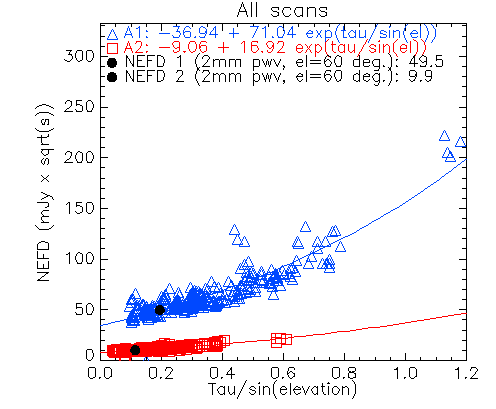
\includegraphics[clip, angle=0, scale =
%%   0.5]{Figures/NEFD_vs_tau_20170226s415_FXDC0C1_Jy_common_mode_kids_out.png}
%% 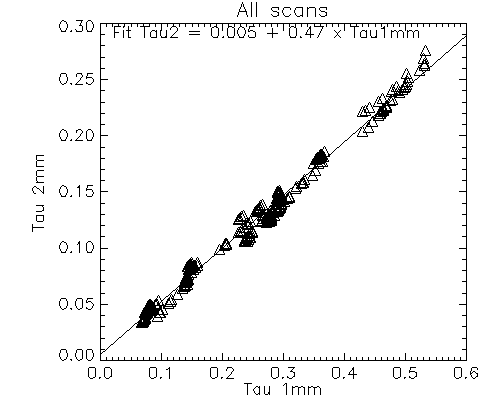
\includegraphics[clip, angle=0, scale =
%%   0.5]{Figures/tau1_tau2_20170226s415_FXDC0C1_GaussPhot_common_mode_kids_out.png}
%% \caption{}
%% \label{fig:fov}
%% \end{center}
%% \end{figure}

%  figure deplacee dans Opacity_checks.tex
%\begin{figure}
%\begin{center}
%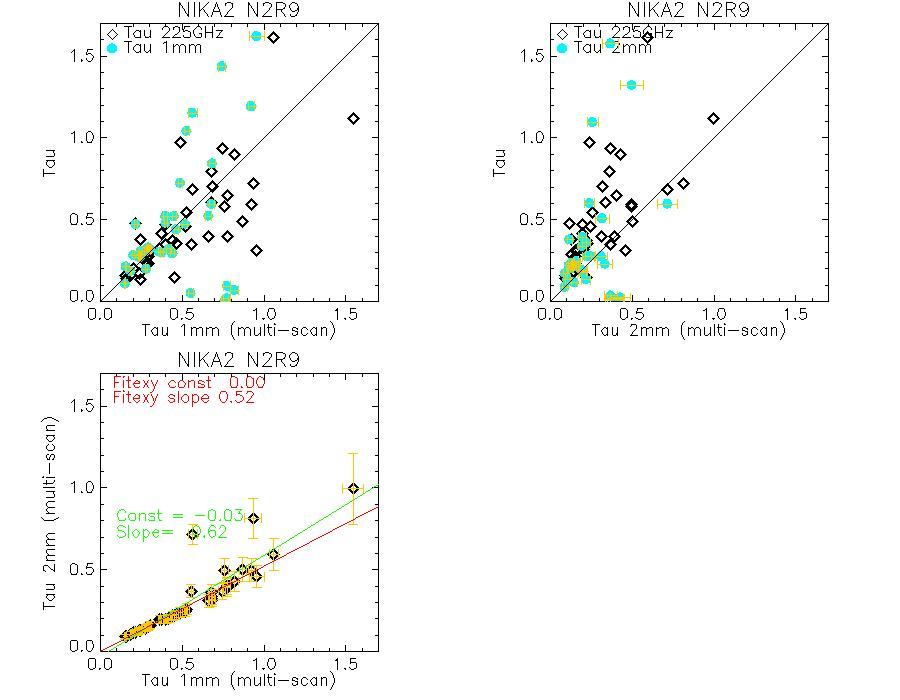
\includegraphics[clip, angle=0, scale = 0.5]{Figures/test_allskd_N2R9.jpg}
%\caption{{\bf Fix me : improve plot quality and plot only the 3rd one.}}
%\label{fig:test_allskd_N2R9}
%\end{center}
%\end{figure}

%\subsection{Opacity measurement consistency tests}

%{\bf copy from the 'Instru' paper}

\begin{figure}[ht]
\begin{center}
\includegraphics[scale=0.8]{Figures/test_allskd_N2R10v2commiss2.pdf}
\caption{Atmospheric opacity as measured from the NIKA2 data 
at 260 (top) and 150\,GHz (bottom) during N2R10
commissioning campaign. Each block of 40 KIDs gives an independent estimate of
the opacity value for each skydip scan (the integer abscissae). The block
number is the decimal value of the abscissae.
\label{fig:taumeas_paper}}
\end{center}
\end{figure}

\begin{figure}[ht]
\begin{center}
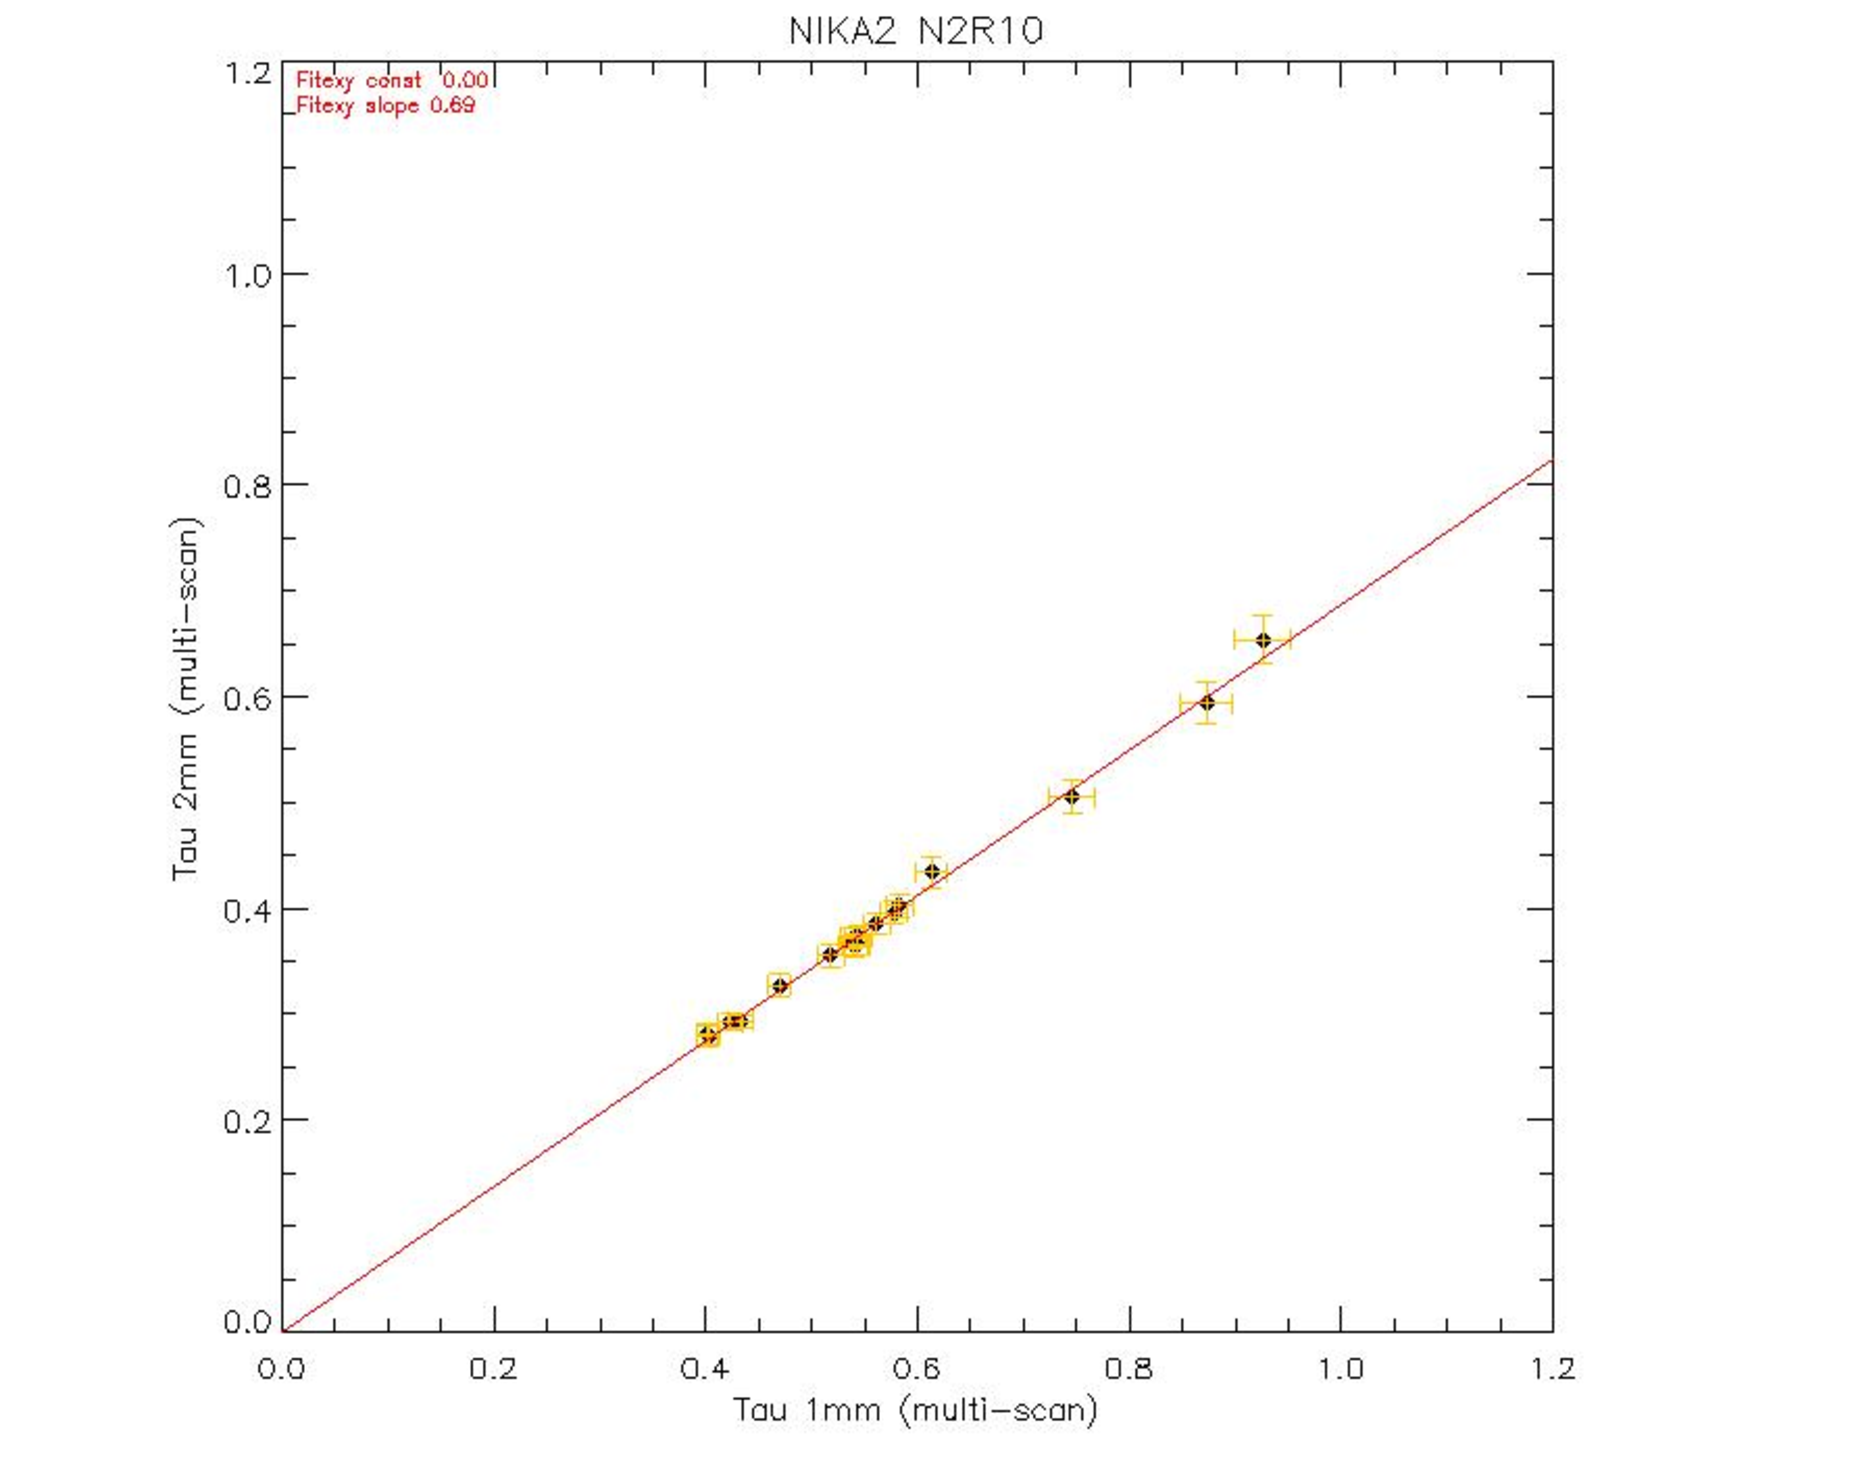
\includegraphics[scale=0.8]{Figures/test_allskd_N2R10v2commiss1.pdf}
\caption{Atmospheric opacity as measured from the NIKA2 data 
at 260 and 150\,GHz during N2R10
commissioning campaign. The error bars are in fact dispersion of the deduced
opacities between blocks of 40 KIDs.
\label{fig:taumeas_paper}}
\end{center}
\end{figure}

We observe that the skydip-fitted $\tau$ values are, as expected, common
between different detectors of the same array (the two 1mm arrays show
slightly different values). By comparing the results of different skydips, we
have verified experimentally that the coefficients $C_0$, $C_1$ are stable,
within the fit errors, on very long time scales within a cooldown cycle. The
coefficients can thus be applied to the whole observing campaign in order to
recover the opacity of each scan.


% \noindent {\bf FM : a figure would help to convince the reader that it is stable on lng time
% scale, which is a key point.}\\ FXD: I will do that figure


\begin{figure}[ht]
\begin{center}
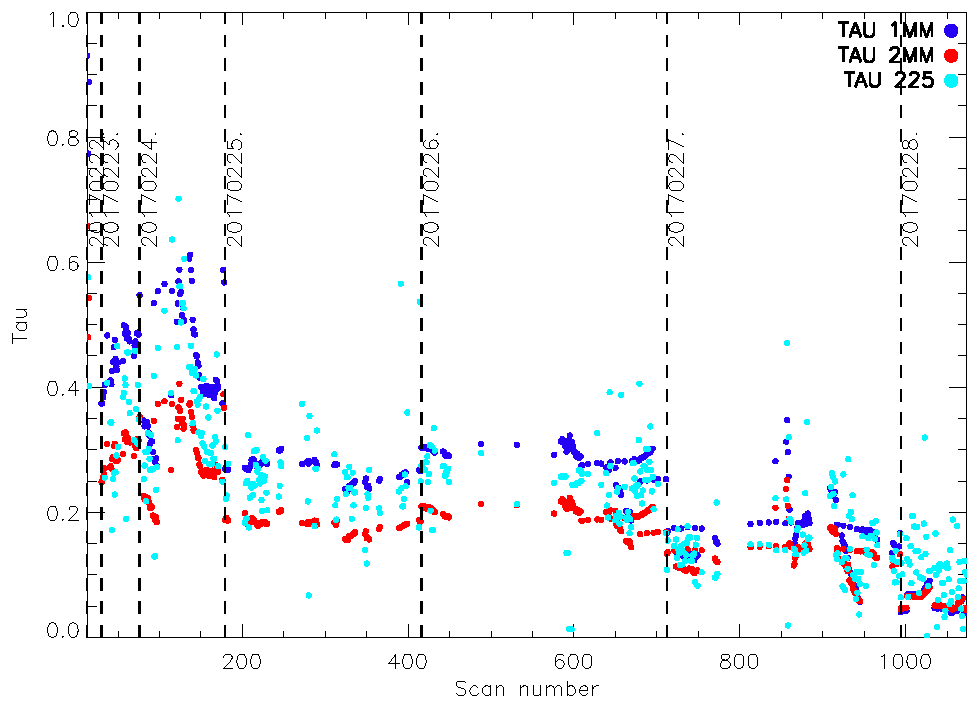
\includegraphics[scale=0.8]{../../Paper_NIKA2_Technical/opacity_evol_run22.pdf}
\caption{Atmospheric opacity as measured from the IRAM 225\,GHz taumeter
(cyan), and from the NIKA2 data at 150 (red) and 260\,GHz (blue) during N2R9
commissioning campaign (Feb. 2017). We stress the fact that the IRAM 225\,GHz
taumeter data is not used for the atmospheric correction and is plotted here
just for comparison.
  \label{fig:taumeas_paper}}
\end{center}
\end{figure}


\begin{figure}[ht]
\begin{center}
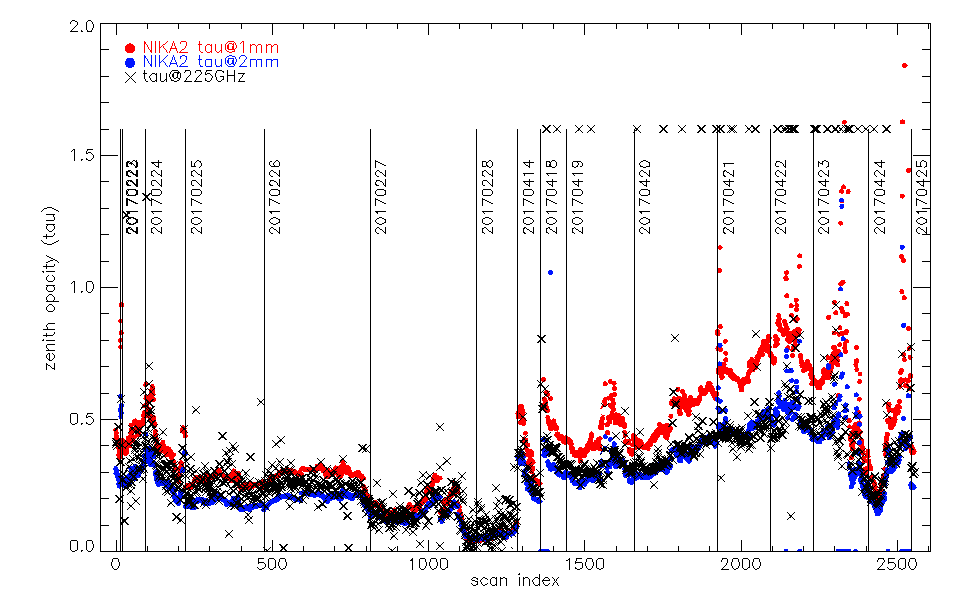
\includegraphics[width=\linewidth]{Figures/opacity_vs_index_N2R9_N2R10.png}
\caption{Atmospheric opacity as measured from the IRAM 225\,GHz
  taumeter (black crosses), and from the NIKA2 data at 150 (red) and 260\,GHz (blue) during 
  N2R9 and N2R10 commissioning campaigns.  We stress the fact that the IRAM 225\,GHz taumeter data is not used for the atmospheric correction and is plotted here just for comparison.
  \label{fig:taumeas}}
\end{center}
\end{figure}


In Fig.~\ref{fig:taumeas} {\bf(and Fig.~\ref{fig:taumeas_paper} of
  \ref{NIKA2-Tech}) } we present the evolution of the NIKA2 in-band
opacities for all the 'OTF' scans (about 1300 scans per runs) of the
N2R9 run held in February and the N2R10 run in April 2017. These are
compared to the IRAM tau-meter values. We observe an agreement on the global trend between the IRAM tau-meter opacity
(225 GHz) and the NIKA2 values. These latter show, however,
a smaller dispersion (less than one percent).
% {\bf FM : how small ?}.


We find an average ratio between the 150 GHz and the 260 GHz NIKA2 values of
about 0.6, a bit higher than ATM model expectations. We notice however that
the 150 GHz-to-260 GHz opacity ratio varies significantly for opacities (at
150 GHz) below 0.2. This effect is likely to be linked to an $O_2$ atmospheric
line which becomes saturated or to some spillover at 2mm. This point is,
however, still under investigation.''


% \noindent {\bf FM : a figure of the ratio of taus would be useful. It should be compared with  
% Fig. \ref{thopacities}, which should appear in this section ...}
% FXD: figure above gives the measured ratio. 


\begin{figure}[ht]
\begin{center}
  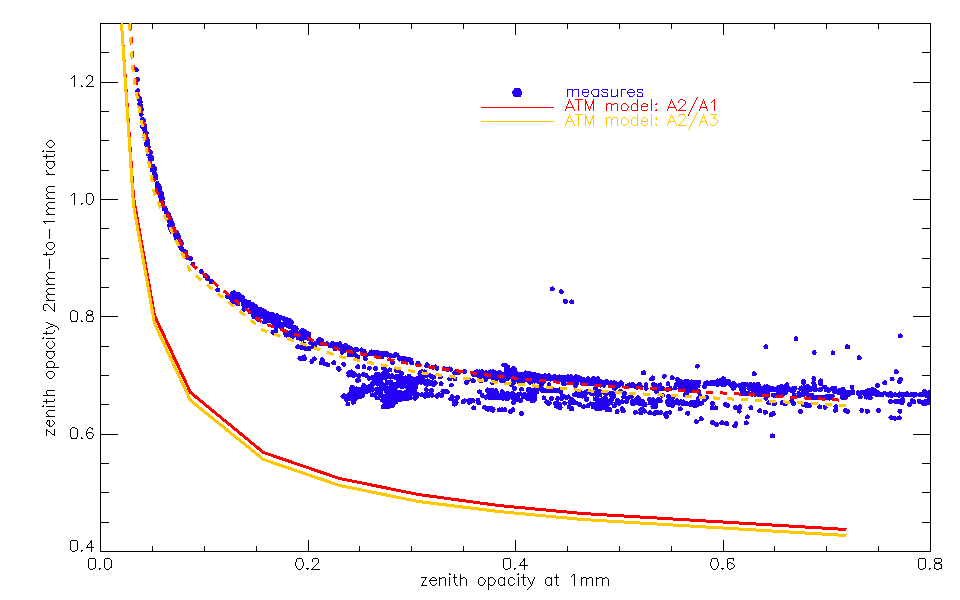
\includegraphics[width=0.65\textwidth]{Figures/opacity_tau1_tau2_ratio_N2R9_N2R10.png}
  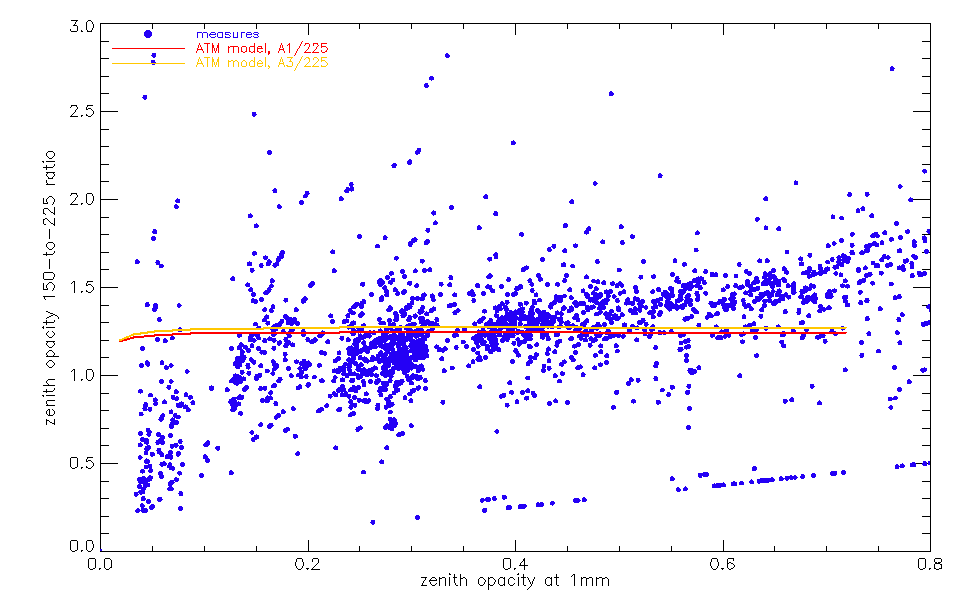
\includegraphics[width=0.65\textwidth]{Figures/opacity_tau1_tau225_ratio_N2R9_N2R10.png}
  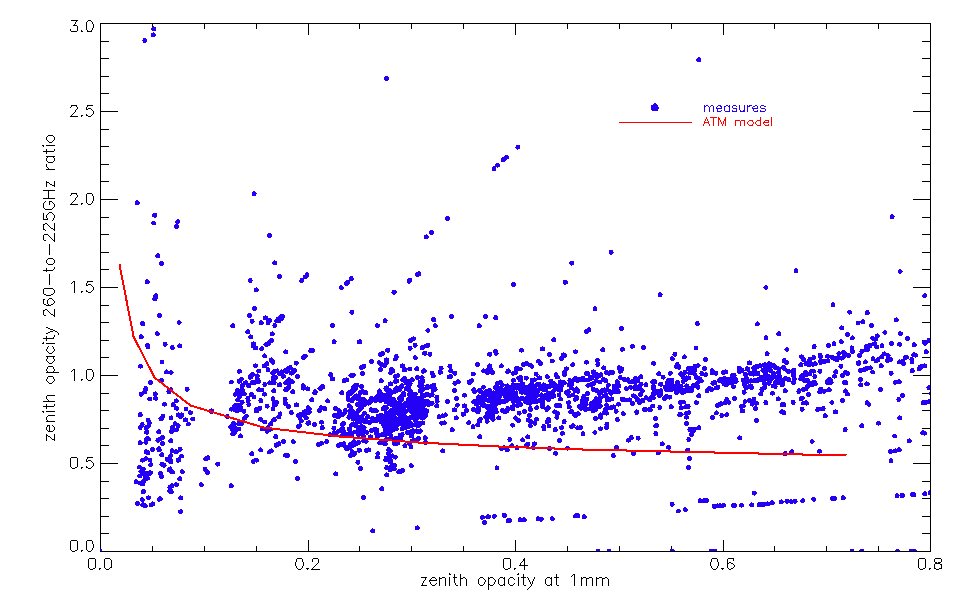
\includegraphics[width=0.65\textwidth]{Figures/opacity_tau2_tau225_ratio_N2R9_N2R10.png}
\caption{Ratios between the 150 GHz and the 260 GHz NIKA2 zenith opacity
estimates and between the NIKA2 $\tau$ and the IRAM taumeter
values. The expectation values derived for NIKA2 bands
using the ATM model described in \ref{Pardo2002} are shown for
comparison (red and orange curves).}
  \label{fig:opacity_ratios}
\end{center}
\end{figure}

\begin{figure}[ht]
\begin{center}
  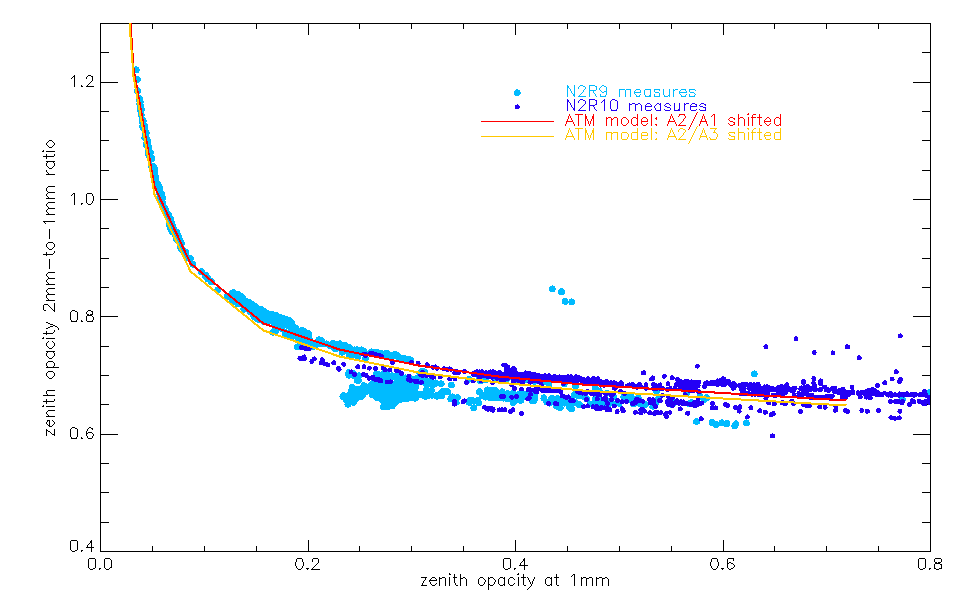
\includegraphics[width=0.8\textwidth]{Figures/opacity_tau1_tau2_byrun_ratio_N2R9_N2R10.png}
  \caption{Ratio between the 150 GHz and the 260 GHz NIKA2 zenith opacity
estimates. The expectation values derived for NIKA2 bands
using the ATM model described in \ref{Pardo2002} are shown for
comparison (red and orange curves). The observed NIKA2 opacity ratio
has a smooth, consistent behaviour over the overall probed opacity range,
and very few outlier estimates are seen although no scan selection has
been performed (out from discarding the dark tests). Also remarkable
is the consistency between estimates obtained during two campaigns
held two months apart in different weather conditions (good to average
during N2R9 and poor and often hightly unstable conditions during
N2R10). Some sub-structures are seen in the opacity ratio, which are
under investigations. They can have several origins (telescope cabin
temperature variation, variation of the $0_2$ fraction, atmospheric
temperature variation, internal temperature variations, etc).  
  }
  \label{fig:opacity_ratio_perrun}
\end{center}
\end{figure}


\begin{figure}[ht]
\begin{center}
  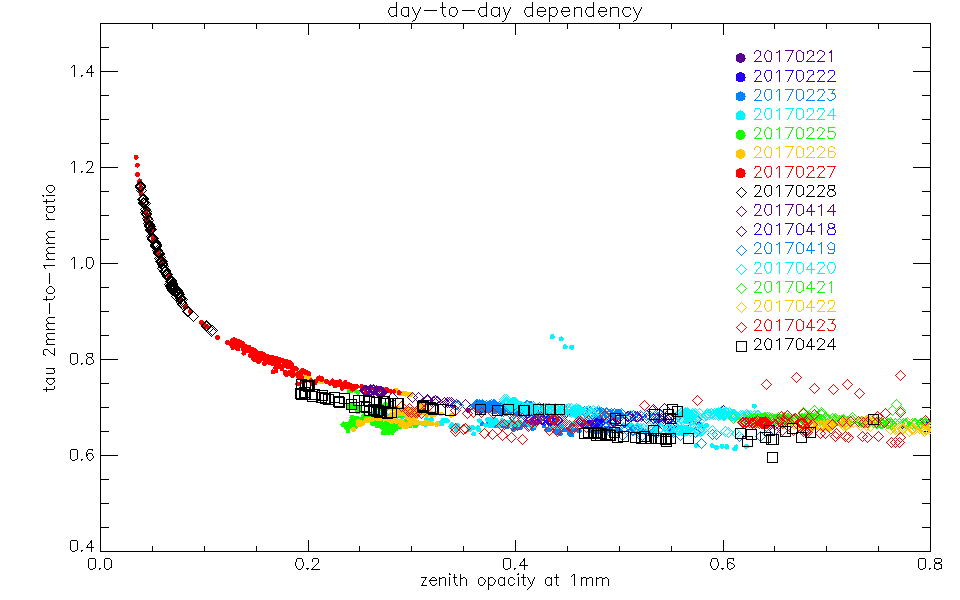
\includegraphics[width=0.8\textwidth]{Figures/opacity_tau1_tau2_ratio_perday_N2R9_N2R10.png}
  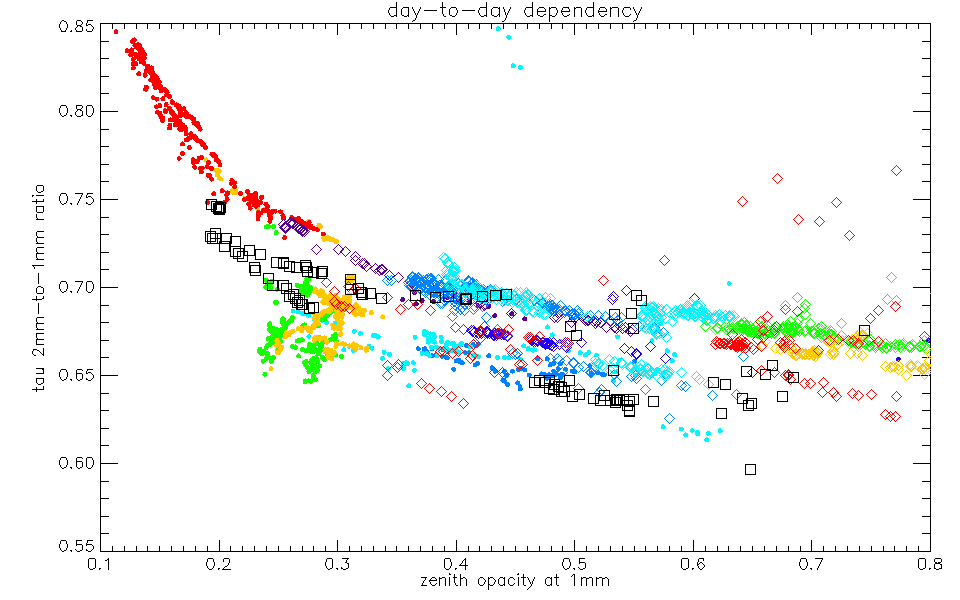
\includegraphics[width=0.8\textwidth]{Figures/opacity_tau1_tau2_ratio_perday_zoom_N2R9_N2R10.png}
  \caption{Ratio between the 150 GHz and the 260 GHz NIKA2 zenith
    opacity estimates. The 4 outlier estimates on February, 24 (in
    cyan) correspond to a test using the external
    calibrator. Different regimes are seen on the 25th and 26th of
    February, while the weather conditions were too unstable to allow
    the astronomer team to focus.
  }
  \label{fig:opacity_ratio_perday}
\end{center}
\end{figure}


\begin{figure}[ht]
\begin{center}
  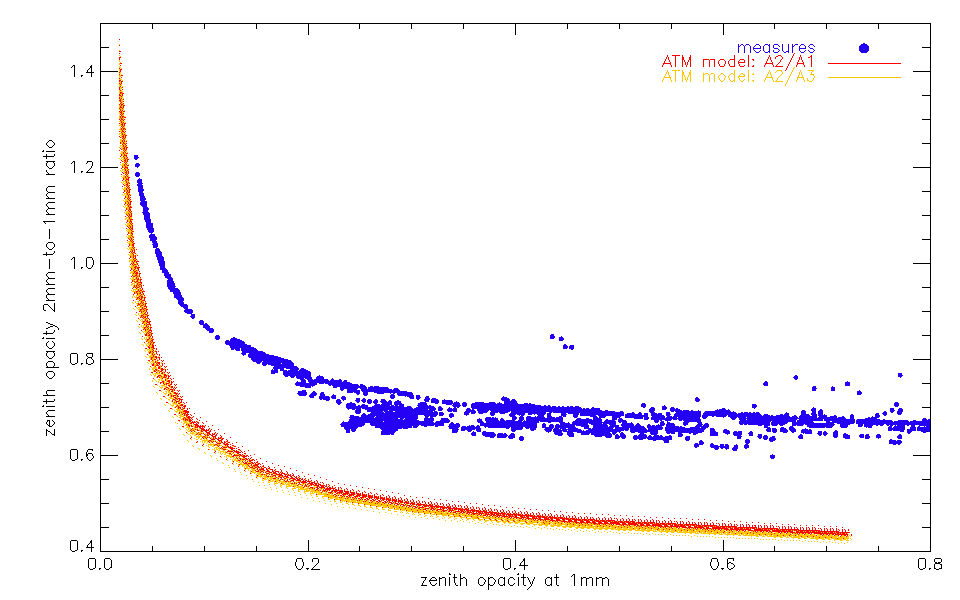
\includegraphics[width=0.8\textwidth]{Figures/opacity_tau1_tau2_ratio_bperror10pc_N2R9_N2R10.png}
  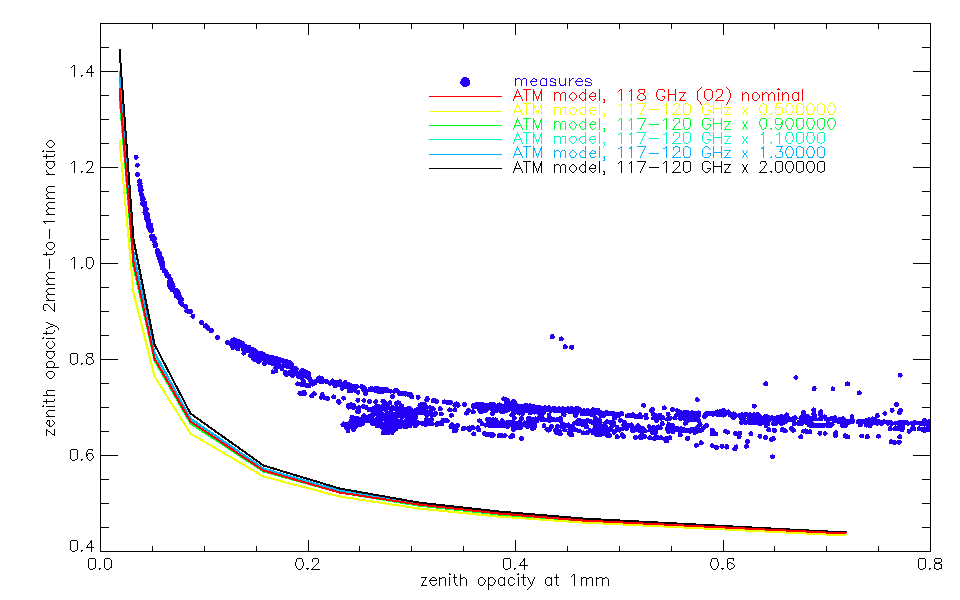
\includegraphics[width=0.8\textwidth]{Figures/opacity_tau1_tau2_ratio_o2fraction_N2R9_N2R10.png}
\caption{Uncertainty of NIKA2 $\tau$ values. Upper panel: The impact
  of the NIKA2 transmission measurement uncertainties is illustrated
  using a very pessimistic relative uncertainty of $10\%$ (instead of
  the more realistic $1\%$ errors). Lower panel: The impact of the
uncertainty on the atmospheric absorption around $118\, \rm{GHz}$, due
to the lack of precise knowledge of the fraction of oxygene in the
atmosphere. The nominal absorption predicted by the ATM model is
modified by a factor from 0.5 to 2 in the $117-120\, \rm{GHz}$
frequency band, where the $0_2$ contributions largely dominates the
water vapor ones. }
  \label{fig:opacity_errors}
\end{center}
\end{figure}

\begin{figure}[ht]
\begin{center}
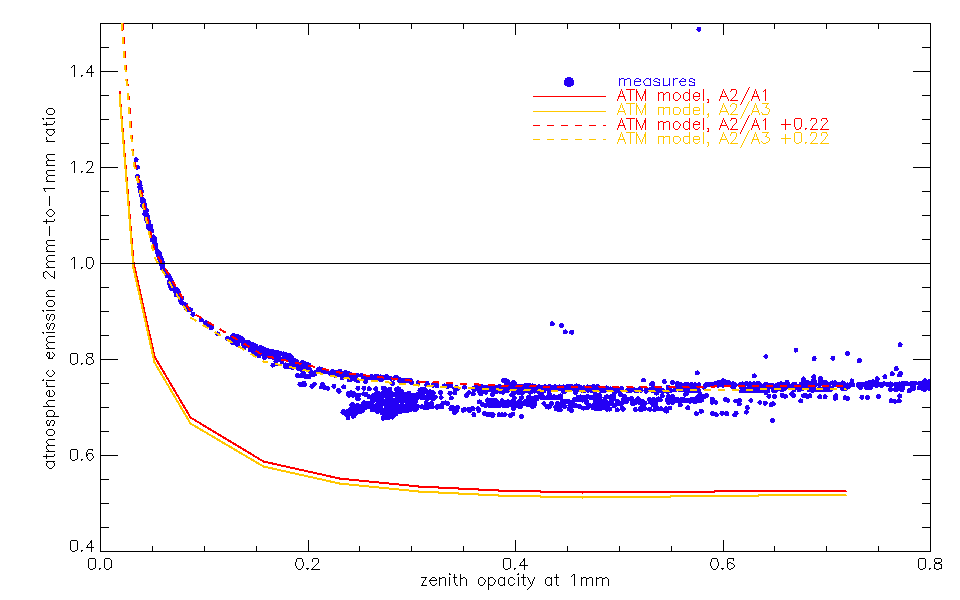
\includegraphics[width=0.9\textwidth]{Figures/opacity_tau1_tau2_emissionratio_N2R9_N2R10.png}
\caption{Ratio of the atmospheric emission in NIKA2 bands defined as
  in Eq.~\ref{eq:opacity_emission_ratio}, compared with the ATM-model
  predicted ratio calculated as in Eq.~\ref{eq:opacity_emission_ratio_model}}
  \label{fig:opacity_emission}
\end{center}
\end{figure}

The ratios between the 150 GHz and the 260 GHz NIKA2 zenith opacity
estimates, quoted $\tau_{2mm}$ and $\tau_{1mm}$ , and
between the NIKA2 $\tau$ and the IRAM taumeter values are presented in
Fig.~\ref{opacity_ratios}, along with the expectation values derived for NIKA2 bands
using the ATM model described in \ref{Pardo2002}. Namely, these
predicted values $\tau^{th}$ are calculated from the ATM-model
atmospheric zenith opacity $\tau^{ATM}$ using:  
\begin{equation}
  \tau^{th}_{A_i} = - \ln{\frac{\int e^{-\tau^{ATM}(\nu)}
      T_{A_i}(\nu) d\nu}{ \int T_{A_i}(\nu) d\nu}},
\end{equation}

where the NIKA2 bandpasses $T_{A_i}$ for arrays $A_i$, $i=1, 2, 3$, are the Martin-Pupplet reference transmissions
corrected by a Rayleigh-Jeans term  $T'_{A_i}(\nu) /
\left( \frac{\nu}{\nu_0}\right)^2$. 

In Fig.~\ref{fig:opacity_emission}, we
show the ratio of the atmospheric emission in NIKA2 bands defined as:
\begin{equation}
  R_{\rm{atm}} = \frac{1-e^{-\tau_{2mm}}}{1-e^{-\tau_{1mm}}}.
    \label{eq:opacity_emission_ratio}
\end{equation}

It is compared with the ATM-model predicted ratio
\begin{equation}
  R_{\rm{atm}}^{th} = \frac{\int (1 - e^{-\tau^{\rm{ATM}}}) T_{A_2}(\nu) d\nu }{\int T_{A_2}(\nu) d\nu} / \frac{\int (1 -
      e^{-\tau^{\rm{ATM}}}) T_{A_{1}}(\nu) d\nu }{\int T_{A_1}(\nu)
        d\nu} .
      \label{eq:opacity_emission_ratio_model}
\end{equation}

In Fig.~\ref{fig:opacity_errors}, we investigate different effects that can impact the precision with
which the zenith opacities are determined: the upper panel shows the
expected dispersion in the NIKA2 $\tau$ values coming from the transmission
measurement uncertainties: to higlight this effect, we consider a very
pessimistic relative uncertainty of $10\%$ (whereas $1\%$ would have
been a more realistic value), and the lower panel shows the impact of the
uncertainty on the fraction of oxygene in the atmosphere, which mainly 
translates in an uncertainty on the atmospheric absorption around
$118\, \rm{GHz}$: the nominal absorption predicted by the ATM model is
modified by a factor from 0.5 to 2 in the $117-120\, \rm{GHz}$
frequency band, where the $0_2$ contributions largely dominates the
water vapor ones. 



We have compared $C_0$ values, the resonance frequency at zero atmosphere,
between different runs. It appears to vary in a systematic manner. For example
we have compared N2R6 and N2R7. The change of frequencies when converted to
temperature (with $c_1$) is of about $25$ and $86$~K at 1 and $2$~mm. This
cannot be a real change of the background. Translated back by a median value
of $c_1$ ($=2500$ and $1500$~Hz/K at 1 and 2 mm), we obtain a 62.5 and 128 kHz
median downward shift of all resonant frequencies between N2R6 (October 2016)
and N2R7 (December 2016). The likely explanation is that of a slight ageing of
the KIDs. A single monolayer of oxyde could be enough to produce the downward
shift.



Only a fraction of the signal is transmitted by the atmosphere and
reaches NIKA2 detectors. 
The relation between uncorrected observed flux densities
$\tilde{S}_{\nu}$ and top-of-the-atmosphere flux densities $S_{\nu}$
is parametrized from the zenith opacity $\tau_{\nu}$
and the line-of-sight airmass $x = \left(\sin\delta\right)^{-1}$ ($\delta$ is the elevation), such as
\begin{equation}
\tilde{S}_{\nu} = S_{\nu} \, e^{-\tau_{\nu}  x}.
\label{eq:uncorr_flux}
\end{equation}

An accurate derivation of the opacity condition for each scan is
required in order to retrieve the source signal at the top of the
atmosphere. Opacity correction uncertainties even prevail in the
final calibration error budget (see Chapter~\ref{se:error}).

We developped three opacity derivation methods, which are discussed in
the sections below, and extensively tested their robustness against
observing conditions. The 'taumeter' method discussed in
Sect~\ref{se:taumeter-method} relies on measurements provided by the
resident IRAM tau-meter operated at $225~\rm{GHz}$ and a fit of the
opacity estimates in NIKA2 frequency bands by imposing the flux
density stability against atmospheric conditions. The 'skydip' method
described in Sect~\ref{se:skydip-method} consists in using NIKA2 as a
taumeter (assuming the resonance frequencies are linearly related to
the total power) by resorting to a series of skydip scans, the
selection of which is addressed in
Sect.~\ref{se:skydip-selection}. Finally, the 'corrected skydip'
method presented in Sect.~\ref{se:corrected-skydip} is a modifed
version of the 'skydip' method that minimizes the dependence of the
measured flux density on the opacity.\\


%----------------------------------------------------------------------------------------
%	taumeter Method
%----------------------------------------------------------------------------------------
\section{Taumeter-based method {\color{YellowGreen} Laurence $\&$ Juan}}
\label{se:taumeter-method}

The IRAM 30m falicity is equipped of a resident taumeter, which performs
elevation scans at a fixed azimuth and is operated at 225~GHz, to
monitor the atmospheric opacity.
Time-stamped zenith opacities at $225$~GHz $\hat{\tau}_{225}$ are derived from the
taumeter measures by Dr. Dave~L.~John. Two different $\hat{\tau}_{225}$
estimates are fitted, one relying on a linear model and the other on
an exponential fitting model. The $\hat{\tau}_{225}$ estimates are then
filtered using the cuts $0< \hat{\tau}_{225} <1.2$ and $R^2 > 0.99$, where
$R$ is the correlation coefficient between the two flavours of
$\hat{\tau}_{225}$ estimates. Redundant samples and outliers are removed.

For the NIKA2 analysis we use the linear filtered  $\hat{\tau}_{225}$ data.
The time-stamped $\hat{\tau}_{225}$ estimates, which are sampled about
every 4 minutes, are interpolated to the time of the NIKA2 scans (we
consider the time of the middle of the scan). For crosscheck we also
produce a smooth version of time-stamped $\hat{\tau}_{225}$ data by
filtering with a running median of 7 samples, which is then
interpolated to the NIKA2 scan times.


\begin{figure}[ht!]
  \begin{center}
    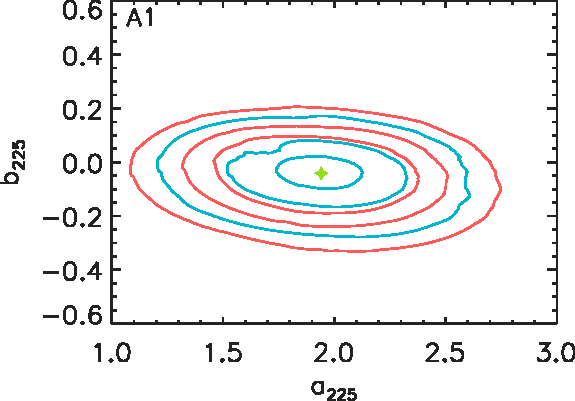
\includegraphics[clip=true, trim={0, -0.3cm, -0.3cm, 0}, width=0.4\textwidth]{Figures/Opacity/fit_nika2_tau_from_taumeter_mwc349_a1.pdf}
    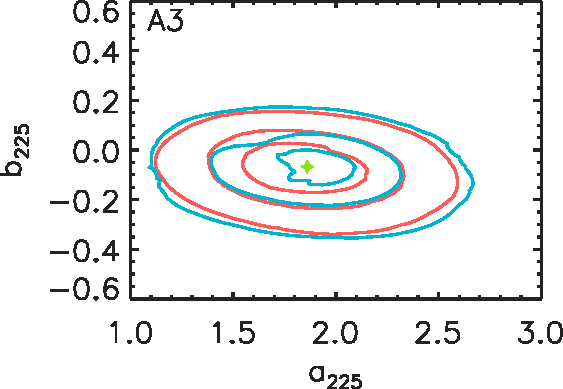
\includegraphics[clip=true, trim={0, -0.3cm, -0.3cm, 0}, width=0.4\textwidth]{Figures/Opacity/fit_nika2_tau_from_taumeter_mwc349_a3.pdf}
    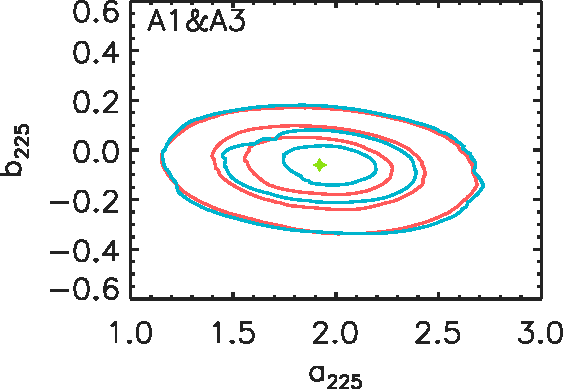
\includegraphics[clip=true, trim={0, -0.3cm, -0.3cm, 0}, width=0.4\textwidth]{Figures/Opacity/fit_nika2_tau_from_taumeter_mwc349_1mm.pdf}
    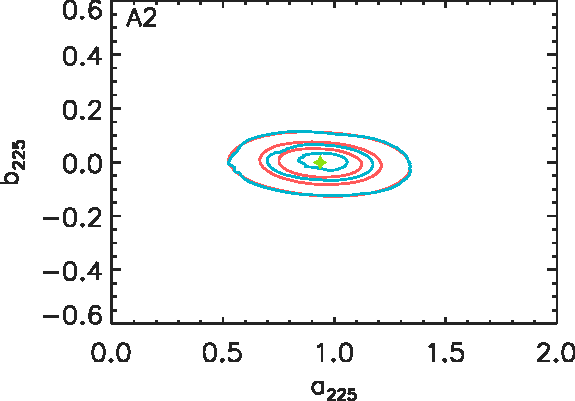
\includegraphics[clip=true, trim={0, -0.3cm, -0.3cm, 0}, width=0.4\textwidth]{Figures/Opacity/fit_nika2_tau_from_taumeter_mwc349_a2.pdf}
    \caption[IRAM taumeter to NIKA2 opacity model]{IRAM $225$GHz taumeter to
    NIKA2 opacity relation fit.
    The $a_{\nu}^{225}$ and
    $b_{\nu}^{225}$ parameter space is explored for Array 1 (upper left),
    Array 3 (upper right), the combination of 1mm arrays (lower left)
    and Array 2 (lower right).
    The red contours correspond to rms
    errors of the measured-to-median flux density ratio of $9\%$, $10\%$
    and $12\%$ at 1mm and $4.5\%$, $5\%$ and $6\%$ at 2mm. The blue
    contours are the $68$, $95$ and $99\%$ confidence
    level contours of the parameters estimated using the $\chi^2$
    minimization.
    The best fit values are shows as green stars} 
\label{fig:taumeter_fit}
\end{center}
\end{figure}

We fit the the relations between the IRAM
$225$GHz taumeter opacities and NIKA2 band pass opacities using
observation of calibration sources which spans a large range of air
masses. We use a series of 64 scans of MWC349, which consists of the
baseline selected sub-set of scans from the 68 available scans for
this source during N2R9.
It constitutes an homogeneous data set in flux density but
heterogeneous in atmospheric conditions: zenith opacities at $225$GHz
range from 0.08 to 0.32 and elevations from $23$ to $73$
degrees, spanning a large range of air mass as required. NIKA2 opacities
$\tau_\nu$, for $\nu$ corresponding
to Array 1, 2, 3 and the combination of Arrays 1 and 3, are estimated
from the $225$GHz taumeter median-filtered exponential-based opacity
estimates $\tau_{225}$ as
\begin{equation}  
  \tau_\nu =  a_\nu^{225}\tau_{225} + b_\nu^{225},          
\end{equation}
where the parameters $a_\nu^{225}$ and $b_\nu^{225}$ are fitted to ensure
that the non-corrected flux densities $\tilde{S}_\nu$ are stable againts
$\tau_{225}$ after correction of the atmospheric attenuation by
inversion of Eq.~\ref{eq:uncorr_flux} using 
\begin{equation}  
  S_\nu = \tilde{S}_\nu e^{(a_\nu^{225}\tau_{225} + b_\nu^{225}) \cdot x}.
  \label{eq:opacorr_taumeter}
\end{equation}

We tested two estimators of the flux stability. The first one relies
on minimising the standard deviation of the measured-to-median flux
densities ratio after correction of the opacity using
Eq.~\ref{eq:opacorr_taumeter}. The second one consists in rewriting
the rms minimisation as an unweighted $\chi^2$ minimisation using:
\begin{equation}
\chi^2 = \sum_{i=1}^{N} \frac{1}{\sigma^2} \, \left( \frac{S_\nu}{Med(S_\nu)} -1 \right)^2,  
\end{equation}
where $\sigma$ is the rms error of the flux density estimates. Note
that these estimators do not depends on
the absolute scale of the flux density of the source.

Figure~\ref{fig:taumeter_fit} show the two flux-stability estimate
contours in the parameter plane ($a_\nu^{225}$, $b_\nu^{225}$), as
well as the best-fitting parameter values. We find
$a^{225} = [1.94,  1.86, 1.92]$ and $b^{225} = [-0.04,  -0.07, -0.06]$
for A1, A3, and the 1mm array combination, while $a^{225}=0.94$ and
$b^{225}=0$ for A2. Uncertainties are of about 0.1 for the $a^{225}$
parameter and about 0.05 on $b^{225}$. 

% bf_a     = 1.9401878      0.94233333       1.8952941       1.9342579
% err_bf_a = 0.16605729     0.097230351     0.084799830      0.12000000
% bf_b     =  -0.045000000       0.0000000    -0.058426966    -0.055000000
% err_bf_b = 0.049497475     0.026340184     0.021199958   0.038890873
%
% -0.043488288  -0.00057861635    -0.060658083    -0.053333333
% 0.050634888     0.027028985     0.022710888     0.040069384
%
%$a = [1.94,  0.94,  1.86,  1.92]$
%$b = [-0.04, 0.00, -0.07, -0.06]$


Because the IRAM tau-meter observes at a fixed azymuth, the
taumeter-based opacities are not exactly the line-of-sight opacities for
the observation scans. As discussed in
Sect.~\ref{se:photometry_others}, this induces larger rms errors of
the top-of-the-atmosphere flux density estimates with respect to
opacity correction methods that relies on skydip-based measurements using
NIKA2 instrument itself. The taumeter-based method will thus be used
as an alternative method in case of failure of the NIKA2 skydip-based
methods and ii) to perform consistency checks.

%{\color{blue} FXD: We could state that the error bars on the coefficients $a$ and $b$ are large and that this method does not measure directly the line of sight opacity, hence we use this method as a backup.}



%----------------------------------------------------------------------------------------
%	skydip-based Method
%----------------------------------------------------------------------------------------
\section{Skydip-based method {\color{YellowGreen} Xavier $\&$ Laurence}}
\label{se:skydip-method}

% LP: copie de l'intro de Xavier
In NIKA2, the opacity is measured via a total-power technique, which was
successfully tested with NIKA. The details of this technique and its agreement
with the Atmospheric Transmission at Microwaves (ATM) model
(\cite{2001IEEE....49.1683C}) are described in \cite{Catalano:2014nml}. The
underlying idea is to replace the opacity, usually delivered by the resident
IRAM tau-meter by a measurement that uses the NIKA2 instrument itself
as a tau-meter. Using this procedure we can directly derive an opacity
integrated in the NIKA2 very bandpasses and in the same line-of-sight of the
source in the considered map. For that purpose, we assume that the resonance
frequency of each KID varies linearly with the total power. First, we have to
calibrate the relationship between total power and opacity. Then we can use
that calibration to measure the opacity during a given scan.
% fin copie

For each KID $k$, the absolute value of the resonance frequency
$f_{reso}^k$ moves with the atmospheric load according to

\begin{equation}
f_{reso}^k  = c_0^k - c_1^k T_{atm}[1-e^{-\tau x}]
\label{eq:skydip}
\end{equation}

%FXD corrected 
%{\bf LP: pourquoi signe plus alors qu'on utilise un signe moins dans
%  Eq. 2 du papier instru ?}

where $c_0^k$ is a constant equal to the resonance frequency at zero
opacity, $c_1^k$ is the calibration conversion factor in Hz$/$K,
$T_{atm}$ is the temperature of the atmosphere (taken as a constant at
270~K, we therefore neglect the atmospheric temperature variations),
$\tau$ the zenith opacity and $\delta$ the elevation of the
telescope.  By assuming a homogeneous plane-parallel atmosphere, the
airmass $x$ is defined from the elevation as $x
= \left(\sin\delta\right)^{-1}$ (we neglect the Earth sphericity).

The coefficients $c_0^k$ and $c_1^k$ are expected to be constant in
time within at least a cooldown cycle (because the coupling of NIKA2
to the telescope does not change), and are determined using a {\emph
skydip} procedure. This consists in moving the telescope in elevation
step by step, that is, performing a skydip scan, as defined
in~Sect.~\ref{se:skydip}, and monitoring, for each kid, the evolution
of $f_{reso}^k$ versus the airmass and to fit the zenith opacity
$\tau$ and $c_0^k$ and $c_1^k$. The acquisition time spent on each
elevation step, which is of about twenty seconds, is chosen to reduce
the error in the determination of $f_{reso}^k$.

All skydips, obtained under various opacity conditions, are analysed
together to break the degeneracy between the opacity and the
responsivity ($c_1^k$). The degeneracy occurs mostly for low opacity
conditions for which we can only determine the combination $c_1^k \tau
x$. The procedure has two steps.  First, all the skydips are analysed
individually to simply extract $f_{reso}^k$ for each stable elevation
and each KID. Secondly, a simultaneous fit is done for all parameters
(one $\tau$ per skydip, and a set of $c_0^k$ and $c_1^k$ for all
KIDs). Fig~\ref{fig:skydipfitexample} illustrates the fitting
procedure.  Error bars on $\tau$ are estimated by doing this procedure
on blocks of 40 kids only and getting a dispersion on the resulting
$\tau$ from the different blocks (the Mpfit routine does not allow
more KIDs anyway). Usually the dispersion comes out as $4\times
10^{-3}$ at 1~mm and $1\times 10^{-3}$ at 2~mm. Once the $\tau$ values
are estimated for each skydip (as the average over the blocks), we
compute (while fixing the $\tau$) the $c_0$ and $c_1$ final values for
each KID with a simple linear fit. We thus retrieve the coefficients
of all the KIDs even though some of them could not contribute to the
$\tau$ determination (flagged in the first step).


\begin{figure}[ht!]
\begin{center}
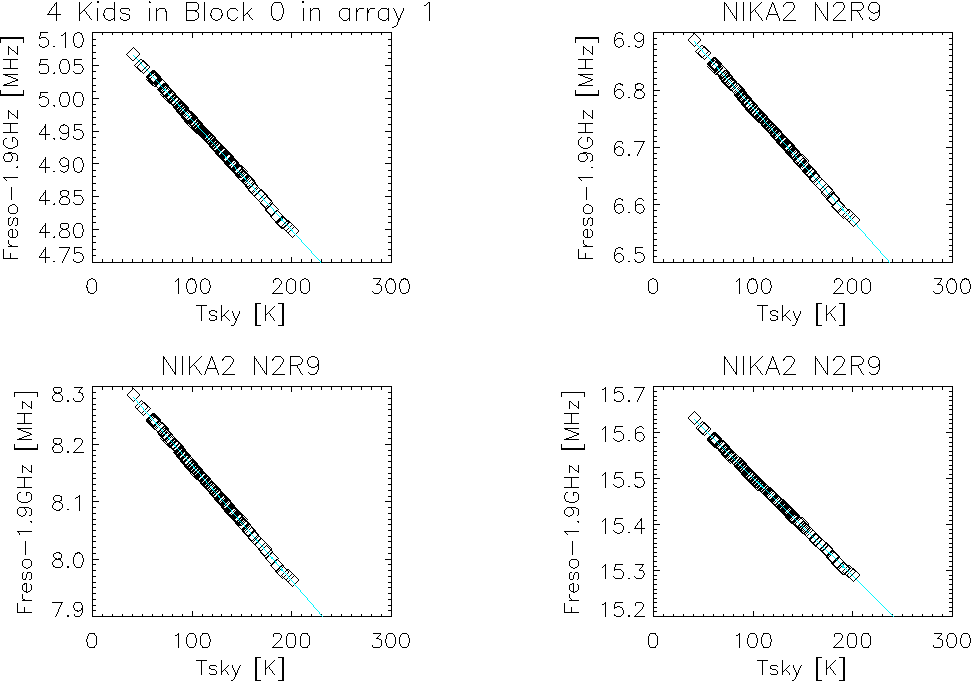
\includegraphics[clip=true,width=0.8\textwidth]{Figures/Opacity/test_allskd4_N2R9v5_5-crop.pdf}
\caption[]{Example of the global skydip fit for four KIDs (one per plot).
Each square point represents one step in a skydip (made of eleven
elevation steps). 12 skydips are used together spanning zenith
opacities from 0.15 to 0.50. The horizontal axis gives the sky
effective temperature $T_{atm}[1-e^{-\tau x}]$ where $\tau$ is the
skydip zenith opacity found in the fit. The vertical axis shows the
resonance frequency of the KID. The blue line is the expected linear
fit implied by the found $c_0^k$ and $c_1^k$ coefficients (see
Eq.~\ref{eq:skydip}). }
\label{fig:skydipfitexample}
\end{center}
\end{figure}

We observe that the skydip-fitted $\tau$ values are, as expected,
common between different detectors of the same array. By comparing the
results of different skydips, we have verified experimentally that the
coefficients $c_0$, $c_1$ are stable, within the fit errors, on very
long time scales within a cooldown cycle. The coefficients can thus be
applied to the whole observing campaign in order to recover the
opacity of each scan. Fig.~\ref{fig:skydip-stability} illustrates the
stability of $c_0$ converted to equivalent temperature of the
background. There is no apparent change of that background by more
than 0.5~K.

%\noindent {\bf FM : a figure would help to convince the reader that it is stable on lng time
% scale, which is a key point.}\\ {\color{magenta} FXD: I will do that figure}

The skydip-based procedure consists in fitting a couple of paramaters
($c_0$, $c_1$) for each of the several thousand valid KIDs. This
requires to have on hands a sizable amount of skydip scans --
typically ten to twenty -- that i) span the whole opacity range and
ii) avoid highly perturbated atmosphere to meet the plane-parallel
atmosphere assumption. To that aim, we recommand to perform a skydip
scan twice a day during a scientific campaign. Then the ($c_0$, $c_1$)
determination process relies on a selection of the skydip scans.




%----------------------------------------------------------------------------------------
%	skydip selection
%----------------------------------------------------------------------------------------
\section{Skydip selection {\color{YellowGreen} Laurence}}
\label{se:skydip-selection}

\begin{figure}[ht!]
\begin{center}
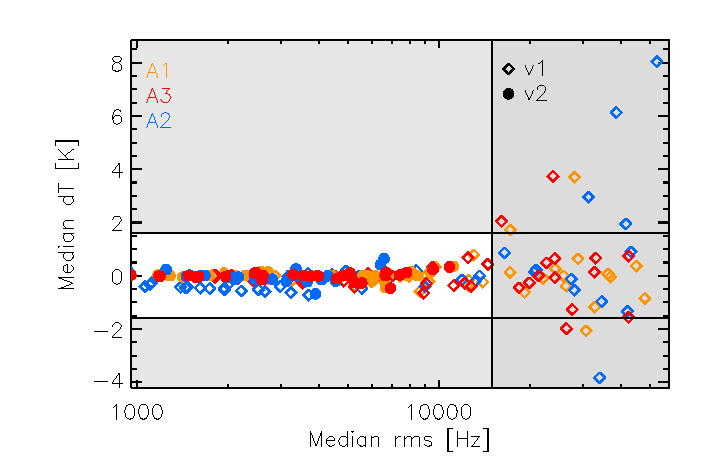
\includegraphics[clip=true,width=0.8\textwidth]{Figures/Opacity/plot_skydip_selection_two_crit.pdf}
\caption[N2R9 skydip scan selection.]{ Median dT quality-fit criterion is plotted in fonction of Median rms criterion for each skydip scans of the N2R9 campaign and for the three arrays. Both criteria are nicely correlated. Empty diamonds show the results of the first iteration of the skydip coefficient estimation, whereas filled circled show the second iteration, for which only the skydips that met both fit-quality criteria are included. After the second iteration, all the remaining skydips met the criteria.}
\label{fig:skydipselection}
\end{center}
\end{figure}

For each skydip scan and for each bunch of 40 KIDs, we compute the
difference between the measured KID resonance frequency and the model
given in Eq.~\ref{eq:skydip} taken at the best-fit values of the
($c_0$, $c_1$) parameters. Then we determine two indicators of the fit
quality per skydip. First, the standard deviation of the
measure-to-model difference is calculated over all the KIDs in a
bunch. For each skydip, we evaluate the median rms, which is the
median over the KID bunches of the standard deviation per bunch, given
in Hz. Secondly, for each scan, we compute the average
measure-to-model difference of each KID $k$, labelled $dT_k$, which is
then converted from Hertz to Kelvin using the $c_1$ parameter of the
KID $k$. Median $dT$ is the median of $dT_k$ over all the KID of an
array. With these two indicators in hands, we discard the skydip scans
that are noisy or that yield a poor fit by applying the selection
criteria

\begin{itemize}
\item Median $\rm{rms} < 1.5 \times 10^{4}~\rm{Hz}$
\item Median $dT < 1.6~\rm{K}$
\end{itemize}

The threshold values have been determined using the set of 44 skydip
scans of N2R9. The Median rms cut corresponds to twice the median of
this quantity per skydip scan, whereas the Median $dT$ cut is twice
the standard deviation of Median $dT$ over the skydips.
N2R9 skydip scan selection is illustrated in
Fig.~\ref{fig:skydipselection}, in
which the agreement between the two fit-quality criteria is clearly
seen. The ($c_0$, $c_1$) estimation proceeds in two steps: first the
parameters are estimated using all the available skydip scan for a
given campaign, then the estimation is re-iterated using the only
skydip scans that met the fit-quality criteria. After the second
iteration, we check that no extra skydip outlier are left, as shown by
the 'v2' label data points in Fig.~\ref{fig:skydipselection}. After
selection of the skydip scans acquired during the N2R9 campaign, 15
skydips are kept for the final step of the ($c_0$, $c_1$) fit. 

\begin{figure}[ht!]
  \begin{center} \includegraphics[clip=true, trim={0, -0.3cm, -0.3cm,
    0},
    width=0.42\textwidth]{Figures/Opacity/test_allskd4_N2R9v3_3-crop.pdf} \includegraphics[clip=true,
    trim={0, -0.3cm, -0.3cm, 0},
    width=0.42\textwidth]{Figures/Opacity/test_allskd4_N2R9v3_4-crop.pdf} \caption[]{(left)
    rms dispersion of the skydip fit to the KIDs resonance frequency
    for almost all N2R9 skydips. The rms gives the quality of the
    plane-parallel hypothesis. (right) evolution of the background as
    observed by NIKA2 during the N2R9 run. During the whole run, there
    is no particular trend of that background with time (except for
    anomalous skydips).  }
\label{fig:skydip-stability}
\end{center}
\end{figure}

\begin{figure}[ht!]
  \begin{center}
    \includegraphics[clip=true, trim={0, -0.3cm, -0.3cm, 0},  width=0.42\textwidth]{Figures/Opacity/Skydip_selection_impact_a1.pdf}
    \includegraphics[clip=true, trim={0, -0.3cm, -0.3cm, 0},  width=0.42\textwidth]{Figures/Opacity/Skydip_selection_impact_a3.pdf}
    \includegraphics[clip=true, trim={0, -0.3cm, -0.3cm, 0},  width=0.42\textwidth]{Figures/Opacity/Skydip_selection_impact_1mm.pdf}
    \includegraphics[clip=true, trim={0, -0.3cm, -0.3cm, 0},  width=0.42\textwidth]{Figures/Opacity/Skydip_selection_impact_a2.pdf}
   \caption[Skydip selection impact on opacities]{Skydip-selection
    impact on the opacity estimates. For a series of calibration scans
    of MWC349 acquired during N2R9, the relative difference
    w.r.t. the baseline opacities $\tau_{\rm{base}}$ (labeled 'base')
    are shown as a function of $\tau_{\rm{base}}$ for five skydip
    selections. The most inclusive one (labeled 'incl')
    includes 38 skydips of the 44 available. 'night' comprizes 11
    skydips acquired during nighttime. 'low' consists of 20 skydips
    acquired in low opacity conditions. 'high
    1' and 'high 2' are fit-quality based selections relying of relaxed
    ('high1') or tighened ('high 2') criteria w.r.t. the baseline
    criteria given in Sect.~\ref{se:skydip-selection}. The dashed
    lines figure a $10\%$ opacity difference
    w.r.t. $\tau_{\rm{base}}$. {\color{blue} FXD: Legend of the figure in percent?}
} 
\label{fig:skydip-selection-impact}
\end{center}
\end{figure}



We test the stability of the ($c_0$, $c_1$) parameters against the
exact choice of the selection criteria.
We derive ($c_0$, $c_1$) parameter sets for the N2R9 campaign using
six skydip selections: the baseline selection (labeled 'base')
consists in the fit-quality based selection described above, which
comprizes 15 skydips, the selection labeled 'incl' consists of an
inclusive selection of 38 skydips in which only the noisier ones were
discarded, the 'night' selection comprizes 11 skydips acquired during
between 21:00 and 09:00 UT,
'high 1' and 'high 2' are two different selections, which comprize 23
and 13 skydips and are based on fit quality criteria that are
respectively relaxed or tighened with respect to the baseline criteria, 
and 'low' corresponds to a selection of 20 skydips acquired while
$\tau_{1mm} < 0.44$. Each ($c_0$, $c_1$) sets are used to derive
zenith opacity of the N2R9 calibration scans of MWC349. 
Figure~\ref{fig:skydip-selection-impact} shows the relative
difference between each $\tau$ estimates and the baseline $\tau$
estimates as a function of the baseline $\tau$. The relative
differences are basically constant for the whole opacity range: the
main effect of the skydip selection is a normalisation factor on the
$\tau$ estimates at both wavelength. At both wavelength, this factor
is below $10\%$ of the baseline $\tau$ for most of the skydip
selections. However, this is of about $10\%$ for the 'low' selection,
which highlight the necessity of including good skydips acquired in
high $(\tau_{1\rm{mm}} > 0.44)$ opacity conditions in the final
selection. The 'incl' (inclusive 38-skydip based) selection results in the larger
difference w.r.t. the baseline $\tau$, which are up to $20\%$ at 1mm
and up to $40\%$ at $2$mm, whereas the 'high 1' (mild quality-fit)
selection suffices to reduce the relative difference below $10\%$ at
1mm and below $15\%$ at 2mm.
As a summary, the $\tau$ estimates are robust against the exact skydip
selection as long as the selection includes good
skydips in high opacity condition $(\tau_{1\rm{mm}} > 0.44)$ and as the poor
fitting skydips are excluded. When these conditions are met, the
skydip selection induced uncertainties are below $10\%$ at 1mm and
below $15\%$ at 2mm. 

We conclude that opacities at both wavelengths can be reliably
estimated from a series of skydip scans using the ($c_0$, $c_1$) model.


%We conclude that opacities at 1mm can be reliably estimated from a series of skydip scans using the (C0, C1) model. %By contrast, for the 2mm opacities, a skydip-based method is not stable enough against the skydip selection. Thus, we adopt an hybrid approach. 

%\section{The hybrid method}

%The hybrid method comprizes two-steps: i) first the 1mm opacities,
%that are $\tau_{A1}$ and $\tau_{A3}$, are determined using the skydip
%method described in Sect.~\ref{se:skydip-method}, ii) then the 2mm
%opacity $\tau_{A2}$ is extrapolated from the 1mm ones using a modified
%ATM model. Namely, for the second step, we perform:

%\begin{equation}
%\tau_{A2} = \left( \left.\frac{\tau_{A2}^{\rm{ATM}}}{\tau_{A3}^{\rm{ATM}}}\right\vert_{\tau_{A3}} + \alpha \right) \tau_{A3},
%\end{equation}

% where $\alpha$ is an offset, which are estimated from the observations themselves, and the ratio is the predicted zenith opacity ratio for A2 and A3 frequency bands using the ATM model described in \ref{Pardo2002} and taken at the measured A3 zenith opacity. The zenith opacity expectations for the array $A_i$ is
%\begin{equation}
%  \tau^{\rm{ATM}}_{A_i} = - \ln{\frac{\int e^{-\tau^{ATM}(\nu)} T_{A_i}(\nu) d\nu}{ \int T_{A_i}(\nu) d\nu}},
%\end{equation}
%where the bandpasses $T_{A_i}$ for arrays $A_i$, $i=1, 2, 3$, are the Martin-Pupplet reference transmissions
%corrected by a Rayleigh-Jeans term  $T'_{A_i}(\nu) / \left( \frac{\nu}{\nu_0}\right)^2$. 

%We observe that the measured \emph{shape} of the measured opacity ratio is well described by the ATM expectations whereas its \emph{amplitude} is too low by an offset $\alpha$, which we dertermine using a data-driven approach. We estimate $\alpha$ as the offset that ensures a stability of the A2 flux over the whole opacity span.  

%\addparag{$\alpha$ fit + FIG}


%----------------------------------------------------------------------------------------
%	skydip opacity tests
%----------------------------------------------------------------------------------------
\section{Skydip-based opacity measurements and tests {\color{YellowGreen} Laurence}}
\label{se:skydip-opacity_tests}

We perform basic sanity tests of the zenith opacity measurements using
the skydip-based method discussed in Sect.~\ref{se:skydip-method}, and
that are referred to as 'skydip' opacities hereafter.

First, we test the stability of the 'skydip' opacities from one
observation campaign to another.
Figure~\ref{fig:skydip-to-taumeter-correl} shows the
correlation between the 'skydip' $\tau$ estimates $\tau_{\rm{skydip}}$
and the IRAM $225$ GHz taumeter zenith opacities $\tau_{225}$, which
are described in Sect.~\ref{se:taumeter-method}, for a series of scans
of Uranus and MWC349 acquired during three campaigns. As guidelines,
we also show the predicted correlations using an ATM model integrated
in NIKA2 wavebands. At 1~mm, the
$\tau_{\rm{skydip}}$ to $\tau_{225}$ correlation relations are
consistent for the three campaigns. They are
also in agreement with the ATM model expectations. At 2~mm, more
dispersion is observed between each correlation relations although
they are compatible with each others within statistical errors.
We note that the ATM model underestimates the
measured $\tau_{\rm{skydip}}$. This mild discrepancy with the
ATM model predictions is yet to be understood, but has no impact on
our opacity measurements, which do not rely on any ATM model nor on
the precision with which the observing bandpasses are known.


\begin{figure}[ht!]
  \begin{center}
    \includegraphics[clip=true, trim={0, -0.3cm, -0.3cm, 0}, width=0.42\textwidth]{Figures/Opacity/Opacity_correl_skydip_vs_tau_a1.pdf}
    \includegraphics[clip=true, trim={0, -0.3cm, -0.3cm, 0}, width=0.42\textwidth]{Figures/Opacity/Opacity_correl_skydip_vs_tau_a3.pdf}
    \includegraphics[clip=true, trim={0, -0.3cm, -0.3cm, 0}, width=0.42\textwidth]{Figures/Opacity/Opacity_correl_skydip_vs_tau_1mm.pdf}
    \includegraphics[clip=true, trim={0, -0.3cm, -0.3cm, 0}, width=0.42\textwidth]{Figures/Opacity/Opacity_correl_skydip_vs_tau_a2.pdf}
   \caption[NIKA2 skydip-based vs taumeter opacities]{ NIKA2
    skydip-based opacities vs IRAM 225GHz taumeter opacities. The
    modeled correlations relying on an ATM model integrated in NIKA2
    bands are shown in black.} 
\label{fig:skydip-to-taumeter-correl}
\end{center}
\end{figure}

We check the robustness of the 'skydip' $\tau$ againts the
observing elevation. 
Figure~\ref{fig:skydip-to-taumeter-ratio-vs-elev} shows the ratio of NIKA2
'skydip' opacities to the $225$ GHz taumeter opacities as a function of
the average scan elevation. The 'skydip' opacity measurements have no
sizable dependency on the elevation. Moreover, the
'skydip'-to-taumeter opacity ratios derived for Uranus scans and for
the scans of the secondary calibrator MWC39 are in good agreement.

\begin{figure}[ht!]
  \begin{center}
    \includegraphics[clip=true, trim={0, -0.3cm, -0.3cm, 0}, width=0.42\textwidth]{Figures/Opacity/Opacity_skydip_to_taumeter_vs_elev_a1.pdf}
    \includegraphics[clip=true, trim={0, -0.3cm, -0.3cm, 0}, width=0.42\textwidth]{Figures/Opacity/Opacity_skydip_to_taumeter_vs_elev_a3.pdf}
    \includegraphics[clip=true, trim={0, -0.3cm, -0.3cm, 0}, width=0.42\textwidth]{Figures/Opacity/Opacity_skydip_to_taumeter_vs_elev_1mm.pdf}
    \includegraphics[clip=true, trim={0, -0.3cm, -0.3cm, 0}, width=0.42\textwidth]{Figures/Opacity/Opacity_skydip_to_taumeter_vs_elev_a2.pdf}
    \caption[NIKA2 skydip-based opacity stability against observing elevations]{NIKA2
    skydip-based opacities stability againts the observing elevation.} 
\label{fig:skydip-to-taumeter-ratio-vs-elev}
\end{center}
\end{figure}

As a summary, the 'skydip' opacity estimates i) have reproducible
correlation coefficients with the 225 GHz taumeter opacities from a
campaign to another, ii) are robust againts the observing conditions,
and iii) are stable for various sources. 



%----------------------------------------------------------------------------------------
%	Corrected skydip method
%----------------------------------------------------------------------------------------
\section{Corrected skydip method {\color{YellowGreen} Laurence}}
\label{se:corrected-skydip}

The consistency checks presented in
Sect.~\ref{se:skydip-opacity_tests} constitute first
robustness tests of the 'skydip' opacities. However, the opacity
estimates are ultimately tested by assessing the
stability of the top-of-the-atmosphere flux densities for a large
range of atmospheric conditions, as will be addressed in
Chapter~\ref{se:photometry}. After opacity correction using the
'skydip' method, the calibration flux density measurements show a
residual dependency on the atmospheric transmission, as discussed in
Sect.~\ref{se:photometry_others}. This motivates the development of a
corrected version of the 'skydip' method, which is described in this
section, that ensures the robustness of the flux densities against
atmospheric conditions.


%%%%%%%%%%%%%%%%%%%%%%%%%%%%%%%%%%%%%%%%%%%%%%%%%%%%%%%%%
% 1-params correction
%%%%%%%%%%%%%%%%%%%%%%%%%%%%%%%%%%%%%%%%%%%%%%%%%%%%%%%%%%
We use the flux stability estimators described in
Sect.~\ref{se:taumeter-method} to fit a correction to the 'skydip'
opacities $\tau_{\rm{skydip}}$ as
\begin{equation}  
  \tau_\nu =  a_\nu^{\rm{skydip}}\tau_{\rm{skydip}}.
  \label{eq:corrected_skydip}
\end{equation}

We find $a_\nu^{\rm{skydip}}$ of
$1.36 \pm 0.04$,
$1.23 \pm 0.02$,
$1.27 \pm 0.03$ and
$1.03 \pm 0.03$ for A1, A3, A1$\&$A3 and A2 respectively.
% a   = 1.3600000       1.0318470       1.2326556       1.2660000
% s_a = 0.038587182     0.028553570     0.019324699     0.026832816


%%%%%%%%%%%%%%%%%%%%%%%%%%%%%%%%%%%%%%%%%%%%%%%%%%%%%%%%%
% 2-params correction
%%%%%%%%%%%%%%%%%%%%%%%%%%%%%%%%%%%%%%%%%%%%%%%%%%%%%%%%%%
\begin{figure}[ht!]
  \begin{center}
    \includegraphics[clip=true, trim={0, -0.3cm, -0.3cm, 0}, width=0.42\textwidth]{Figures/Opacity/fit_nika2_tau_from_skydip_mwc349_a1.pdf}
    \includegraphics[clip=true, trim={0, -0.3cm, -0.3cm, 0}, width=0.42\textwidth]{Figures/Opacity/fit_nika2_tau_from_skydip_mwc349_a3.pdf}
    \includegraphics[clip=true, trim={0, -0.3cm, -0.3cm, 0}, width=0.42\textwidth]{Figures/Opacity/fit_nika2_tau_from_skydip_mwc349_1mm.pdf}
    \includegraphics[clip=true, trim={0, -0.3cm, -0.3cm, 0}, width=0.42\textwidth]{Figures/Opacity/fit_nika2_tau_from_skydip_mwc349_a2.pdf}
    \caption[NIKA2 skydip-based opacity correcting
    relation]{Fit of the skydip-based opacity correcting relation
    parameters.
    The flux-stability estimator contours are shown in the plan
    $a_{\rm{skydip}} \equiv a_\nu^{\rm{skydip}'}$ and
    $b_{\rm{skydip}} \equiv b_\nu^{\rm{skydip}'}$
    for A1, A3, A1$\&$A3 and A2.
    The red contours enclose rms
    errors of the measured-to-median flux density ratio of $5.5$, $7$
    and $10\%$ at 1mm and $2.7$, $3.5$ and $5\%$ at 2mm. The blue
    contours correspond roughthly to the $68\%$, $95\%$ and $99\%$
    confidence levels drawn from the $\chi^2$ estimates.
    The best fit values are shows as green stars. Offset
    $b_\nu^{\rm{skydip}'}$ are compatible with zero within the $68\%$
    CL contours.} 
\label{fig:skydip_fit}
\end{center}
\end{figure}

Moreover, we test for an offset $b_\nu^{\rm{skydip}'}$ in the
correcting relation of the 'skydip' opacities as 
\begin{equation}  
  \tau_\nu =  a_\nu^{\rm{skydip}'}\tau_{\rm{skydip}} + b_\nu^{\rm{skydip}'}.      
\end{equation}
We repeat estimating the parameters of the correcting
relation. Confidence level contours in the parameter plan using the
two stability estimators are skown in Fig.~\ref{fig:skydip_fit}, as
well as the
best-fitting parameter values.
We find the best-fit $a_\nu^{\rm{skydip}'}$ estimates of
$1.36 \pm 0.04$,
$1.25 \pm 0.07$,
$1.28 \pm 0.04$ and
$1.05 \pm 0.05$ for A1, A3, A1$\&$A3 and A2 respectively, which are in
agreement with the best-fit values estimated using the single-parameter
correcting relation, whereas the best-fit values of the offsets
$b_\nu^{\rm{skydip}'}$ are compatible with zero at both wavelengths.
% a   = 1.3600000       1.0467126       1.2476650       1.2792013
% s_a = 0.037853031     0.050552977     0.068354972     0.044088207
% b   = -0.0053333333    -0.014432990    -0.040000000    -0.030731707
% s_b = 0.011925696     0.012184154     0.030641294     0.020823168

We conclude that correcting the skydip-based opacity estimes for a
normalisation as given in Eq.~\ref{eq:corrected_skydip} suffices for
ensuring flux density robustness against atmospheric conditions.
NIKA2 baseline results rely on zenith opacity estimes obtained with
the corrected skydip method for the atmospheric attenuation
correction. Assessment of the photometric capabilities using the data
from three onservation campaigns will be addressed in
Sect.~\ref{se:photometry_baseline}.


  % Xavier&Laurence
%----------------------------------------------------------------------------------------
%	OPACITY MEASURES
%----------------------------------------------------------------------------------------

\section{Opacity monitoring}% {\color{YellowGreen} Juan $\&$ Laurence}}
\label{se:opacity_measures}

%{\bf copy from the 'Instru' paper}

%\begin{figure}[ht]
%\begin{center}
%\includegraphics[scale=0.8]{Figures/test_allskd_N2R10v3commiss2.pdf}
%\caption{Atmospheric opacity as measured from the NIKA2 data 
%at 260 (top) and 150\,GHz (bottom) during N2R10
%commissioning campaign. Each block of 40 KIDs gives an independent estimate of
%the opacity value for each skydip scan (the integer abscissae). The block
%number is the decimal value of the abscissae.
%\label{fig:taumeas_paper}}
%\end{center}
%\end{figure}

%\begin{figure}[ht]
%\begin{center}
%\includegraphics[scale=0.8]{Figures/test_allskd_N2R10v2commiss1.pdf}
%\caption{Atmospheric opacity as measured from the NIKA2 data 
%at 260 and 150\,GHz during N2R10
%commissioning campaign. The error bars are in fact dispersion of the deduced
%opacities between blocks of 40 KIDs.
%\label{fig:taumeas_paper}}
%\end{center}
%\end{figure}


\begin{figure}[ht]
\begin{center}
\includegraphics[scale=1.0]{Figures/opacity_evol_run_9_12_14.pdf}
\caption[Zenith opacity monitoring during N2R9, N2R12 and
  N2R14]{Atmospheric opacity as measured from the IRAM 225\,GHz
  taumeter (yellow green), and from the NIKA2 data at 150 (red) and
  260\,GHz (blue) during N2R9 commissioning campaign (Feb. 2017) and
  N2R12 (Oct. 2017) and N2R14 (Jan. 2018) scientific pools. We
  stress the fact that the IRAM 225\,GHz taumeter data is not used for
  the atmospheric correction and is plotted here for comparison only.
  \label{fig:taumeas}}
\end{center}
\end{figure}


%\begin{figure}[ht]
%\begin{center}
%\includegraphics[width=\linewidth]{Figures/opacity_vs_index_N2R9_N2R10.png}
%\caption[Zenith opacity monitoring during N2R9 and N2R10]{Atmospheric opacity as measured from the IRAM 225\,GHz
%  taumeter (black crosses), and from the NIKA2 data at 150 (red) and 260\,GHz (blue) during 
%  N2R9 and N2R10 commissioning campaigns.  We stress the fact that the IRAM 225\,GHz taumeter data is not used for the %atmospheric correction and is plotted here just for comparison.
%  \label{fig:taumeas}}
%\end{center}
%\end{figure}


In Fig.~\ref{fig:taumeas}  we present the evolution of the NIKA2 in-band
opacities for all the 'OTF' scans (about 1300 scans per runs) of the
N2R9 commissioning campaign (Feb. 2017) and N2R12 (Oct. 2017) and
N2R14 (Jan. 2018) scientific pools. These are compared to the IRAM
tau-meter values. For both opacity estimates, plateaux correspond to
the repeated propagation of the last valid value in case of failure of
the opacity measurement. We observe an agreement on the
global trend between the IRAM tau-meter opacity (225\,GHz) and the
NIKA2 values (see also Fig.~\ref{fig:skydip-to-taumeter-correl} and
Fig.~\ref{fig:skydip-to-taumeter-ratio-vs-elev}).

%These latter show, however, a smaller dispersion (less that one percent)



 % Juan&Laurence


\clearpage
%----------------------------------------------------------------------------------------
%	FOCAL PLANE RECONSTRUCTION
%----------------------------------------------------------------------------------------
\chapter{Focal Plane Reconstruction}% {\color{blue} Nico et al.}}
\label{se:fp_reconstruction}
%----------------------------------------------------------------------------------------
%	FOCAL PLANE RECONSTRUCTION
%----------------------------------------------------------------------------------------
%\subsection{Methodology}
\label{se:fov}

\begin{figure}[ht]
\begin{center}
\includegraphics[clip, angle=0, scale = 0.15]{Figures/FOV_A1.png}
\includegraphics[clip, angle=0, scale = 0.15]{Figures/FOV_A2.png}
\includegraphics[clip, angle=0, scale = 0.15]{Figures/FOV_A3.png}
\caption{Nasmyth offsets of each array, from beammap 20170226s415 on
  3C84 (N2R9).}
\label{fig:fov_ex}
\end{center}
\end{figure}

% moved to the average FOV section
%\begin{table}
%\begin{tabular}{|l|l|l|}
%\hline
%Array & Number of valid kids & Fraction of all kids\\
%\hline
%A1 & 793 & 0.75\\
%A2 & 481 & 0.83\\
%A3 & 872 & 0.83\\
%\hline
%\end{tabular}
%\end{table}

In order to determine the pointing offsets of each KID w.r.t. the reference sky
coordinates as commanded by the telescope tracking system, we perform a
``beammap'', that is to say we map a bright and compact source, most of the time
a planet, with a elevation step small enough to meet Nyquist sampling at the 1mm
beam scale, namely 4.8~arcsec. We observe this planet with a raster scan in
(az,el) coordinates, either with fixed elevation subscans or fixed azimuth
subscans. The former has the advantage of low air mass variation across a
subscan, the latter offers an orthogonal scan direction to the former: the
combination of both gives a more accurage determination of the far side
lobes. The data reduction proceeds in two steps.

\paragraph{Step 1.} We apply a median filter per
KID timeline whose width is 4~FWHM and we project one map per KID in Nasmyth
coordinates. This median filter removes most of atmospheric and low frequency
electronic noise efficiently, albeit a slight ringing and flux loss on the
source. However, at this stage, we are only interested in the location of the
observed planet. To derive the Nasmyth coordinates from the provided (az,el)
coordinates, we build the following quantities at each time $t$

\begin{eqnarray}
dx_t &=& \cos el_t\, daz_t - \sin el_t\, del_t \nonumber \\
dy_t &=& \sin el_t\, daz_t + \cos el_t\, del_t \nonumber
\end{eqnarray}

where $el_t$ is the elevation of the reference pointing direction and $daz$ and
$del$ are the pointing offsets w.r.t to the source in azimuth and elevation as
provided by the tracking system. Note that $daz$ is already corrected by the
$\cos el_t$ factor to have orthonormal coordinates in the tangent plane of the sky
and be immune to the geodesic convergence at the poles. We then fit a 2D
elliptical gaussian on each kid map. The centroid of this gaussian is a first
estimate of the KID offsets, FWHM's, ellipticity and sensitivity. We apply a
first KID selection by removing outliers to the statistics on these
parameters. We also discard manually KIDs that show a cross-talk counter part on
their map. At the end of this first step, we are ready to move to a second
stage.

\paragraph{Step 2.} With the Nasmyth offsets derived in step 1, we are now able to
mask out the planet in each KID timeline. This mask is centered on the planet
location as seen by each kid, it is circular and has a radius of 60~arcsec. We
now build a template timeline (a.k.a. ``common mode'') in two steps. First, we
take the median of all samples of all KIDs that are outside this mask at a given
time $t$. This gives a first estimate of the common mode. Second, we
cross-calibrate each KID on this common mode when the KID is outside the mask
and we coadd all these KID cross-calibrated timelines when they are outside the
mask to have the final common mode. In this sum, each KID TOI is weighted by the
inverse of its variance outside the mask. Once we have this common mode in hand,
we cross-calibrate each TOI on it outside the mask and we subtract it to the
entire KID TOI. When then resume to the projection of each KID TOI in Nasmyth
coordinates like in step 1, and the 2D elliptical gaussian fit on the each kid
map. The centroid coordinates and the FWHM are now the final parameters that can
be derived on the current scan.

This analysis is repeated on all the beam maps, which provides statistics and
precision on each KID parameter, together with estimates on KID performance stability.

{\bf show a screen capture of Katana.}\\

% LP: j'ajoute une phrase pour referencer la Figure \ref{fig:fov}
We present an example of the FOV reconstruction in Fig.~\ref{fig:fov_ex}.

\begin{equation}
FOV diameter = \sqrt{4 N_{tot. kids} * gridstep^2/\pi}
\end{equation}

{\bf give the values of gridstep (pitch) both in mm and arcsec on the sky}\\

The same definition applies to ``Effective FOV'' to avoid extra multiplication
by the fraction of valid pixels

\begin{equation}
F\lambda = gridstep\times D(30m)/\lambda
\end{equation}

%\subsection{Average Focal Plane Reconstruction}
\label{avg_kidpar}

\begin{figure}
\begin{center}
\includegraphics[trim=2cm 14cm 5cm 4cm, clip=true,width=0.6\linewidth]{Figures/A1_fwhm_color_count.pdf}
\includegraphics[trim=2cm 14cm 5cm 4cm, clip=true,width=0.6\linewidth]{Figures/A3_fwhm_color_count.pdf}
\includegraphics[trim=2cm 14cm 5cm 4cm, clip=true,width=0.6\linewidth]{Figures/A2_fwhm_color_count.pdf}
\caption{Average detectors positions for arrays A1, A3, and A2 (from
  green to red as a function of the number of times that a given pixel
  has been considered as valid). The three plots show the detectors
  that have seen the sky and passed the quality criteria for at least
  two beam maps during Run10, 9 and 8: 952, 961, and 553
  %925, 944, and 543
  for A1, A3 and A2, respectively. The inner and outer dash-line circles correspond to a FOV of 5.5$\prime$ and 6.5$\prime$, respectively. Units are arcseconds. The color (from green to red)  shows the number of times that a given pixel has been considered as valid.}
\label{fig:avg_fov_color}
\end{center}
\end{figure}

In order to identify the most stable pixels, we compare the KIDs parameter obtained with several beam maps. 
In the following we will show results as obtained using seven beam maps from Run10, two from Run9 and one from Run8.
For each pixel we compute the average position on the focal plane and the average FWHM, counting the times that it has been considered as valid.

In Fig. \ref{fig:avg_fov_color} we show the average focal plane
reconstruction, from green to red depending on the number of times
that the pixel has been considered as valid. For A1, A3 and A2,
respectively, we have 952, 961, and 553 pixels that have been
considered as valid at least twice (840, 508, 868 valid at least five
times).
% LP: add a sentence to reference Table ``\ref{tab:number_of_kids}"
Using this criterion, we deduce the fraction of valid
detectors over the designed ones, as given in Table~\ref{tab:number_of_kids}. 
As a second step, we also flag pixels that move across the focal plane from a beam map to another (Fig. \ref{fig:jumping_kids} , jumping KIDs) and those who share the same position (twin KIDs). To identify the former we look at the difference of the mean and median position of each KID (the red crosses and black squares in Fig. \ref{fig:mean_vs_median}). For the latter a criteria on the position is applied in order to find the pixels that are closer than the grid step.

\begin{figure}
\begin{center}
\includegraphics[trim=2cm 14cm 5cm 4cm, clip=true,width=0.6\linewidth]{Figures/A1_positions.pdf}
\includegraphics[trim=2cm 14cm 5cm 4cm, clip=true,width=0.6\linewidth]{Figures/A3_positions.pdf}
\includegraphics[trim=2cm 14cm 5cm 4cm, clip=true,width=0.6\linewidth]{Figures/A2_positions.pdf}
\caption{For the 952, 961, and 553 pixels that have passed the quality criteria at least twice for A1, A3 and A2, we show the positions of each pixel, as obtained from each beam map. We can see that some of them are not found at the same position for all the beam maps. Units are arcseconds.}
\label{fig:jumping_kids}
\end{center}
\end{figure}

\begin{figure}
\begin{center}
\includegraphics[trim=2cm 14cm 5cm 4cm, clip=true,width=0.6\linewidth]{Figures/A1_test_positions.pdf}
\includegraphics[trim=2cm 14cm 5cm 4cm, clip=true,width=0.6\linewidth]{Figures/A3_test_positions.pdf}
\includegraphics[trim=2cm 14cm 5cm 4cm, clip=true,width=0.6\linewidth]{Figures/A2_test_positions.pdf}
\caption{For the 952, 961, and 553 pixels that
  have passed the quality criteria at least twice for A1, A3 and A2,
  we show the mean (red crosses) and the median (black squares)
  positions of each pixel, as obtained from each beam map.
  Units are arcseconds. }
\label{fig:mean_vs_median}
\end{center}
\end{figure}


% LP: copy from fov.tex + modif according to Samuel's comment
\begin{table}
  \label{tab:number_of_kids}
  \begin{tabular}{|r|r|r|r|}
    \hline
    Array & Number of designed detectors &  Number of valid detectors & Fraction of all detectors\\
    \hline
    A1 & 1140 & 952 &  0.84\\
    A3 & 1140 & 961 &  0.84\\
    A2 & 616  & 553 &  0.90\\
    \hline
  \end{tabular}
\end{table}

%\subsection{FOV grid distortion}
\label{se:grid_distortion}

{\bf LP edit using Samuel's comments, [TBC]}

We studied the matching of the KIDs position on the sky to the
\emph{design} position, as decribed in Xavier's wiki post\footnote{see
  {\tt http$://$www.iram.fr$/$wiki$/$nika2$/$index.php$/$}
  
  {\tt April$\_$19,$\_$2017,$\_$FXD,$\_$KID$\_$position$\_$mapping$\_$and$\_$Field$\_$distortion$\_$for$\_$Run9}
}

This has been compared to expectations obtained using ZEMAX
simulation. The grid diagram generated using ZEMAX provides us with
the maximum dispersion in the field defined by

\begin{equation}
P = \frac{\sqrt{(x_p - x_r)^2 + (y_p - y_r)^2}}{\sqrt{x_p^2 + y_p^2}},
\end{equation}

where $(x_p, y_p)$ and $(x_r, y_r)$ are respectivelly the predicted
and real coordinates on the image surface relative to the reference
field position image location (see page 170 of the ZEMAX manual, 2007).
The predicted coordinates for the whole field are obtained using a
linear interpolation of a small area in the field central part,
whereas the real coordinates are calculated by ray tracing through the
optical system.

\begin{figure}[ht] 
\begin{center}
\includegraphics[width=0.9\textwidth]{Figures/NIKA2_Final_grid.png}
\caption{NIKA2 grid diagram simulated using ZEMAX. Crosses indicate
  the real coordinates on the Nasmyth image plan. {\bf question a
    Samuel: pourquoi les dimensions indiquees sont environs 4.5 arcmin
  de cote (et pas 6.5)?}}
 \label{fig:fov_grid_distortion_zemax}
\end{center}
\end{figure}

Figure \ref{fig:fov_grid_distortion_zemax} show the ZEMAX grid diagram for
NIKA2 simulated optic system. The maximum grid distortion is expected
to be of $2.7\%$ in NIKA2 $6.5'$ FOV. The distortion is the most
noticeable in the upper right corner of the Nasmyth plan, which is
also the area of the largest defocus w.r.t. to the center. 




%   Geometry
%----------------------------------------------------------------------------------------
\subsection{Focal Plane Geometry}

In order to determine the pointing offsets of each KID with respect to the reference sky
coordinates as commanded by the telescope tracking system, we use beam-maps. 
The data reduction proceeds in two steps.

\paragraph{Step 1.} We apply a median filter per
KID timeline whose width is 4~FWHM and we project one map per KID in Nasmyth
coordinates. This median filter removes efficiently most of the atmospheric and low frequency
electronic noise, albeit a slight ringing and flux loss on the
source. However, at this stage, we are only interested in the location of the
observed planet. To derive the Nasmyth coordinates from the provided (az,el)
coordinates, we build the following quantities at time~$t$ :

\begin{eqnarray}
dx_t &=& \cos el_t\, daz_t - \sin el_t\, del_t \nonumber \\
dy_t &=& \sin el_t\, daz_t + \cos el_t\, del_t \nonumber
\end{eqnarray}

\noindent {\bf FM: why not using $\delta$ as in the previous section ?}\\
\noindent {\bf FM: i don't think the $_t$ is useful}\\


where $el_t$ is the elevation of the reference pointing direction and $daz$ and
$del$ are the pointing offsets with respect to the source in azimuth and elevation as
provided by the tracking system. Note that $daz$ is already corrected by the
$\cos el_t$ factor to have orthonormal coordinates in the tangent plane of the sky
and be immune to the geodesic convergence at the poles. We then fit a 2D
elliptical gaussian on each kid map. The centroid of this gaussian is a first
estimate of the KID offsets, FWHM's, ellipticity and sensitivity. We apply a
first KID selection by removing outliers to the statistics on these
parameters. We also discard manually KIDs that show a cross-talk counter part on
their map. 
%At the end of this first step, we are ready to move to a second stage.

\paragraph{Step 2.} With the Nasmyth offsets derived in step 1, we are now able to
mask out the planet in each KID timeline. This mask is centered on the planet
location as seen by each kid, it is circular and has a radius of 60~arcsec. We
now build a template timeline (a.k.a. ``common mode'') in two steps. First, we
take the median of all samples of all KIDs that are outside this mask at a given
time $t$. This gives a first estimate of the common mode. Second, we
cross-calibrate each KID on this common mode when the KID is outside the mask
and we coadd all these KID cross-calibrated timelines when they are outside the
mask to have the final common mode. In this sum, each KID TOI is weighted by the
inverse of its variance outside the mask. Once we have this common mode in hand,
we cross-calibrate each TOI on it outside the mask and we subtract it to the
entire KID TOI. We then resume to the projection of each KID TOI in Nasmyth
coordinates like in step 1, and the 2D elliptical gaussian fit on the each kid
map. The centroid coordinates and the FWHM are now the final parameters that can
be derived on the current scan.

This analysis is repeated on all beam maps, which provides statistics and
precision on each KID parameter, together with estimates on KID performance stability.



{\bf FM : {\it precision} ? }\\
{\bf show a screen capture of Katana.}\\

% LP: j'ajoute une phrase pour referencer la Figure \ref{fig:fov}
We present an example of the FOV reconstruction in Fig.~\ref{fig:fov_ex}.

The FOV diameter is defined as 
\begin{equation}
FOV diameter = \sqrt{4 N_{tot. kids} \times gridstep^2/\pi}
\end{equation}

{\bf give the values of gridstep (pitch) both in mm and arcsec on the sky}\\

The same definition applies to ``Effective FOV'' to avoid extra multiplication
by the fraction of valid pixels

\begin{equation}
F\lambda = gridstep\times D(30m)/\lambda
\end{equation}




%   KID selection
%----------------------------------------------------------------------------------------
\subsection{KID selection and average geometry}
\label{avg_kidpar}


\begin{figure}[p]
\begin{center}
\includegraphics[trim=2cm 14cm 4cm 4cm, clip=true,width=0.55\linewidth]{Figures/A1_fwhm_color_count.pdf}
\includegraphics[trim=2cm 14cm 4cm 4cm, clip=true,width=0.55\linewidth]{Figures/A3_fwhm_color_count.pdf}
\includegraphics[trim=2cm 14cm 4cm 4cm, clip=true,width=0.55\linewidth]{Figures/A2_fwhm_color_count.pdf}
\caption{Average detectors positions for arrays A1, A3, and A2 (from
  green to red as a function of the number of times that a given pixel
  has been considered as valid). The three plots show the detectors
  that have seen the sky and passed the quality criteria for at least
  two beam maps during Run10, 9 and 8: 952, 961, and 553
  %925, 944, and 543
  for A1, A3 and A2, respectively. The inner and outer dash-line circles correspond to a 
  FOV of 5.5$\prime$ and 6.5$\prime$, respectively. Units are arcseconds. 
  The color (from green to red)  shows the number of times that a given pixel has been considered as valid.}
\label{fig:avg_fov_color}
\end{center}
\end{figure}

In order to identify the most stable pixels, we compare the KIDs parameter obtained with several beam maps. 
In the following, we   show results as obtained using seven beam maps from Run10, two from Run9 and one from Run8.
For each pixel we compute the average position on the focal plane and the average FWHM, counting the times that it has been considered as valid.

In Fig. \ref{fig:avg_fov_color} we show the average focal plane
reconstruction, from green to red depending on the number of times
that the pixel has been considered as valid. For A1, A3 and A2,
respectively, we have 952, 961, and 553 pixels that have been
considered as valid at least twice (840, 508, 868 valid at least five
times).
% LP: add a sentence to reference Table ``\ref{tab:number_of_kids}"
Using this criterion, we deduce the fraction of valid
detectors over the designed ones, as given in Table~\ref{tab:number_of_kids}. 
As a second step, we also flag pixels that move across the focal plane from a 
beam map to another (Fig. \ref{fig:jumping_kids} , jumping KIDs) and those 
who share the same position (twin KIDs). To identify the former, we look at the difference 
of the mean and median position of each KID (the red crosses and black squares in 
Fig. \ref{fig:mean_vs_median}). For the latter a criterion on the position is applied in 
order to find the pixels that are closer than the grid step.



\noindent {\bf FM: how many twins ? how many jumping kids ?}\\


\begin{figure}[htp]
\begin{center}
\includegraphics[trim=2cm 14cm 5cm 4cm, clip=true,width=0.55\linewidth]{Figures/A1_positions.pdf}
\includegraphics[trim=2cm 14cm 5cm 4cm, clip=true,width=0.55\linewidth]{Figures/A3_positions.pdf}
\includegraphics[trim=2cm 14cm 5cm 4cm, clip=true,width=0.55\linewidth]{Figures/A2_positions.pdf}
\caption{For the valid detectors, we show the positions of each pixel, as obtained from 
each beam map. Some of them are not found at the 
same position for all the beam maps. Units are arcseconds. {\bf FM : color code ?}}
\label{fig:jumping_kids}
\end{center}
\end{figure}

\begin{figure}[htp]
\begin{center}
\includegraphics[trim=2cm 14cm 5cm 4cm, clip=true,width=0.55\linewidth]{Figures/A1_test_positions.pdf}
\includegraphics[trim=2cm 14cm 5cm 4cm, clip=true,width=0.55\linewidth]{Figures/A3_test_positions.pdf}
\includegraphics[trim=2cm 14cm 5cm 4cm, clip=true,width=0.55\linewidth]{Figures/A2_test_positions.pdf}
\caption{For the valid detectors,
  we show the mean (red crosses) and the median (black squares)
  positions of each pixel, as obtained from each beam map.
  Units are arcseconds. {\bf FM : color code ?}}
\label{fig:mean_vs_median}
\end{center}
\end{figure}


% LP: copy from fov.tex + modif according to Samuel's comment
\begin{table}[ht]
\begin{center}  
  \begin{tabular}{|c|c|c|c|}
    \hline
    Array & Designed detectors &  Valid detectors & Fraction\\
    \hline\hline
    A1 & 1140 & 952 &  84\%\\
    A3 & 1140 & 961 &  84\%\\
    A2 & 616  & 553 &  90\%\\
    \hline
  \end{tabular}
  \caption{ CAPTION}
  \label{tab:number_of_kids}
\end{center}    
\end{table}




%   Distortion from the grid
%----------------------------------------------------------------------------------------
\subsection{FOV grid distortion}
\label{se:grid_distortion}

We studied the matching of the KIDs position on the sky to the
\emph{design} position, as decribed in detail in this wiki post\footnote{see
  {\tt http$://$www.iram.fr$/$wiki$/$nika2$/$index.php$/$}
  
  {\tt April$\_$19,$\_$2017,$\_$FXD,$\_$KID$\_$position$\_$mapping$\_$and$\_$Field$\_$distortion$\_$for$\_$Run9}
}
The global result is scaling, rotation, and shift parameters for each
array. They are described in Table~\ref{ta:gridmatch}.

\begin{table}[ht]
\label{ta:gridmatch}
\begin{center}
\begin{tabular}{|c|c|c|c|}
\hline
Array 1  &	Array 3   &	Array 2   &	Comment \\
\hline
1 mm      &       1 mm     &        2 mm  & \\
1140 	 &      1140 	   &        616  &	Total of designed Kids \\
736/673  &	758/734  &	444/437  &	Found/Well-placed Kids \\
91/59 	 &    96/64 	 &      98/71 	 & Fraction [\%] of WPK/FoundKids and WPK/Total \\
0.87 	 &     0.84 	  & 0.66     &	Median deviation (arcsec) for pixels with a deviation smaller than 5 arcsec. \\
0.52 	 &     0.69 	 &        0.68 	 & Mean distortion across the FoV in arcsec \\
2.3 -4.5  &	2.0 -5.8  &	9.3 -7.5  &	Array center in Nasmyth coordinates (arcsec) \\
4.90  &	4.88  &	4.88  &	Plate scaling (arcsec/mm) in the Design x and y (averaged) \\
77.3  &	76.4  &	78.2  &	Plate rotation angle (degree) from the Design to Nasmyth coordinates \\
6.6  &	6.6  &	6.6  &	FOV (Total kids) \\
9.8/2.00  &	9.7/2.00  &	13.3/2.75  &	Distance between near detectors [arcsec, mm] \\
1.24  &	1.22  &	0.97  &	Distance between near detectors [in lambda/D] \\
\end{tabular}
\end{center}
\caption{Linear 2D fit of the observed position of the detectors in the sky
  against their mechanical designed position for N2R9. }
\end{table}

It shows that on average the position of each detector is known to better than
an arcsecond. The 1mm arrays have almost the same center but this center
differs by 7 and 2 arseconds from the 2mm array center. The sampling is above
$\lambda/D$ at 1 mm. Note that the plate rotation angle was designed as
76.2\,degrees, less than 2 degrees from what is observed. We find that array 1
has the most deviant detectors (above 4 arcseconds from their expected
position). These detectors should be excluded from further analysis. We call
distortion (in the table) the $x.y$ term in the polynomial fitting between the
design grid and the observed position (the fitting is done with the $x$ and
$y$ linear terms and $x.y$ term). 



This has been compared to expectations obtained using ZEMAX
simulation. The grid diagram generated using ZEMAX provides us with
the maximum dispersion in the field defined by

\begin{equation}
P = \frac{\sqrt{(x_p - x_r)^2 + (y_p - y_r)^2}}{\sqrt{x_p^2 + y_p^2}},
\end{equation}

where $(x_p, y_p)$ and $(x_r, y_r)$ are respectivelly the predicted
and real coordinates on the image surface relative to the reference
field position image location (see page 170 of the ZEMAX manual, 2007).
The predicted coordinates for the whole field are obtained using a
linear interpolation of a small area in the field central part,
whereas the real coordinates are calculated by ray tracing through the
optical system.

\begin{figure}[ht] 
\begin{center}
\includegraphics[width=0.9\textwidth]{Figures/NIKA2_Final_grid.png}
\caption{NIKA2 grid diagram simulated using ZEMAX. Crosses indicate
  the real coordinates on the Nasmyth image plan. {\bf question a
    Samuel: pourquoi les dimensions indiquees sont environs 4.5 arcmin
  de cote (et pas 6.5)?}}
 \label{fig:fov_grid_distortion_zemax}
\end{center}
\end{figure}

Figure \ref{fig:fov_grid_distortion_zemax} show the ZEMAX grid diagram for
NIKA2 simulated optic system. The maximum grid distortion is expected
to be of $2.7\%$ in NIKA2 $6.5'$ FOV. The distortion is the most
noticeable in the upper right corner of the Nasmyth plan, which is
also the area of the largest defocus w.r.t. to the center. 

An expected distortion of $2.7\%$ is at most a 5 arcsecond shift from the
center to the outside of the array.  The quoted measured distortions are not
too dissimilar once the different fitting methods have been taken into
account.

% FXD: this would need to be more ascertained. Lack of time to go further.


%% [Optimal Focus]
%%________________________________________________________
\subsection{Reconstruction of the focus surfaces}
\label{sec:focus}

Owing to the NIKA2 $6.5~\rm{arcmin}$ FOV, the focus is expected to
slightly changes across the FOV, defining curved focal surfaces at the
location of the three arrays. Therefore, beam patterns are expected to
show some scatter across the FOV accordingly to the focal
surfaces. Although all the detectors cannot be individually focalised,
an optimal axial focus of the telescope can be found to maximize the
number of detectors at the best focus and hence, maximize the
resolution of the NIKA2 maps.
This optimal z-focus setting is obtained
in measuring the focus at the center of the arrays as described
Sect.~\ref{sec:focus-meas} and apply a focus shift, which is primary
predicted using Zemax simulation, and ultimately verified by measuring
the focus surfaces as decribed here.

\begin{figure}
\begin{center}
  \includegraphics[trim={0, 1cm, 0, 1cm}, clip, angle=0, scale=0.5]{Figures/fov_focus_mv_5.png}
\caption{Focus surface of A1, A3 and A2 arrays from left to
  right. From top to bottom, the focus estimates rely on
  FWHM-minimization, amplitude-maximization of an elliptical
  Gaussian of fixed FWHMs and amplitude-maximization of an elliptical
  Gaussian.}
\label{fig:focus-surfaces}
\end{center}
\end{figure}

\emph{Method. } We measure NIKA2 focal surfaces by means of a sequence of five 'beam-map'
scan observations of bright point-like sources, typically Planets or
bright quasars,
for various settings of the telescope axial focus around the
optimal focus $z_{\rm{opt}}$. A beam-map scan consists of a deep-integrated
$13.5' \times 7.8'$ OTF-scan observation comprizing $99$ sub-scans and
with a scanning speed of either $65''/s$ whenever the mean integration
elevation is $< 60$ degree or $39"/s$ at higher elevation. The z-focus is changed in step of
$0.6~\rm{mm}$ to probe a large focus range for measuring even the
extreme variation of the focus surfaces,
namely $z \in \{-1.2, -0.6, 0, 0.6, 1.2 \} + z_{\rm{opt}}$.
Each beam-map scans allow for $4''$-resolution individual maps per kid to
be projected. Before the projection, the correlated noise is mitigated
from each KID timeline in subtrating out a common mode, which is obtained
using, amongst the other detectors, those that correlates the most
with this KID and that are located outside a radius of $90''$
around the source centroid.
Therefore, a series of five cleaned maps at various focus is
available for each detector, from which the best focus is estimated as
described in Sect.~\ref{sec:focus-meas}. The ensemble of the relative
focus estimate per KIDs with respect to the best focus at the center
of the array constitutes the focus surface. An accurate estimate of
the center focus is obtained as the
weighted average focus estimate of the KIDs lying in a $30''$ radius
around the geometrical center of the array. This average does not
induce any sizeable bias thanks to the flatness of the focus surface
in the innermost regions. For robustness test, we consider three focus
estimates: the two first ones are the same as discussed in
Sect.~\ref{sec:focus-meas} -- namely i) $\hat z_{\rm{fwhm}}$ the focus that
minimizes the geometrical FWHM and ii) $\hat z_{\rm{peak}}$ the focus
that maximizes the amplitude of the best-fitting ellitical Gaussian --
whereas the third one is $\hat z_{\rm{flux}}$ the focus that maximizes
the amplitude of the best-fitting elliptical Gaussian of fixed FWHM
(at $12''$ at $260~\rm{GHz}$ and $18''$ at $150~\rm{GHz}$). The 
comparison between the two amplitude-based estimators
($\hat z_{\rm{peak}}$ and $\hat z_{\rm{flux}}$), will test the
stability of the focus results against the exact choice of the beam fitting
function. Since the ellipticity-based estimator $\hat z_{\rm{ellip}}$ is
less sensitive to focus changes and yields larger uncertainties than the
others, we do not use it for the focus surface reconstruction.     


\emph{Data selection. }
During the three commissioning campaigns that occured after the change of A1
lens and the improvement of internal optics alignment (hence in the
final NIKA2 optic configuration),
nine out-of-focus
beam-map scan sequences have been acquired, including incomplete
sequences and sequences hindered by poor atmospheric conditions. We
select sequences that i) comprises at least four scans, ii) have been
observed at zenith opacity at $225~\rm{GHz}$ (as indicated by
the IRAM taumeter) below 0.5 and iii) have a maximal central focus
drift between the starting time and the end of the sequence of
$0.5~\rm{mm}$. These criteria preserve five sequences from which focus
surfaces can be reconstructed. Namely, we consider the sequences
$20170226s415\mbox{--}419$, $20170419s133\mbox{--}137$, $20170420s113\mbox{--}117$,
$20170421s160\mbox{--}164$ and $20170424s123\mbox{--}127$, which consist of observations
of the bright quasar '3C84' and Neptune.

\emph{Results. }
For each detector $k$ and each beam-map sequence $s$, we obtain for
the array $a$, a focus measurement $z_k^{a, s} \pm \sigma_k^{a, s}$,
where $\sigma_k^{a, s}$ is the $1\mbox{--}\sigma$ error of the least-square
polynomial fit. The focus surface measurements per array obtained from the five
beam-map sequences are combined using an inverse-variance weighting
scheme to obtain the focus surface estimates 
\begin{equation}
\label{eq:mv_focus_surf}
z_k^{(a)} = \left( \sigma_k^{(a)} \right)^2 \,  \sum_s \frac{z_k^{a,s}}{\left(\sigma_k^{a,s}\right)^2}\, \,  ,
\end{equation}
with uncertainties 
\begin{equation}
\label{eq:error_mv_focus_surf}
\sigma_k^{(a)} = \left[ \sum_s \frac{1}{\left(\sigma_k^{a,s}\right)^2}\right]^{-1/2}\, .
\end{equation}


We present NIKA2 focus surfaces per arrays obtained as in
Eq.~\ref{eq:mv_focus_surf} 
%from the inverse-variance weighted combination of the five
%reconstructed focus surfaces per arrays
in Fig.~\ref{fig:focus-surfaces}.
The three flavours of focus-estimators provide us with focus surfaces
per arrays that are in good agreement with each others and that have a
non-axisymetrical flatten bowl shape consistent with expectations from
simulation {\bf [TBA, as discussed further below]}.
The median defocus (that is the relative focus w.r.t. the center)
across the detectors is about
$-0.1~\rm{mm}$ for the three arrays. Maximal defocus values of about
$-0.6~\rm{mm}$ are found for detectors located in the outer top and
left regions of the FOV. Finally, a fraction comprised between $20$
and $30\%$ of the KIDs has a relative $z\le -0.2~\rm{mm}$.  

We primarily estimate the uncertainty of the focus
surface measurements using the standard deviation between the three
estimators $z_k^{(a)}|_{\rm{fwhm}}$, $z_k^{(a)}|_{\rm{peak}}$ and
$z_k^{(a)}|_{\rm{flux}}$. We found approximatively homogeneous
standard deviation surfaces per arrays, which have median values across
the FOV of about $0.03~\rm{mm}$.
However, we cross-check this error estimate by forming the quadratic mean of
the three inverse-variance error surfaces per arrays, which are defined in
Eq.~\ref{eq:error_mv_focus_surf} and quoted
$\sigma_k^{(a)}|_{\rm{fwhm}}$, $\sigma_k^{(a)}|_{\rm{peak}}$ and
$\sigma_k^{(a)}|_{\rm{flux}}$. This provides us with more optimistic
error surfaces per array, which do not show any clear pattern across
the FOV and which have a median value across the detectors of about
$0.015~\rm{mm}$.  

%[EXPAND THE DISCUSSION ON COMPARISON WITH SIMULATION]

\emph{Stability across sequences. }
By comparing the focus surface obtained from the five individual focus
sequences, we test the stability of the NIKA2 focus surfaces across
the time and the atmospheric conditions. In
Figs.~\ref{fig:focus-stability-H}-\ref{fig:focus-stability-V}, we compare
the defocus along two perpendicular diameters across the
FOV. Although any direction would have been equivalent for this test, we choose to
position the diameters along-with and perpendicular-to the KID geometrical
grid to avoid the scatter due to KID non-alignement in any other
direction. The scatter is further mitigated by considering
four-detector-wide diameters as shown in upper the left corner of
Figs.~\ref{fig:focus-stability-H}-\ref{fig:focus-stability-V}.

{\bf add a sentence to conclude on the stability}


\begin{figure}
  %\begin{center}
  \includegraphics[trim={-2cm, 2cm, 0, 2cm}, clip, angle=0, scale=0.1]{Figures/fov_focus_stability_check_D1.png}
  \begin{center}
  \includegraphics[trim={0, 2cm, 0, 2cm}, clip, angle=0, scale=0.45]{Figures/fov_focus_1D_Vband_5.png}
  \end{center}
  \caption{Stability of the focus surface across the sequences. This
    series of plot show the relative focus with respect to the center
    (defocus) along the 'vertical diameter', that is a band of
    four-detector width across the FOV, which is vertical with respect to
    the detector geometrical grid, as illustrated by the plot in the
    upper left corner. The datapoints show the defocus along the
    'vertical diameter' estimated from the five focus sequences,
    namely $20170226s415\mbox{--}419$ (sky blue),
    $20170419s133\mbox{--}137$ (dark blue), $20170420s113\mbox{--}117$ (red),
    $20170421s160\mbox{--}164$ (yellow) and $20170424s123\mbox{--}127$
    (green), using the $z^{(a)}|_{\rm{fwhm}}$, $z^{(a)}|_{\rm{flux}}$ and
    $z^{(a)}|_{\rm{peak}}$ estimators from top to bottom, and for A1, A3 and
    A2 arrays from left to right. The black datapoints are the five-sequence combined defocus, as
    presented in Fig.~\ref{fig:focus-surfaces}, taken along the
    'vertical diameter', and the errorbars, the
    five-sequence combined defocus errors along the 'vertical
    diameter'.}
\label{fig:focus-stability-H}
\end{figure}


\begin{figure}  
  \begin{center}
  \includegraphics[trim={0, 2cm, 0, 2cm},clip, angle=0, scale=0.45]{Figures/fov_focus_1D_Hband_5.png}
  \caption{Stability of the focus surface across the sequences. Same
    legend as in Fig.~\ref{fig:focus-stability-H}, but for the
    detectors located in an 'horizontal diameter', i.e. a band of
    four-detector width across the FOV, which is horizontal with respect to
    the detector geometrical grid, as illustrated by the plot in the
    upper left corner. }
\label{fig:focus-stability-V}
\end{center}
\end{figure}



% + Focal Plane Geometry
% + KID selection and average geometry
% + FOV grid distortion
% + Reconstruction of the focus surfaces


\clearpage
%----------------------------------------------------------------------------------------
%	BEAM PATTERN
%----------------------------------------------------------------------------------------
\chapter{Beam pattern}% {\color{blue} Laurence et al.} }
\label{se:beams}
% Full Beam Pattern + beam variations
%%
%%
%%      SECTION: BEAM PATTERN 
%%

%% [intro]
%%________________________________________________________

The NIKA2 beam pattern mainly depends on the IRAM 30m telescope and
NIKA2 full (external and internal) optical system characteristics,
whereas the detectors themselve might have an impact at sub-dominant
level (through e.g. time constants or correlated noises).

In this section, we characterize both the main beam, which is
modeled as an elliptical Gaussian, and the full beam pattern including
error beams up to angular scales of 10 arcmin.

%% [Afternoon beam broadening ]
%%________________________________________________________
\section{Telescope-driven beam variations {\color{blue} Laurence}}
\label{se:obsdate_variations}

In this section, we evidence a beam size broadening depending on the
scan observation date. This effect, which mainly impacts late
afternoon observations and is reproducible from a campaign to another,
is probably due to deformations of the main dish subject to the Sun
heating. This is a well-known effect, which also impacts EMIR and was
observed for the previous generation of instrument MAMBO. However,
compared to the period when MAMBO or NIKA were on activity, these
daily deformations have probably strengthen due to the aging of the
main dish white coating.

\subsection{Beam monitoring using bright source scans}

We monitor the time-dependent beam-size variations using all the
available bright source scans acquired at the optimal focus for each
campaign. Bright sources are selected as flux density
estimates above $1\,\rm{Jy}$ at both wavelengths.
The beam size is estimated by fitting a 2D Gaussian from the map and
taking the geometrical FWHM, defined as 
$\rm{FWHM}_{\rm{geom}} = (\rm{FWHM}_x \rm{FWHM}_y)^{1/2}$, where
$\rm{FWHM}_x$ and $\rm{FWHM}_y$ are the best-fitting values of FWHM
along the minor and major axis of the elliptical 2D Gaussian.

% see def of RESULT_FWHM in nk_grid2info.pro line 320
% + see def of params in nika_gauss2d.pro

For Uranus, the FWHM estimates are corrected for the beam broadening due
to the extension of the apparent disc. At the IRAM 30m latitude,
Uranus disc diameter varies from $3.3''$ to $3.7''$. This induces a
broadening of the Gaussian main beam of $0.19 \pm 0.03\,\rm{arcsec}$ at
1-mm and $0.12 \pm 0.02\,\rm{arcsec}$ at 2-mm. Uranus FWMH estimates are
corrected for the average beam widening values. 

\begin{figure}[ht!]
  \begin{center}
    \includegraphics[clip=true, trim={0.9cm, 0.5cm, 0.5cm, 0.5cm}, width=0.4725\textwidth]{Figures/Beams/Beam_monitoring_with_otfs_vs_ut_1mm.pdf}
    \includegraphics[clip=true, trim={0.5cm, 0.5cm, 0.5cm, 0.5cm}, width=0.4875\textwidth]{Figures/Beams/Beam_monitoring_with_otfs_vs_ut_a2.pdf}
    \caption[Beam size monitoring using OTF scans]{Beam size monitoring using OTF scans} 
\label{fig:beam_monitoring_otf}
\end{center}
\end{figure}

\subsection{Beam monitoring using pointing}


\begin{figure}[ht!]
  \begin{center}
    \includegraphics[clip=true, trim={0.9cm, 0.5cm, 0.5cm, 0.5cm}, width=0.4725\textwidth]{Figures/Beams/Beam_monitoring_with_pointings_vs_ut_1mm.pdf}
    \includegraphics[clip=true, trim={0.5cm, 0.5cm, 0.5cm, 0.5cm}, width=0.4875\textwidth]{Figures/Beams/Beam_monitoring_with_pointings_vs_ut_a2.pdf}
    \caption[Beam size monitoring using pointing scans]{Beam size monitoring using pointing scans} 
\label{fig:beam_monitoring_pointing}
\end{center}
\end{figure}

\begin{figure}[ht!]
  \begin{center}
    \includegraphics[clip=true, trim={0.9cm, 0.5cm, 0.5cm, 0.5cm}, width=0.4725\textwidth]{Figures/Beams/Beam_monitoring_with_otfs_vs_ut_compare_pointings_1mm.pdf}
    \includegraphics[clip=true, trim={0.5cm, 0.5cm, 0.5cm, 0.5cm}, width=0.4875\textwidth]{Figures/Beams/Beam_monitoring_with_otfs_vs_ut_compare_pointings_a2.pdf}
    \caption[Beam size monitoring comparison]{Beam size monitoring comparison} 
\label{fig:beam_monitoring_compare}
\end{center}
\end{figure}

%% [Full beam pattern]
%%________________________________________________________
\section{Full beam pattern {\color{blue} Laurence}}
\label{se:fullbeam}

\subsection{Data sets}
\label{se:beammap_set}

The characterization of the IRAM 30-m beam pattern observed through NIKA2 detectors is mainly based on observations of strong compact sources, such as planets including Uranus, Neptune and Mars, and bright quasars. We generally use beam-map scans, which we recall, are deep-integration raster-scan observations that consist of 99 sub-scans placed at intervals of $4.8''$ to cover a total of $13.5' \times 7.8'$. Most of our beam-related analysis are beased on the same set of beam-map scans as previously selected to perform the average FOV reconstruction. The set comprises nine beam-map scans that distribute as one from N2R8, '20170125s243', two from N2R9, '20170224s177' and '20170226s415' and six from N2R10, which are '20170226s425', '20170227s84', '20170419s133', '20170420s113', '20170424s116', '20170424s123'. 


\subsection{Deep beam maps}
\label{se:beammaps}
We present the two-dimensional distribution of the beam in Fig.~\ref{fig:beam}. We primary use a map obtained from a combination of deep observations of strong point sources collected during \emph{NIKA2-run8} and \emph{run9}. Namely, we use 'beammap' OTF scans of Uranus (scan id '20170125s223' and '20170125s243'),  Neptune ('20170224s177') and the bright quasar 3C84 ('20170226s415'). However, we checked the stability of our results on single scan maps, combinations of scans for a single source, and combinations of shallower scans but spanning a large range of scanning direction. The data processing includes a mitigation of the correlated noise, which mainly originates from the atmosphere.  We primarly use a subtraction of a common mode estimated from the most correlated detectors (the so-called 'cm one block' method). However, other methods are tested for assessing the immunity of our results to noise residuals.

\begin{figure}
\begin{center}
  \includegraphics[clip, angle=0, scale=0.4]{Figures/Lobe_map_Combo_v2_dB.pdf}
 \caption[Beam pattern.]{From upper left to lower right, beam maps of array 1 (labeled 'A1'), array 3 ('A3'), the combination of the 1.15mm arrays ('A1$\&$3') and the 2mm array ('A2') are shown in decibel. These maps, which consist of normalized combination of four long OTF scans of bright point sources, are in celestial coordinates and cover a sky area which extend over 10 arcmin.}
\label{fig:beam}
\end{center}
\end{figure}


The deep NIKA2 beam maps reveal some noticeable features, which are
shown in Fig.~\ref{fig:features}.

{\bf Implement Samuel's comments copied below}
Commentaires faits a Alessandro pour le papier:
\begin{itemize}
\item[(1)] les four symmetrical spokes of the error beam sont normaux
  et attendu d'apres mes simus comme tu peux voir dans la petite image
  ci-dessous (c'est le beam obtenu dans Zemax pour la bande 1mm
  convolu\'e avec une fonction porte de la taille du pixel)
\item[(2)] par contre les pink ellipse show spikes in this map
  montrent un effet de diffraction ou de ghost image anormal et
  inattendu qui est du \'a un probleme optique dans le cryostat ou au
  niveau de M5 ou M6 ou la fenetre. On le sait car quand on regarde
  leur position en fonction de l'elevation on voit qu'ils tournent
  avec l'elevation dans les cartes Az-El
\item[(3)] quant aux spikes of unknown origin montr\'es sur A3 je pense
  que les deux en bas et a droite sont juste un des petits lobes de la
  simu avec un meilleur contraste que ceux du haut et de gauche, alors
  que pour le petit blob dans la diagonale a peu pres au niveau de
  la diffraction sur un bras du quadrupode je soupconne un effet
  d'amplification du a la petite boite qui se trouve sur le cot\'e du
  secondaire que tu peux voir sur la photo du slide 2 de la
  presentation qu'Andrea a envoyee aujourd'hui (mais je n'ai pas de
  preuve)
\end{itemize}



\begin{figure}
\begin{center}
  \includegraphics[clip, angle=0, scale=0.4]{Figures/Beams_features.pdf}
\caption[Noticeable features of NIKA2 beam pattern.]{ Red circle: diffraction ring seen in 1-mm maps (the spokes are presumably caused by radial and azimuthal panel buckling (cf. Fig.4 in Greve et al. 2010)); Perpendicular green lines: diffraction pattern caused by quadrupod secondary support structure (prominently seen in 2mm maps); Yellow arrows in the upper right pannel: pattern of 3 spikes seen in 1mm maps of unknown origin; Yellow arrows in the lower right pannel: four symmetrical spokes of the first errorbeam; Pink ellipses: 4 spikes seen in 2mm maps.}
\label{fig:features}
\end{center}
\end{figure}


To gain a first impression of the structure of the Iram 30-m beam as seen with NIKA2, we use radial cuts to evidence the relative level of the main beam, the first error beam and other features seen in the 2D beam pattern using radial cuts. NIKA2 full beam is shown in Fig.~\ref{fig:beam_db} by means of two orthogonal cuts through Uranus
from a high quality map obtained on 2017 January 25th in excellent conditions
(low opacity $\tau_{225}=0.08$ and elevation $46^{\circ}$).

\begin{figure}[h]
\begin{center}
\includegraphics[clip, angle=-90, scale =0.3]{Figures/Array_A1_dB.pdf}
\includegraphics[clip, angle=-90, scale = 0.3]{Figures/Array_A2_dB.pdf}
\includegraphics[clip, angle=-90, scale = 0.3]{Figures/Array_A3_dB.pdf}
\caption[Beam cuts]{Two orthogonal cuts through the beam are shown in red and green and a best fit model made
of three Gaussians is superimposed in black. These cuts were obtained from the high quality map of Uranus on 2017 January 25th.
The main beam starts to depart from the first Gaussian at -12dB. }
\label{fig:beam_db}
\end{center}
\end{figure}

A model made of three Gaussians centered on the source peak was best
fit {\it by hand} to these cuts.
%the parameters are reported in Table \ref{tab:3gauss} [PEUT-ETRE
%AVANTAGEUSEMENT REPLACED PAR VALEURS DE FLORIAN].
We observe that the main beam starts to depart from the first
Gaussian at the level of about -12dB for the three arrays.
We note that for the instrument EMIR on the radiotelescope,
this departure is about -20dB (Kramer, Penalver and Greve
2013). However, this
discrepancy between a feedhorn-based experiment and a bare pixels one
is expected since the main effect of the feedhorns is to lower the
side lobes of the Airy diffraction pattern.
The precise characterization of the full beam structure is discussed
in Sect.~\ref{se:fullbeam_prof}.  

%From parameters in Table \ref{tab:3gauss}, one can estimate that
%the source incident power is split about equally between the main beam
%and the error beam at 1mm, and these fractions are 70\% and 30\% at 2mm, respectively.
%This modelling uses the central
%region   $180'' \times 180''$ in size with a uniform noise rms from
%a larger area of 8' x 5' on the sky scanned with the arrays. It is expected
%that the error beam extend beyond these limits.


%\begin{table}
%\centering 
%\caption[]{Model parameters of the three Gaussian beam.}
%\begin{tabular}{|l|l|l|l|l|l|l|}
%\hline
%               & \multicolumn{3}{c|}{A1 and A3} & \multicolumn{3}{c|}{A2}  \\
%\hline
%fwhm      & $11.25''$ & $45''$  & $250''$ & $17.75''$ & $56''$  & $420''$ \\
%amplitude & 0.984     & 0.015   & 0.0005   &  0.9875   & 0.011   &  0.0005\\
%\hline
%\end{tabular}
%\label{tab:3gauss}
%\end{table}


\subsection{Beam profile}
\label{se:fullbeam_prof}

{\bf complete this sub-section}

The beam profile is the azimuthal average of the beam map around the
main beam center. Although the profile cannot represent the sub-dominant non-axisymetrical
extended features, which are seen in the beam pattern and discussed in
Sect.~\ref{se:beammaps} (telescope arms, spikes), it provides us with a useful
representation of the internal and central parts of the beam (about up to
$100''$). We determine a beam profile from a beam map in centering to
the fitted value of the main beam center and forming the
weighted average of the pixels equidistant to the center.

We model the beam profile as a three-Gaussian function defined as:
\begin{equation}
  B(\theta) = \sum_i A_i G_i(\theta) + B_0
\end{equation}


Figure \ref{fig:beam_profiles_3G} shows the beam profile from a beam
map acquired during {\emph N2R8} (scan ID: 20170125s223), as well as
the best-fit 3-Gaussian model. 

\begin{figure*}[h!]
\centering
\includegraphics[height=6cm]{Figures/Beam_profiles_A1_FR.pdf}
\hspace{0.5cm}
\includegraphics[height=6cm]{Figures/Beam_profiles_A2_FR.pdf}
\hspace{0.5cm}
\includegraphics[height=6cm]{Figures/Beam_profiles_A3_FR.pdf}
\caption{Beam profiles for array 1, 2, and 3.}
\label{fig:beam_profiles_3G}
\end{figure*}


\clearpage
% Main Beam
%%
%%
%%      SECTION: MAIN BEAM 
%%
%%__________________________________________________________________
\section{Main beam {\color{YellowGreen} Laurence $\&$ Jean-Fran\c cois}}
\label{se:MB}


We define NIKA2 main beam as the principal Gaussian (of the smaller FWHM)
that encloses most of the measured source flux. The best-fitting value
of the first Gaussian function of the
three-Gaussian model, as discussed in Sect.~\ref{se:fullbeam_prof},
provides us with a first estimate of the main beam. %, which is given in
%Table~\ref{tab:fwhm}.
However, this estimate could be biased toward the lower FWHM values due to
degeneracies between the three-Gaussian model parameters. To ensure
obtaining robust main beam FWHM estimates, we devise %
% version without JFL method
%an alternative dedicated method, which resorts to a mask of the side
%lobes and is described in Sect.~\ref{se:sidelobe_masked_method}.
% version including JFL method
two alternative dedicated
methods, which both resort to masking the side lobes: i) Gaussian fits
of the beam profile to benefit from the signal-to-noise ratio increase
after azimuthally averaging the signal, ii) Elliptical Gaussian fits
of the beam map for a better 2D modeling.
Cross-checking the outputs from these complementary methods is an
important robustess test of our results.

We also consider different data sets acquired during the N2R9
commissioning campaign and the N2R12 and N2R14 science pools: i) a
series of $8' \times 5'$ OTF scans of primary and secondary
calibrators, as described in Sect.~\ref{se:mb_with_otf}, ii)
\bm\ scans of bright sources, as discussed in
Sect.~\ref{se:mb_with_beammap}.


%\subsection{Sidelobe-masked Profile-based analysis}
%{\bf add a description here [Jean-Francois's method]}

\subsection{Sidelobe-masked 1D method {\color{YellowGreen} Jean-Fran\c cois}}
\label{se:beam_mb_1D} 

The brigthness radial profiles of a primary calibrator (Uranus or
Neptune) are first computed from their maps with a fine resolution
($1''$ pixel). Then a single Gaussian is fit to each profile after
masking data points at radial distances comprised between
$0.65 \times$ FWHM and $80''$, so that the error beam (side lobes)
does not bias the fit. In this approach, the data points at radial
distance beyond $80''$ provide the base level of the Gaussian fit. In
practice, maps $600'' \times 600''$ in size were made but only the
inner part within a radius of $180''$ with uniform rms was used to
compute the profile.
The best-fitting FWHM of the Gaussian model
yields the main beam FWHM for each array, as reported in Table
\ref{tab:fwhm}.

All \bm\ and shallower OTF scans of Uranus and Neptune in the N2R9,
N2R12 and N2R14 observation campaigns were used to determine the means
and standard deviations of the main beam fwhms for the three arrays in
Table \ref{tab:fwhm}.



\subsection{Sidelobe-masked 2D method {\color{YellowGreen} Laurence}}
\label{se:beam_mb_2D}

\subsubsection{Method desciption}
\label{se:2D_method}

NIKA2 main beam two-dimensionnal distribution is modeled using an
elliptical Gaussian. We characterize NIKA2 resolution by forming the
\emph{FWHM}, defined as
\begin{equation}
  FWHM = 2 \sqrt{2\ln {2}} \sqrt{\sigma_x\sigma_y},
\end{equation}
where $\sigma_x$ and $\sigma_y$ are the Gaussian standard deviation
along minor and major axis.
To avoid the side lobes contamination, we use masked versions of the
beam map. The sidelobe mask consists in cutting an annulus of inner radius
$r_{\rm{in}}$ and outter radius $r_{\rm{out}}$ centered on the beam
maximum. Whereas $r_{\rm{out}}$ is conservately set to be $100''$,
$r_{\rm{in}}$ is let free to vary around a central value about $8''$
for A1 and A3 and about $12''$ for A2 to provide the best 2D Gaussian
fit.

\subsubsection{OTF scan based results}
\label{se:mb_with_otf}

\begin{figure}[ht!]
\begin{center}
  \includegraphics[clip, width=0.45\textwidth]{Figures/Beams/plot_FWHM_vs_atmtrans_mb_radius_binning2_1mm.pdf}
  \includegraphics[clip, width=0.45\textwidth]{Figures/Beams/plot_FWHM_vs_atmtrans_mb_radius_binning2_a2.pdf}
  \caption[Main Beam FWHM]{Main beam FWHM estimates for the $1\,\rm{mm}$ (left) and $2\,\rm{mm}$ (right) channels are shown as a function of the atmospheric transmission using bright source scans acquired during N2R9, N2R12 and N2R14. }
\label{fig:fwhm_map_atmtrans}
\end{center}
\end{figure}

We select scans of moderately bright to very bright point sources by
thresholding the flux density estimates at $1~\rm{Jy}$ at both
wavelenths. Slightly extended sources, such as Mars, NGC7027 and
CRL2688 are discarded. After the baseline selection cuts, as described in
Sect.~\ref{se:data_selection}, the data set comprizes 163 scans
towards the giant planets Uranus and Neptune, the secondary calibrator
MWC349 and the quasars 3C84, 3C273, 3C345 and 3C454 (aka
2251+158). The data are reduced using the pipeline described in
Sect.~\ref{se:pipeline_overview} and projected onto $2''$ resolution
maps. The FWHM of the main beam is estimated following the
sidelobe-masked 2D method, as described in Sect.~\ref{se:2D_method}.
For Uranus, the
FWHM estimates are further corrected for the beam broadening due to the
extension of the apparent
disc. At the IRAM $30\,\rm{m}$ latitude, Uranus disc diameter varies
from $3.3''$ to $3.7''$. This induces a broadening of the Gaussian main beam of
$0.19 \pm 0.03\,\rm{arcsec}$ at 1-mm and $0.12 \pm 0.02\,\rm{arcsec}$
at 2-mm. Uranus FWMH estimates are corrected for the average beam
widening values.

Figure~\ref{fig:fwhm_map_atmtrans} shows the main beam FWHM estimates
as a function of the atmospheric transmission, which is modeled as
$\exp{\left(-\tau \cdot x\right)}$, where $\tau$ is the zenith opacity estimate and
$x$ the airmass, which is evaluated as the cosecant of the observing
elevation. The FWHM estimates using data of the three campaigns are in
agreement within rms errors. Moreover, the main beam FWHM is stable
against the atmospheric condition at both wavelengths. Slightly lower
values than average (about $11''$) are observed in the best
atmospheric conditions at $1\,\rm{mm}$ providing us with a lower limit
in the absence of correlated atmospheric noise residuals. We note
three scans acquired during N2R12 with larger FWHM than average at
$2\,\rm{mm}$ although the atmospheric transmission was excellent: this
is likely an effect of the abnormalous refraction, which impacted
a lot of scans during the N2R12 campaign. 

The distributions of the best-fitting FWHM values of array 1, 3, the
combination of arrays $1\&3$ and array 2 using the OTF scans from the
three observation campaigns are shown in Fig.~\ref{fig:fwhm_map}. Nine
scans with outlier $r_{\rm{in}}$ values have been discarded.
We checked a posteriori that $r_{\rm{in}}$
distributes as $10 \pm 1$ arcsec at $1\,\rm{mm}$ and $11 \pm 1$ arcsec
at $2\,\rm{mm}$. The average FWHM estimates and the rms errors are
reported in Table~\ref{tab:fwhm}.  


\begin{figure}[ht!]
\begin{center}
  \includegraphics[clip, width=0.42\textwidth]{Figures/Beams/plot_histo_FWHM_mb_radius_binning2_a1.pdf}
  \includegraphics[clip, width=0.42\textwidth]{Figures/Beams/plot_histo_FWHM_mb_radius_binning2_a3.pdf}
  \includegraphics[clip, width=0.42\textwidth]{Figures/Beams/plot_histo_FWHM_mb_radius_binning2_1mm.pdf}
  \includegraphics[clip, width=0.42\textwidth]{Figures/Beams/plot_histo_FWHM_mb_radius_binning2_a2.pdf}
  \caption[Main Beam FWHM distributions]{Distribution of the FWHM estimates for Array 1, 3, the combination of Array $1\&3$ and Array 2, including bright source scans from the three campaigns.}
\label{fig:fwhm_map}
\end{center}
\end{figure}

\subsubsection{Beammap scan based results}
\label{se:mb_with_beammap}

We select a sub-set of the \bm\ scan selection described in
Sect.~\ref{se:beammap_set} by discarding scans of Mars.
The 12 remaining \bm\ scans are analysed using the data reduction
pipeline of Sect.~\ref{se:pipeline_overview} and projected onto maps
with a resolution of $1''$ and an angular size of $10'$.    
The main beam FWHM is estimated using the sidelobe-masked 2D method, as
described in Sect.~\ref{se:2D_method}. Sidelobe masks are
defined by a fixed external radius $r_{\rm{out}}$ of $100''$ and a
fixed internal radius $r_{\rm{in}}$ of $8.5''$ at $1\,\rm{mm}$ and
$13.5''$ at $2\,\rm{mm}$. We checked we obtain compatible results when
$r_{\rm{in}}$ is let to freely varies from $8'$ to $10'$ at
$1\,\rm{mm}$ and from $10'$ to $14'$ at $2\,\rm{mm}$. The fixed
$r_{\rm{in}}$ values correspond to the average best-fitting
$r_{\rm{in}}$ of the free-$r_{\rm{in}}$ analysis. The main beam FWHM
estimates using the sidelobe-masked 2D method on the \bm\ scans are
gathered in Table~\ref{tab:fwhm}.


\subsection{Comparison of the main beam FWHM estimates}
\label{se:fwhm_results}

We have derived the main beam FWHM for the three array and the
$1\,\rm{mm}$ array combination using three methods and three data
sets. Namely, our main beam FWHM estimates
consist of i) the median FWHM of the first (lowest-FWHM) Gaussian
function within the three-Gaussian model fitted from the 12 \bm\ scan
sub-set described in
Sect.~\ref{se:mb_with_beammap}, ii) the average FWHM using the
sidelobe-masked 1D method on a series of \bm\ and $5'x8'$ OTF scans of
Uranus and Neptune, the sidelobe-masked 2D method average FWHM
from iii) a series of $5'x8'$ OTF scans of bright point sources and
iv) from the 12 \bm\ scan sub-set. The results of these analysis are
gathered in Table~\ref{tab:fwhm}, including error bars evaluated as
the rms dispersion of single-scan based FWHM estimates.

All the tests based on sidelobe-masked methods yield FWHM estimates
in agreement within error bars, whereas the test resorting to the
three-Gaussian model yields slightly smaller FWHM for all arrays. The
latter provides us with lower limits for the main beam FWHM. The error
bars are the most robustly derived from the dispersion of the
best-fitting FWHM over the set of 154 OTF scans, whereas rms errors
that are estimated from smaller scan sets are likely to be
underestimated. The combined results are obtained from an error-weighted
average of the four FWHM estimates for each array. The 12 \bm\ scan
based rms errors were replaced by the 154 OTF scan based rms errors
beforehand.
The combined FWHM estimates are given in Table~\ref{tab:fwhm}.

\begin{table}[h]
  \caption[]{FWHM of the NIKA2 main beam in arcsec.}
  \centering
  \begin{threeparttable}
  \begin{tabular}{|l|c|c|c|c|c|}
    \hline
    
       &    &  \multicolumn{4}{|c|}{Array or array combination} \\
    \cline{3-6}
    Method & Dataset        &   A1 &  A3 & A1 $\&$ A3 &  A2  \\
    \hline
    \hline
    Three-Gaussian model G1\tnote{a} &  \bm\     & $10.8 \pm 0.1$  &  $10.8 \pm 0.1$  & $10.8 \pm 0.1$  &  $17.4 \pm 0.1$  \\
    Sidelobe-masked 1D method        &  mixed    & $11.3 \pm 0.4$  &  $11.2 \pm 0.4$  & $11.2 \pm 0.3$   & $17.4 \pm 0.2$  \\ 
    Sidelobe-masked 2D method        &  5x8 OTF  & $11.3 \pm 0.2$  &  $11.1 \pm 0.2$  & $11.2 \pm 0.2$  &  $17.8 \pm 0.1$  \\ 
                                     &  \bm\     & $11.2 \pm 0.1$  &  $11.1 \pm 0.1$  & $11.2 \pm 0.1$  &  $17.6 \pm 0.1$  \\
    \hline
    \multicolumn{2}{|c|}{Combined}               & $11.1 \pm 0.2$  &  $11.0 \pm 0.2$  & $11.1 \pm 0.2$  &  $17.6 \pm 0.1$  \\
    \hline
  \end{tabular}
  \begin{tablenotes}
  \item[(a)] Median FWHM of the first (lowest-FWHM) Gaussian function
    within the Three-Gaussian model fitted from 12 \bm\ scans 
  \end{tablenotes}
  \end{threeparttable}
  \label{tab:fwhm}
\end{table}



\subsection{FWHM distribution across the FoV}
\label{se:fwhm_fov}

% COPY FROM THE 'INSTRUMENT' PAPER
\begin{figure}[ht!]
  \centering
  \includegraphics[clip=true,width=0.45\textwidth]{Figures/Papier2017/plot_histo_A1_fwhm_20170424s123.pdf}
  \includegraphics[clip=true,width=0.45\textwidth]{Figures/Papier2017/plot_histo_A3_fwhm_20170424s123.pdf}
  \includegraphics[clip=true,width=0.45\textwidth]{Figures/Papier2017/plot_histo_A2_fwhm_20170424s123.pdf}
  
\caption[Main beam FWHM distribution across the array]{Main beam FWHM distribution of all valid KID detectors of arrays A1, A3, and A2. The main beam FWHM is the geometrical combination of the two-orthogonal FWHM estimates obtained from an elliptical Gaussian fit on side-lobe masked individual maps per KID using a \bm\ scan of N2R9 (scan ID: 20170424s123). The red curves show a Gaussian fit to the histogram data.}
  \label{fig:focalplane_histo}
\end{figure}

Figure \ref{fig:focalplane_histo} shows the distribution of the
main beam FWHMs of the arrays A1, A3 and A2 using a beammap
scan of Neptune acquired during the April 2017 commissioning
campaign and for average weather conditions (scan ID: 20170424s123).
We also
show in red the best Gaussian fit to histogram data. We find an
average main beam FWHM of $10.9''$ at 260 GHz and $17.5''$ at
150 GHz in agreement with the main beam estimates gathered in
Table~\ref{tab:fwhm}.
The observed dispersion of about $0.6''$ is expected from the optics design and its associated
field distortions across the 6.5 arc-minutes FoV, as discussed in
Sect.~\ref{se:grid_distortion}. This quantifies the impact of the
non-constant focus across the FoV, which is characterised in
Sect.~\ref{sec:focus_surfaces}, on the individual detector main beams.  





 % Laurence&Jean-Francois
% Beam efficiency 

\section{Beam efficiency {\color{YellowGreen} Laurence $\&$ Jean-Fran\c cois}}
\label{se:beam_efficiency}

Building upon the description of the full-beam pattern in
Sect.~\ref{se:fullbeam} and the main beam in Sect.~\ref{se:MB},
we derive the beam efficiency for each array, which is defined as the
ratio of the solid angle sustained by the main beam to the total beam
solid angle.
The total solid angle
\begin{equation}
  \Omega_{\rm{tot}} (A_i, r_{max}) = \int_0^{r_{max}} B_{A_i}(r) 2 \pi r dr
\end{equation}
is estimated from the beam profile $B_{A_i}(r)$ of the array
$A_i$  at $r_{max} = 180''$ and the main beam solid angle is
evaluated as the volume of the Gaussian main beam as
$\Omega_{\rm{mb}} = 2 \pi\,  \sigma_{\rm{mb}}^2$.

The choice of the maximum radius is entailed both by the depth of
the \bm\ scans and the filtering due to the data processing.   
However, heterodyne observations of the lunar edge and of the forward
beam efficiency derived from skydips show that a non-neglectible
fraction of the full beam is received from beyond a radius of
$180''$. This fraction is not considered here.

A large set of \bm\ scans of Uranus and Neptune acquired during the
N2R9, N2R12 and N2R14 campaigns have been used to evaluate
$\Omega_{\rm{tot}}$ from the measured beam profiles up to
$r_{max} =180''$ and $\Omega_{\rm{mb}}$  derived with the main beam FWHM
estimates using the sidelobe-masked 1D method. The result is given in
Table~\ref{tab:solid}.

\begin{table*}[!h]
\caption{Solid angle of true beam based on Uranus and Neptune observations}
\label{tab:solid}
\centering
\begin{tabular}{l| c | c c c | c c c}
\hline\hline
\noalign{\smallskip}
run  & Nber of scans & \multicolumn{3}{c}{$\Omega_{\rm{tot}}$ (arcsec$^{2}$)} & \multicolumn{3}{c}{$\Omega_{\rm{tot}}/\Omega_{gauss}$} \\
\hline
     &               &  A1    &    A2   &  A3  & A1  &  A2  & A3   \\
            \hline
N2R9    & 27  &  265$\pm$ 23    &  466$\pm$ 17 & 252 $\pm$ 23 &  1.80 $\pm$ 0.12    &  1.35 $\pm$ 0.05   &   1.74 $\pm$ 0.13   \\
N2R12   & 20  &  229$\pm$ 11    &  437$\pm$  9 & 221 $\pm$ 10 &  1.71 $\pm$ 0.06   &  1.30 $\pm$ 0.02   &   1.68 $\pm$ 0.06   \\
N2R14   & 28  &  251$\pm$ 16    &  457$\pm$ 15 & 245 $\pm$ 18 &  1.73 $\pm$ 0.08   &  1.32 $\pm$ 0.03   &   1.72 $\pm$ 0.08   \\
mean    &     &  248            &  453         &  239         &  1.74              &   1.32             &   1.71              \\
\noalign{\smallskip}
\hline
\end{tabular}
\end{table*}



This 75 \bm\ scan set, as well as the 12 \bm\ scan sub-set, which is
defined in Sect.~\ref{se:mb_with_beammap}, are further used to measure the beam
efficiencies. We compare the results based on various estimates of
$\Omega_{\rm{tot}}$ and $\Omega_{\rm{mb}}$:
\begin{itemize}
  \item{\emph{Method 1} relies on the best-fitting parameters of the
    three-Gaussian model of the full beam to derive the two solid
    angles. The main beam solid angle thus corresponds to the volume
    enclosed by the first Gaussian;}
  \item{\emph{Method 2} consists in using the measured beam profile to
    estimate $\Omega_{\rm{tot}}$, while $\Omega_{\rm{mb}}$ is derived
    with the main beam Gaussian FWHM fit using the sidelobe-masked 1D
    method, as discussed in Sect.~\ref{se:beam_mb_1D};}
  \item{\emph{Method 3} is similar to method 2 but the main beam FWHM is
    fitted using the sidelobe-masked 2D method, as in Sect.~\ref{se:beam_mb_2D}.}  
\end{itemize}

The beam efficiency estimates using the three methods are gathered
in Table~\ref{tab:beam_efficiency}: central values and error
bars are evaluated as the median and the rms error of the
estimates on individual \bms\ respectively. The rms error estimates
for \emph{method 2}, which are based on 75 \bm\ scans, provide us with
a robust evaluation of the beam efficiency uncertainties. By contrast, error
estimates for \emph{methods 1$\&$3} rely on 12 scans and are thus less
robust. We combined the results of three methods using an error-weighted
average. \emph{Method 2} rms errors are conservatively used as a lower
limit of the error estimates for all methods. The combined beam
efficiency are given in Table~\ref{tab:beam_efficiency}.  
%res1 = [0.54, 0.54, 0.53, 0.74]
%res2 = [0.55, 0.56, 0.55, 0.76]
%res3 = [0.59, 0.58, 0.59, 0.80]
%res = [[res1], [res2], [res3]]
%s1 = [0.03, 0.04, 0.03, 0.04]
%s2 = [0.03, 0.03, 0.03, 0.02]
%s3 = [0.07, 0.04, 0.04, 0.02]
%sig = [[s1], [s2], [s3]]
%for i = 0, 3 do print, total(res[i, *]/sig[i, *]^2)/ total(1d0/sig[i, *]^2)
%for i = 0, 3 do print, sqrt(1d0/ total(1d0/sig[i, *]^2))

\begin{table}[!h]
  \caption[]{Main beam efficiency in $\%$}
  \begin{center}
  \begin{threeparttable}
    \renewcommand{\TPTminimum}{0.6\textwidth}
    {\centering
    \begin{tabular}{l|c|c|c|c}
      \hline\hline
      
      &    \multicolumn{4}{|c}{Array or array combination} \\
      \cline{2-5}
      Method & A1 &  A3 & A1 $\&$ A3 &  A2  \\
      \hline
      method 1\tnote{a} &  $54 \pm 3$  & $54 \pm 4$  &  $53 \pm 3$  &  $74 \pm 4$  \\
      method 2\tnote{b} &  $55 \pm 3$  & $56 \pm 3$  &  $55 \pm 3$  &  $76 \pm 2$  \\
        method 3\tnote{c} &  $59 \pm 7$  & $58 \pm 4$  &  $59 \pm 4$  &  $80 \pm 1$  \\
        combined          &  $55 \pm 3$  & $56 \pm 3$  &  $55 \pm 3$  &  $77 \pm 2$  \\
        \hline\hline
    \end{tabular}
    }
    \begin{tablenotes}
      \small
    \item[(a)] based on the three-Gaussian model best-fitting parameters
    \item[(b)] based on the sidelobe-masked 1D main beam FWHM 
    \item[(c)] based on the sidelobe-masked 2D main beam FWHM 
    \end{tablenotes}
  \end{threeparttable}
  \end{center}
  \label{tab:beam_efficiency}
\end{table}


As a stability check of the beam efficiency, the detailed beam
efficiency estimates using \emph{method 2}, as well as the level of
the error beam, for each observation campaigns are given in Table
\ref{tab:MB}. The level of the error beam is given relative to the
main beam peak (we recall that -12dB as found is $6\%$). We find
stable beam efficiencies using observations acquired one year apart.

%We note a
%mild improvement of the beam efficiency between the N2R9 campaign and
%the following campaigns. This could be due to the change of the method
% of setting the telescope focus:  while the focus was set at the
%best value for the center the arrays during N2R9, from N2R12
%on, the focus is set to the optimal value across the array (see the
%discussion in Sect.~\ref{}).    


\begin{table*}[!h]
\caption{Main beam efficiency and level of error beam}
\label{tab:MB}
\centering
\begin{tabular}{l| c | c c c | c c c}
\hline\hline
%\noalign{\smallskip}
run  & Nber of scans & \multicolumn{3}{|c|}{Main beam efficiency ($\%$)} & \multicolumn{3}{c}{Error beam level (dB)} \\
\hline
     &               &  A1    &    A2   &  A3    & A1  &  A2  & A3   \\
            \hline
N2R9    & 27  &  54.1$\pm$ 3.2   &  74.7$\pm$ 2.9  & 55.9 $\pm$ 3.7   &  -11.5 $\pm$ 0.8    &  -14.9 $\pm$ 0.6   &  -12.0 $\pm$ 0.6   \\
N2R12   & 20  &  55.7$\pm$ 2.0   &  77.4$\pm$ 1.0  & 57.1 $\pm$ 2.0   &  -13.4 $\pm$ 0.3    &  -16.1 $\pm$ 0.3   &  -13.8 $\pm$ 0.3   \\
N2R14   & 28  &  55.0$\pm$ 2.7   &  76.0$\pm$ 1.8  & 56.1 $\pm$ 2.6   &  -12.5 $\pm$ 0.6    &  -15.3 $\pm$ 0.6   &  -12.7 $\pm$ 0.8   \\
            %\noalign{\smallskip}
            \hline\hline
\end{tabular}
\end{table*}

 % Laurence&Jean-Francois
% Stability of the Beam Pattern
%
%% [STABILITY]
%%________________________________________________________
\section{Stability of the beam pattern}


\subsection{Individual scan beam profiles}

We checked the stability of the beam against various observing
condition (source intensity, weather condition, focus optimisation) by
comparing the beam profile of the beam-map set, which comprizes nine
beam-maps acquired from N2R8 to N2R10, as defined in
Sect.~\ref{se:beammap_set}.
The nine beam profiles and their ratio
w.r.t. the median beam profile are shown in Fig.~\ref{fig:beam_prof}.


\begin{figure}[h]
  \centering
  \includegraphics[clip=true,width=\textwidth]{Figures/Profile_allscans_mixed}
  \includegraphics[clip=true,width=\textwidth]{Figures/Profile_allscans_over_median_mixed}
\caption[Stability of the beam profile]{Beam profiles from various N2R8 to N2R10
  beam-map scans. The upper panel shows the beam profiles normalised
  to the maximum value, and the lower panel the ratios w.r.t. the median profile.}
  \label{fig:beam_prof}
\end{figure}


\subsection{Main beam FWHM stability}

[A FAIRE:

  AJOUTER LES PLOTS DE STABILITE EN FONCTION DE ELEVATION, TAU

]


\clearpage
%----------------------------------------------------------------------------------------
%	INTER-CALIBRATION
%----------------------------------------------------------------------------------------
%\chapter{Relative calibration {\color{YellowGreen} Laurence et Nico}}
%
\subsection{Inter-calibration {\color{blue} Nico}}
\label{se:intercalibration}

{\color{blue} More details on the intercalibration as described in Sect.~\ref{se:fp_reconstruction}} \\

{\color{blue} NB: Main beam flat field = calib $\_$ fwhm $\_$ fix}


\subsection{Flat field stability {\color{blue} Laurence} }
\label{se:flatfields}

The dispersion of the detector responsivity across the field of view has been characterized by estimating flat fields using the nominally focused \emph{beammap} scans described in Sect.~\ref{se:fp_reconstruction}. We have considered different kinds of flat field:
\begin{itemize}
\item Main beam flat field: the flat field for the main beam, which is the far field of the telescope estimated for the sources, is determined using the relative calibration factors obtained for the calibration in FWHM$_{0}$ beam discussed in Sect.~\ref{se:cal_HA}. These are defined as
  \begin{equation}
    G_k = \frac{S_{th}(\nu_0)\, e^{-\tau/sin(\delta)}}{A_k}, 
  \end{equation}
  where $S_{th}(\nu_0)$ is the expected flux of the source integrated in the NIKA2 bandpasses and derived at the reference frequency $\nu_0$, $\tau/sin(\delta)$ is the line-of-sight opacity measured using the \emph{skydip} method described in Sect.~\ref{se:opacities} and $A_k$ is the amplitude of a Gaussian of fixed FWHM fitted from the detector $k$ map (as $A_{c}$ in Eq.~\ref{eq:calib_fix_fwhm}).
\item Forward beam flat field: the flat field for forward beam, which is the near field of the telescope determined for the sky noise, is estimated using the correlation factor of each detector to a median common mode estimated off-source.
\end{itemize}

Figures \ref{fig:avg_mbff} and \ref{fig:avg_fbff} show the average main beam and forward beam flat fields for the three arrays. These have been constructed by combining the normalised flat fields of five \emph{beammap} scans, which were selected by thresholding the line-of-sight opacity measured in the 1-mm band, such as $\tau/sin(\delta) \leq 0.85$. The distribution for the average flat fields are shown in the bottom panel of Fig.~\ref{fig:avg_mbff} $\&$ \ref{fig:avg_fbff}.

We observe a sizable variation of the flat fields for Array 1 from the left-most side to the right-most side of the FOV: this reveals a significant change of Array 1 detector responsivities depending on their position in the FOV. Namely, this effect, the origin of which is under investigation, mainly impacts the left-most third of the array, which is referred to as the "shadow-zone''. This variation of the flat field tanslates into a broadening of the distribution. However, we verified that A1 flat field dispersions are in line with the ones of Array 3 after the detectors within the shadow-zone were flagged out using a crescent-shaped mask. The masked flat field distributions are shown in green in Fig.~\ref{fig:avg_mbff} $\&$ \ref{fig:avg_fbff}, whereas shadow-zone distributions are in red. In addition to the average flat fields, we further characterize the flat fields for individual \emph{beammap} scans. Fig.~\ref{fig:stddev_ff} shows the dispersion of the flat fields for nine \emph{beammap} scans using either the whole FOV or masking the shadow-zone. The dispersion estimates for this two cases are gathered in Table~\ref{tab:flatfields}.      

\begin{table}[h]
\begin{center}
\begin{tabular}{|l|l|c|c|c|}
\hline
 Dispersion ($\%$)    & KID selection  &  A1 & A3  & A2 \\
\hline
Main beam flat field  & all the FOV           & $34.4 \pm 3.4$    & $15.5 \pm 1.4$  &  $13.2 \pm 1.7$  \\
                      & shadow-zone excluded  & $17.0 \pm 1.1$    & $14.2 \pm 1.2$  &  $12.8 \pm 1.3$\\
\hline
Forward beam flat field  & all the FOV           & $21.6 \pm 1.4$  & $10.1 \pm 1.7$  & $5.2 \pm 0.9$   \\
                         & shadow zone excluded  & $12.2 \pm 1.6$  & $10.1 \pm 2.1$  & $4.9 \pm 1.2$ \\
\hline
\end{tabular}
\caption[Flat field dispersions]{Average flat field dispersions in percent for nine \emph{beammap} scans over all the FOV and after masking out the shadow-zone}
\end{center}
\label{tab:flatfields}
\end{table}


\begin{figure}[ht] 
\begin{center}
  \includegraphics[width=0.95\textwidth]{Figures/FlatFields/Average_main_beam_flat_field_N2R9_10.png}
  \includegraphics[width=0.8\textwidth]{Figures/FlatFields/Histo_average_main_beam_flat_field_N2R9_10.png}
\caption{Average main beam flat field for array 1, 3 and 2}
 \label{fig:avg_mbff}
\end{center}
\end{figure}

\begin{figure}[ht] 
\begin{center}
  \includegraphics[width=0.95\textwidth]{Figures/FlatFields/Average_near_beam_flat_field_N2R9_10.png}
  \includegraphics[width=0.8\textwidth]{Figures/FlatFields/Histo_average_near_beam_flat_field_N2R9_10.png}
\caption{Average forward efficiency flat field for array 1, 3 and 2}
 \label{fig:avg_fbff}
\end{center}
\end{figure}

\begin{figure}[ht] 
\begin{center}
  \includegraphics[width=0.6\textwidth]{Figures/FlatFields/Dispersion_main_beam_flat_field_N2R9_10_.png}
  \includegraphics[width=0.6\textwidth]{Figures/FlatFields/Dispersion_forward_beam_flat_field_N2R9_10_.png}
\caption[Dispersion of the flat field for nine \emph{beammap} scans.]{The RMS dispersion of the main beam flat field (upper panel) and forward beam flat field (lower panel) are shown using all valid KIDs of Array 1 (red circles), Array 3 (orange circles) and Array 2 (blue circles), and using the KIDs located outside the Array 1 "shadow area'', which was discarded using a left crescent-shaped mask (red crosses).}
 \label{fig:stddev_ff}
\end{center}
\end{figure}

%\clearpage
%----------------------------------------------------------------------------------------
%	ABSOLUTE CALIBRATION
%----------------------------------------------------------------------------------------
\chapter{Calibration}% {\color{blue} Laurence et al}}
\label{se:calibration}

% Paragraphe Intro
% NIKA2 Photometric System
%
%%
%%
%%

%% LP: first synthetic version of Appendix D. 

%% LP modif : to be validated by HA :
%% - 'spectral irradiance' remplac\'ee par 'flux density', qu'on utilise plus souvent
%% - 'response' remplac\'e par 'map' [ une occurence]
%% - '\Omega_{b}' remplac\'e par 'B_{k}', plus \'evocateur du beam et souligne la dependance dans le KID k
%% - '\Omega_{s}' remplac\'e par '\Omega_{p}' pour \'evoquer angle solide sur la pupille
%% - A VERIFIER: les quantit\'es pas connues précisement
%%   'Because both $A_{p}$ and $ \Omega_{p} $ are not known with good accuracy', correct ? 



%% [intro]
The calibration of the NIKA2 instrument in its final configuration of
January 24th 2017 is studied in this section in using Uranus as the
main primary calibrator. Neptune and Mars are also considered as
valluable alternatives to calibrate when Uranus is not visible.

% HA 
\subsection{Photometric System}
\label{se:cal_HA}

\begin{table}[h]
\begin{center}
\begin{tabular}{|c|c|c|}
\hline
     & 1 mm & 2 mm \\
\hline
Reference frequency $\nu_{0}$ & 260 GHz & 150 GHz \\
\hline
Reference FWHM                      & 12.5  '' & 18.5 '' \\
\hline
\end{tabular}
\caption{NIKA2 reference frequencies and FWHM}
\end{center}
\label{tab:definitions}
\end{table}

\subsubsection{Main photometric equation}

Starting from the general equation for the response of a detector to
an astronomical source, we derive the main photometric equation as
detailed in Sect.~\ref{ap:cal_HA}.
The map (in units of the KID resonance frequency shift or $\rm Hz$) of a source using a single KID $k$
after correction of the atmospheric absorption is
\begin{equation}
R_{k}(\theta, \phi) \simeq G_{k}  A_{p}\Omega_{p} \int_{0}^{+\infty} I(\nu)
T(\nu) T_{atm}(\nu) B_{k} (\theta, \phi, \nu)  d\nu 
\label{eq:mainphot}
\end{equation}

where we have considered a source observed at airmass $\am$ under
$mm_{H_{2}O}$ of precipitable water, with specific intensity $I_{\nu}$ (in units
of  ${\rm W/m^{2}/sr/Hz}$) in the direction $\theta, \phi$, where $\theta$
is the off-axis distance and $\phi$ the position angle, illuminating the KID $k$. 
The dependance on elevation and opacity is corrected, as discussed in
section~\ref{se:opacities}, so that Eq.~\ref{eq:mainphot} is the KID
response outside of atmosphere (in terms of airmass, but not in terms
of transmission).

The integral in the right-hand part of Eq.~\ref{eq:mainphot} gives the total power (units of $\rm W$)
falling on the KID, where the factors are:
\begin{itemize}
\item $T(\nu)$, NIKA2 bandpasses, which are measured and corrected for the Raighleigh-Jeans term as discussed in Sect.~\ref{se:bandpasses}
\item $T_{atm}(\nu)$, the transmission of the atmosphere at zenith. 
\item $B_{k} (\theta, \phi, \nu)$, the fraction of source signal illuminating the KID, that is the beam function.  
\end{itemize}

The gain of the KID $k$ $G_{k}$ (units of  $\rm Hz \cdot \rm W^{-1}$) converts the total power in $\rm W$
to the frequency shift in $\rm Hz$. $A_{p}$ is the area of the entrance pupil ({\it i.e.} the
dish collecting area), and $\Omega_{p}$ is the solid angle of the source seen from the
entrance pupil.

Because both $A_{p}$ and $ \Omega_{p} $ are not known with good
accuracy, it is not possible to compute all the terms of
Eq.~\ref{eq:mainphot} from first principles, and a practical way of
calibrating the system must be used: it is done by observing a primary
calibrator.


\subsubsection{Beammap of a calibrator}

A primary calibrator is a source whose flux density (or spectral irradiance) is
known. For NIKA2, we use two planets as primary calibrators, Uranus
and Neptune.


The specific intensity $I_{c}(\nu)$ of the
calibrator is:
\begin{equation}
I_{c}(\nu) =  \frac{S_{c}(\nu)}{\Omega_{p}} =\frac{ S_{c}
(\nu_{0})}{\Omega_{p}} f(\frac{\nu}{\nu_{0}})  
\end{equation}
Where $S_{c}(\nu)$ is the flux density of the calibrator (units
of $\rm W/m^{2}/Hz$ or Jy). We parametrize the source flux density
as a function of a reference frequency $\nu_{0}$ that we choose
arbitrarily to be: $\nu_{0} = 150$~GHz for the 2mm array and $\nu_{0}
= 260$~GHz for both 1mm arrays. 


The beam $B_{k}$ is further parametrized as a function
of the effective frequency as defined in eq~\ref{eq:nueff} of Sect.~\ref{ap:cal_HA},
considering that its frequency dependency is only due to the diffraction law,
hence a variation as $1/\nu$.

With this in hand, we can write the equation of a beam map using a
single KID with eq~\ref{eq:mainphot}. At each position ($\theta, \phi$)
on the beam map (in units of $\rm Hz$) we have:
\begin{equation}
R_{c}(\theta, \phi) =  G_{k} A_{p} S_{c} (\nu_{0})  \int_{0}^{+\infty}
f(\frac{\nu}{\nu_{0}}) B_{k}(\nu_{0}, \theta \times \frac{\nu}{\nu_{0}},
\phi) T(\nu) T_{atm}(\nu) d\nu
\label{eq:beammap}
\end{equation}

\subsubsection{Calibration in FWHM$_{0}$ beam}

This map is fitted with a Gaussian of fixed width FWHM$_{0}$ (we
recall that $2 \sqrt{2\ln{2}} \sigma_{0} =  {\rm FWHM}_{0}$).
\begin{equation} 
R_{c}(\theta, \phi) = \frac{A_{c}}{2 \pi \sigma_{o}^{2}}
e^{-\frac{\theta^{2}}{2\sigma_{0}^{2}}}  + \epsilon(\theta, \phi)
\end{equation}
where $\epsilon(\theta, \phi)$ are the residuals of the fit.

Assuming that the fit is not biased, we have:
\begin{equation} 
\int\int R_{c}(\theta, \phi) \sin \theta d\theta d\phi = A_{c}
\end{equation}
because errors average out so that:
\begin{equation} 
\int\int \epsilon (\theta, \phi) \sin \theta d\theta d\phi = 0
\end{equation}
But we also know that integral of the beammap should give the power
emitted by the source. Therefore, we form the map:
\begin{equation}
M_{c}(\theta, \phi) = R_{c}(\theta, \phi)   S_{c} (\nu_{0}) / A_{c}
\end{equation}
where  $S_{c} (\nu_{0})$ is the spectral irradiance of the calibrator
at a reference frequency $\nu_{0}$ given in
table~\ref{tab:definitions}. This map has units of $\rm W/m^{2}/Hz$. Note
that the choice of the reference frequency is arbitrary, it is a
convention. By construction, integrating over the map we have:

\begin{equation}
\int\int M_{c}(\theta, \phi) \sin \theta d\theta d\phi = S_{c}(\nu_{0})
\end{equation}


Similarly, a point source with spectral irradiance $S_{s}(\nu)$ will
generate a response at position $(\theta, \phi)$
\begin{equation}
R_{s}(\theta, \phi) =  G_{k} A_{p}  \int_{0}^{+\infty}
S_{s}(\nu) B_{k}(\nu_{0}, \theta \times \frac{\nu}{\nu_{0}},
\phi) T(\nu) T_{atm}(\nu) d\nu
\end{equation}
Note here that the effective frequency for the beam is not necessarily
the same as the one for the primary calibrator, as it depends on the
source spectrum.


This beammap will be fitted with a gaussian of fixed width:
\begin{equation} 
R_{s}(\theta, \phi)  = \frac{A_{s}}{2 \pi \sigma_{o}^{2}}
e^{-\frac{\theta^{2}}{2\sigma_{0}^{2}}}  + \epsilon(\theta, \phi)
\end{equation}

The quoted flux for the source is then:
\begin{equation}
S_{q}(\nu_{0}) =  S_{c} (\nu_{0})  \times \frac{A_{s}}{A_{c}}
\end{equation}

In other words, the quoted flux is the flux that should have the
calibrator in order to generate a response that would be fitted with a
gaussian of fixed width and the same amplitude as the source.
Let us form the map:

\begin{equation}
M_{s}(\theta, \phi) = R_{s}(\theta, \phi)   S_{c} (\nu_{0}) / A_{c}
\end{equation}

 {\em The map $M_{\theta, \phi}$ is said to be calibrated in Jy / FWHM$_{0}$ beam.}

If we have a single point source in M, we have when we fit a gaussian
of fixed width:
\begin{equation}
\int \int M_{s}(\theta, \phi) \sin \theta d\theta d\phi = A_{s}  S_{c} (\nu_{0}) /
A_{c} = S_{q}(\nu_{0})
\end{equation}


Note that the quoted flux {\em is not} the flux of the source at the
reference frequency. In order to find the flux of the source at the
reference frequency, a color correction has to be applied
\begin{equation}
S_{s}(\nu_{0}) = S_{q}(\nu_{0})  C_{s}
\end{equation}
The color correction $C_{s}$ is derived in Sect.~\ref{ap:cal_HA}. 


For aperture photometry, the map calibrated in Jy / $FWHM_{0}$ must be
converted in a map in Jy / pixel. 


%
%   Subsection of Sect. 7.2 Main photometric equation
%

\subsection{Color Correction}% {\color{blue} Jean-Fran\c cois and Herv\'e}}

The color correction $C_{s}$ is derived in
Sect.~\ref{ap:color_correction_HA}. Neglecting the effect of the
atmosphere on NIKA2 transmission, we compute the color correction
factor for target sources of spectral indices  $\alpha_{S}$ that are
different from Uranus using
\begin{equation}
  C_{s} = \frac{\int_{0}^{+\infty} (\nu/\nu_0)^{1.6} ~T_{\nu} d\nu}{ \int_{0}^{+\infty} (\nu
    /\nu_0)^{\alpha_S} ~ T_{\nu} d\nu}.
\end{equation}

Color correction factors for eight values of $\alpha_{S}$, and in particular
for $\alpha_{S}= 0.6$ which is the spectral indice of MWC349, are
given in Table~\ref{tab:mod}. 

\begin{table*}[!h]
\caption{Color correction factor for a target source  $S \propto \nu ^{\alpha_S}$}
\label{tab:mod}
\centering 
\begin{tabular}{l| c c c c c c c c}
\hline\hline
\noalign{\smallskip}
Array  & \multicolumn{8}{c}{$\alpha_{S}$} \\
\hline
          &  -2 &  -1    &    0  & + 0.6 & +1  &  +2  & +3 & +4  \\
%            \noalign{\smallskip}
            \hline
%            \noalign{\smallskip}
          A1   & 0.876  &  0.916   &   0.951  & 0.969 &  0.981   &  1.005  &    1.024  &  1.037   \\
          A2   & 0.945  &  0.972   &   0.990  & 0.996 &  0.998   &  0.997  &    0.986  &  0.966      \\ 
          A3   & 0.907  &  0.940   &   0.967  & 0.980 &  0.987   &  1.001  &    1.009  &  1.011     \\
            \noalign{\smallskip}
            \hline
\multicolumn{8}{c}{Note : Uranus/Moreno model used for Uranus in this
  Table.}
\end{tabular}
\end{table*}







% Reference flux densities of the calibrators
%
%  Created by LP from a copy a photometry_HA.tex and a merge of cal_JFL.tex
%


\subsection{Reference flux densities of the calibrators}

% HA text
The two main calibrators of NIKA2 are the giant planets Uranus and
Neptune. Mars can also be used as primary calibrator, but care must be
taken to use a flux correspoding to the date of the
observations. Secondary calibrators were also observed during the
commissioning campaign. 

\subsubsection{Uranus and Neptune}
For the flux densities of Neptune we use the ESA model Version 5 from
available  \url{https://www.cosmos.esa.int/web/herschel/calibrator-models}. For
Uranus, we use the ESA model Version 4 available from the same
source.  Both models provide the planet brightness temperature in the
Rayleigh-Jeans approximation as a function of the frequency. The
resulting flux is therefore: 
\begin{equation}
S_{\nu} = \Omega \times \frac{2 \nu^{2} k T_{RJ}}{c^2}
\end{equation}
where $\Omega$ is the solid angle of the planet on the sky. Following
Bendo et al. (2013) and correcting their equation 12 we have:
\begin{equation}
\Omega = \pi \frac{r_{e} r_{p-a}}{D^{2}} 
\label{eq:omega}
\end{equation}
where $r_{e}$ is the equatorial radius of the planet and $r_{p-a}$ is
its apparent polar radius, and $D$ the distance to the
planet. $r_{p-a}$ can be computed from the sub-observer latitude $\phi$
(e.g. the latitude of the observed as seen from the planet in the
planet equatorial reference frame) and $r_{p}$ the polar radius of the
planet as:
\begin{equation}
r_{p-a} = \sqrt{r_{p}^2 \cos^{2}\phi + r_{e}^2 \sin^{2} \phi}
\end{equation}
All quantities to compute the planet flux are obtained from the NASA
Horizons web site \url{https://ssd.jpl.nasa.gov/horizons.cgi}, and are
listed in table~\ref{tab:planetphysparam}

\begin{table}
\begin{center}
\begin{tabular}{|c|c|c|}
\hline
     & Uranus & Neptune \\
\hline
$r_{e}$ [km]  & 25559 & 24764 \\ 
\hline
$r_{p}$ [km]  & 24973 & 24341  \\
\hline
$\phi$         & Ob-lat & Ob-lat \\
\hline
$D$   [AU]    & delta   & delta \\
\hline
\end{tabular}
\end{center}
\caption{Physical quatities used for the Uranus and Neptune fluxes
  computation (equation~\ref{eq:omega}. Ob-lat and delta are quatities tabulated by NASA
  Horizons system as a function of the date}
\label{tab:planetphysparam}
\end{table}

To compute the planet fluxes for a given date, we use the python
photometry package available at
\url{https://github.com/haussel/photometry}.
 
The model spectra are linarly interpolated in log space at the
reference frequencies of the NIKA2 bandpasses. Fluxes for all NIKA2
calibration runs are listed in table~\ref{tab:fluxPred}, together with
the expected variation between the start and end of a run. 

The Uranus and Neptune models have been compared to Planck
observations of these planets (Planck intermediate results LII, Planck
Collaboration in press). For Uranus, the model used in the comparison
is the ESA V2, and it is found to overpredict by 4K (about 4\%) the
observed RJ temperature at 143~GHz and to agree at 217 GHz, and
underpredict at 353 GHz. We use for NIKA2 calibration ESA model V4,
that predict a flux respectively -3.3\%, 0.3\% and 4.7\% higher in the
the 143, 217 and 353 GHz, that would lead to a percent
accuracy with respect to Planck observations. 

For Neptune, the same study compared Planck observation with the ESA V5
model, {\it i. e.} the same one used for NIKA2 calibration. For this
planet, temperatures are found to disagree at most by 5K, i.e 4.1\%,
with the same trend with frequency as observed for Uranus. All thing
considered, this study confirm that Uranus ESA V4 and Neptune ESA V5
models are accurate to 5\% for predicting planet fluxes. Calibration
values tabulated in table~\ref{tab:flucPred} show that the variations
of Uranus and Neptune over the duration of a typical NIKA2 run are
negligible compared to the model accuracy. On the other hand, not
taking into account the planet shape and orientation with respect to
the observer in the computations of its solid angle can lead to errors
between 1 and 2\% as illustrated in the Python notebook
\url{https://github.com/haussel/photometry/blob/master/notebooks/planet_fluxes.ipynb}
distributed with the software. 



\begin{table}
\centering
\begin{tabular}{|l|r|r|r|r|r|r|}
\hline
NR$^{a}$  & JD$^{b}$ & $\Delta t$ $^{c}$ & $S_{\nu}$(260 GHz)  $^{d}$& $S_{\nu}$(150  GHz)$^{e}$  & $\Delta S_{\nu}/  S_{\nu} ^{f}$  \\
\hline
         & d  &  d        & Jy               & Jy                 &                                                                    \%  \\
\hline
         &    &            & \multicolumn{3}{|c|}{Uranus}\\
\hline
13 & 2457330.5 &  12 & 45.59 & 17.65 & -0.89\\
14 & 2457354.5 &  8 & 44.44 & 17.21 & -1.07\\
15 & 2457409.5 &  20 & 40.62 & 15.73 & -3.22\\
16 & 2457455.5 &  14 & 38.27 & 14.82 & -1.16\\
18 & 2457660.0 &  25 & 46.06 & 17.83 & +1.25\\
19 & 2457690.0 &  7 & 46.09 & 17.85 & -0.32\\
20 & 2457732.0 &  7 & 44.14 & 17.09 & -1.04\\
21 & 2457764.5 &  4 & 41.82 & 16.19 & -0.69\\
22 & 2457809.0 &  7 & 39.08 & 15.13 & -0.83\\
23 & 2457865.0 &  7 & 37.96 & 14.70 & +0.14\\
24 & 2457915.4 &  5 &  39.49 & 15.29 & +0.66 \\
\hline
         &    &            & \multicolumn{3}{|c|}{Neptune}\\
\hline
13 & 2457330.5 &  12 & 17.09 & 7.18 & -1.26\\
14 & 2457354.5 &  8 & 16.64 & 6.99 & -0.92\\
15 & 2457409.5 &  20 & 15.76 & 6.62 & -1.35\\
16 & 2457455.5 &  14 & 15.55 & 6.53 & +0.19\\
18 & 2457660.0 &  25 & 17.65 & 7.41 & -1.30\\
19 & 2457690.0 &  7 & 17.24 & 7.24 & -0.68\\
20 & 2457732.0 &  7 & 16.46 & 6.91 & -0.79\\
21 & 2457764.5 &  4 & 15.92 & 6.68 & -0.34\\
22 & 2457809.0 &  7 & 15.56 & 6.53 & -0.08\\
23 & 2457865.0 &  7 & 15.89 & 6.67 & +0.57\\
24 & 2457915.4 &  5 & 16.73 & 7.02 & +0.56 \\
\hline
         &    &            & \multicolumn{3}{|c|}{Mars}\\
\hline
13 & 2457330.5 &  12 & 146.19 & 48.30 & +7.75\\
14 & 2457354.5 &  8 & 175.88 & 58.14 & +8.70\\
15 & 2457409.5 &  20 & 319.71 & 105.62 & +27.68\\
16 & 2457455.5 &  14 & 666.46 & 218.49 & +30.37\\
18 & 2457660.0 &  25 & 597.17 & 199.44 & -21.61\\
19 & 2457690.0 &  7 & 439.23 & 146.24 & -4.82\\
20 & 2457732.0 &  7 & 311.78 & 103.98 & -4.89\\
21 & 2457764.5 &  4 & 239.37 & 79.54 & -2.12\\
22 & 2457809.0 &  7 & 174.99 & 57.94 & -4.94\\
23 & 2457865.0 &  7 & 123.61 & 40.61 & -5.44\\
24 & 2457915.4 &  5 & 102.08 & 33.68 & +0.59 \\
\hline
\end{tabular}
\caption{NIKA2 Planet fluxes. a: Nika Run, b: Julian Date when the
  model are computed, c: Run duration, d, e: total fluxes at 260 and
  150 GHz, f: varition of the 150 GHz flux density over the duration
  of the run}
\label{tab:fluxPred}
\end{table}


\subsubsection{Mars}
For Mars, we use the model of Belloche \&  Amri (2006) available at
\url{http://www.lesia.obspm.fr/perso/emmanuel-lellouch/mars/index.php},
with default parameters. Model output is computed at the two reference
frequencies of NIKA2, 150 and 260~GHz.

Fluxes of Mars are tabulated in table~\ref{tab:fluxPred}. In many
cases, the variations of Mars flux during the course of a run are
larger than the model uncertainty (5\%), and should be recomputed at
more frequent times. 

% End HA edit

\subsubsection{Secondary calibrators: asteroids}

The asteroids Ceres and Vesta have been modeled by Muller et al (2014) in accounting for 
size, shape, spin-properties, albedo, and thermal properties and in adjusting to PACS, SPIRE and HIFI observations
of Herschel with an accuracy of 5\%. 
Thomas Mueller has tabulated flux densities at different wavelengths, in particular at 1300$\mu$m, every five days
until 2020 \footnote{http://www.iram.es/IRAMES/mainWiki/Continuum/Calibrators}.
We have used the prediction at  1300$\mu$m made for  23rd february 2017
and extrapolated it  to the central frequencies of the arrays in using a Rayleigh-Jeans
spectrum expected for Ceres and Vesta. Their flux densities in
Table~\ref{tab:fluxPred} are for this date. Over the five days of  run 9 (february 23 - 28), the
flux densities  at 1300$\mu$m  have decreased by  3\% 
for Ceres and  by 6\%  for Vesta in Muller's tables but we have not corrected for this effect in our analysis below.  

The secondary calibrator MWC349A is a young Be star, part of a stellar binary system, surrounded by a disk. Its radio
continuum emission originates in an ionized bipolar outflow (Tafoya et al 2004).
MWC349 has been monitored with the  Plateau de Bure interferometer
and shown to be only slightly angularly resolved, making it a point source for the 30-metre telescope. We have adopted
its flux densities from this monitoring \footnote{http://www.iram.fr/IRAMFR/IS/IS2012/presentations/krips-fluxcalibration.pdf}.
The secondary calibrator CRL2688 is an Asympotic Giant Branch star. Its radio continuum emission is mostly from circumstellar dust and
is somewhat extended  (Knapp et al 1994).
Its flux densities at $850\mu$m  and $450\mu$m  have been stable at the 5\% level as monitored by SCUBA2 (Dempsey et al 2013).
We have extrapolated their flux densities to the central frequencies
of the arrays with a power law of index $\alpha=-2.47$ derived from these SCUBA2 measurements.
The secondary calibrator NGC7027 is a young, dusty, carbon rich Planetary Nebula with an ionized core.
It is extended in the continuum and molecular lines (Bieging et al 1991) and  is not a point source for the telescope.
Its  most recent flux densities are reported at $1100\mu$m  and $2000\mu$m by Hoare et al (1992). It has been reported
to decrease by $\sim$ 0.145 percent/yr in the optically thin part of its spectrum above  $6$ GHz from VLA
observations (Zijlstra, van Hoof \& Perley 2008, and Hafez et al, 2008) that makes these flux densities uncertain by 3.6\%
at present. Its SED from cm wavelengths to optical is also presented in Hafez, Y.A. et al (2008).
The flux densities adopted at the central frequencies of the arrays for these three calibrators are in Table~\ref{tab:fluxPred}.





%\begin{table}
%%\centering
%\label{tab:fluxPred}
%\caption[]{Flux densities of calibrators at the reference frequencies
 % of arrays for Run9 (computed for 2017-02-24T00:00) and Run10
  %(computed for 2017-04-21T00:00)}
%\begin{tabular}{|l|r|r|}
%\hline
%\multicolumn{1}{|c}{}  & \multicolumn{2}{|c|}{flux densities (Jy)}  \\
%\hline
%         &    A1, A3      &  A2   \\
 %       &  260 GHz    & 150 GHz \\
%\hline
%\multicolumn{1}{|c}{}  & \multicolumn{2}{|c|}{Run9}  \\
%
%\hline
%Uranus   &  39.10 & 15.14 \\
%Neptune  & 15.56 & 6.53 \\
%\hline
%\multicolumn{1}{|c}{}  & \multicolumn{2}{|c|}{Run10}  \\
%Uranus   &  37.95 & 14.69 \\%
%Neptune  & 15.56 & 6.67  \\
%\end{tabular}
%\label{tab:fluxPred}
%\end{table}

%Vesta    &   0.99   &  0.35 &   1.01  \\
%Ceres    &   0.89   &  0.31 &   0.91   \\
%MWC349   &   2.2    &  1.6  &   2.2   \\
%NGC7027  &   3.61   &  4.42 &   3.61  \\
%CRL2688  &   3.03   &  0.83 &   3.03  \\
%\hline
%\end{tabular}
%\label{tab:fluxPred}
%\end{table}




%\begin{table}
%\centering
%\label{tab:fluxPred}
%\caption[]{Reference flux densities of calibrators at central frequencies of arrays.}
%\begin{tabular}{|l|c|c|c|}
%\hline
%\multicolumn{1}{|c}{}  & \multicolumn{3}{|c|}{flux densities (Jy)}  \\
%\hline
%         &    A1      &  A2   &   A3    \\
 %        &  255GHz    & 152GHz  &  258GHz \\
%\hline
%Uranus   &  37.12   & 16.35 &  37.810 \\
%Neptune  &  15.28   &  6.84 &  15.58  \\
%Vesta    &   0.99   &  0.35 &   1.01  \\
%Ceres    &   0.89   &  0.31 &   0.91   \\
%MWC349   &   2.2    &  1.6  &   2.2   \\
%NGC7027  &   3.61   &  4.42 &   3.61  \\
%CRL2688  &   3.03   &  0.83 &   3.03  \\
%\hline
%\end{tabular}
%\label{tab:fluxPred}
%\end{table}



%%%%%%%%%%%%%%%%%%%%%%%%%%%%%%%%%%%%%%%%%%%%%%%%%%%%%%%%%%%%%%%%%%%%%%%%%%
%
%   cp in cal_JFL.tex

\subsubsection{Reference flux densities of secondary calibrators}
\label{se:fluxSec}
(revised by JFL Aug 2017 - must remove the old version in photometry-HA.tex)


++ SPIRE refer.

The secondary calibrator MWC349A is a young Be star, part of a stellar binary system, surrounded by a disk. Its radio
continuum emission originates in an ionized bipolar outflow (Tafoya et al 2004).
MWC349 has been monitored with the  Plateau de Bure interferometer and VLA,
and shown to be stable in time and only slightly angularly resolved, making it a point source
for the 30-metre telescope. We have computed its flux densities at the NIKA2 reference frequencies 150 and 260 GHz with 
$S_\nu = 1.16\pm0.01 \times (\nu/100 \rm{GHz})^{0.60\pm0.01}$ provided by this monitoring
\footnote{http://www.iram.fr/IRAMFR/IS/IS2012/presentations/krips-fluxcalibration.pdf} and
 private communication by Krips (2017) (see SED in her Fig.~\ref{fig:Krips2017}).

The secondary calibrator CRL2688 is an Asympotic Giant Branch star. Its radio continuum emission is mostly
from circumstellar dust and is somewhat extended  (Knapp et al 1994).
Its flux densities at $850\mu$m  and $450\mu$m  have been stable at the 5\% level as monitored by SCUBA2 in 2011-2012
(Dempsey et al 2013). We have extrapolated their flux densities to  150 and 260 GHz
with the power law $S_{\nu} \propto \nu^{\alpha}$ and index $\alpha=2.44\pm0.18$ derived from their SCUBA2 measurements.

\begin{table}[h]
%\centering
\caption[]{Reference flux densities of secondary calibrators at the NIKA2 reference frequencies 150 and 260 GHz.}
\begin{tabular}{|l|c|c|c|l|}
\hline
\multicolumn{1}{|c}{}  & \multicolumn{3}{|c}{flux  densities (Jy)} & \multicolumn{1}{|c|}{}  \\
\hline
         &    A1 \& A3       &  A2             &          &   Ref. \\
         &  260GHz           &  150GHz         & $\alpha^1$ &      \\
\hline
MWC349   &   $2.06\pm0.04$  &  $1.48\pm0.02$ &  $+0.60\pm0.01$      &  PdB (priv. com., Krips 2017)    \\
NGC7027  &   $3.46\pm0.11$   &  $4.26\pm0.24$  &  $-0.34\pm0.10$     &  Hoare et al 1992       \\
CRL2688  &   $2.91\pm0.23$   &  $0.76\pm0.14$  &  $+2.44\pm0.18$     &  Dempsey et al 2013  \\
\hline
\end{tabular}
{\scriptsize $^1$ Spectral index is defined as $S_{\nu} \propto \nu^{\alpha}$. Uncertainties of flux densities extrapolated
at 150 and 260 GHz include contribution of the uncertainty on $\alpha$.}
\label{tab:flux_ref_sec}
\end{table}
% cahier I p. 128 et 129.

The secondary calibrator NGC7027 is a young, dusty, carbon rich Planetary Nebula with an ionized core.
It is extended in the continuum and molecular lines (Bieging et al 1991), and  is not a point source
for the 30-metre telescope.
Its  most recent flux densities are reported at $1100\mu$m  and $2000\mu$m by Hoare et al (1992). It has been reported
to decrease by $\sim$ 0.145 percent/yr in the optically thin part of its spectrum above  $6$ GHz from VLA
observations (Zijlstra, van Hoof \& Perley 2008, and Hafez et al, 2008) that makes these flux densities uncertain
by 3.6\% currently. Its SED from cm wavelengths to optical is also presented in Hafez, Y.A. et al (2008).
Its flux densities have been extrapolated to 150 and 260 GHz and the modelled decrease since 1992 included.

All these extrapolated flux densities are in Table~\ref{tab:flux_ref_sec}.

\begin{figure}[h]
\begin{center}
  \includegraphics[clip, angle=0, scale=0.4]{Figures/MWC_349_pap-flux.eps}
  \caption{SED of MWC349 from its flux density monitoring at PdB and VLA by Krips (2017) (private commubication).
  Symbols are for primary calibrators used (Uranus, Neptune and Mars).}
\label{fig:Krips2017}
\end{center}
\end{figure}

%\label{se:ref_flux_primaries}

% inter-calibration

\subsection{Inter-calibration {\color{blue} Nico}}
\label{se:intercalibration}

{\color{blue} More details on the intercalibration as described in Sect.~\ref{se:fp_reconstruction}} \\

{\color{blue} NB: Main beam flat field = calib $\_$ fwhm $\_$ fix}


\subsection{Flat field stability {\color{blue} Laurence} }
\label{se:flatfields}

The dispersion of the detector responsivity across the field of view has been characterized by estimating flat fields using the nominally focused \emph{beammap} scans described in Sect.~\ref{se:fp_reconstruction}. We have considered different kinds of flat field:
\begin{itemize}
\item Main beam flat field: the flat field for the main beam, which is the far field of the telescope estimated for the sources, is determined using the relative calibration factors obtained for the calibration in FWHM$_{0}$ beam discussed in Sect.~\ref{se:cal_HA}. These are defined as
  \begin{equation}
    G_k = \frac{S_{th}(\nu_0)\, e^{-\tau/sin(\delta)}}{A_k}, 
  \end{equation}
  where $S_{th}(\nu_0)$ is the expected flux of the source integrated in the NIKA2 bandpasses and derived at the reference frequency $\nu_0$, $\tau/sin(\delta)$ is the line-of-sight opacity measured using the \emph{skydip} method described in Sect.~\ref{se:opacities} and $A_k$ is the amplitude of a Gaussian of fixed FWHM fitted from the detector $k$ map (as $A_{c}$ in Eq.~\ref{eq:calib_fix_fwhm}).
\item Forward beam flat field: the flat field for forward beam, which is the near field of the telescope determined for the sky noise, is estimated using the correlation factor of each detector to a median common mode estimated off-source.
\end{itemize}

Figures \ref{fig:avg_mbff} and \ref{fig:avg_fbff} show the average main beam and forward beam flat fields for the three arrays. These have been constructed by combining the normalised flat fields of five \emph{beammap} scans, which were selected by thresholding the line-of-sight opacity measured in the 1-mm band, such as $\tau/sin(\delta) \leq 0.85$. The distribution for the average flat fields are shown in the bottom panel of Fig.~\ref{fig:avg_mbff} $\&$ \ref{fig:avg_fbff}.

We observe a sizable variation of the flat fields for Array 1 from the left-most side to the right-most side of the FOV: this reveals a significant change of Array 1 detector responsivities depending on their position in the FOV. Namely, this effect, the origin of which is under investigation, mainly impacts the left-most third of the array, which is referred to as the "shadow-zone''. This variation of the flat field tanslates into a broadening of the distribution. However, we verified that A1 flat field dispersions are in line with the ones of Array 3 after the detectors within the shadow-zone were flagged out using a crescent-shaped mask. The masked flat field distributions are shown in green in Fig.~\ref{fig:avg_mbff} $\&$ \ref{fig:avg_fbff}, whereas shadow-zone distributions are in red. In addition to the average flat fields, we further characterize the flat fields for individual \emph{beammap} scans. Fig.~\ref{fig:stddev_ff} shows the dispersion of the flat fields for nine \emph{beammap} scans using either the whole FOV or masking the shadow-zone. The dispersion estimates for this two cases are gathered in Table~\ref{tab:flatfields}.      

\begin{table}[h]
\begin{center}
\begin{tabular}{|l|l|c|c|c|}
\hline
 Dispersion ($\%$)    & KID selection  &  A1 & A3  & A2 \\
\hline
Main beam flat field  & all the FOV           & $34.4 \pm 3.4$    & $15.5 \pm 1.4$  &  $13.2 \pm 1.7$  \\
                      & shadow-zone excluded  & $17.0 \pm 1.1$    & $14.2 \pm 1.2$  &  $12.8 \pm 1.3$\\
\hline
Forward beam flat field  & all the FOV           & $21.6 \pm 1.4$  & $10.1 \pm 1.7$  & $5.2 \pm 0.9$   \\
                         & shadow zone excluded  & $12.2 \pm 1.6$  & $10.1 \pm 2.1$  & $4.9 \pm 1.2$ \\
\hline
\end{tabular}
\caption[Flat field dispersions]{Average flat field dispersions in percent for nine \emph{beammap} scans over all the FOV and after masking out the shadow-zone}
\end{center}
\label{tab:flatfields}
\end{table}


\begin{figure}[ht] 
\begin{center}
  \includegraphics[width=0.95\textwidth]{Figures/FlatFields/Average_main_beam_flat_field_N2R9_10.png}
  \includegraphics[width=0.8\textwidth]{Figures/FlatFields/Histo_average_main_beam_flat_field_N2R9_10.png}
\caption{Average main beam flat field for array 1, 3 and 2}
 \label{fig:avg_mbff}
\end{center}
\end{figure}

\begin{figure}[ht] 
\begin{center}
  \includegraphics[width=0.95\textwidth]{Figures/FlatFields/Average_near_beam_flat_field_N2R9_10.png}
  \includegraphics[width=0.8\textwidth]{Figures/FlatFields/Histo_average_near_beam_flat_field_N2R9_10.png}
\caption{Average forward efficiency flat field for array 1, 3 and 2}
 \label{fig:avg_fbff}
\end{center}
\end{figure}

\begin{figure}[ht] 
\begin{center}
  \includegraphics[width=0.6\textwidth]{Figures/FlatFields/Dispersion_main_beam_flat_field_N2R9_10_.png}
  \includegraphics[width=0.6\textwidth]{Figures/FlatFields/Dispersion_forward_beam_flat_field_N2R9_10_.png}
\caption[Dispersion of the flat field for nine \emph{beammap} scans.]{The RMS dispersion of the main beam flat field (upper panel) and forward beam flat field (lower panel) are shown using all valid KIDs of Array 1 (red circles), Array 3 (orange circles) and Array 2 (blue circles), and using the KIDs located outside the Array 1 "shadow area'', which was discarded using a left crescent-shaped mask (red crosses).}
 \label{fig:stddev_ff}
\end{center}
\end{figure}


% telescope-driven beam variation

%% [Afternoon beam broadening ]
%%________________________________________________________
\section{Telescope-driven beam variations}% {\color{YellowGreen} Laurence}}
\label{se:obsdate_variations}

In this section, we evidence a beam size broadening depending on the
scan observation date. This effect, which mainly impacts late
afternoon observations and is reproducible from a campaign to another,
is probably due to deformations of the main dish subject to the Sun
heating. This is a well-known effect, which also impacts EMIR and was
observed for the previous generation of instrument MAMBO. However,
compared to the period when MAMBO or NIKA were on activity, these
daily deformations have probably strengthen due to the aging of the
main dish white coating.

\subsection{Beam monitoring using bright source scans}
\label{se:beam_monitoring_otf}

We monitor the time-dependent beam-size variations using all the
available bright source scans acquired at the optimal focus for each
campaign. Bright sources are selected by thresholding the flux density
estimates above $1\,\rm{Jy}$ at both wavelengths.
The beam size is estimated by fitting a 2D Gaussian from the map and
taking the geometrical FWHM, defined as 
$\rm{FWHM}_{\rm{geom}} = (\rm{FWHM}_x \rm{FWHM}_y)^{1/2}$, where
$\rm{FWHM}_x$ and $\rm{FWHM}_y$ are the best-fitting values of FWHM
along the minor and major axis of the elliptical 2D Gaussian.
% see def of RESULT_FWHM in nk_grid2info.pro line 320
% + see def of params in nika_gauss2d.pro
For Uranus, the FWHM estimates are corrected for the beam broadening due
to the finite extension of the apparent disc, as in Sect.~\ref{se:MB}. 

\begin{figure}[ht!]
  \begin{center}
    \includegraphics[clip=true, trim={0.9cm, 0.5cm, 0.5cm, 0.5cm}, width=0.4725\textwidth]{Figures/Beams/Beam_monitoring_with_otfs_vs_ut_1mm.pdf}
    \includegraphics[clip=true, trim={0.5cm, 0.5cm, 0.5cm, 0.5cm}, width=0.4875\textwidth]{Figures/Beams/Beam_monitoring_with_otfs_vs_ut_a2.pdf}
    \caption[Beam size monitoring using OTF scans]{Beam size
      monitoring using OTF scans. FWHM at $1\,\rm{mm}$ (left panel)
      and $2\,\rm{mm}$ (right panel) as a function of the
      observation time in UT hours are shown using scans of giant
      planets (filled circles) and bright point-like sources above
      $1\,\rm{Jy}$ (filled stars) for N2R9 commissioning campaign and
      N2R12 and N2R14 science pools. The cross-hatched areas
      correspond to observing time period that are discarded using
      the baseline selection, as decribed in Sect.~\ref{se:data_selection}.} 
\label{fig:beam_monitoring_otf}
  \end{center}
\end{figure}

Figure~\ref{fig:beam_monitoring_otf} shows the geometrical FWHM as a
function of the observing time of the scans in UT hours for all OTF
scans of bright sources for the N2R9 commissioning campaign as well
as for the N2R12 and N2R14 science pools. For the three campaigns, we
observe the same evolution of the FWHM, which goes from a plateau at a
median value of $11.3''$ at $1\,\rm{mm}$ and $17.5''$ at $2\,\rm{mm}$
during the night, to a smooth rise that reaches a maximum of about $14''$
at $1\,\rm{mm}$ and $18.5''$ at $2\,\rm{mm}$ around 16:00 UT
hours. The beam broadening begins to become sizable around 15:00 UT
and one has to wait until around 22:00 UT for the beam sizes to lay
down on the stability plateau. The UT time ranges that are discarded
using the baseline scan selection (see
Sect.~\ref{se:data_selection}) are shown as cross-hatched areas in
Fig.~\ref{fig:beam_monitoring_otf}. They correspond to the afternoon
period between 15:00 and 22:00 UT hours, that is when the
telescope main dish is heated by daylight, as well as the
9:00-to-10:00 Sun rising period. The same beam size variations in time
using scans of giant planets (Uranus and Neptune) or other bright
sources (mainly quasars) are observed. However, FWHM from planets
observation tend to be slightly larger than FWHM from the observation
of other sources. This originates from larger 2D Gaussian fitted
values due to the error beams, which are measured with a
signal-to-noise as higher so as the source is bright. This small
effect is accounted for the beam-dependent calibration cross-check
discussed in Sect.~\ref{se:photocorr_calibration}.



\subsection{Beam monitoring using pointing}
\label{se:beam_monitoring_pointing}

As discussed in Sect.~\ref{se:pointing}, the telescope pointing is
monitored on a hour basis during observation using pointing
scans. However, as they consist of two sub-scans in azimuth and
elevation of about 10 seconds of integration time each, pointing scans
can be used to make a map of the pointing source. For each campaign,
we thus have on hand hundreds of maps of mostly point-like bright
sources. These can be also used to monitor the beam size\new{, although we
expect less accuracy than using standard bright source scans due to the
shorter integration time and the fact that only the centermost KIDs in
the array see the source.}  

%traitement pointing scans
For this purpose, pointing scans are reduced using
the data analysis pipeline described in
Sect.~\ref{se:pipeline_overview} with the same parameters as for
standard OTF scans, and projected onto maps of $2''$ resolution.
As previously, an elliptical 2D Gaussian is then fitted from the map
and a geometrical FWHM is formed from the best-fitting FWHM along the
two ellipse radii. FWHM estimates on Uranus maps are corrected for an
offset due to the finite size of the apparent disc, as discussed in
Sect.~\ref{se:beam_monitoring_otf}. Pointing scans on other extended
sources, such as NGC7027, are discarded from the analysis. 

In Fig.~\ref{fig:beam_monitoring_pointing}, we present the FWHM
estimates using pointing scans as a function of the observing time in
UT hours for three observation campaigns. We observe the same beam
size evolution with UT hours as previously discussed in
Sect.~\ref{se:beam_monitoring_otf}, that is a plateau during night-time
and a smooth increase during day-time up to a maximum in the
afternoon, which is followed by a smooth decrease down to the plateau
a few hours after the sunset. Although the general trend is the same
as the OTF-based FWHM variations, more dispersion is seen either using
pointings toward giant planets or other bright sources.
%
\begin{figure}[ht!]
  \begin{center}
    \includegraphics[clip=true, trim={0.9cm, 0.5cm, 0.5cm, 0.5cm}, width=0.4725\textwidth]{Figures/Beams/Beam_monitoring_with_pointings_vs_ut_1mm.pdf}
    \includegraphics[clip=true, trim={0.5cm, 0.5cm, 0.5cm, 0.5cm}, width=0.4875\textwidth]{Figures/Beams/Beam_monitoring_with_pointings_vs_ut_a2.pdf}
    \caption[Beam size monitoring using pointing scans]{Beam size
      monitoring using pointing scans. Same legend as in
      Fig.~\ref{fig:beam_monitoring_otf}.} 
\label{fig:beam_monitoring_pointing}
\end{center}
\end{figure}
%
The pointing-based FWHM constitute a time-sampling of the FWHM during
the whole observation campaign. They can serve to estimate the beam
size of any observation scans, in particular
toward sources too faint for a direct FWHM fit to be made on the
projected map. To mitigate the dispersion, the time-stamped
pointing-based FWHM is filtered with a running median on a 70-minute
width time window. Then, the FWHM at the time of the considered scans is
interpolated from the smoothed pointing-based time-stamped FWHM.
%
\begin{figure}[ht!]
  \begin{center}
    \includegraphics[clip=true, trim={0.9cm, 0.5cm, 0.5cm, 0.5cm}, width=0.4725\textwidth]{Figures/Beams/Beam_monitoring_with_otfs_vs_ut_compare_pointings_1mm.pdf}
    \includegraphics[clip=true, trim={0.5cm, 0.5cm, 0.5cm, 0.5cm}, width=0.4875\textwidth]{Figures/Beams/Beam_monitoring_with_otfs_vs_ut_compare_pointings_a2.pdf}
    \caption[Beam size monitoring comparison]{Beam size monitoring
      comparison. The FWHM estimates from a 2D Gaussian fit on the map
      of OTF scans toward bright sources ('OTF'-labeled pink data
      points) are compared to FWHM estimates that are obtained by
      interpolating the smoothed pointing-based FWHM at the time of
      the scans ('Pointing'-labeled light green data points).}
\label{fig:beam_monitoring_compare}
\end{center}
\end{figure}
%
Figure~\ref{fig:beam_monitoring_compare} shows two different FWHM
estimates for the same data set: the best-fitting FWHM estimates on
the map are compared with the interpolation from the pointing-based
FWHM monitoring. The two estimates are well in agreement with each
other, although the pointing-based estimates have more dispersion and
a few outliers.\\

As a summary, we have evidenced a systematic beam size variation with
the observation time using two different data sets: a series of OTF
scans of bright sources and pointing scans. The beam size
variation is i) reproducible from a campaign to another, stable
with ii) the data set and iii) the sources. It consists of a beam
broadening during afternoons, as the $30\,\rm{m}$ dish is heated by
the daylight, and
an increase of the dispersion during sunrises. The most impacted
observing periods are well discarded using the baseline selection
criteria discussed in Sect.~\ref{se:data_selection}.



%\label{se:obsdate_variations}

% Baseline calibration
\section{Baseline Calibration {\color{YellowGreen} Laurence} }
\label{se:baseline_calibration}

\subsection{Methodology}
\label{se:baseline_calibration_method}

The absolute calibration is based on the calibration in $FWHM_0$ beam
described in Sect.~\ref{se:flux_density_equation}. 
Practically, its consists in evaluating a flux
density rescaling factor using a series a OTF scans toward
planets. This flux rescaling factor is an estimate of the
$S_{c}(\nu_{0})$-to-$A_{c}$ ratio of Eq.~\ref{eq:pointsourcephot}. The
calibrator flux density expectation $S_{c}(\nu_{0})$ is obtained as
discussed in Sect.~\ref{se:ref_flux_primaries}, whereas the measured
amplitude $A_c$ is estimated as the average amplitude of the $FWHM_0$
Gaussian fitted from a series of calibrator maps.

Before the flux density estimation, the calibrator raw data are i)
intercalibrated as decribed
in Sect.~\ref{se:intercalibration} and ii) corrected of the
atmospheric attenuation as described in Chapter~\ref{se:opacities}. To
refine the intercalibration between the two $1$-mm arrays after the
KID Hertz to Jy/beam conversion factor estimates, a flux rescaling
factor per array is calculated. Regarding the correction of the
atmospheric attenuation, we
resort to the 'corrected skydip' opacity correction, as described in
Sect.~\ref{se:corrected-skydip}, for the baseline calibration.
However, calibrations relying on the
'taumeter' (Sect.~\ref{se:taumeter-method}) and the 'skydip'
(Sect.~\ref{se:skydip-method}) methods are also derived, and will be
used for performing the photometry robustness tests discussed in
Sect.~\ref{se:photometry_others}. Finally, the telescope-driven beam
effect, discussed in Sect.~\ref{se:obsdate_variations}, is mitigated by
using the baseline scan selection of
Sect.~\ref{se:data_selection}, in which, we recall, the most
impacted scans are discarded by mean of a cut on the observation
date. 

%When available, the prefered primary calibrator is Uranus,
%which allies a strong flux density and a small extention. At the IRAM
%$30$-m telescope, the apparent Uranus disc diameter varies from
%$3.3''$ to $3.7''$. In Sect.~\ref{se:ref_flux_uranus_neptune}, Uranus
%disc is accounted for in evaluating the flux density
%expectation.
%To retrieve the
%flux density of a point source after absolute calibration using
%Uranus, a correction has also to be applied to account for the
%beam widening effect of Uranus disc. The response of the $FWHM_0$
%Gaussian amplitude estimator (as of
%Eq.~\ref{eq:fixed-width-gaussian-estimator})
%of a map of Uranus disc
%slightly differs from the one of a point-like source. In
%Sect.~\ref{se:photometric_correction}, we find that the $\sigma_0$
%Gaussian amplitude estimate
%of the map of a point source varies as
%$(2\sigma_0^2)/(\sigma^2 + \sigma_0^2)$, where $\sigma$ is the main
%beam width. The convolution of Uranus disc and the $\sigma$-width
%Gaussian widens the main beam size to $\sigma_{\rm{u}}$. Thus, the
%absolute calibration factor evaluated on Uranus has to be corrected
%from the Uranus widening factor:
%\begin{equation}
%  C_{u} = \frac{\sigma^2 + \sigma_0^2}{\sigma_{\rm{u}}^2 + \sigma_0^2} 
%\end{equation}
%to retrieve point-source flux densities. Using the main beam FWHM of
%$11.2''$ at $1$mm and $17.4''$ at $2$mm, as reported in Sect.~\ref{se:MB},
%the beam widening is of $0.2''$ at $1$mm and $0.13''$ at $2$mm and the
%widening factors are $0.985$ and $0.994$ at 1 and 2 mm respectively.

 
\subsection{Scan selection}
\label{se:baseline_calibration_scans}

To illustrate the baseline selection efficiency, we present Uranus
measured-to-predicted flux density ratios as a fonction of the 2D
Gaussian FWHM estimates and color-coded from the observation dates
given in UT hours in the first panels of
Fig.~\ref{fig:calib_uranus_vs_fwhm_all}
We note that the flux density estimates have been corrected by the
rescaling factors, so that the flux density ratios are equal to unity
in average by construction. First row panels of
Fig.~\ref{fig:calib_uranus_vs_fwhm_all} show the flux ratio after
correction from the baseline rescaling factors, whereas second and
third row panels are for 'taumeter'-based and 'skydip'-based absolute
calibration respectively. For the baseline calibration, the selected
scan flux ratios (shown as full circles) are stable against the beam
FWHM. The 'taumeter'-based selected flux ratios show more dispersion
but no significant dependence on the FWHM. The flux ratio-to-FWHM
correlation is most clearly seen for the 'skydip'-based calibration:
broaden beams are associated with lower fluxes. However, this
correlation is efficiently mitigated after the baseline scan
selection. The residual anti-correlation between
the 'skydip' flux ratios and beams originates from a mild
correlation of the flux density with the atmospheric transmission as
discussed later in Sect.~\ref{se:photometry_others}. 

The Uranus available scan numbers and the scan numbers after the baseline scan
selection was performed are given per observation campaigns and for
the combination of the three considered campaigns in
Table~\ref{tab:absolute_calibration_scan_numbers}. For N2R9 and N2R14,
which were both February campaigns one year apart, Uranus was mainly
visible during the day. As a results, only two good scans are used to
derive the absolute calibration. However, we will verify in
Sect.~\ref{se:photometry_baseline} that this suffices to obtain an
accurate photometry. By contrast, due to the night time visibility of
Uranus during N2R12, almost all the available scans meet the baseline
section criteria. 


% ALL METHOD RESULTS 
\begin{table}[th]
\begin{center}
\begin{tabular}{|c|c|c|c|c|c|}
  \hline
  \multicolumn{2}{|c|}{}            &  \multicolumn{4}{|c|}{Datasets} \\\cline{3-6}
  \multicolumn{2}{|c|}{Scan number} &  N2R9  & N2R12  &  N2R14  &  Combined \\
  \hline\hline
  \multicolumn{2}{|c|}{Total}       &   27   &   25    &   40    &    92  \\
  \hline
  Selected & Baseline               &   2    &   22    &    2    &    26  \\
           & Photocorr              &   2    &   24    &   12    &    38  \\
\hline\hline
\end{tabular}
\caption[Absolute calibration scan numbers]{Number of scans for the absolute calibration}
\label{tab:absolute_calibration_scan_numbers}
\end{center}
\end{table}


%%%%%%%%%%%%%%%%%%%%%%%%%%%%%%%%%%%%%%%%%%%%%%%%%%%%%%%%%%%%%%%%%%%
%    Flux ratio vs FWHM

\begin{figure}[ht!]
  \begin{center}
    % corrected skydip
    \includegraphics[clip=true, trim={0, -0.3cm, -0.3cm, 0}, width=0.35\textwidth]{Figures/Calibration/plot_flux_density_ratio_fwhm_uranus_corrected_skydip_narrow_1mm.pdf}
    \includegraphics[clip=true, trim={0, -0.3cm, -0.3cm, 0}, width=0.3337\textwidth]{Figures/Calibration/plot_flux_density_ratio_fwhm_uranus_corrected_skydip_narrow_a2.pdf}
    % taumeter
    \includegraphics[clip=true, trim={0, -0.3cm, -0.3cm, 0}, width=0.35\textwidth]{Figures/Calibration/plot_flux_density_ratio_fwhm_uranus_tau225_narrow_1mm.pdf}
    \includegraphics[clip=true, trim={0, -0.3cm, -0.3cm, 0}, width=0.3337\textwidth]{Figures/Calibration/plot_flux_density_ratio_fwhm_uranus_tau225_narrow_a2.pdf}
    % skydip
    \includegraphics[clip=true, trim={0, -0.3cm, -0.3cm, 0}, width=0.35\textwidth]{Figures/Calibration/plot_flux_density_ratio_fwhm_uranus_skydip_narrow_1mm.pdf}
    \includegraphics[clip=true, trim={0, -0.3cm, -0.3cm, 0}, width=0.3337\textwidth]{Figures/Calibration/plot_flux_density_ratio_fwhm_uranus_skydip_narrow_a2.pdf}
    % corr. sky. photocorr demo
    \includegraphics[clip=true, trim={0, -0.3cm, -0.3cm, 0}, width=0.35\textwidth]{Figures/Calibration/plot_flux_density_ratio_fwhm_uranus_corrected_skydip_photocorr_demo_narrow_1mm.pdf}
    \includegraphics[clip=true, trim={0, -0.3cm, -0.3cm, 0}, width=0.3337\textwidth]{Figures/Calibration/plot_flux_density_ratio_fwhm_uranus_corrected_skydip_photocorr_demo_narrow_a2.pdf}
    % corr. sky. photocorr pointing
    \includegraphics[clip=true, trim={0, -0.3cm, -0.3cm, 0}, width=0.35\textwidth]{Figures/Calibration/plot_flux_density_ratio_fwhm_uranus_corrected_skydip_photocorr_pointing_narrow_1mm.pdf}
    \includegraphics[clip=true, trim={0, -0.3cm, -0.3cm, 0}, width=0.3337\textwidth]{Figures/Calibration/plot_flux_density_ratio_fwhm_uranus_corrected_skydip_photocorr_pointing_narrow_a2.pdf}
    \caption[Uranus flux density stability against FWHM]{
      Uranus flux density ratio vs beam size for five
      calibration methods. The ratio of 
      Uranus measured flux densities to expectations in fonction of the
      measured 2D Gaussian beam FWHM is shown for the $1$-mm array
      combination (left column) and for array 2 (right column) after absolute
      calibration using (\emph{first row}:) the baseline method, as
      well as (\emph{second row}:) the 'taumeter'-based and
      (\emph{third row}:) the 'skydip'-based methods, and methods
      relying to (\emph{fourth row}:) the 'demo' and (\emph{fifth
        row}:) the 'pointing' photometric corrections. These plots
      include all Uranus scans acquired during N2R9, N2R12 and N2R14
      campaigns and whose beam FWHM are below the threshold indicated
      by the vertical red lines, (open circles), as
      well as the scans that met the baseline selection criteria (filled
      circles).}
\label{fig:calib_uranus_vs_fwhm_all}
\end{center}
\end{figure}


\subsection{Stability against the atmospheric transmission}
\label{se:baseline_calibration_atm}

We test the stability of Uranus flux density ratio
against the atmospheric transmission. The later quantity, we
recall, depends on the measured zenith opacity $\tau$ and the scan
average airmass $x = $cosec$(\delta)$ as $\exp{-\tau \cdot x}$. In
Fig.~\ref{fig:uranus_flux_obstau}, Uranus flux ratios of Array 1,
Array 3, the $1$-mm array combination and Array 2 are plotted as a
function of the atmospheric transmission for the three considered
observation campaigns (N2R9, N2R12 $\&$ N2R14). Although Uranus flux
ratio per campaign is equal to the unity in average by construction, any trend as
a fonction of the observing conditions would sign the presence of a
systematic effect. However, no sizable dependencies of the flux ratio
on the atmospheric transmission is observed in Fig.~\ref{fig:uranus_flux_obstau}. This constitutes a first
indication of the robustness of the flux density estimates againts the
atmospheric conditions using the baseline calibration. This will be
further tested using more scans in Sect.~\ref{se:photometry_baseline}.   


\begin{figure}[ht!]
  \begin{center}
    \includegraphics[clip=true, trim={0, -0.3cm, -0.3cm, 0}, width=0.35\textwidth]{Figures/Calibration/plot_flux_density_ratio_obstau_uranus_corrected_skydip_narrow_a1.pdf}
    \includegraphics[clip=true, trim={0, -0.3cm, -0.3cm, 0}, width=0.35\textwidth]{Figures/Calibration/plot_flux_density_ratio_obstau_uranus_corrected_skydip_narrow_a3.pdf}
    \includegraphics[clip=true, trim={0, -0.3cm, -0.3cm, 0}, width=0.35\textwidth]{Figures/Calibration/plot_flux_density_ratio_obstau_uranus_corrected_skydip_narrow_1mm.pdf}
    \includegraphics[clip=true, trim={0, -0.3cm, -0.3cm, 0}, width=0.35\textwidth]{Figures/Calibration/plot_flux_density_ratio_obstau_uranus_corrected_skydip_narrow_a2.pdf}
    \caption[Uranus flux density stability against atmospheric
      transmission]{Uranus flux density ratio stability against the
      atmospheric transmission using the baseline calibration.
      The measured-to-modeled flux density
      ratio as a fonction of the measured atmospheric transmission is
      shown for array 1 (upper left), array 3 (upper right), 1mm array
      combination (lower left) and array 2 (lower right).
      The datapoints denote the flux ratio of Uranus scans acquired
      during N2R9 in blue, N2R12 in orange and N2R14 in chartreuse
      (yellow green).
      For each campaign, flux ratios are equal to unity in average by
      construction. We observe no sizable systematic effect depending
      on the atmospheric transmission, modelled as the decreasing exponential
      function of the zenith opacity times the air mass at the
      telescope elevation.}
\label{fig:uranus_flux_obstau}
\end{center}
\end{figure}


\subsection{Comparison with other opacity correction methods}

Whereas the baseline calibration relies on correcting for the
atmospheric attenuation using the 'corrected skydip' method described
in Sect.~\ref{se:corrected-skydip}, here we derive the absolute
calibration factor using the 'taumeter' and the 'skydip' opacity
correction methods, as discussed in Sect.~\ref{se:taumeter-method} and
Sect.~\ref{se:skydip-method}. The baseline Uranus measured-to-modeled
flux ratio as a function of the atmospheric transmission for A1$\&$A3
and for A2 are copied in the first row of
Fig.~\ref{fig:calib_uranus_vs_atmtrans_all}, and are
compared to the 'taumeter'-based flux ratios (second row) and
'skydip'-based flux ratios (third row). We observe more dispersion for
the 'taumeter'-based flux ratio, whereas the 'skydip'-based ratios are
very similar as the 'baseline' ratios except for a slight decrease of
the flux at low atmospheric transmission. We further quantify the
difference between methods in evalutating i) the average absolute
calibration rescaling factor with respect to the baseline factor and
ii) the rms dispersion of the measured-to-modeled flux ratio. These
quantities are gathered in Table~\ref{tab:Abs_calibration_results_all}
in the rows labeled 'Factor' and 'RMS' respectively. Resorting to a
different opacity correction results in small changes of the absolute
calibration factors, up to a $13\%$ increase for Array 1 using
'skydip'. However, these modifications of the absolute calibration has
no sizable impact on the photometry, as we will check in
Chapter~\ref{se:photometry} (see
e.g. Table~\ref{tab:Calibration_results_all}). From the RMS row, we
confirm an increase of the 'taumeter'-based flux ratio dispersion of
about $40\%$ at 1 mm and about $60\%$ at 2mm w.r.t. the baseline
dispersion, whereas 'skydip' dispersions are basically the same as
'baseline'. Thus the 'taumeter' and 'skydip' methods can be used for
the absolute calibration in complement to the baseline method, e.g. to
perform robustness tests as in Chapter~\ref{se:photometry}.  

  


%\label{se:baseline_calibration}

% Calibration with photometric correction
\section{Calibration using a photometric correction {\color{blue} Laurence} }
%\label{se:photocorr_calibration}

As discussed in Sect.~\ref{se:beam_variation}, observations during the
afternoon session or the morning session after observations close to the
direction of the Sun are deeply affected by the telescope-driven beam
size variation. For the baseline calibration presented in
Sect.~\ref{se:baseline_calibration}, the made choice is to discard the
scans acquired during these periods.

However, in this section, we address the issue of calibrating in
telescope-driven unstable observing conditions. We discuss a method,
which relies on a beam-size-dependent photometric correction, to
calibrate while the beam size broaden.

We perform two case studies: Sect.~\ref{se:cal_democase} presents a demonstration
calibration assuming the beam is precisely monitored, whereas
Sect.~\ref{se:cal_pointings} addresses a practical calibration relying
on a beam monitoring using pointing scans. 

\subsection{Photometric correction methods}
\label{se:photocorr_methods}


\subsection{Demonstration case}
\label{se:photocorr_demo}

\addparag{ demo case}

Fig.~\ref{fig:photocorr_demo_uranus_flux_fwhm} shows the
measured-to-expected flux density ratio of Uranus observations after
calibrating using the demonstration case of the beam-variation
hardened calibration. 

\begin{figure}[ht!]
\begin{center}
\includegraphics[clip=true,width=0.47\textwidth]{Figures/Calibration/Photocorr/plot_flux_density_ratio_primaryphotocorr_demo_1mm.pdf}
\includegraphics[clip=true,width=0.47\textwidth]{Figures/Calibration/Photocorr/plot_flux_density_ratio_primaryphotocorr_demo_a2.pdf}
\includegraphics[clip=true,width=0.47\textwidth]{Figures/Calibration/Photocorr/plot_flux_density_ratio_obstau_primaryphotocorr_demo_1mm.pdf}
\includegraphics[clip=true,width=0.47\textwidth]{Figures/Calibration/Photocorr/plot_flux_density_ratio_obstau_primaryphotocorr_demo_a2.pdf}
\caption[Uranus flux density stability using the
  demonstration case of the beam-hardened calibration]{For the
  demonstration case of the beam-hardened calibration, 
  ratio of the Uranus measured flux densities to expectations as a
  fonction of the measured 2D Gaussian beam FWHM (top) and as a
  function of the observed opacity (bottom) for the 1mm array
  combination (left) and for array 2 (right),
  including scans acquired during N2R9, N2R12 and N2R14 campaigns. }
\label{fig:photocorr_demo_uranus_flux_fwhm}
\end{center}
\end{figure}



\subsection{Practical case using pointing scans}
\label{se:photocorr_pointing}

\addparag{ pointing-based photometric correction}

Fig.~\ref{fig:photocorr_pointing_uranus_flux_fwhm} shows the
measured-to-expected flux density ratio of Uranus observations after
calibrating using the practical case of the beam-variation
hardened calibration. 

\begin{figure}[ht!]
\begin{center}
\includegraphics[clip=true,width=0.47\textwidth]{Figures/Calibration/Photocorr/plot_flux_density_ratio_primaryphotocorr_pointing_1mm.pdf}
\includegraphics[clip=true,width=0.47\textwidth]{Figures/Calibration/Photocorr/plot_flux_density_ratio_primaryphotocorr_pointing_a2.pdf}
\includegraphics[clip=true,width=0.47\textwidth]{Figures/Calibration/Photocorr/plot_flux_density_ratio_obstau_primaryphotocorr_pointing_1mm.pdf}
\includegraphics[clip=true,width=0.47\textwidth]{Figures/Calibration/Photocorr/plot_flux_density_ratio_obstau_primaryphotocorr_pointing_a2.pdf}
\caption[Uranus flux density stability using the
  practical case of the beam-hardened calibration]{For the
  practical case of the beam-hardened calibration, 
  ratio of the Uranus measured flux densities to expectations as a
  fonction of the measured 2D Gaussian beam FWHM (top) and as a
  function of the observed opacity (bottom) for the 1mm array
  combination (left) and for array 2 (right),
  including scans acquired during N2R9, N2R12 and N2R14 campaigns. }
\label{fig:photocorr_pointing_uranus_flux_fwhm}
\end{center}
\end{figure}


%\label{se:photocorr_calibration}
  
% Calibration in aperture photometry
\section{Aperture Photometry Calibration}% {\color{green} Jean-Fran\c cois}}

The total flux density of a source can be measured in the NIKA2 map
over a large circular aperture to recover the source power incident on the telescope through its main
beam as well as its side lobes. It is computed as :

\begin{equation}
S(\nu) = \sum_{m} \sum_{n}  I_{m,n} ({\rm Jy/beam}) \times {dx^2 \over {\Omega_{tot}(\nu)}}
\label{eq:ApPh_7_7}
\end{equation}

\noindent  $I_{m,n}$ is the brightness map in Jy/beam measured in the
map pixel $(m,n)$; $dx$ is the pixel size \samu{as defined by the chosen map resolution;}
$\Omega_{tot}$ is the solid angle of the {\it total} beam; pixel
indices ($m,n$) are such that the radial distance $dx \times
\sqrt{(m-m_c)^2 + (n-n_c)^2}$ from the map center $(m_c,n_c)$
is within the aperture radius. 

Since flux density uncertainty grows with aperture radius, we have
tested various aperture size from $60''$ to $250''$ and found that
$150''$ is a good compromise between
uncertainty and full saturation of the flux density (see Figure
\ref{fig:Uranus_s308}).
%
\begin{figure}[!htbp]
  \begin{center}
    %\includegraphics[clip=true,width=0.3\textwidth, trim={8cm, 3cm, 8cm, 4cm}]{Figures/Aperture_photo/Uranus_s308_A1.pdf}
    \includegraphics[clip=true,width=0.3\textwidth]{Figures/Aperture_photo/ura_a1.png}
    \includegraphics[clip=true,width=0.293\textwidth]{Figures/Aperture_photo/ura_a3.png}
    \includegraphics[clip=true,width=0.3\textwidth]{Figures/Aperture_photo/ura_a2.png}
    \caption[Aperture photometry of Uranus]{Example of aperture photometry using a scan of Uranus (20170227s308) acquired during the N2R9 campaign for Array 1, 3 and 2. Integrated flux density is the red curve that saturates at an aperture radius of $ \sim 150''$. Uncertainty over this aperture is $\sim$ 2\% of the total flux density. \todo{Alessia's
    comment: could you improve the resolution of the plot ?}}
    \label{fig:Uranus_s308}
  \end{center}
\end{figure}

%We note however that the power unaccounted for beyond an aperture radius
%of $250''$ is about 30\% at 260 GHz in using parameters in Tables 1
%and 2 of \cite{Kramer2013}.
We note however that \new{the relative power stemming from the second and
third error beams and from the forward and rearward spillowers, hence
which are unaccounted for beyond an aperture radius
of $150''$, is of $24\%$ at $145\, \rm{GHz}$ and of 38\% at $230\,
\rm{GHz}$ in using the beam pattern parameters fitted using EMIR measurements of the
limb of the Moon~\cite{Kramer2013}.}

%(amplitudes of the three error beams at 280GHz and 210GHz,
%$\eta_{fss}$ and 1-Feff and Carsten's email).

The brightness map $I_{m,n}$ in Eq.~\ref{eq:ApPh_7_7} is in unit of
Jy/beam, where {\it beam} stands for the {\it total} beam.
Hence, prior to summing all \samu{map pixels} within the aperture, $I_{m,n}$
must be converted from  Jy/beam to Jy/pixel. This
conversion is done with the factor $dx^2 \over {\Omega_{tot}}$
which is, effectively, the pixel area $dx^2$ in unit of fractional
beam. 

The solid angle of the total beam $\Omega_{tot}$ \new{has been assumed
  stable against the observing conditions} and taken as the mean value computed from the series of 75
\bm\ scans of Uranus and Neptune, as described in Sect.~\ref{se:beam_efficiency}.
%observations of Uranus and Neptune of runs 9, 12, and 14 at
%elevations between $45^{\circ}$ and $65^{\circ}$.
%It is : 
%\begin{equation}
% \Omega_{tot} (r_{max}, \nu) = \int_0^{r_{max}} B(r, \nu) 2 \pi r dr
%\label{eq:Otrue}
%\end{equation}

%\noindent where $B(r, \nu)$ is the full beam profile as defined in
%Sect.~\ref{se:fullbeam_prof} and has been obtained in azimuthally averaging brigthness over narrow annuli
%$dr$ in width, and normalised so that B(0)=1 (see e.g. \cite{remithese}).
%We have used $r_{max}=180''$ which is the maximum extent allowed for
%uniform rms in the maps acquired during observations of N2R9, N2R12
%and N2R14.
Results are given in Tab.~\ref{tab:solid} and are also
copied below in Tab.~\ref{tab:solid_copy} for the reader's convenience. 

The excess of the total beam relative to the Gaussian main beam is the ratio
$\Omega_{tot} / 2 \pi (\sigma_{Gauss})^2$, with $\sigma_{Gauss}$
derived from the $FWHM$ of the main beam determined using the
sidelobe-masked 1D method in Sect.~\ref{se:MB}.

%Observations of Uranus and Neptune during runs 9, 12 and 14 have been used to estimate $\Omega_{tot}$ and results
%are in Table \ref{tab:solid}. The mean values in this Table have been
%adopted for aperture photometry of secondary calibrators presented
%below.

\begin{table*}[!htbp]
\caption{Solid angle of total beam based on Uranus and Neptune observations}
\label{tab:solid_copy}
\centering
\begin{tabular}{l| c | c c c | c c c}
\hline\hline
\noalign{\smallskip}
run  & Nber of scans & \multicolumn{3}{c}{$\Omega_{tot}$ (arcsec$^{2}$)} & \multicolumn{3}{c}{$\Omega_{tot}/\Omega_{gauss}$} \\
\hline
     &               &  A1    &    A2   &  A3  & A1  &  A2  & A3   \\
            \hline
r9    & 27  &  265$\pm$ 23    &  466$\pm$ 17 & 252 $\pm$ 23 &  1.80 $\pm$ 0.12    &  1.35 $\pm$ 0.05   &   1.74 $\pm$ 0.13   \\
r12   & 20  &  229$\pm$ 11    &  437$\pm$  9 & 221 $\pm$ 10 &  1.71 $\pm$ 0.06   &  1.30 $\pm$ 0.02   &   1.68 $\pm$ 0.06   \\
r14   & 28  &  251$\pm$ 16    &  457$\pm$ 15 & 245 $\pm$ 18 &  1.73 $\pm$ 0.08   &  1.32 $\pm$ 0.03   &   1.72 $\pm$ 0.08   \\
mean  &     &  248            &  453         &  239         &  1.74              &   1.32             &   1.71              \\
       \noalign{\smallskip}
            \hline
\end{tabular}
\end{table*}

%If the main beam efficiency is defined as the ratio between the power in the gaussian main beam fitted and
%all the power out to $r_{max}=180''$, it is easy to show that this efficiency is the $ 1 / (\Omega_{tot}/\Omega_{gauss}$).
%These efficiences for the three arrays are provided in Table \ref{tab:MB} as well as the level of the error beam (side lobes)
%relative to the main beam peak in dB (we recall that -12dB as found is 6\%).

%\begin{table*}[!h]
%\caption{Main beam efficiency (\%) and level of error beam (dB)}
%\label{tab:MB}
%\centering
%\begin{tabular}{l| c | c c c | c c c}
%\hline\hline
%\noalign{\smallskip}
%run  & Nber of scans & \multicolumn{3}{c}{Main beam efficiency } & \multicolumn{3}{c}{Error beam level (dB)} \\
%\hline
%     &               &  A1    &    A2   &  A3  & A1  &  A2  & A3   \\
%            \hline
%r9    & 27  &  54.1$\pm$ 3.2\%    &  74.7$\pm$ 2.9\% & 55.9 $\pm$ 3.7\%   &  -11.5 $\pm$ 0.8    &  -14.9 $\pm$ 0.6   &  -12.0 $\pm$ 0.6  \
% \\
%r12   & 20  &  55.7$\pm$ 2.0\%    &  77.4$\pm$ 1.0\% & 57.1 $\pm$ 2.0\%   &  -13.4 $\pm$ 0.3    &  -16.1 $\pm$ 0.3   &  -13.8 $\pm$ 0.3  \
% \\
%r14   & 28  &  55.0$\pm$ 2.7\%    &  76.0$\pm$ 1.8\% & 56.1 $\pm$ 2.6\%   &  -12.5 $\pm$ 0.6    &  -15.3 $\pm$ 0.6   &  -12.7 $\pm$ 0.8  \
% \\
%            \noalign{\smallskip}
%            \hline
%\end{tabular}
%\end{table*}


%  LP
%  --> petite introduction temporaire : peut etre modifiee/effacee
%To be discussed in this section: the aperture photometry method, the conversion factor between Gaussian Beam photometry and aperture photometry and as example, some stability tests on Planets using aperture photometry

%The aperture photometry method that was used to derive the first calibration results as reported in~\cite{Adam18} is detailed in Sect.~\ref{ap:cal_JFL}. 


%  JFL
%  --> extracted from results_Ap.tex

Finally, in Table~\ref{tab:ratio}, we provide the ratio between the
flux densities derived by aperture photometry
and derived using the fixed-width Gaussian photometry, as defined in
Sect.~\ref{se:flux_density_equation}.
%by a simple Gaussian fit to the source (Uranus or Neptune) with the fixed fwhms $12.5''$ and $18.0''$
%at 1mm and 2mm.
These ratios are larger than unity and indicate that aperture
photometry recovers more flux density than a Gaussian fit as
expected.

%A full analysis of these ratios would require to take into
%account the fact that KIDs (kidpars) have actually been calibrated by
%fitting a fixed gaussian to Uranusor Neptune. Hence, there is a slight
%inconsistency in applying aperture photometry in these conditions.


%\begin{figure}[ht!]
% \begin{center}
%  \includegraphics[clip=true,angle=-90.,width=0.85\textwidth]{Figures/Aperture_photo/Flux_ratio_index_A1_A2_A3_r9_r12_r14.pdf}
% \caption{Aperture photometry of Uranus (red) and Neptune (blue) observations during runs 9, 12 and 14 (displayed sequentially). Flux ratios ($\mu$) with respect to
% rference flux densities from planet atmospheric models at 260 and 150 GHz adopted to establish the  reference kidpars,  and scatters ($\sigma$), are given.}
% \label{fig:Uranus_s308}
%  \end{center}
%\end{figure}

\begin{table*}[!htbp]
\caption{ratio aperture photometry / fixed-width Gaussian flux densities   }
\label{tab:ratio}
\centering
\begin{tabular}{l| c | c c c }
\hline\hline
\noalign{\smallskip}
run     & Nber of scans  &  A1    &    A2   &  A3    \\
\hline
r9    & 27  &  1.08$\pm$ 0.03    &  1.04$\pm$ 0.02 & 1.09 $\pm$ 0.03     \\
r12   & 20  &  1.12$\pm$ 0.02    &  1.05$\pm$ 0.02 & 1.13 $\pm$ 0.02     \\
r14   & 28  &  1.09$\pm$ 0.03    &  1.03$\pm$ 0.02 & 1.09 $\pm$ 0.03     \\
\noalign{\smallskip}
\hline
\end{tabular}
\end{table*}

\label{se:aperture_photo_calibration}

\clearpage
%----------------------------------------------------------------------------------------
%     PHOTOMETRY 
%----------------------------------------------------------------------------------------
\chapter{Photometry accuracy and stability assessments}% {\color{blue} Laurence et al}}
\label{se:photometry}


NIKA2 photometric capabilities after the calibration presented in
Chapter~\ref{se:calibration}, are assessed in this section. Firstly,
we use observation of secondary calibrators (planetary nebulae NGC7027, CRL2688, and
MWC349A) to test the consistency of the flux density estimates with
expectations. Then, we verify the stability of the photometry with
respect to the atmospheric conditions using a large amount of bright
source observations.


The methodology to evaluate the photometric
capabilities and calibration results are further described in
Sect.~\ref{se:photometry_criteria}.
%, which we recall
%comprizes the opacity correction as described in
%Sect.~\ref{se:opacity_correction}, the KID inter-calibration as discussed in
%Sect.~\ref{se:intercalibration} and the absolute calibration as
%addressed in Sect.~\ref{se:calibration}, are assessed in this section. First, we check that  
%secondary calibrators (planetary nebulae NGC7027, CRL2688, and
%MWC349A) %the two largest asteroids Ceres and Vesta were also
%observed.
In Sect.~\ref{se:ref_flux_secondaries}, the flux density expectations
in NIKA2 bands for the considered secondary calibrators are
determined. Then, we evaluate both the calibrator measured-to-expected
flux density ratio and the calibration statistical errors for the
baseline calibration method in Sect.~\ref{se:photometry_baseline}. 
In Sect.~\ref{se:photometry_others}, we compare these results with other
calibration method results. 
%Finally, in Sect.~\ref{se:aperture_photometry}, we check the robustness of the calibration
%results using an alternative calibration method that relies on
%aperture photometry.

\section{Calibration validation criteria}% {\color{LimeGreen} Laurence}}
\label{se:photometry_criteria}

\subsection{Calibration bias}
The calibration accuracy is primarily assessed by checking
that the flux density measurement of known sources is unbiased.

This performance test also depends on the accuracy with which the
chosen secondary calibrator SED is known. Our main secondary
calibrator is MWC349, for which we have derived precise NIKA2 flux
density espectations as discussed in
Sect.~\ref{se:ref_flux_secondaries}.
These are mainly limited by the absolute calibration of the Plateau de
Bure interferometer and VLA.

We define the calibration bias $b$ for array $i$ as
the ratio between the measured flux density $\hat{S_{i}}$ using the
Gaussian fixed-width beam photometry as discussed in
Sect.~\ref{se:cal_HA} and the flux density expectations $S^{0}_{i}$ as
given in Sect.~\ref{se:ref_flux_secondaries}. From a series of
secondary calibrator scans, we evaluate the average calibration bias
per array $b_{\rm A_i}$, which by construction, should be equal to
unity within the precision with which the expected flux densities are
known. Moreover, the calibration bias stability against the observed
opacity provides us with a robustness test of the opacity correction,
and the stability againts the measured beam size, a test of the
photometric susceptibility to optical variations.
%(driven by the main dish distortions)

\subsection{Calibration stability}

We use a large amount of bright source observation scans to test the
stability of the measured flux densities with respect to the observing
conditions.

The selected bright source scans consists of the OTF scans that meet
the baseline selection criteria and for which the flux estimate is
above $800~\rm{mJy}$ at $1~\rm{mm}$ and $400~\rm{mJy}$ at
$2~\rm{mm}$. We consider only the sources for which a minimum of $10$
scans are available after selection.  

We evaluate the standard deviation of the bright source measured-to-median flux
density ratio $\sigma_{\rm A_i}$ for each array or array combination. 
This quantity constitutes an estimate of the statistical calibration
uncertainties that encloses errors of optical, atmospheric, noise and
data processing origins.
Added in quadrature with the model uncertainties reported in
Moreno et al. and with the bandpass uncertainties, it represents a
conservative estimate of the total absolute calibration errors.

%\label{se:photometry_criteria}

% Intro + reference fluxes


NIKA2 photometric capabilities after the calibration, which we recall
comprizes the opacity correction as described in
Sect.~\ref{se:opacity_correction}, the KID inter-calibration as discussed in
Sect.~\ref{se:intercalibration} and the absolute calibration as
addressed in Sect.~\ref{se:calibration}, are assessed in this section using
secondary calibrators (planetary nebulae NGC7027, CRL2688, and
MWC349A).
%the two largest asteroids Ceres and Vesta were also observed. 
In Sect.~\ref{se:ref_flux_secondaries}, the flux density expectations
in NIKA2 bands for these calibrators are determined. Then, we evaluate
the flux density bias and statistical uncertainties for the baseline
calibration in Sect.~\ref{se:valid_baseline_cal} and for the
beam-variation hardened calibration in
Sect.~\ref{se:valid_photocorr_cal}. Finally, in
Sect.~\ref{se:cal_JFL}, we check the robustness of the calibration
results using an alternative calibration method that relies on
aperture photometry.


\subsection{Reference flux densities of the secondary calibrators {\color{blue} Jean-Fran\c cois}}
%\label{se:ref_flux_secondaries}

%
% LP: commented the obsolete text below (see Jean-Francois's email on
% August, 17)
%


%The asteroids Ceres and Vesta have been modeled by Muller et al (2014) in accounting for 
%size, shape, spin-properties, albedo, and thermal properties and in adjusting to PACS, SPIRE and HIFI observations
%of Herschel with an accuracy of 5\%. 
%Thomas Mueller has tabulated flux densities at different wavelengths, in particular at 1300$\mu$m, every five days
%until 2020 \footnote{http://www.iram.es/IRAMES/mainWiki/Continuum/Calibrators}.
%We have used the prediction at  1300$\mu$m made for  23rd february 2017
%and extrapolated it  to the central frequencies of the arrays in using a Rayleigh-Jeans
%spectrum expected for Ceres and Vesta. Their flux densities in
%Table~\ref{tab:fluxPred} are for this date. Over the five days of  run 9 (february 23 - 28), the
%flux densities  at 1300$\mu$m  have decreased by  3\% 
%for Ceres and  by 6\%  for Vesta in Muller's tables but we have not corrected for this effect in our analysis below.  
%
%The secondary calibrator MWC349A is a young Be star, part of a stellar binary system, surrounded by a disk. Its radio
%continuum emission originates in an ionized bipolar outflow (Tafoya et al 2004).
%MWC349 has been monitored with the  Plateau de Bure interferometer
%and shown to be only slightly angularly resolved, making it a point source for the 30-metre telescope. We have adopted
%its flux densities from this monitoring \footnote{http://www.iram.fr/IRAMFR/IS/IS2012/presentations/krips-fluxcalibration.pdf}.
%The secondary calibrator CRL2688 is an Asympotic Giant Branch star. Its radio continuum emission is mostly from circumstellar dust and
%is somewhat extended  (Knapp et al 1994).
%Its flux densities at $850\mu$m  and $450\mu$m  have been stable at the 5\% level as monitored by SCUBA2 (Dempsey et al 2013).
%We have extrapolated their flux densities to the central frequencies
%of the arrays with a power law of index $\alpha=-2.47$ derived from these SCUBA2 measurements.
%The secondary calibrator NGC7027 is a young, dusty, carbon rich Planetary Nebula with an ionized core.
%It is extended in the continuum and molecular lines (Bieging et al 1991) and  is not a point source for the telescope.
%Its  most recent flux densities are reported at $1100\mu$m  and $2000\mu$m by Hoare et al (1992). It has been reported
%to decrease by $\sim$ 0.145 percent/yr in the optically thin part of its spectrum above  $6$ GHz from VLA
%observations (Zijlstra, van Hoof \& Perley 2008, and Hafez et al, 2008) that makes these flux densities uncertain by 3.6\%
%at present. Its SED from cm wavelengths to optical is also presented in Hafez, Y.A. et al (2008).
%The flux densities adopted at the central frequencies of the arrays for these three calibrators are in Table~\ref{tab:fluxPred}.
%
%
%
%
%
%\begin{table}
%\centering
%\label{tab:fluxPred}
%\caption[]{Flux densities of calibrators at the reference frequencies
% of arrays for Run9 (computed for 2017-02-24T00:00) and Run10
%(computed for 2017-04-21T00:00)}
%\begin{tabular}{|l|r|r|}
%\hline
%\multicolumn{1}{|c}{}  & \multicolumn{2}{|c|}{flux densities (Jy)}  \\
%\hline
%         &    A1, A3      &  A2   \\
%       &  260 GHz    & 150 GHz \\
%\hline
%\multicolumn{1}{|c}{}  & \multicolumn{2}{|c|}{Run9}  \\
%
%\hline
%Uranus   &  39.10 & 15.14 \\
%Neptune  & 15.56 & 6.53 \\
%\hline
%\multicolumn{1}{|c}{}  & \multicolumn{2}{|c|}{Run10}  \\
%Uranus   &  37.95 & 14.69 \\%
%Neptune  & 15.56 & 6.67  \\
%\end{tabular}
%\label{tab:fluxPred}
%\end{table}

%Vesta    &   0.99   &  0.35 &   1.01  \\
%Ceres    &   0.89   &  0.31 &   0.91   \\
%MWC349   &   2.2    &  1.6  &   2.2   \\
%NGC7027  &   3.61   &  4.42 &   3.61  \\
%CRL2688  &   3.03   &  0.83 &   3.03  \\
%\hline
%\end{tabular}
%\label{tab:fluxPred}
%\end{table}




%\begin{table}
%\centering
%\label{tab:fluxPred}
%\caption[]{Reference flux densities of calibrators at central frequencies of arrays.}
%\begin{tabular}{|l|c|c|c|}
%\hline
%\multicolumn{1}{|c}{}  & \multicolumn{3}{|c|}{flux densities (Jy)}  \\
%\hline
%         &    A1      &  A2   &   A3    \\
 %        &  255GHz    & 152GHz  &  258GHz \\
%\hline
%Uranus   &  37.12   & 16.35 &  37.810 \\
%Neptune  &  15.28   &  6.84 &  15.58  \\
%Vesta    &   0.99   &  0.35 &   1.01  \\
%Ceres    &   0.89   &  0.31 &   0.91   \\
%MWC349   &   2.2    &  1.6  &   2.2   \\
%NGC7027  &   3.61   &  4.42 &   3.61  \\
%CRL2688  &   3.03   &  0.83 &   3.03  \\
%\hline
%\end{tabular}
%\label{tab:fluxPred}
%\end{table}



%%%%%%%%%%%%%%%%%%%%%%%%%%%%%%%%%%%%%%%%%%%%%%%%%%%%%%%%%%%%%%%%%%%%%%%%%%
%
%   cp in cal_JFL.tex

%\subsubsection{Reference flux densities of secondary calibrators}
\label{se:fluxSec}
%(revised by JFL Aug 2017 - must remove the old version in photometry-HA.tex)
% --> done by LP following intruction in Jean-Francois's email (to be checked)

The secondary calibrator MWC349A is a young Be star, part of a stellar
binary system, surrounded by a disk. Its radio continuum emission
originates in an ionized bipolar outflow \cite{Tafoya}.  MWC349A has
been monitored with the Plateau de Bure interferometer and VLA, and
shown to be stable in time and only slightly angularly resolved,
making it a point source for the 30-metre telescope. The SED of
MWC349A \cite{krips} is presented in Fig.~\ref{fig:Krips2017}. We have
computed its flux densities at the NIKA2 reference frequencies 150 and
260 GHz with $S_\nu = 1.16\pm0.01 \times
(\nu/100 \rm{GHz})^{0.60\pm0.01}$ provided by this
monitoring \cite{krips}.


%\noindent {\bf FM: MWC349A or MWC349 ?}\\

The secondary calibrator CRL2688 is an Asympotic Giant Branch
star. Its radio continuum emission is mostly from circumstellar dust
and is somewhat extended \cite{Knapp}.  Its flux densities at
$850\ \mu$m and $450 \ \mu$m have been stable at the 5\% level as
monitored by SCUBA2 in 2011-2012
\cite{Dempsey}. We have extrapolated their flux densities to  150 and 260 GHz
with the power law $S_{\nu} \propto \nu^{\alpha}$ and index
$\alpha=2.44\pm0.18$ derived from their SCUBA2 measurements.

\begin{table}[t]
\begin{center}    
  \begin{threeparttable}

\begin{tabular}{|l|c|c|c|l|}
\hline
\multicolumn{1}{|c}{}  & \multicolumn{3}{|c}{flux  densities (Jy)} & \multicolumn{1}{|c|}{}  \\
\hline
         &    A1 \& A3       &  A2             &          &   Ref. \\
         &  260 GHz           &  150 GHz         & $\alpha^1$ &      \\
\hline
MWC349A   &   $2.06\pm0.04$  &  $1.48\pm0.02$ &  $+0.60\pm0.01$      &  PdB \cite{krips}    \\
NGC7027  &   $3.46\pm0.11$   &  $4.26\pm0.24$  &  $-0.34\pm0.10$     &  Hoare et al 1992 \cite{Hoare}      \\
CRL2688  &   $2.91\pm0.23$   &  $0.76\pm0.14$  &  $+2.44\pm0.18$     &  Dempsey et al 2013  \cite{Dempsey} \\
\hline
\end{tabular}
  \begin{tablenotes}
{\small     
  \item[$^1$]  Spectral index is defined as $S_{\nu} \propto \nu^{\alpha}$. 
}
  \end{tablenotes}
\end{threeparttable}
\caption[]{Reference flux densities of secondary calibrators at the NIKA2 reference frequencies 150 and 260 GHz. Uncertainties of flux densities extrapolated
at 150 and 260 GHz include contribution of the uncertainty on $\alpha$.}
\label{tab:flux_ref_sec}
\end{center}
\end{table}
% cahier I p. 128 et 129.

The secondary calibrator NGC7027 is a young, dusty, carbon rich
Planetary Nebula with an ionized core.  It is extended in the
continuum and molecular lines (Bieging et al 1991), and is not a point
source for the 30-metre telescope.  Its most recent flux densities are
reported at $1100\mu$m and $2000\mu$m by Hoare et al (1992). It has
been reported to decrease by $\sim$ 0.145 percent/yr in the optically
thin part of its spectrum above $6$ GHz from VLA observations
(Zijlstra, van Hoof \& Perley 2008, and Hafez et al, 2008) that makes
these flux densities uncertain by 3.6\% currently. Its SED from cm
wavelengths to optical is also presented in Hafez, Y.A. et al (2008).
Its flux densities have been extrapolated to 150 and 260 GHz and the
modelled decrease since 1992 included.

All these extrapolated flux densities are in
Table~\ref{tab:flux_ref_sec}.

\begin{figure}[h]
\begin{center}
  \includegraphics[clip, angle=0, scale=0.4]{Figures/MWC_349_pap-flux.eps}
  \caption{SED of MWC349A from its flux density monitoring at PdB and VLA \cite{krips}.
  Symbols are for primary calibrators used (Uranus, Neptune and Mars).}
\label{fig:Krips2017}
\end{center}
\end{figure}

%\label{se:ref_flux_secondaries}

% Calibration bias using MWC349
%%
%
%
\subsection{Baseline calibration results {\color{blue} Laurence $\rightarrow$ Juan}}
%\label{se:valid_baseline_cal}

The baseline calibration accuracy and stability are primarily assessed
using two quantities. We define the calibration bias $b$ for array $i$ as
the ratio between the measured flux density $\hat{S_{i}}$ using the
Gaussian fixed-width beam photometry as discussed in
Sect.~\ref{se:cal_HA} and the flux density expectations $\hat{S}$ as
given in Sect.~\ref{se:ref_flux_secondaries}. From a series of
secondary calibrator scans, we evaluate
\begin{itemize}
\item[i)] the average calibration bias per array $b_{\rm A_i}$,
  which by construction, should be equal to unity within the precision
  with which the expected flux densities are known. Moreover, 
  the calibration bias stability against the observed opacity provides
  us with a robustness test of the opacity correction, and the stability
  againts the measured beam size, a test of the photometric
  susceptibility to optical variations. %(driven by the main dish
  %distortions)
\item[ii)] the standard deviation from the mean $\sigma_{\rm A_i}$,
  which consists in an estimate of the statistical calibration
  uncertainties that encloses errors of optical, atmospheric, noise
  and data processing origins. Added in quadrature with the model
  uncertainties reported in Moreno et al., it represents a
  conservative estimate of the total absolute calibration errors.
\end{itemize}


The baseline calibration, discussed in Sect.~\ref{se:baseline_calibration}, is primarily
validated by estimated the flux density of MWC349. In
Fig.~\ref{fig:mwc349_flux_obstau}, we present MWC349
measured-to-expected flux density ratios for the three considered
campaigns and check the ratio stability against the observed opacity,
modeled as the estimated zenith opacity (see Sect.~\ref{se:opacities}) multiplied
by the airmass at the telescope average elevation during the scan. 

\addparag{discussion on the lack of flux at 2mm: 1) calibration error
  of PdB, 2) MWC349 = strong-emission line star: more flux seen at PdB
  ? }

No sizable systematics are seen in a broad range
of atmospheric conditions, which covers observed opacities from 0.1 to
0.7 at $1~\rm{mm}$. At low observed
opacity ($<0.2$ at $1~\rm{mm}$), flux densities tends to mildly exceed
the average flux densities, but this excess is well within the statistical
errors. We conclude that the photometry relying on the baseline
calibration, is accurate and robust against atmospheric
conditions. The detailed results of the calibration validation are
presented in Table~\ref{tab:baseline_calib_result_mwc349}.


\begin{figure}[ht!]
  \begin{center}
    \includegraphics[clip=true,width=0.47\textwidth]{Figures/Calibration/plot_flux_density_ratio_MWC349_obstau_secondary_a1.pdf}
    \includegraphics[clip=true,width=0.47\textwidth]{Figures/Calibration/plot_flux_density_ratio_MWC349_obstau_secondary_a3.pdf}
    \includegraphics[clip=true,width=0.47\textwidth]{Figures/Calibration/plot_flux_density_ratio_MWC349_obstau_secondary_1mm.pdf}
    \includegraphics[clip=true,width=0.47\textwidth]{Figures/Calibration/plot_flux_density_ratio_MWC349_obstau_secondary_a2.pdf}
    \caption[MWC349 flux density stability against observed
      opacity]{Measured-to-modeled flux density ratio for the
      secondary calibrator MWC349 as a fonction
      of the measured observed opacity for array 1 (upper left), array 3
      (upper right), 1mm array combination (lower left) and array 2 (lower
      right). The datapoints denote the flux ratio of the scans
      retained after performing the
      baseline selection, for the three campaigns, N2R9
      in blue, N2R12 in orange and N2R14 in chartreuse (yellow
      green). The flux ratios are consistent with unity for the
      $1~\rm{mm}$ observations within $1\sigma$ errors, whereas a
      small but statistically significant discrepancy is observed at
      $2~\rm{mm}$ with respect to the flux expectations from the Plateau
      de Bure (PdB) SED extrapolated in NIKA2 bands. This lack of flux
      w.r.t. PdB, which is stable through the three campaigns, suggesting it
      does not depends on the observing conditions, is further
      discussed in the text.}
    \label{fig:mwc349_flux_obstau}
  \end{center}
\end{figure}



\begin{table}[th]
\begin{center}
\begin{tabular}{|c|c|cccc|}
\hline
Runs & Arrays & $\#$Total scans   & $\#$Selected scans & Flux density bias  & Relative error \\ 
\hline\hline
 N2R9   & A1        & 64                 &  64         & 1.03               &  7.3    \\ 
        & A3        &                    &             & 1.04               &  7.0     \\ 
        & A1$\&$A3  &                    &             & 1.04               &  7.0    \\ 
        & A2        &                    &             & 0.94               &  2.4    \\ 
 \hline
 N2R12  & A1        & 13                 &  1          & 0.99               &  n.a.   \\ 
        & A3        &                    &             & 1.04               &         \\ 
        & A1$\&$A3  &                    &             & 1.02               &         \\ 
        & A2        &                    &             & 0.93               &         \\
 \hline
 N2R14  & A1        & 21                 &  7          & 0.93               &  2.6  \\ 
        & A3        &                    &             & 0.97               &  1.4   \\ 
        & A1$\&$A3  &                    &             & 0.95               &  1.5    \\ 
        & A2        &                    &             & 0.92               &  0.5   \\
 \hline
combined & A1        &  98                & 72         &  1.02              &  7.6  \\ 
         & A3        &                    &            &  1.04              &  7.0  \\ 
         & A1$\&$A3  &                    &            &  1.03              &  7.2   \\ 
         & A2        &                    &            &  0.94              &  2.3  \\
\hline\hline
\end{tabular}
\caption[Baseline calibration results using MWC349]{Baseline
  calibration results using MWC349 photometry. For the observation runs or combination of runs indicated in the first column, we report the total number of observation scans in the third column, the number of scan after the baseline selection in the fourth column, the flux density biases in the fifth, which correspond to the average measured-to-expected flux density ratios, and the relative errors given in percent in the last column, which are the $1\sigma$ errors with respect to the mean flux densities.}
\label{tab:baseline_calib_result_mwc349}
\end{center}
\end{table}


In Fig.~\ref{fig:secondcalib_flux_1_2_mm}, we further check the flux density stability against
the estimated beam size and the atmospheric conditions using other secondary calibrators.

\addparag{CRL2688 and NGC7027}

We conclude that the photometry relying on the baseline
calibration, is accurate and robust against atmospheric
conditions.


\begin{figure}[ht!]
  \begin{center}
    \includegraphics[clip=true,width=0.47\textwidth]{Figures/Calibration/plot_flux_density_ratio_3sources_FWHM_secondary_1mm.pdf}
    \includegraphics[clip=true,width=0.47\textwidth]{Figures/Calibration/plot_flux_density_ratio_3sources_FWHM_secondary_a2.pdf}
    \includegraphics[clip=true,width=0.47\textwidth]{Figures/Calibration/plot_flux_density_ratio_3sources_obstau_secondary_1mm.pdf}
    \includegraphics[clip=true,width=0.47\textwidth]{Figures/Calibration/plot_flux_density_ratio_3sources_obstau_secondary_a2.pdf}
    \caption[Flux density stability against observing conditions using
      secondary calibrators]{Measured-to-modeled flux density ratio
      for the three considered secondary calibrators as a function of
      the measured FWHM (upper plots) and the observed opacity
      (lower plots) at $1~\rm{mm}$ (left) and $2~\rm{mm}$ (right).
      Datapoints denote the flux ratio of MWC349 in orange, CRL2688 in
      violet and NGC7027 in green.
      Whereas MWC349 is point-like in NIKA2 bands, CRL2688 is slightly
      extended and the planetary nebulea NGC7027 partly resolved. The
      latter is thus less suited to check point-source
      photometry. CRL2688 has flux ratios consistent with unity in both
      NIKA2 bands: NIKA2 measurements for this secondary calibrator
      are in excellent agreement with SCUBA2 flux estimates. In
      addition, flux ratios are constant within statistical
      uncertainties against both the beam size and the observed
      opacity.}
    \label{fig:secondcalib_flux_1_2_mm}
  \end{center}
\end{figure}

%\label{se:valid_baseline_cal}


\section{Baseline calibration results}% {\color{LimeGreen} Laurence}}
\label{se:photometry_baseline}

We test the calibration bias and statistical uncertainties using the
baseline calibration method, which we recall, relies on the following
main ingredients: atmospheric attenuation is corrected using
the \emph{corrected skydip} opacity correction described in
Sect.~\ref{se:corrected-skydip}
and the telescope-driven beam impact is mitigated using the
\emph{baseline} scan selection described in
Sect.~\ref{se:data_selection}.

The calibration bias is evaluated using a series of scans of MWC349
acquired during the N2R9, N2R12 and N2R14 campaigns. Namely, we use
the 72 scans that met the baseline selection criteria over the 109
available scans for MWC349.
Figure~\ref{fig:mwc349_obstau_corrected_skydip} shows the
bias $b_{A_i}$ for Array 1, Array 3, the combination of the $1~\rm{mm}$ arrays and
Array 2 as a function of the atmospheric transmission. This quantity
relates to the zenith opacity and the airmass as
$\exp \left( - \tau \cdot x \right) $.


\begin{figure}[ht!]
  \begin{center}
    \includegraphics[clip=true, trim={0.9cm, 0, 0, 0.6cm},width=0.4\textwidth]{Figures/Calibration/plot_flux_density_ratio_MWC349_obstau_corrected_skydip_narrow_a1.pdf}
    \includegraphics[clip=true, trim={0.9cm, 0, 0, 0.6cm},width=0.4\textwidth]{Figures/Calibration/plot_flux_density_ratio_MWC349_obstau_corrected_skydip_narrow_a3.pdf}
    \includegraphics[clip=true, trim={0.9cm, 0, 0, 0.6cm},width=0.4\textwidth]{Figures/Calibration/plot_flux_density_ratio_MWC349_obstau_corrected_skydip_narrow_1mm.pdf}
    \includegraphics[clip=true, trim={0.9cm, 0, 0, 0.6cm},width=0.4\textwidth]{Figures/Calibration/plot_flux_density_ratio_MWC349_obstau_corrected_skydip_narrow_a2.pdf}
    \caption[Baseline calibration bias]{Baseline calibration
      bias. The measured-to-expected flux density ratio is shown as a
      function of the atmospheric transmission, defined as $\exp
      \left( - \tau \cdot x \right)$, using MWC349 scans acquired during N2R9 (blue),
      N2R12 (orange) and N2R14 (lime green) campaigns. Dashed lines on
      the lower panel plots
      show the flux density ratio $1 \sigma $ dispersion.}
    \label{fig:mwc349_obstau_corrected_skydip}
  \end{center}
\end{figure}

For the $1~\rm{mm}$ arrays and array combination, we find calibration
biases in agreement with unity within the statistical dispersion for
the three campaigns, whereas a $5\%$ lack of flux with respect to
expectations is observed at $2~\rm{mm}$, consistently for the three
campaigns. This bias has a low significance with respect to the
absolute calibration precision of both NIKA2 ($5\%$) and PdBI.
No sizable dependency of the calibration bias with the
atmospheric transmission is seen. Hence we conclude that the NIKA2
photometry is assessed at the level of $5\%$ on reference sources of
about one Jy, which corresponds to the same level of accuracy as the
absolute calibration errors.   

We further test the calibration
stability against atmospheric condition as described in
Sect.~\ref{se:photometry_criteria}. From a total of 487 scans
flux-selected sources acquired during N2R9, N2R12 and N2R14, 264 met
the baseline selection criteria and are used for testing stability.
The first panels of Fig.~\ref{fig:allbright_rms_corrected_skydip} show the
measured-to-median flux densities evaluated from these scans for Array
1, Array 3, the combination of Array $1\&3$ and Array 2 as a function of the
atmospheric transmission.

In addition, the statistical calibration uncertainties are
estimated using the standard deviation of the flux density ratios
using all selected scans. We find uncertainties of $5.5\%$ for A1,
$6.1\%$ for A3, $5.7\%$ for the $1~\rm{mm}$ band and $2.9\%$ for A2.
These $1~\sigma$ statistical
errors are shown as the inner dashed lines from either sides of the
unity lines in Fig.~\ref{fig:allbright_rms_corrected_skydip}, while
$3\sigma$ errors are shown as the outer dashed lines.

No sizable dependency of the flux density ratio is seen within the
wide range of atmospheric transmission that have been tested, which goes
from 0.5 to 0.9 at $1\,\rm{mm}$. 
The flux density ratio is in general well within the $1~\sigma$ errors, whereas
some scans at atmospheric transmissions of about 0.7 \new{at $1\,\rm{mm}$} show a mild lack
of flux density with respect to the median at a significance below
$3\sigma$.

We further investigated this lack of flux in the third row of
Fig.~\ref{fig:allbright_rms_corrected_skydip}. The flux density ratio
versus atmospheric transmission in the $1~\rm{mm}$ and $2~\rm{mm}$
bands are shown color-coded as a function of the observation date. The
scans affected by the lack of flux have all been observed 
either between 12:00 and 14:00 UT or between 8:00 and 9:00 UT hours,
that are close to the observation date cut thresholds of the baseline
selection (see Sect.~\ref{se:data_selection}). These scans are likely
to be impacted by the telescope-driven beam broadening or by the
sunrise focus drift respectivelly.

%We evaluate the calibration
%uncertainty improvement that would result from a more restrictive
%selection on the observation date.
The last row of
Fig.~\ref{fig:allbright_rms_corrected_skydip} shows the flux density
ratio distribution at 1 and $2~\rm{mm}$. These consist in bulk Gaussian
distributions, which correspond to the nightly observations and large
distribution tails toward the low flux density ratio (or negative
skewness), due to morning
observations. Gaussian fits of these distributions mainly capture the
Gaussian bulk and are thus indicative of the uncertainty improvement
from narrower observation date windows. We find in
Fig.~\ref{fig:allbright_rms_corrected_skydip} that restricting the
used observation dates to the 10 more stable hours (from $22:00$ to
$08:00$ UT) would result in relative calibration uncertainties of
$3.6\%$ at $1~\rm{mm}$ and $1.2\%$ at $2~\rm{mm}$, which constitute an
improvement of about $60\%$ at $1~\rm{mm}$ and $40\%$ at
$2~\rm{mm}$ of the calibration uncertainties.  
The baseline selection, which i) retains 16 hours of observation time
a day and ii) results in calibration uncertainties that meet the
requirement for a millimetric ground-based instrument, constitutes an
advantageous tradeoff.  



\begin{figure}[ht!]
  \begin{center}
    \includegraphics[clip=true, trim={0.9cm, 0.2cm, 0, 0.6cm}, width=0.4\textwidth]{Figures/Calibration/plot_flux_density_ratio_obstau_allbright_corrected_skydip_narrow_a1.pdf}
    \includegraphics[clip=true, trim={0.9cm, 0.2cm, 0, 0.6cm},width=0.4\textwidth]{Figures/Calibration/plot_flux_density_ratio_obstau_allbright_corrected_skydip_narrow_a3.pdf}
    \includegraphics[clip=true, trim={0.9cm, 0.2cm, 0, 0.6cm},width=0.4\textwidth]{Figures/Calibration/plot_flux_density_ratio_obstau_allbright_corrected_skydip_narrow_1mm.pdf}
    \includegraphics[clip=true, trim={0.9cm, 0.2cm, 0, 0.6cm},width=0.4\textwidth]{Figures/Calibration/plot_flux_density_ratio_obstau_allbright_corrected_skydip_narrow_a2.pdf}
    \includegraphics[clip=true, trim={0.9cm, 0.2cm, 0, 0.6cm},width=0.4\textwidth]{Figures/Calibration/plot_flux_density_ratio_obstau_allbright_obsdate_corrected_skydip_narrow_1mm.pdf}
    \includegraphics[clip=true, trim={0.9cm, 0.2cm, 0, 0.6cm},width=0.4\textwidth]{Figures/Calibration/plot_flux_density_ratio_obstau_allbright_obsdate_corrected_skydip_narrow_a2.pdf}
    \includegraphics[clip=true, trim={0.9cm, 0.4cm, 0, 0.6cm},width=0.4\textwidth]{Figures/Calibration/plot_histo_flux_density_ratio_obstau_allbright_corrected_skydip_narrow_1mm.pdf}
    \includegraphics[clip=true, trim={0.9cm, 0.4cm, 0, 0.6cm},width=0.4\textwidth]{Figures/Calibration/plot_histo_flux_density_ratio_obstau_allbright_corrected_skydip_narrow_a2.pdf}
    \vspace{-0.7mm}
    \caption[Baseline calibration rms error estimate]{\small{Baseline
      calibration uncertainties. The four first panels show the
      measured-to-median flux density ratio of bright sources vs
      atmospheric transmission using the baseline calibration for
      Array 1 (A1), Array 3 (A3), the combination of A1$\&$A3 and
      A2. Blue points are N2R9 scans, orange points N2R12 and lime
      green points N2R14. The dashed lines from either sides of the
      unity-ratio line
      show the $1\sigma$ (inner lines) and $3\sigma$ (outer lines) errors.
      The third row panels are copies of the 'A1$\&$A3' and the
      'A2' panels color-coded from the UT observation time of the
      scans. Lower flux ratio datapoints correspond to
      scans acquired after 8:00 UT hours. Flux density ratio
      distributions for A1$\&$A3 and A2 are plotted in the fourth row
      panels. The Gaussian fits of this distribution, plotted in red,
      mainly capture the bulk of night-time observation scans, as seen
      on the plot of the panel above, %Their widths are sizably smaller
      %than the rms error evaluated from all the scans
      \new{whereas a negative skewness is present in both
        distributions due to the lack of flux densities for some of
        the scans acquired after 8:00 UT. The Gaussian fit standard
        deviations given in the legend are sizably smaller
        than the rms error evaluated from all the scans, indicating the
        impact of scans acquired after 8:00 UT on the calibration
        uncertainties.}}
      %MARCO: A negative skewness is present in both distributions due to the lack of flux ratios when transmissions are 0.7 and 0.8 (i.e. sunrise impact).
    }
    \label{fig:allbright_rms_corrected_skydip}
  \end{center}
\end{figure}

%  BASELINE RESULTS
%%%%%%%%%%%%%%%%%%%%%%%%%%%%%%%%%%%%%%%%%%%%%%%%%%%%%%%%%%%%%%%%%%
\begin{table}[th]
\begin{center}
\begin{tabular}{|c|l|c|c|c|c|}
  \hline
  \multicolumn{2}{|c|}{}  &  \multicolumn{4}{|c|}{Datasets}  \\\cline{3-6}
  \multicolumn{2}{|c|}{Characteristics} &  N2R9  & N2R12   &  N2R14 &  Combined \\
  \hline\hline
%  Bias &  $\#$ total    &  68    &  14     &   27     &    109    \\
%       &  $\#$ selected &  64    &   1     &   7      &     72    \\
%       &  A1            &  0.99  &  1.06   &   0.98   &   0.98    \\
%       &  A3            &  1.01  &  1.08   &   1.04   &   1.00    \\
%       &  1mm           &  1.00  &  1.07   &   1.01   &   0.99    \\
%       &  2mm           &  0.95  &  0.96   &   0.94   &   0.95    \\
%  \hline
%  \multicolumn{6}{|l|}{using color corrections as of Table A.1}  \\
%  \hline
  Bias &  $\#$ total    &  68    &  14     &   27     &    109    \\
       &  $\#$ selected &  64    &   1     &   7      &     72    \\
       &  A1            &  0.95  &  1.03   &   0.94   &   0.95    \\
       &  A3            &  0.99  &  1.07   &   1.00   &   1.00    \\
       &  1mm           &  0.97  &  1.05   &   0.97   &   0.98    \\
       &  2mm           &  0.95  &  0.95   &   0.93   &   0.95    \\
  \hline
  Rms  &  $\#$ total    &  303   &  72     &   112    &    487   \\
  $[\%]$ &  $\#$ selected &  219   &  33     &    12    &    264   \\
       &  A1            &  5.7   &  4.6    &   2.9    &    5.5   \\
       &  A3            &  6.2   &  5.7    &   2.4    &    6.0   \\
       &  1mm           &  5.9   &  5.0    &   2.5    &    5.7   \\
       &  2mm           &  3.2   &  2.1    &   1.1    &    3.0   \\  
\hline\hline
\end{tabular}
\caption[Baseline calibration results]{Baseline calibration results:
  photometry accuracy and uncertainties. The first row gives the
  calibration bias $b_{\rm A}$ and the second row the calibration
  rms error $\sigma_{\rm A}$, as defined in
  Sect.~\ref{se:photometry_criteria},
  using observations during N2R9, N2R12, N2R14 and the combination of
  the three campaigns.}
\label{tab:baseline-photometry}
\end{center}
\end{table}


As a summary, the baseline calibration results in flux densities in
agreement with expectations for MWC349 at $1~\rm{mm}$ and $5\%$ below
expectations for MWC349 at $2~\rm{mm}$. This bias, which has a low
significance with respect to the absolute calibration precision of
both NIKA2 ($5\%$) and PdBI, will be further investigated by using other
calibration methods in Sect.~\ref{se:photometry_others}. Moreover, the
photometry is stable against the atmospheric condition within
uncertainties over a wide range of opacities. The calibration
statistical errors are about $6\%$ at $1~\rm{mm}$ and $3\%$ at
$2~\rm{mm}$. All results for the baseline calibration are gathered in
Table~\ref{tab:baseline-photometry}.



%\label{se:photometry_baseline}

% Calibration rms error using bright sources
%%
%
%
\subsection{Beam-variation hardened calibration results {\color{blue} Laurence $\rightarrow$ Juan}}
%\label{se:valid_photocorr_cal}

%  PHOTOCORR DEMO
%_____________________________________________________________________
\subsubsection{The demonstration case}
\addparag{ demonstration case}

We assess the beam-variation hardened calibration for the
demonstration case, as discussed in Sect.~\ref{se:cal_democase}.
The upper panels of Fig.~\ref{fig:mwc349_flux_obstau_photocorr} shows
the measured-to-expected flux density
ratio of MWC349 using the demaonstration case calibration, and
Table~\ref{tab:photocorr_demo_calib_result_mwc349} gathers the
calibration results. 

\begin{figure}[ht!]
  \begin{center}
%    \includegraphics[clip=true,width=0.47\textwidth]{Figures/Calibration/Photocorr/plot_flux_density_ratio_MWC349_obstau_secondary_photocorr_demo_a1.pdf}
%    \includegraphics[clip=true,width=0.47\textwidth]{Figures/Calibration/Photocorr/plot_flux_density_ratio_MWC349_obstau_secondary_photocorr_demo_a3.pdf}
    \includegraphics[clip=true,width=0.47\textwidth]{Figures/Calibration/Photocorr/plot_flux_density_ratio_MWC349_obstau_secondary_photocorr_demo_1mm.pdf}
    \includegraphics[clip=true,width=0.47\textwidth]{Figures/Calibration/Photocorr/plot_flux_density_ratio_MWC349_obstau_secondary_photocorr_demo_a2.pdf}
    \includegraphics[clip=true,width=0.47\textwidth]{Figures/Calibration/Photocorr/plot_flux_density_ratio_MWC349_obstau_secondary_photocorr_pointing_1mm.pdf}
    \includegraphics[clip=true,width=0.47\textwidth]{Figures/Calibration/Photocorr/plot_flux_density_ratio_MWC349_obstau_secondary_photocorr_pointing_a2.pdf}
    
    \caption[Validation of the beam-variation hardened calibration
      using MWC349 flux density]{Validation
      of the beam-variation hardened calibration for the demonstration
      case (top) and for the practical case (bottom).
      Datapoints show the measured-to-modeled flux density ratio for the
      secondary calibrator MWC349 as a fonction
      of the measured observed opacity for the 1mm array combination
      (left) and for array 2 (right). The color coding is the same as
      in Fig.~\ref{fig:mwc349_flux_obstau}.
    }
    \label{fig:mwc349_flux_obstau_photocorr}
  \end{center}
\end{figure}



\begin{table}[th]
\begin{center}
\begin{tabular}{|c|c|cccc|}
\hline
Runs & Arrays & $\#$Total scans   & $\#$Selected scans & Flux density bias  & Relative error \\ 
\hline\hline
 N2R9   & A1        & 64                 &  64         & 0.98               &  6.8    \\ 
        & A3        &                    &             & 0.99               &  6.0     \\ 
        & A1$\&$A3  &                    &             & 0.99               &  6.2    \\ 
        & A2        &                    &             & 0.95               &  1.9    \\ 
 \hline
 N2R12  & A1        & 13                 &  13         & 0.96               &  4.8    \\ 
        & A3        &                    &             & 0.97               &  6.2    \\ 
        & A1$\&$A3  &                    &             & 0.97               &  5.4    \\ 
        & A2        &                    &             & 0.92               &  2.1     \\
 \hline
 N2R14  & A1        & 21                 &  21         & 0.91               &  5.7  \\ 
        & A3        &                    &             & 0.93               &  4.6   \\ 
        & A1$\&$A3  &                    &             & 0.92               &  5.0   \\ 
        & A2        &                    &             & 0.92               &  1.7   \\
 \hline
combined & A1        &  98                & 98         &  0.97              &  7.0  \\ 
         & A3        &                    &            &  0.98              &  6.3  \\ 
         & A1$\&$A3  &                    &            &  0.97              &  6.4   \\ 
         & A2        &                    &            &  0.94              &  2.4  \\
\hline\hline
\end{tabular}
\caption[Beam-variation hardened calibration results using MWC349: the
demonstration case]{Beam-variation hardened calibration results using
  MWC349 photometry: the demonstration case. For the observation runs or combination of runs indicated in the first column, we report the total number of observation scans in the third column, the number of scan after the baseline selection in the fourth column, the flux density biases in the fifth, which correspond to the average measured-to-expected flux density ratios, and the relative errors given in percent in the last column, which are the $1\sigma$ errors with respect to the mean flux densities.}
\label{tab:photocorr_demo_calib_result_mwc349}
\end{center}
\end{table}


The flux density stability against the estimated beam size is also
checked using other secondary calibrators in the upper panels of
Fig.~\ref{fig:photocorr_secondcalib_flux_1_2_mm}.


\begin{figure}[ht!]
  \begin{center}
    \includegraphics[clip=true,width=0.47\textwidth]{Figures/Calibration/Photocorr/plot_flux_density_ratio_3sources_FWHM_secondary_photocorr_demo_1mm.pdf}
    \includegraphics[clip=true,width=0.47\textwidth]{Figures/Calibration/Photocorr/plot_flux_density_ratio_3sources_FWHM_secondary_photocorr_demo_a2.pdf}
   % \includegraphics[clip=true,width=0.47\textwidth]{Figures/Calibration/Photocorr/plot_flux_density_ratio_3sources_obstau_secondary_photocorr_demo_1mm.pdf}
    %\includegraphics[clip=true,width=0.47\textwidth]{Figures/Calibration/Photocorr/plot_flux_density_ratio_3sources_obstau_secondary_photocorr_demo_a2.pdf}
    \includegraphics[clip=true,width=0.47\textwidth]{Figures/Calibration/Photocorr/plot_flux_density_ratio_3sources_FWHM_secondary_photocorr_pointing_1mm.pdf}
    \includegraphics[clip=true,width=0.47\textwidth]{Figures/Calibration/Photocorr/plot_flux_density_ratio_3sources_FWHM_secondary_photocorr_pointing_a2.pdf}
    \caption[Validation of the beam-variation hardened calibration  using
      secondary calibrators]{Validation
      of the beam-variation hardened calibration for the demonstration
      case (top) and for the practical case (bottom) using three
      secondary calibrators. Measured-to-modeled flux density ratio
      as a function of the measured FWHM at $1~\rm{mm}$ (left) and
      $2~\rm{mm}$ (right).
      }
    \label{fig:photocorr_secondcalib_flux_1_2_mm}
  \end{center}
\end{figure}


%
%
%    POINTING-BASED PHOTOCORR
%
%_________________________________________________________________
\subsubsection{Pointing-based photometric correction}

\addparag{ pointing based photometric corrections}

We assess the beam-variation hardened calibration that relies on a
pointing-based photometric correction, as described in Sect.~\ref{se:cal_pointings}.
We present the measured-to-expected flux density ratio of MWC349 in
the lower panels of 
Fig.~\ref{fig:mwc349_flux_obstau_photocorr}. Calibration results
for this case are gathered in Table~\ref{tab:photocorr_pointing_calib_result_mwc349}.


%\begin{figure}[ht!]
%  \begin{center}
%    \includegraphics[clip=true,width=0.47\textwidth]{Figures/Calibration/Photocorr/plot_flux_density_ratio_MWC349_obstau_secondary_photocorr_pointing_a1.pdf}
%    \includegraphics[clip=true,width=0.47\textwidth]{Figures/Calibration/Photocorr/plot_flux_density_ratio_MWC349_obstau_secondary_photocorr_pointing_a3.pdf}
%    \includegraphics[clip=true,width=0.47\textwidth]{Figures/Calibration/Photocorr/plot_flux_density_ratio_MWC349_obstau_secondary_photocorr_pointing_1mm.pdf}
%    \includegraphics[clip=true,width=0.47\textwidth]{Figures/Calibration/Photocorr/plot_flux_density_ratio_MWC349_obstau_secondary_photocorr_pointing_a2.pdf}
%    \caption[MWC349 flux density stability against observed
%      opacity using pointing-based photometric correction]{Validation
%      of the calibration relying on pointing-based photometric
%      corrections.
%      Datapoints show the measured-to-modeled flux density ratio for the
%      secondary calibrator MWC349 as a fonction
%      of the measured observed opacity for array 1 (upper left), array 3
%      (upper right), 1mm array combination (lower left) and array 2 (lower
%      right). The color coding is the same as in Fig.~\ref{fig:mwc349_flux_obstau}.
%    }
%    \label{fig:mwc349_flux_obstau_photocorr_pointing}
%  \end{center}
%\end{figure}



\begin{table}[th]
\begin{center}
\begin{tabular}{|c|c|cccc|}
\hline
Runs & Arrays & $\#$Total scans   & $\#$Selected scans & Flux density bias  & Relative error \\ 
\hline\hline
 N2R9   & A1        & 64                 &  64         & 1.04               &  5.5    \\ 
        & A3        &                    &             & 1.06               &  4.5     \\ 
        & A1$\&$A3  &                    &             & 1.05               &  4.7    \\ 
        & A2        &                    &             & 0.97               &  2.4    \\ 
 \hline
 N2R12  & A1        & 13                 &  13         & 1.03               &  11.4   \\ 
        & A3        &                    &             & 1.02               &  12.0    \\ 
        & A1$\&$A3  &                    &             & 1.02               &  11.7    \\ 
        & A2        &                    &             & 0.90               &   3.2     \\
 \hline
 N2R14  & A1        & 21                 &  21         & 0.85               &  3.5    \\ 
        & A3        &                    &             & 0.90               &  4.1    \\ 
        & A1$\&$A3  &                    &             & 0.88               &  3.6    \\ 
        & A2        &                    &             & 0.91               &  3.3    \\
 \hline
combined & A1        &  98                & 98         &  1.00              &  10.0  \\ 
         & A3        &                    &            &  1.02              &  8.7   \\ 
         & A1$\&$A3  &                    &            &  1.01              &  9.2   \\ 
         & A2        &                    &            &  0.95              &  4.1   \\
\hline\hline
\end{tabular}
\caption[Beam-variation hardened calibration results using MWC349: the
practical case]{Beam-variation hardened calibration results using
  MWC349 photometry: the practical case. For the observation runs or combination of runs indicated in the first column, we report the total number of observation scans in the third column, the number of scan after the baseline selection in the fourth column, the flux density biases in the fifth, which correspond to the average measured-to-expected flux density ratios, and the relative errors given in percent in the last column, which are the $1\sigma$ errors with respect to the mean flux densities.}
\label{tab:photocorr_pointing_calib_result_mwc349}
\end{center}
\end{table}


In Fig.~\ref{fig:photocorr_pointing_secondcalib_flux_1_2_mm}, we further check the flux density stability against
the estimated beam size using other secondary calibrators.


%\begin{figure}[ht!]
%  \begin{center}
%    \includegraphics[clip=true,width=0.47\textwidth]{Figures/Calibration/Photocorr/plot_flux_density_ratio_3sources_FWHM_secondary_photocorr_pointing_1mm.pdf}
%    \includegraphics[clip=true,width=0.47\textwidth]{Figures/Calibration/Photocorr/plot_flux_density_ratio_3sources_FWHM_secondary_photocorr_pointing_a2.pdf}
%    \includegraphics[clip=true,width=0.47\textwidth]{Figures/Calibration/Photocorr/plot_flux_density_ratio_3sources_obstau_secondary_photocorr_pointing_1mm.pdf}
%    \includegraphics[clip=true,width=0.47\textwidth]{Figures/Calibration/Photocorr/plot_flux_density_ratio_3sources_obstau_secondary_photocorr_pointing_a2.pdf}
%    \caption[Flux density stability against observing conditions using
%      secondary calibrators]{Measured-to-modeled flux density ratio
%      for the three considered secondary calibrators as a function of
%      the measured FWHM (upper plots) and the observed opacity
%      (lower plots) at $1~\rm{mm}$ (left) and $2~\rm{mm}$ (right).
%      }
%    \label{fig:photocorr_pointing_secondcalib_flux_1_2_mm}
%  \end{center}
%\end{figure}

%\label{se:valid_photocorr_cal}


\section{Comparison with other calibration methods {\color{blue} Laurence}}
\label{se:photometry_others}

The baseline results are compared to
results drawn using other calibration methods that either resort to different
opacity correction or include a photometric correction to correct for
the beam impact.

\begin{figure}[ht!]
  \begin{center}
    \includegraphics[clip=true, trim={0.9cm, 0.2cm, 0, 0.6cm},width=0.38\textwidth]{Figures/Calibration/plot_flux_density_ratio_MWC349_obstau_corrected_skydip_narrow_1mm.pdf}
    \includegraphics[clip=true, trim={0.9cm, 0.2cm, 0, 0.6cm},width=0.38\textwidth]{Figures/Calibration/plot_flux_density_ratio_MWC349_obstau_corrected_skydip_narrow_a2.pdf}
    \includegraphics[clip=true, trim={0.9cm, 0.2cm, 0, 0.6cm},width=0.38\textwidth]{Figures/Calibration/plot_flux_density_ratio_MWC349_obstau_tau225_narrow_1mm.pdf}
    \includegraphics[clip=true, trim={0.9cm, 0.2cm, 0, 0.6cm},width=0.38\textwidth]{Figures/Calibration/plot_flux_density_ratio_MWC349_obstau_tau225_narrow_a2.pdf}
    \includegraphics[clip=true, trim={0.9cm, 0.2cm, 0, 0.6cm},width=0.38\textwidth]{Figures/Calibration/plot_flux_density_ratio_MWC349_obstau_skydip_narrow_1mm.pdf}
    \includegraphics[clip=true, trim={0.9cm, 0.2cm, 0, 0.6cm},width=0.38\textwidth]{Figures/Calibration/plot_flux_density_ratio_MWC349_obstau_skydip_narrow_a2.pdf}
    \includegraphics[clip=true, trim={0.9cm, 0.2cm, 0, 0.6cm},width=0.38\textwidth]{Figures/Calibration/plot_flux_density_ratio_MWC349_obstau_corrected_skydip_photocorr_demo_narrow_1mm.pdf}
    \includegraphics[clip=true, trim={0.9cm, 0.2cm, 0, 0.6cm},width=0.38\textwidth]{Figures/Calibration/plot_flux_density_ratio_MWC349_obstau_corrected_skydip_photocorr_demo_narrow_a2.pdf}
    \includegraphics[clip=true, trim={0.9cm, 0.2cm, 0, 0.6cm},width=0.38\textwidth]{Figures/Calibration/plot_flux_density_ratio_MWC349_obstau_corrected_skydip_photocorr_pointing_narrow_1mm.pdf}
    \includegraphics[clip=true, trim={0.9cm, 0.2cm, 0, 0.6cm},width=0.38\textwidth]{Figures/Calibration/plot_flux_density_ratio_MWC349_obstau_corrected_skydip_photocorr_pointing_narrow_a2.pdf}
    \caption[Calibration bias comparison]{Comparison of the
      calibration bias for five calibratio methods. The measured-to-expected flux density ratio is shown as a
      function of the atmospheric transmission for the baseline method
      (first row) as well as for methods using the 'taumeter' (second
      row) and 'skydip' (third) opacity correction, and for methods
      resorting to the 'demo' (fourth) and 'pointing' (fifth)
      photometric correction. Dashed lines
      show the flux density ratio $1 \sigma $ dispersion.}
    \label{fig:mwc349_obstau_others}
  \end{center}
\end{figure}


\begin{figure}[ht!]
  \begin{center}
    % baseline
    \includegraphics[clip=true, trim={0.9cm, 0.2cm, 0, 0.6cm}, width=0.32\textwidth]{Figures/Calibration/plot_flux_density_ratio_obstau_allbright_corrected_skydip_narrow_1mm.pdf}
    \includegraphics[clip=true, trim={0.9cm, 0.2cm, 0, 0.6cm}, width=0.32\textwidth]{Figures/Calibration/plot_flux_density_ratio_obstau_allbright_corrected_skydip_narrow_a2.pdf}
    \includegraphics[clip=true, trim={0.9cm, 0.2cm, 0, 0.6cm}, width=0.32\textwidth]{Figures/Calibration/plot_histo_flux_density_ratio_obstau_allbright_corrected_skydip_narrow_1n2mm.pdf}
    % taumeter
    \includegraphics[clip=true, trim={0.9cm, 0.2cm, 0, 0.6cm}, width=0.32\textwidth]{Figures/Calibration/plot_flux_density_ratio_obstau_allbright_tau225_narrow_1mm.pdf}
    \includegraphics[clip=true, trim={0.9cm, 0.2cm, 0, 0.6cm}, width=0.32\textwidth]{Figures/Calibration/plot_flux_density_ratio_obstau_allbright_tau225_narrow_a2.pdf}
    \includegraphics[clip=true, trim={0.9cm, 0.2cm, 0, 0.6cm}, width=0.32\textwidth]{Figures/Calibration/plot_histo_flux_density_ratio_obstau_allbright_tau225_narrow_1n2mm.pdf}
    % skydip
    \includegraphics[clip=true, trim={0.9cm, 0.2cm, 0, 0.6cm}, width=0.32\textwidth]{Figures/Calibration/plot_flux_density_ratio_obstau_allbright_skydip_narrow_1mm.pdf}
    \includegraphics[clip=true, trim={0.9cm, 0.2cm, 0, 0.6cm}, width=0.32\textwidth]{Figures/Calibration/plot_flux_density_ratio_obstau_allbright_skydip_narrow_a2.pdf}
    \includegraphics[clip=true, trim={0.9cm, 0.2cm, 0, 0.6cm}, width=0.32\textwidth]{Figures/Calibration/plot_histo_flux_density_ratio_obstau_allbright_skydip_narrow_1n2mm.pdf}
    % photocorr demo
    \includegraphics[clip=true, trim={0.9cm, 0.2cm, 0, 0.6cm}, width=0.32\textwidth]{Figures/Calibration/plot_flux_density_ratio_obstau_allbright_corrected_skydip_photocorr_demo_narrow_1mm.pdf}
    \includegraphics[clip=true, trim={0.9cm, 0.2cm, 0, 0.6cm}, width=0.32\textwidth]{Figures/Calibration/plot_flux_density_ratio_obstau_allbright_corrected_skydip_photocorr_demo_narrow_a2.pdf}
    \includegraphics[clip=true, trim={0.9cm, 0.2cm, 0, 0.6cm}, width=0.32\textwidth]{Figures/Calibration/plot_histo_flux_density_ratio_obstau_allbright_corrected_skydip_photocorr_demo_narrow_1n2mm.pdf}
    % photocorr pointing
    \includegraphics[clip=true, trim={0.9cm, 0.2cm, 0, 0.6cm}, width=0.32\textwidth]{Figures/Calibration/plot_flux_density_ratio_obstau_allbright_corrected_skydip_photocorr_pointing_narrow_1mm.pdf}
    \includegraphics[clip=true, trim={0.9cm, 0.2cm, 0, 0.6cm}, width=0.32\textwidth]{Figures/Calibration/plot_flux_density_ratio_obstau_allbright_corrected_skydip_photocorr_pointing_narrow_a2.pdf}
    \includegraphics[clip=true, trim={0.9cm, 0.2cm, 0, 0.6cm}, width=0.32\textwidth]{Figures/Calibration/plot_histo_flux_density_ratio_obstau_allbright_corrected_skydip_photocorr_pointing_narrow_1n2mm.pdf}
    \caption[Comparison of calibration rms errors]{Comparison of the calibration uncertainties for five calibration methods. The
      measured-to-median flux density ratio at $1~\rm{mm}$ (first column) and $2~\rm{mm}$ (second column) of bright sources vs
      atmospheric transmission are shown as well as the flux density distibutions, using (first row) the baseline calibration, methods relying on (second row) the 'taumeter' and (third row) the 'skydip' opacity correction, and methods resorting to (fourth) row the 'demo' and (fifth row) the 'pointing' photometric correction.}
    \label{fig:allbright_rms_others}
  \end{center}
\end{figure}

    




%  COMBINED
%%%%%%%%%%%%%%%%%%%%%%%%%%%%%%%%%%%%%%%%%%%%%%%%%%%%%%%%%%%%%%%%%%
\begin{table}[th]
\begin{center}
\begin{tabular}{|c|l|c|c|c|c|c|}
  \hline
  \multicolumn{2}{|c|}{}  &  \multicolumn{5}{|c|}{Methods} \\\cline{3-7}
  \multicolumn{2}{|c|}{Characteristics} &  baseline  & taumeter  &  skydip  &  photocorr demo & photocorr pointing \\
  \hline\hline
  Bias &  $\#$ total    &   109   &   109    &   109    &    109    &  109   \\
       &  $\#$ selected &    72   &   72     &    72    &     96    &   95   \\
       &  A1            &   0.98  &  1.01    &  0.99    &   0.96    &  0.99  \\
       &  A3            &   1.00  &  1.03    &  1.01    &   0.98    &  1.01  \\
       &  1mm           &   0.99  &  1.02    &  1.00    &   0.97    &  1.00  \\
       &  2mm           &   0.95  &  0.96    &  0.95    &   0.95    &  0.96  \\
  \hline
  Rms  &  $\#$ total    &   487    &    487   &    487    &    396    &  396 \\
       &  $\#$ selected &   264    &    264   &    264    &    291    &  283 \\
       &  A1            &   5.5    &    7.5   &    7.3    &    3.9    &  4.8 \\
       &  A3            &   6.1    &    8.2   &    7.1    &    4.0    &  5.2 \\
       &  1mm           &   5.7    &    8.0   &    7.1    &    3.8    &  4.8 \\
       &  2mm           &   2.9    &    3.8   &    3.0    &    2.2    &  2.4 \\
\hline\hline
\end{tabular}
\caption[Summary table for a combination of all runs]{Combined}
\label{tab:Combined}
\end{center}
\end{table}


%\label{se:photometry_others}

% Aperture photometry
% Stability of the flux density scale with the primary calibrators Uranus and Neptune
% Stability of the flux density scale with three secondary calibrators 
%%  LP: la partie commentee ci-dessous a ete copié dans le fichierA
%  ``reference_flux.tex'' (peut etre supprimee ici)

%\subsubsection{Reference flux densities of secondary calibrators}
%\label{se:fluxSec}
%(revised by JFL Aug 2017 - must remove the old version in photometry-HA.tex)
%

%++ SPIRE refer.


%% Shortened version by LP, the original version can be found in the appendices


\section{Flux density stability with aperture photometry {\color{green} Jean-Fran\c cois}}
\label{se:aperture_photometry}

%As a consistency check of the baseline calibration results that rely on PSF fitting, we have also used aperture photometry to recover as much as possible of the calibrator flux spread over the main beam and side
%lobes of the telescope when assessing the stability of the
%calibration.
 
Aperture photometry was used to measure the flux densities of  primary calibrators Uranus and Neptune
and  secondary calibrators MWC349A, NGC7027 and CRL2688.   These
sources are point-like, except Uranus and Neptune that are small disks
($\sim 3.5''$ and $\sim 2.5''$ in diameter, respectively), and NGC7027 which is somewhat
extended ($\sim 10''$).

We have implemented aperture photometry as described in
\S~\ref{se:aperture_photo_calibration} with the constant solid
angles $\Omega_{tot}$ given in Table ~\ref{tab:solid} for each array (mean), and the
NIKA2 gain-elevation curve of the Pipeline. The aperture radius was
$150''$ and suitable for all calibrators except for MWC349A
whose flux densities became somewhat unstable over such a large
aperture. For this source, we reduce the aperture to $60''$ but
corrected the resulting flux densities by factor 1.08 for arrays A1
and A3, and factor 1.05 for array A2. These factors were derived from the very clean integrated flux
curves obtained with the Uranus observations 20170227s308 (see Figure \ref{fig:Uranus_s308}).  
Color-corrections from Table~\ref{tab:mod}   have been applied
with indices $\alpha=+0.6$, $-0.34$ and $+2.44$ for MWC349A, NGC7027
and CRL2688, respectively.

Measured flux densities are reported in Table~\ref{tab:flux_Ap}
and the  stability for these calibrators  are shown in Figure~\ref{fig:stab}. We conclude that :




\begin{table}[th]
\begin{center}
\begin{threeparttable}
\begin{tabular}{|c|c|c|c|c|c|}
\hline
\multicolumn{3}{|c}{}  & \multicolumn{3}{|c|}{Flux densities (Jy)}   \\
\hline
         & run  & \#obs &  A1                    &  A2                   &    A3                    \\
         &      &      &  $S_{260 {\rm GHz}}$     &  $S_{150 {\rm GHz}}$  & $S_{260 {\rm GHz}}$    \\
\hline\hline
MWC349A   &  9   & 61  &  $2.10\pm0.03$   &  $1.41\pm0.005$  &  $2.07\pm0.03$       \\
  $''$    & 12   & 11  &  $2.38\pm0.1$   &   $1.40\pm0.016$ &  $2.06\pm0.08$                  \\ 
  $''$    & 14   & 32  &  $2.22\pm0.04$   &  $1.42\pm0.009$ &  $2.20\pm0.05$                  \\
  \hline
NGC7027  &  9   & 75  &  $4.58\pm0.05$   &  $4.52\pm0.01$  & $4.66\pm0.04$        \\
  $''$   & 12   &  3  &  $4.65\pm0.28$   &  $4.67\pm0.1$  & $4.82\pm0.30$                    \\ 
  $''$   & 14   &  0  &    -             &  -              &  -                   \\
  \hline
CRL2688  &  9   & 68  &  $2.81\pm0.03$   &  $0.55\pm0.003$   &  $2.83\pm0.03$      \\
  $''$   & 12   &  5  &  $2.85\pm0.16$   &  $0.54\pm0.02$    &  $3.01\pm0.19$                   \\
  $''$   & 14   &  3  &  $2.98\pm0.10$   &  $0.57\pm0.006$   &  $3.06\pm0.21$                   \\
\hline
\end{tabular}
\begin{tablenotes}
{\small
  \item[]  Uncertainties are statistical only ($rms/\sqrt{\#obs}$).
}
  \end{tablenotes}
\end{threeparttable}
\caption{Flux densities from aperture photometry.}
\label{tab:flux_Ap}
\end{center}
\end{table}


\begin{figure}[ht!]
  \begin{center}
    \includegraphics[clip=true,angle=-90.,width=0.55\textwidth]{Figures/Aperture_photo/Ura_Nept_Flux_ratio_index_A1_A2_A3.pdf},\includegraphics[clip=true,angle=-90.,width=0.55\textwidth]{Figures/Aperture_photo/MWC349_Flux_ratio_index_A1_A2_A3.pdf}
    \includegraphics[clip=true,angle=-90.,width=0.55\textwidth]{Figures/Aperture_photo/CRL2688_Flux_ratio_index_A1_A2_A3.pdf},\includegraphics[clip=true,angle=-90.,width=0.55\textwidth]{Figures/Aperture_photo/NGC7027_Flux_ratio_index_A1_A2_A3.pdf}
    \caption{Stability of primary and secondary flux density calibrators in runs 9, 12 and 14 displayed sequentially and separated by vertical dotted lines. Top-left : Aperture photometry of Uranus (red) and Neptune (blue). Flux ratios with respect to
reference flux densities from planet atmospheric models at 260 and 150 GHz adopted to establish the  reference kidpars.  
 Top-right~:~Aperture photometry of MWC349A. Bottom-left~:~CRL2688. Bottom-right~:~NGC7027 (no
 observations in run 14).     
Mean biases ($\mu$) and scatters ($\sigma$) are given.}
    \label{fig:stab}
  \end{center}
\end{figure}


\begin{itemize}
  
\item measured flux densities of Uranus and Neptune are 5-10\% higher than the  values expected from the atmospheric models of these 
planets in Table~\ref{tab:fluxPred}. This apparent inconsistency can be explained by the fact that the flux density scale is given 
by gaussian fits of standard fwhms ($12.5''$ and $18''$) for Uranus when establishing the kidpars while the measurement in this section is based on aperture photometry. 
This ratio between aperture photometry and gaussian photometry has already been discussed in \S\ref{se:aperture_photo_calibration} (Table~\ref{tab:ratio}).


\item   measured flux densities of MWC349, NGC7027 and CRL2688 are consistent with expected values in Table~\ref{tab:flux_ref_sec} within uncertainties, 
except for NGC7027 which is 35\% higher than in this Table at 1mm, i.e. it is measured to be $4.7 \pm 0.2$ Jy while expected to be 
$3.46 \pm 0.11$ Jy. Confirmation of this flux density at 1mm 
 in the future  with NIKA2 should  lead to a revision of the SED of this source. Nonetheless, it remains that based on our comment above concerning
Uranus and Neptune,  flux densities of the three seconadry calibrators should have been biased upward by 5-10\% with aperture photometry also.
Consistency between  kidpar and aperture photometry remains an issue.    


\item discontinuties seen in photometry of Figures~\ref{fig:stab} are highly correlated with discontinuties in the opacity
when atmospheric conditions change and derived from the NIKA2 data themselves. This derivation might be improved in the future. 



\end{itemize}


























%\label{se:aperture_photometry}


\clearpage
%----------------------------------------------------------------------------------------
%	NOISE 
%----------------------------------------------------------------------------------------
%\chapter{Noise characteristics {\color{blue} Juan}}
%\label{se:noise}
%%%%%%%%%%%%%%%%%%%%%%%%%%%%%%%%%%%%%%%%%%%%%%%%%%%%%%%%%%%%%%%%%%%%%%%%%%%%%%%%%%%%%%%%%%
%
%
%       SECTION: NOISE DESCRIPTION
%
%
%%%%%%%%%%%%%%%%%%%%%%%%%%%%%%%%%%%%%%%%%%%%%%%%%%%%%%%%%%%%%%%%%%%%%%%%%%%%%%%%%%%%%%%%%


%----------------------------------------------------------------------
%
%    
%
%---------------------------------------------------------------------
\section{Time domain noise properties {\color{YellowGreen} Juan}}

In this Section we describe the main properties of the time domain noise for each of the NIKA2 arrays considering
observations of faint sources in good atmospheric conditions. For this purpose we have used several decorrelation methods trying to identify possible multiple components in the noise:

\begin{enumerate}
\item[CM] {\bf Common mode decorrelation}. We search for a common mode template using all detectors of the same array. To avoid bias from bad detectors we consider the median common mode.

\item[PCA] {\bf Principal Component Analysis}. For each NIKA2 array independently we decompose the covariance matrix in principal components. From those we derive up to 10 independent templates corresponding to the largest eigenvalue values.

\item[MCP] {\bf Most correlated pixels}. For each detector in a given array we identify those detectors which are more correlated to it (a minimum of 14). Using those detectors we compute a common mode as in method CM. 

\end{enumerate}

Notice that in the following the atmospheric signal will be considered simply as correlated sky noise. Furthermore, we assume astrophysical signals are negligible in time domain and they do not dominate the observed correlation features and power spectra discussed below. Finally, in here the decorrelation methods are applied to the full data set for each NIKA2 scan and are not optimized to preserve astrophysical signals.
 
\subsection{Detector-Detector correlation matrix}


In Figure~\ref{corrmatrix} we show the noise correlation matrices for the N2R9 faint source scan {\bf 20170228s151} for the raw
data and for the decorrelated data obtained by using the methods described above. We also indicate in the figure
As expected the raw data noise correlation is dominated by atmospheric noise and we observe full correlation between detectors but for badly behaving detectors which are removed from the analysis. Significant residual correlation and anti-correlation is observed after CM decorrelation.
This is both due to spatial changes in the atmospheric emission (overall residuals) and to instrumental and electronic noise characteristics (correlation blocks that can be associated to electronic boxes).  
The PCA decorrelation leads to block-diagonal lookihg correlation matrices. These observed blocks in the correlation matrix can be associated to first order to the different sub-bands in each of the electronic boxes. In the case of the BCP decorrelation,
for which only those pixels highly correlated to the pixel of interest are used, we observe that the correlation matrix is more diagonal looking as one would expect.


\begin{figure}[ht] % Inline image example
\begin{center}
\includegraphics[width=0.3\textwidth]{Figures/NoiseTests/corrmat_TOI_array_1_20170228s151.pdf}
\includegraphics[width=0.3\textwidth]{Figures/NoiseTests/corrmat_TOI_array_2_20170228s151.pdf}
\includegraphics[width=0.3\textwidth]{Figures/NoiseTests/corrmat_TOI_array_3_20170228s151.pdf}
\includegraphics[width=0.3\textwidth]{Figures/NoiseTests/corrmat_TOI_CM_array_1_20170228s151.pdf}
\includegraphics[width=0.3\textwidth]{Figures/NoiseTests/corrmat_TOI_CM_array_2_20170228s151.pdf}
\includegraphics[width=0.3\textwidth]{Figures/NoiseTests/corrmat_TOI_CM_array_3_20170228s151.pdf}
\includegraphics[width=0.3\textwidth]{Figures/NoiseTests/corrmat_TOI_PCA_array_1_20170228s151.pdf}
\includegraphics[width=0.3\textwidth]{Figures/NoiseTests/corrmat_TOI_PCA_array_2_20170228s151.pdf}
\includegraphics[width=0.3\textwidth]{Figures/NoiseTests/corrmat_TOI_PCA_array_3_20170228s151.pdf}
\includegraphics[width=0.3\textwidth]{Figures/NoiseTests/corrmat_TOI_BCP_array_1_20170228s151.pdf}
\includegraphics[width=0.3\textwidth]{Figures/NoiseTests/corrmat_TOI_BCP_array_2_20170228s151.pdf}
\includegraphics[width=0.3\textwidth]{Figures/NoiseTests/corrmat_TOI_BCP_array_3_20170228s151.pdf}
\end{center}
\caption[KID-to-KID correlation matrices]{From left to right correlation matrices for the three NIKA2 arrays (A1, A2, and A3) for scan 20170228s150. From top to bottom we present the correlation of the raw data, after CM, PCA and BCP decorrelation methods. \label{corrmatrix}}
\end{figure}



\subsection{RMS noise and power spectra}

\begin{figure}[ht] % Inline image example
\begin{center}
\includegraphics[width=0.3\textwidth]{Figures/NoiseTests/rms_TOI_array_1_20170228s151.pdf}
\includegraphics[width=0.3\textwidth]{Figures/NoiseTests/rms_TOI_array_2_20170228s151.pdf}
\includegraphics[width=0.3\textwidth]{Figures/NoiseTests/rms_TOI_array_3_20170228s151.pdf}
\includegraphics[width=0.3\textwidth]{Figures/NoiseTests/pws_TOI_array_1_20170228s151.pdf}
\includegraphics[width=0.3\textwidth]{Figures/NoiseTests/pws_TOI_array_2_20170228s151.pdf}
\includegraphics[width=0.3\textwidth]{Figures/NoiseTests/pws_TOI_array_3_20170228s151.pdf}

\end{center}
\caption[Noise RMS and power spectra]{From top to bottom and from left to right, we show the data rms and power spectra for the three NIKA2 arrays (A1, A2, and A3) for scan 20170228s150. The rms and power spectra are given for the raw data (blue), and for the CM (green), PCA (red) and BCP (cyan) decorrelated data. The vertical lines in the rms noise figures separate detectors from different readout electronic boxes. Whithin each electronic box the pixels are ordered with increasing resonant frequency across the electronic band. \label{rmspws}}
\end{figure}

In Figure \ref{rmspws} we present the rms noise and power spectra for the raw data, and the CMB, PCA and BCP decorrelated data. 
We observe that after decorralation we reduce significantly the rms of the noise. Equivalently, in $1/f$-like noise in the power spectra (principally due to atmospheric emission) is significantly reduced leading to nearly flat spectra down to 0.05 Hz, with larger $1/f$-like residual noise for the CM decorrelation method at lower frequencies. This is translated into a larger rms noise for this method with respect to the others. For the three arrays we find increasing noise with increasing resonant frequency withing each electronic box. This is probably related to the difference of gains between subbands in the readout electronics. We also find for the three arrays some noise bursts that are not fully consistent from one decorrelation method to another. \\

A more detailed study of the noise properties for improve the signal reconstruction is taking place taking profits of the qualitative findings described here. Report on this work will be made available to IRAM when the methodology is fully stablished.



\clearpage
%----------------------------------------------------------------------------------------
%	SENSITIVITY 
%----------------------------------------------------------------------------------------
\chapter{Sensitivity}% {\color{YellowGreen} Nico}}
\label{se:nefd}
% the content of Noise.tex was moved into section 2 where TOI processing and
% common mode one block are introduced (rev. 20603)
%%%%%%%%%%%%%%%%%%%%%%%%%%%%%%%%%%%%%%%%%%%%%%%%%%%%%%%%%%%%%%%%%%%%%%%%%%%%%%%%%%%%%%%%%%
%
%
%       SECTION: NOISE DESCRIPTION
%
%
%%%%%%%%%%%%%%%%%%%%%%%%%%%%%%%%%%%%%%%%%%%%%%%%%%%%%%%%%%%%%%%%%%%%%%%%%%%%%%%%%%%%%%%%%


%----------------------------------------------------------------------
%
%    
%
%---------------------------------------------------------------------
\section{Time domain noise properties {\color{YellowGreen} Juan}}

In this Section we describe the main properties of the time domain noise for each of the NIKA2 arrays considering
observations of faint sources in good atmospheric conditions. For this purpose we have used several decorrelation methods trying to identify possible multiple components in the noise:

\begin{enumerate}
\item[CM] {\bf Common mode decorrelation}. We search for a common mode template using all detectors of the same array. To avoid bias from bad detectors we consider the median common mode.

\item[PCA] {\bf Principal Component Analysis}. For each NIKA2 array independently we decompose the covariance matrix in principal components. From those we derive up to 10 independent templates corresponding to the largest eigenvalue values.

\item[MCP] {\bf Most correlated pixels}. For each detector in a given array we identify those detectors which are more correlated to it (a minimum of 14). Using those detectors we compute a common mode as in method CM. 

\end{enumerate}

Notice that in the following the atmospheric signal will be considered simply as correlated sky noise. Furthermore, we assume astrophysical signals are negligible in time domain and they do not dominate the observed correlation features and power spectra discussed below. Finally, in here the decorrelation methods are applied to the full data set for each NIKA2 scan and are not optimized to preserve astrophysical signals.
 
\subsection{Detector-Detector correlation matrix}


In Figure~\ref{corrmatrix} we show the noise correlation matrices for the N2R9 faint source scan {\bf 20170228s151} for the raw
data and for the decorrelated data obtained by using the methods described above. We also indicate in the figure
As expected the raw data noise correlation is dominated by atmospheric noise and we observe full correlation between detectors but for badly behaving detectors which are removed from the analysis. Significant residual correlation and anti-correlation is observed after CM decorrelation.
This is both due to spatial changes in the atmospheric emission (overall residuals) and to instrumental and electronic noise characteristics (correlation blocks that can be associated to electronic boxes).  
The PCA decorrelation leads to block-diagonal lookihg correlation matrices. These observed blocks in the correlation matrix can be associated to first order to the different sub-bands in each of the electronic boxes. In the case of the BCP decorrelation,
for which only those pixels highly correlated to the pixel of interest are used, we observe that the correlation matrix is more diagonal looking as one would expect.


\begin{figure}[ht] % Inline image example
\begin{center}
\includegraphics[width=0.3\textwidth]{Figures/NoiseTests/corrmat_TOI_array_1_20170228s151.pdf}
\includegraphics[width=0.3\textwidth]{Figures/NoiseTests/corrmat_TOI_array_2_20170228s151.pdf}
\includegraphics[width=0.3\textwidth]{Figures/NoiseTests/corrmat_TOI_array_3_20170228s151.pdf}
\includegraphics[width=0.3\textwidth]{Figures/NoiseTests/corrmat_TOI_CM_array_1_20170228s151.pdf}
\includegraphics[width=0.3\textwidth]{Figures/NoiseTests/corrmat_TOI_CM_array_2_20170228s151.pdf}
\includegraphics[width=0.3\textwidth]{Figures/NoiseTests/corrmat_TOI_CM_array_3_20170228s151.pdf}
\includegraphics[width=0.3\textwidth]{Figures/NoiseTests/corrmat_TOI_PCA_array_1_20170228s151.pdf}
\includegraphics[width=0.3\textwidth]{Figures/NoiseTests/corrmat_TOI_PCA_array_2_20170228s151.pdf}
\includegraphics[width=0.3\textwidth]{Figures/NoiseTests/corrmat_TOI_PCA_array_3_20170228s151.pdf}
\includegraphics[width=0.3\textwidth]{Figures/NoiseTests/corrmat_TOI_BCP_array_1_20170228s151.pdf}
\includegraphics[width=0.3\textwidth]{Figures/NoiseTests/corrmat_TOI_BCP_array_2_20170228s151.pdf}
\includegraphics[width=0.3\textwidth]{Figures/NoiseTests/corrmat_TOI_BCP_array_3_20170228s151.pdf}
\end{center}
\caption[KID-to-KID correlation matrices]{From left to right correlation matrices for the three NIKA2 arrays (A1, A2, and A3) for scan 20170228s150. From top to bottom we present the correlation of the raw data, after CM, PCA and BCP decorrelation methods. \label{corrmatrix}}
\end{figure}



\subsection{RMS noise and power spectra}

\begin{figure}[ht] % Inline image example
\begin{center}
\includegraphics[width=0.3\textwidth]{Figures/NoiseTests/rms_TOI_array_1_20170228s151.pdf}
\includegraphics[width=0.3\textwidth]{Figures/NoiseTests/rms_TOI_array_2_20170228s151.pdf}
\includegraphics[width=0.3\textwidth]{Figures/NoiseTests/rms_TOI_array_3_20170228s151.pdf}
\includegraphics[width=0.3\textwidth]{Figures/NoiseTests/pws_TOI_array_1_20170228s151.pdf}
\includegraphics[width=0.3\textwidth]{Figures/NoiseTests/pws_TOI_array_2_20170228s151.pdf}
\includegraphics[width=0.3\textwidth]{Figures/NoiseTests/pws_TOI_array_3_20170228s151.pdf}

\end{center}
\caption[Noise RMS and power spectra]{From top to bottom and from left to right, we show the data rms and power spectra for the three NIKA2 arrays (A1, A2, and A3) for scan 20170228s150. The rms and power spectra are given for the raw data (blue), and for the CM (green), PCA (red) and BCP (cyan) decorrelated data. The vertical lines in the rms noise figures separate detectors from different readout electronic boxes. Whithin each electronic box the pixels are ordered with increasing resonant frequency across the electronic band. \label{rmspws}}
\end{figure}

In Figure \ref{rmspws} we present the rms noise and power spectra for the raw data, and the CMB, PCA and BCP decorrelated data. 
We observe that after decorralation we reduce significantly the rms of the noise. Equivalently, in $1/f$-like noise in the power spectra (principally due to atmospheric emission) is significantly reduced leading to nearly flat spectra down to 0.05 Hz, with larger $1/f$-like residual noise for the CM decorrelation method at lower frequencies. This is translated into a larger rms noise for this method with respect to the others. For the three arrays we find increasing noise with increasing resonant frequency withing each electronic box. This is probably related to the difference of gains between subbands in the readout electronics. We also find for the three arrays some noise bursts that are not fully consistent from one decorrelation method to another. \\

A more detailed study of the noise properties for improve the signal reconstruction is taking place taking profits of the qualitative findings described here. Report on this work will be made available to IRAM when the methodology is fully stablished.


% NEFD_methodology and NEFD_vs_opa have been merged into nefd.tex in rev. 20603
%%%
%%
%%      SECTION: SENSITIVITY
%%

%% \begin{figure}[htpb]
%% \begin{center}
%% %\includegraphics[clip, angle=0, scale =
%% %  0.5]{Figures/NEFD_HLS091828_20170226s415_FXDC0C1_GaussPhot.png}
%% %\includegraphics[clip, angle=0, scale = 0.5]{Figures/nefd_mpfit_HLS091828.eps}
%% \includegraphics[clip, angle=0, scale = 0.4]{Figures/HLS_fit.eps}
%% \includegraphics[clip, angle=0, scale = 0.4]{Figures/HLS_residuals.eps}
%% \caption{Sensitivity on \hls\ vs time of integration. Two power laws are fit:
%%   one with fixed slope $t^{1/2}$ that provides the estimate of the NEFD, one
%%   with a free slope $t^\beta$ to monitor the departure of noise integration from
%%   the canonical $t^{1/2}$. These data come from the integration on \hls\ during
%%   Run9. The difference between the 1 and 2~mm integration time comes from the
%%   density of KIDs in the FOV.}
%% \label{fig:nefd_vs_t}
%% \end{center}
%% \end{figure}

%% {\bf The specs/goals ``NEFD on X \% of pixels'' should be understood as : we have
%% XX\% valid pixels, and with these pixels, we have an NEFD of YY. We should not
%% discard some fraction of our pixels and estimate an NEFD on this subset.}\\

\section{Methodology {\color{blue} Nico}}

The MoU defines the NEFD:  \emph{The Noise Equivalent Flux Density (NEFD)
  is the $1\,\sigma$ sensitivity in one second of effective on-source telescope
  integration time after the absolute calibration has been performed (i.e. after
  beam efficiency and opacity corrections). It is appropriate for 2 mm of
  precipitable water vapor (pwv) content in the atmosphere and 60 degrees
  elevation source. It refers to the inverse variance of the noise on the flux
  measurement of a point-source, averaged over the valid receiver pixels}.\\

IRAM has its own time estimator for astronomers that will compute the ``effective NEFD'',
provided we give the ``detector NEFD'' and a fraction of valid KIDs $\eta$. To
derive the detector NEFD, we must clearly define the ``detector time of
integration'' and relate it to the ``time of observation'' which is the time
actually spent by an astronomer at the observing desk. Going from the intuitive
understanding of the time of integration to its actual value is not as trivial
as it seems because of the dependence on the scanning strategy and the
distribution of valid KIDs accross the FOV.

\subsection{Estimating the time of integration}

\subsubsection{Time of integration from the density of samples}

Let's take a map of resolution $r$ (arcsec) and consider the map pixel that is
centered on the position where we estimate the flux uncertainty
$\sigma_\phi$. The number of hits in this pixel $N_h(r)$ allows us to define a
time of integration on this pixel via the sampling frequency $\nu$

\begin{equation}
t_{pix} = N_h(r)/\nu
\end{equation}

To estimate how much wall clock time was necessary to the entire matrix to
produce this density of samples, we need to account for how many KIDs, on
average, contribute to $N_h(r)$ at the same time, that is to say the average
number of KIDs per map pixel. Indeed, if the pixel is large enough to contain
$n$ KIDs at each time, the number of samples in this pixel will be $n$ times
larger for the same time of observation. The same is true if we combine A1 and
A3 for instance. We therefore note $S$ the surface of the FOV, $g$ the distance
between adjacent KIDs and note that $S = N_{pix} \times r^2 = N_{kids} \times
g^2$. The number of KIDs per pixel of $r$\,arcsec resolution is thus $r^2/g^2$,
so the actual observation time reads

\begin{equation}
t_{det} = t_{pix}\frac{g^2}{r^2} = \frac{N_h(r)}{\nu}\frac{g^2}{r^2}
\end{equation}

For the combination of arrays 1 and 3, the number of KIDs per pixel is the sum
of the two contributions that impact the number of KIDs per pixel:

\begin{equation}
t_{det}^{1mm} = \frac{1}{2}\frac{N^{1mm}_h(r)}{\nu}\frac{g^2}{r^2}
\end{equation}

So finally, if $\sigma$ is the uncertainty on the flux estimate, the detector NEFD reads

\begin{equation}
NEFD_{det} = \sigma_\phi\sqrt{t_{det}}
\label{eq:nefd_t_int}
\end{equation}

To relate it to the effective ``observer'' NEFD, we must account for the
fraction of valid pixels actually used to derive the map. Indeed, the
integration time per pixel goes like $\eta$ for the same observation, thus:

\begin{equation}
NEFD_{det}^{eff} = \sigma_\phi\sqrt{t_{det}/\eta}
\end{equation}

which in turn translates into a time requirement to reach the same level of integration:

\begin{equation}
t_{det}^{req} = \left(\frac{NEFD_{det}}{\sigma_\phi}\right)^2\frac{1}{\eta}
\label{eq:t_astro}
\end{equation}

\subsubsection{Time of integration from the matrix footprint}

One can also think of the ``time spent on the source'', for a full matrix
(ie. all valid KIDs), as the time when the source is inside the circular
footprint of the matrix. During a scan, it's easy to count how much time the
source is at a distance from the FOV center that is smaller than the FOV
radius. This time, $t_{geom}$ is a direct estimate of the time ``at the desk'',
so it enters the definition of effective NEFD, not the detector NEFD, hence:

\begin{equation}
NEFD^{eff}_{geom} = \sigma_\phi \sqrt{t_{geom}}
\end{equation}

Fig.~\ref{fig:time_comparison} compares $\eta t_{geom}$ to $t_{det}$ and shows
the good agreement between the two. {\bf Because the definition of $t_{det}$ is more
straightforward in terms of measurement from the map and design parameters and
does not require an approximate determination of the FOV radius, it is our
reference time estimator.}

% \begin{figure}
% \begin{center}
% \includegraphics[clip, angle=0, scale =0.8]{Figures/time_of_integration_0.eps}
% \caption[Time of integration]{Comparison between two estimators of the time of
%   integration on \hls\ during Run~9 for FOV diameter of 6.2~arcmin. The
%   difference goes from 2\% to 5\%, hence translating into a NEFD relative difference of 1
% to 2.5\%.}
% \label{fig:time_comparison}
% \end{center}
% \end{figure}

%% \subsubsection{Time of integration from the flux estimator}
%% 
%% The estimation of the flux of a point source, and its associated uncertainty is
%% done by fitting the amplitude of a gaussian profile of fixed FWHM. In the case
%% of white noise, the flux estimator reads
%% 
%% \begin{equation}
%% \hat{\phi} = \frac{1}{\sum_p g_p^2}\sum_p g_p m_p\,,
%% \label{eq:phi_def}
%% \end{equation}
%% 
%% and its variance is
%% 
%% \begin{equation}
%% \sigma_\phi^2 = \left(\frac{1}{\sum_p g_p^2}\right)^2\sum_p g_p^2\sigma_p^2\,.
%% \label{eq:sigma_phi_def}
%% \end{equation}
%% 
%% In the case of white noise and considering the equivalent of the
%% uniform full matrix of the NEFD definition: $\sigma_p = \sigma_1/\sqrt{N_p}$,
%% where $\sigma_1$ is the standard deviation of 1 sample and $N_p$ is the number of
%% hits in pixel $p$. Accounting for the sampling frequency, it reads
%% 
%% \begin{eqnarray}
%% \sigma_\phi^2 &=& \frac{\sigma_1}{\nu}\left(\frac{1}{\sum_p g_p^2}\right)^2\sum_p \frac{g_p^2}{t_p}\,, \nonumber\\
%% &=&\frac{\sigma_1}{\nu}\frac{1}{t_{beam}}\,
%% \label{eq:sigma_phi_def_2}
%% \end{eqnarray}
%% 
%% where $t_{beam}$ is homogeneous to a time and is such that $\sigma_\phi$ goes
%% like $1/\sqrt{t_{beam}}$.


\subsection{NEFD estimation methods}
\label{se:nefd_estimation_methods}

With the uncertainty on flux measurements as described in \todo{SECTION XXXXXXXXXXX} and
now an esimator of the time of integration, we have everything in hand to derive
the NEFD. We have devised several ways to estimate it at the same time as
checking the good behaviour of the instrument. Two methods are based on deep
integrations on a source, one is based on the joint analysis of multiple scans
without combining them:

\begin{enumerate}
\item Deep Integration method 1: the error on the flux of a point source for an
  integration time $t$ is $\sigma = NEFD/\sqrt{t}$. Fitting this obtained
  uncertainty against $\sqrt{t}$ must therefore give a straight line whose
  amplitude is the NEFD if correctly corrected for the different elevation and
  opacity conditions of observations.
\item Deep Integration method 2: by summing an large and even number of scans
  with alternative positive and negative weights, we cancel the signal while
  keeping the noise properties. The final ``Jackknife'' map can then be analyzed
  to provide estimates of flux uncertainties for a the effective time of
  integration, hence giving an alternate estimation of the NEFD.
\item Scatter method: analyzing each scan in terms of sensitivity and
  time of integration, we have an NEFD per scan that varies with opacity and
  elevation. Fitting the distribution of measures against $e^\tau/sin\delta$
  must provide the zenith opacity.
\end{enumerate}

In this section, we use data of Runs 9 and 12 \todo{XXXXX TBC} on \hls\ and G2.

\hls\ is moderately faint source \cite{hls_combes}, expected to be 74.5\,mJy at
1mm and 15.7\,mJy at 2mm (M.~Bethermin, private communication). This source was
chosen for its flux and its availability during Run9 for long integration. It
has been observed for about 9\,h in total over three nights. The scans were
8x5~arcmin$^2$, alternatively oriented in (ra,dec), (dec,ra), (az,el), (el,az).

G2 has become the nickname of an empty target close to sources known to IRAM but
not to the commissionning team in order to check our source detection capacities blindly.

The data were processed according to \todo{(cf.~\ref{se:cm1blck}XXXXX)}.

\subsubsection{Deep integration method 1: $\sigma = NEFD/\sqrt{t}$}

%%  and the
%% scans have 
%% \hls. The scans have been combined with standard inverse noise weighting. The
%% noise in each map pixel is derived from the rms of the background corrected by
%% the square root of the number of observations per pixel (N1). If the noise was
%% perfectly gaussian, the distribution of the map signal over this noise estimate
%% (far from the source) would be a normalized gaussian. In practice, this leads to
%% gaussians that 1.6 and 1.5 larger. We therefore increase our noise estimate (N1)
%% by these factors to derive our final estimates. Should the extra sources that
%% pop up in the field contribute to this estimate, they would only make our
%% estimate more conservative.

We co-add the scans one by one and each time perform a photometric analysis on
the map according to {\todo{REF TO SECTION ON PHOTOMETRY}}. The uncertainty on
the flux at the center of the field (on source in the case of \hls, off source
in the case of G2) is plotted and fitted against $\sqrt{t_det}$. It should go
like a straight line if scans were all taken in the exact same conditions and
stacked with equal weights. In pratice, the weights are sensitive to the
conditions of observations, namely the elevation and opacities \todo{XXXXX
  (Fig.~\ref{fig:obs_conditions}) XXXX} and they must be accounted for. The
uncertainty on the central flux reads

\begin{equation}
\sigma = NEFD_{det}\times e^{\tau/\sin\delta}\times\sqrt{t}
\label{eq:sigma_nefd}
\end{equation}

Because scans are coadded with inverse variance weighting, the combined flux is

\begin{equation}
\phi = \frac{1}{\sum_n 1/\sigma_n^2}\sum_n\frac{\phi_n}{\sigma_n^2}
\end{equation}

whose variance is

\begin{equation}
\sigma^2 = \frac{1}{\sum_n 1/\sigma_n^2}
\end{equation}

which, according to Eq.~(\ref{eq:sigma_nefd}) becomes

\begin{equation}
\sigma^2 = \frac{NEFD_0^2}{\sum_{n}t_n e^{-2\tau_n/\sin\delta_n}}\,.
\label{eq:sigma_tau_w8}
\end{equation}

If the opacity and the elevations are the same for all scans, we recover the
integration like $\sqrt{t}$. In general, if the observing conditions vary, we
must fit the integrated sensitivity vs the effective time $\sum_{n}t_n
e^{-2\tau_n/\sin\delta_n}$ in order to recover an unbiased estimate of
$NEFD_0$. The method was applied to \hls\ and G2, results are summarized on
Fig.~\ref{fig:nefd_vst} and in Tab.~\ref{tab:nefd_summary}.

\begin{figure}
\begin{center}
\includegraphics[clip, angle=0, scale =0.42]{Figures/hls_nefd_vst.eps}
\includegraphics[clip, angle=0, scale =0.42]{Figures/g2_nefd_vst.eps}
\includegraphics[clip, angle=0, scale =0.4]{Figures/hls_opacity_and_elev.eps}
\includegraphics[clip, angle=0, scale =0.4]{Figures/g2_opacity_and_elev.eps}
\caption[NEFD deep integration]{\todo{XXXXXXXXXXXXXXXXXXXXXXXXX}}
\label{fig:time_comparison}
\end{center}
\end{figure}

\begin{figure}
\begin{center}
\includegraphics[clip, angle=0, scale =0.42]{Figures/hls_NEFD_vs_TauElev_all.eps}
\includegraphics[clip, angle=0, scale =0.42]{Figures/g2_NEFD_vs_TauElev_all.eps}
\caption[NEFD deep integration]{\todo{XXXXXXXXXXXXXXXXXXXXXXXXX}}
\label{fig:time_comparison}
\end{center}
\end{figure}


\subsubsection{Deep integration method 2: Jackknife}

With enough scans of the same soure, it is possible to alternate addition and
subtraction of the scans and therefore cancel the contribution of the signal to
the final combination, while preserving the noise properties. This method is
often refered to as ``Jackknife'' and is a powerful test for residual
systematics. The Jaccknife maps of \hls\ and G2 are presented on
\todo{XXXXX Fig.\ref{figs:jk_maps} XXXX}. Photometry at their center provides estimates of
  the zenith NEFD of \todo{XXXX}


\begin{table}
\begin{center}
\begin{tabular}{|l|l|c|c|}
  \hline
              &        & \hls               & G2\\
\hline
{\it Scatter} & A1     & 51.42  & 52.54 \\
              & A3     & 39.55  & 40.03 \\
              & A1\&A3 & 31.32 & 32.71 \\
              & A2     &  8.10  &  8.76 \\
\hline
{\it Jackknife} & A1     & 54.13  & 54.55 \\
                & A3     & 40.88  & 39.12 \\
                & A1\&A3 & 31.83 & 32.50\\
                & A2     &  8.78  &  9.86 \\
\hline
$t^{-1/2}$  & A1     & 51.28  & 49.15\\
            & A3     & 38.79  & 35.54\\
            & A1\&A3 & 30.77 & 30.24\\
            & A2     &  8.39  &  7.94\\
\hline
\end{tabular}
\caption{ NEFD's in mJy.s$^{1/2}$ \todo{XXXX EXPAND XXX}.}
\end{center}
\end{table}

\newpage

%% Luckily enough, we have observations of Pluto in very stable
%% atmospheric conditions and at quasi constant elevation. This will allow us to
%% check this formalism against more intuitive and direct definitions. We can also
%% extract from the scans on \hls those that were under stable opacity conditions
%% and at high and quasi-constant elevation as a confirmation of our final
%% estimates. The other regimes will help us derive uncertainties our estimates.\\
%% 
%% \begin{figure}[htpb]
%% \begin{center}
%% \includegraphics[clip, angle=0, scale=0.4]{Figures/Pluto_8_sigma_vs_time_matrix_center.png}
%% \includegraphics[clip, angle=0, scale=0.4]{Figures/Pluto_8_sigma_vs_time_matrix_center_tau_w8.png}
%% \caption[Noise decrease with the integration time]{\emph{Left:}$1\,\sigma$ sensitivity vs $t_{int}$ during observations of Pluto, {\bf
%%   without correction for elevation or opacity}. \emph{Right:} Same fit but this
%%   time considering the effective time, weighted by opacity and elevation as in Eq.~(\ref{eq:sigma_tau_w8}).}
%% \label{fig:Pluto_8_sigma_vs_time_matrix_center}
%% \end{center}
%% \end{figure}
%% 
%% 
%% \begin{figure}[htpb]
%% \begin{center}
%% \includegraphics[clip, angle=0, scale=0.4]{Figures/Pluto_5_opacity.eps}
%% \includegraphics[clip, angle=0, scale=0.4]{Figures/Pluto_5_elevation.eps}
%% \includegraphics[clip, angle=0, scale=0.4]{Figures/HLS091828_5_opacity.eps}
%% \includegraphics[clip, angle=0, scale=0.4]{Figures/HLS091828_5_elevation.eps}
%% \caption[Observing conditions during the noise integration tests]{Opacities and elevations during observations of Pluto and \hls. While
%%   conditions were stable both in opacity and elevation for Pluto, it was not the
%% case for \hls.}
%% \label{fig:pluto_opacities}
%% \end{center}
%% \end{figure}
%% 
%% \paragraph{Pluto.} We have 28 scans of Pluto, for a total
%% integration time of XX at 1mm and XX at
%% 2mm. Fig.~\ref{fig:Pluto_8_sigma_vs_time_matrix_center} shows how the
%% $1\,\sigma$ sensitivity decreases with $t_{int}$. Considering the small
%% variations of opacity and elevation during these observations of Pluto
%% (Fig.~\ref{fig:pluto_opacities}), we can derive an average correction
%% $exp(-\tau/\sin\delta) = exp(-0.07/\sin(30^\circ)) = 0.87$. This leads to zenith
%% $NEFD_0^{1mm} = 38.8$ and $NEFD_0^{2mm} = 9.2$\,mJy.s$^{-1/2}$. Using the
%% jackknife maps and applying the same opacity-elevation correction, one gets
%% $NEFD_0^{1mm}=38.0$ and $NEFD_0^{2mm}=8.96$.
%% 
%% In light what is discussed in the previous paragraph, if we fit the sensitivity
%% vs $\sum_{n}t_n e^{-2\tau_n/\sin\delta_n}$, we obtain $NEFD_0^{1mm} = 38.5$ and
%% $NEFD_0^{2mm}=9.2$. These value are summarized in
%% tables~\ref{tab:nefd_stable_1mm} and \ref{tab:nefd_stable_2mm}. All these
%% numbers are obtained with the standard reduction method, a.~k.~a. {\tt
%%   common\_mode\_one\_block, (CMB)}. If we further subtract a polynomial of order
%% 5 per subscan after this decorrelation (still masking the source), we improve
%% the results as reported in the tables, while not changing the measured fluxes of
%% Pluto and HLS (tab.~\ref{tab:fluxes}). We therefore do not change the
%% calibration with this extra filtering, so the gain in sensitivity does come from
%% better noise subtraction.
%% 
%% \paragraph{\hls.} While we have an overall
%% longer integration on \hls, it was acquired during distinct periods, over
%% varying elevation and different (albeit almost constant by plateau)
%% opacities (Fig.~\ref{fig:hls_opacities}). Still, performing the same analyses, we obtains the results presented
%% in tables~\ref{tab:nefd_stable_1mm} and \ref{tab:nefd_stable_2mm}. The values
%% obtained from the fit vs $1/\sqrt{t}$ are recalled to illustrate the impact of
%% the opacity-elevation correction on this estimator on \hls\ data. One should
%% focus on the values derived from the Jackknivfe maps and thoses including the
%% opacity-elevation correction $1/\sqrt{t_{eff}}$: these values are in very good
%% agreement when derived from the same reduction method, and in good agreement
%% between Pluto and \hls.\\
%% 
%% {\bf Conclusion}: while uncertainties on these values should be further
%% investigated, the good agreement between alternative estimates and at the same
%% time their differences indicate that they should be valid at about $\pm 1$\,mJy.s$^{1/2}$.
%% {\bf With these two estimators (fit vs time of integration and
%%   Jackknife), we find zenith $NEFDs$ below 35 and 9\,mJy.s$^{1/2}$ at 1 and
%%   2\,mm respectively.} While less intuitive, the more rigourous definition of
%% the integration time that enters the estimation of the flux, $t_{beam}$, leads to
%%   slightly different values. It improves by 5\% at 1\,mm, i.e. puts the upper limit at 33.4, but
%%   degrades the 2\,mm value by the same amount and raise the upper limit to 9.3.
%% 
%% \begin{table}
%% \begin{tabular}{|l|l|l|l|l|}
%% \hline
%% $NEFD_0^{1mm}$~mJy.s$^{1/2}$ & \multicolumn{2}{|c|}{Pluto} & \multicolumn{2}{|c|}{\hls}\\
%% \hline
%% Red.~method             & CMB     & CMB+poly5     & CMB & CMB+poly5\\
%% \hline
%% $\sim 1/\sqrt{t}$       & 38.8  & 34.3  & 41.7 & 38.2\\
%% $JK$                    & 35.9  & {\bf 34.7}  & 33.8 & {\bf 33.6} \\
%% $\sim 1/\sqrt{t_{eff}}$ & 38.5  & {\bf 32.8}  & 37.5 & {\bf 34.4} \\
%% \hline
%% \hline
%% \end{tabular}
%% \caption[NEFD at 1mm]{Zenith NEFD's in stable elevation and atmospheric conditions on Pluto
%%   and \hls\ at 1mm.}
%% \label{tab:nefd_stable_1mm}
%% \end{table}
%% 
%% \begin{table}
%% \begin{tabular}{|l|l|l|l|l|}
%% \hline
%% $NEFD_0^{2mm}$~mJy.s$^{1/2}$ & \multicolumn{2}{|c|}{Pluto} & \multicolumn{2}{|c|}{\hls}\\
%% \hline
%% Red.~method             & CMB     & CMB+poly5     & CMB & CMB+poly5\\
%% \hline
%% $\sim 1/\sqrt{t}$       & 9.3 & 8.0 & 9.8  & 8.5\\
%% $JK$                    & 8.8 & {\bf 7.7} & 8.3  & {\bf 7.6} \\
%% $\sim 1/\sqrt{t_{eff}}$ & 9.2 & {\bf 8.2} & 9.4  & {\bf 8.2} \\
%% \hline
%% \hline
%% \end{tabular}
%% \caption[NEFD at 2mm]{Zenith NEFD's in stable elevation and atmospheric conditions on Pluto
%%   and \hls\ at 2mm.}
%% \label{tab:nefd_stable_2mm}
%% \end{table}
%% 
%% \begin{table}
%% \begin{tabular}{|l|l|l|l|l|}
%% \hline
%% Fluxes (mJy) & \multicolumn{2}{|c|}{Pluto} & \multicolumn{2}{|c|}{\hls}\\
%% \hline
%% Red.~method  & CMB           & CMB+poly5     & CMB           & CMB+poly5\\
%% \hline
%% 1\,mm        & $15.0\pm 1.1$ & $13.6\pm 0.9$ & $85.2\pm 0.4$ & $85.4\pm 0.4$\\
%% 2\,mm        & $5.0\pm 0.2$  & $5.0\pm 0.2$  & $14.9\pm 0.1$ & $14.9\pm 0.1$\\
%% \hline
%% \hline
%% \end{tabular}
%% \caption[Measured fluxes of Pluto and \hls\ with two data reduction methods.]{ The
%%   extra subtraction of polynomial of order 5 per subscan while masking the
%%   source does not subtract power to the source, hence the derived sensitivities
%%   with this methods do not need to be recalibrated.}
%% \label{tab:fluxes}
%% \end{table}




%
\section{NEFD Method 3: dependencies on the observed opacity {\color{blue} Juan$\&$Laurence}}
\label{NEFD_pipeline}

In this section we investigate the astronomer NEFD as a function of
the atmospheric opacity and air mass.            
The date sets include all the scans that met the baseline section
criteria of Sect.~\ref{se:baseline_selection} and for which the flux
density estimates do not exceed $1~\rm{Jy}$. Indeed we show that the
measured NEFD from scans of sources brighter than $1~\rm{Jy}$ are
biased toward high values due to source signal leakage into the noise
estimates.

\addparag{ Flux cut + Fig. NEFD vs Flux JUAN} 


\begin{figure}
\begin{center}
 %\includegraphics[clip, angle=0, scale=0.8]{Figures/NEFDIndScans/nefd_1mm_R9_F1_tau_run22_23.pdf}
 %\includegraphics[clip, angle=0, scale=0.8]{Figures/NEFDIndScans/nefd_2mm_R9_F1_tau_run22_23.pdf}
 \includegraphics[clip=true,width=0.47\textwidth]{Figures/NEFD/plot_nefd_vs_obstau_a1.pdf}
 \includegraphics[clip=true,width=0.47\textwidth]{Figures/NEFD/plot_nefd_vs_obstau_a3.pdf}
 \includegraphics[clip=true,width=0.47\textwidth]{Figures/NEFD/plot_nefd_vs_obstau_1mm.pdf}
 \includegraphics[clip=true,width=0.47\textwidth]{Figures/NEFD/plot_nefd_vs_obstau_a2.pdf}
 \caption[Measured NEFD versus observed opacity]{Measured NEFD as a function of atmospheric background for array 1 (upper left), array 3 (upper right), the $1~\rm{mm}$ (lower left) and $2~\rm{mm}$ (lower right) channels. Datapoints are NEFD estimates in $\rm{mJy}\cdot s^{0.5}$ for N2R9 (blue), N2R12 (orange) and N2R14 (chartreuse). We also show in the plots the expected NEFD evolution with atmospheric background as solid curves.}
\label{fig:nefdvsbackground}
\end{center}
\end{figure}
 
%% \subsection{NEFD Method 3: scan NEFD vs opacity and air mass}
%% \begin{figure}
%% \begin{center}
%% \includegraphics[clip, angle=0, scale =0.8]{Figures/NEFDIndScans/nefd_evol_run22.pdf}
%% \caption{Evolution of the measured instrument NEFD across scans for N2R9.}
%% \label{fig:nefdvsscans}
%% \end{center}
%% \end{figure}
%% 
%% \begin{figure}
%% \begin{center}
%% \includegraphics[clip, angle=0, scale =0.8]{Figures/NEFDIndScans/nefd_flux1mm_run22.pdf}
%% \caption{Measured instrument NEFD as a function of the flux of the source.}
%% \label{fig:nefdvsflux}
%% \end{center}
%% \end{figure}
%% \begin{figure}
%% \begin{center}
%% \includegraphics[clip, angle=0, scale =0.8]{Figures/NEFDIndScans/hist_nefd_ref_run22.pdf}
%% \caption{Histogram of the measured reference NEFD across the N2R9 for the 1 (right) and 2 (left) mm channels.}
%% \label{fig:nefdhist}
%% \end{center}
%% \end{figure}
%%  
%%

 Figure~\ref{fig:nefdvsbackground} shows the
 measured NEFD, which we refer to as astronomer NEFD, for the 1 and 2 mm as a
 function of the measured atmospheric background in terms of $\tau/sin(El)$. The
 atmospheric opacity was computed as discussed in Section~\ref{se:opacities}. We
 observe that the increase of the astronomer NEFD is in agreement with what we
 would expect for background dominated sensitivity.

Baseline astromoner and instrument NEFD results are gathered in
Table.~\ref{tab:baseline_nefd_pipeline}.

\begin{table}
\begin{center}
\begin{tabular}{|c|c|rrrr|}
\hline
NEFD type & Arrays & N2R9 & N2R12 & N2R14 & Combined  \\
\hline\hline
Astronomer  & A1       &  64.8 & 63.6 &  58.7 &  62.7 \\
            & A3       &  48.3 & 47.3 &  47.7 &  47.7 \\ 
            & A1 \& A3 &  38.0 & 38.9 &  37.9 &  38.3 \\
            & A2       &   9.4 &  9.4 &   9.8 &   9.5  \\
\hline
Instrument  & A1       &   54.0 & 53.1 &  49.0 & 52.3  \\
            & A3       &   40.1 & 39.3 &  39.6 & 39.6  \\ 
            & A1 \& A3 &   31.6 & 32.3 &  31.5 & 31.9  \\
            & A2       &    8.5 &  8.5 &  8.9  &  8.6  \\
\hline\hline
\end{tabular}
\label{tab:baseline_nefd_pipeline}
\caption[NEFD using method 3]{Astromoner (average IRAM observing conditions) and Instrument (zero opacity) NEFD estimates in mJ.s$^{0.5}$ for N2R9, N2R12 and N2R14 campaigns and for the union of the observations acquired during the three campaigns, that are more than a thousand scans. }
\end{center}
\end{table}



 %We observe however some
 %significant deviations from the curve. To investigate this issue we also show in
 %Figure~\ref{fig:nefdvsscans} the evolution of the background corrected NEFD,
 %hereafter instrument NEFD, across the N2R9 campaign for arrays A1 (blue), A3
 %(green) and A2 (cyan), and for the combination of A1 and A3 (red). We globally
 %observe stable NEFD across the run, with A1 sensitivity being worse than for
 %A3. We also show the measured instrument NEFD as a function of the flux of the
 %source in the 1 mm channel in Figure~\ref{fig:nefdvsflux}. We observe that the
 %observed deviations in the instrument NEFD correspond mainly to the large flux
 %source scans. This is more obvious in Figure~\ref{fig:nefdhist} where we present
 %the histogram of the measured NEFD for 2 mm of pwv and at a elevation of 60
 %degrees, hereafter, reference NEFD, for the 1 and 2 mm channels.




In Sect.~\ref{se:toi_proc}, we have introduced the TOI properties of the
instrument and our reference data reduction scheme. We here go up to the final
maps while considering the time spent observing to derive the sensitivity of the
instrument, \aka\ the \emph{Noise Equivalent Flux Density}, (NEFD).\\

The MoU defines the NEFD:  \emph{The Noise Equivalent Flux Density (NEFD)
  is the $1\,\sigma$ sensitivity in one second of effective on-source telescope
  integration time after the absolute calibration has been performed (i.e. after
  beam efficiency and opacity corrections). It is appropriate for 2 mm of
  precipitable water vapor (pwv) content in the atmosphere and 60 degrees
  elevation source. It refers to the inverse variance of the noise on the flux
  measurement of a point-source, averaged over the valid receiver pixels}.\\

IRAM has its own time estimator for astronomers that will compute the ``effective NEFD'',
provided we give the ``detector NEFD'' and a fraction of valid KIDs $\eta$. To
derive the detector NEFD, we must clearly define the ``detector time of
integration'' and relate it to the ``time of observation'' which is the time
actually spent by an astronomer at the observing desk. Going from the intuitive
understanding of the time of integration to its actual value is not as trivial
as it seems because of the dependence on the scanning strategy and the
distribution of valid KIDs accross the FOV.

\section{Estimating the time of integration}

\subsection{Time of integration from the density of samples}

Let's take a map of resolution $r$ (arcsec) and consider the map pixel that is
centered on the position where we estimate the flux uncertainty
$\sigma_\phi$. The number of hits in this pixel $N_h(r)$ allows us to define a
time of integration on this pixel via the sampling frequency $\nu$

\begin{equation}
t_{pix} = N_h(r)/\nu
\end{equation}

To estimate how much wall clock time was necessary to the entire matrix to
produce this density of samples, we need to account for how many KIDs, on
average, contribute to $N_h(r)$ at the same time, that is to say the average
number of KIDs per map pixel. Indeed, if the pixel is large enough to contain
$n$ KIDs at each time, the number of samples in this pixel will be $n$ times
larger for the same time of observation. The same is true if we combine A1 and
A3 for instance. We therefore note $S$ the surface of the FOV, $g$ the distance
between adjacent KIDs and note that $S = N_{pix} \times r^2 = N_{kids} \times
g^2$. The number of KIDs per pixel of $r$\,arcsec resolution is thus $r^2/g^2$,
so the actual observation time reads

\begin{equation}
t_{det} = t_{pix}\frac{g^2}{r^2} = \frac{N_h(r)}{\nu}\frac{g^2}{r^2}
\end{equation}

For the combination of arrays 1 and 3, the number of KIDs per pixel is the sum
of the two contributions that impact the number of KIDs per pixel:

\begin{equation}
t_{det}^{1mm} = \frac{1}{2}\frac{N^{1mm}_h(r)}{\nu}\frac{g^2}{r^2}
\end{equation}

So finally, if $\sigma$ is the uncertainty on the flux estimate, the detector NEFD reads

\begin{equation}
NEFD_{det} = \sigma_\phi\sqrt{t_{det}}
\label{eq:nefd_t_int}
\end{equation}

To relate it to the effective ``observer'' NEFD, we must account for the
fraction of valid pixels actually used to derive the map. Indeed, the
integration time per pixel goes like $\eta$ for the same observation, thus:

\begin{equation}
NEFD_{det}^{eff} = \sigma_\phi\sqrt{t_{det}/\eta}
\end{equation}

which in turn translates into a time requirement to reach the same level of integration:

\begin{equation}
t_{det}^{req} = \left(\frac{NEFD_{det}}{\sigma_\phi}\right)^2\frac{1}{\eta}
\label{eq:t_astro}
\end{equation}

\subsection{Time of integration from the matrix footprint}

One can also think of the ``time spent on the source'', for a full matrix
(ie. all valid KIDs), as the time when the source is inside the circular
footprint of the matrix. During a scan, it's easy to count how much time the
source is at a distance from the FOV center that is smaller than the FOV
radius. This time, $t_{geom}$ is a direct estimate of the time ``at the desk'',
so it enters the definition of effective NEFD, not the detector NEFD, hence:

\begin{equation}
NEFD^{eff}_{geom} = \sigma_\phi \sqrt{t_{geom}}
\end{equation}

Fig.~\ref{fig:time_comparison} compares $\eta t_{geom}$ to $t_{det}$ and shows
the good agreement between the two. {\bf Because the definition of $t_{det}$ is more
straightforward in terms of measurement from the map and design parameters and
does not require an approximate determination of the FOV radius, it is our
reference time estimator.}

% \begin{figure}
% \begin{center}
% \includegraphics[clip, angle=0, scale =0.8]{Figures/time_of_integration_0.eps}
% \caption[Time of integration]{Comparison between two estimators of the time of
%   integration on \hls\ during Run~9 for FOV diameter of 6.2~arcmin. The
%   difference goes from 2\% to 5\%, hence translating into a NEFD relative difference of 1
% to 2.5\%.}
% \label{fig:time_comparison}
% \end{center}
% \end{figure}

%% \subsubsection{Time of integration from the flux estimator}
%% 
%% The estimation of the flux of a point source, and its associated uncertainty is
%% done by fitting the amplitude of a gaussian profile of fixed FWHM. In the case
%% of white noise, the flux estimator reads
%% 
%% \begin{equation}
%% \hat{\phi} = \frac{1}{\sum_p g_p^2}\sum_p g_p m_p\,,
%% \label{eq:phi_def}
%% \end{equation}
%% 
%% and its variance is
%% 
%% \begin{equation}
%% \sigma_\phi^2 = \left(\frac{1}{\sum_p g_p^2}\right)^2\sum_p g_p^2\sigma_p^2\,.
%% \label{eq:sigma_phi_def}
%% \end{equation}
%% 
%% In the case of white noise and considering the equivalent of the
%% uniform full matrix of the NEFD definition: $\sigma_p = \sigma_1/\sqrt{N_p}$,
%% where $\sigma_1$ is the standard deviation of 1 sample and $N_p$ is the number of
%% hits in pixel $p$. Accounting for the sampling frequency, it reads
%% 
%% \begin{eqnarray}
%% \sigma_\phi^2 &=& \frac{\sigma_1}{\nu}\left(\frac{1}{\sum_p g_p^2}\right)^2\sum_p \frac{g_p^2}{t_p}\,, \nonumber\\
%% &=&\frac{\sigma_1}{\nu}\frac{1}{t_{beam}}\,
%% \label{eq:sigma_phi_def_2}
%% \end{eqnarray}
%% 
%% where $t_{beam}$ is homogeneous to a time and is such that $\sigma_\phi$ goes
%% like $1/\sqrt{t_{beam}}$.


\section{NEFD estimation methods}
\label{se:nefd_estimation_methods}

With the uncertainty on flux measurements as described in sect.~\ref{se:photometry} and
now an esimator of the time of integration, we have everything in hand to derive
the NEFD. We have devised several ways to estimate it at the same time as
checking the good behaviour of the instrument. Two methods are based on deep
integrations on a source, one is based on the joint analysis of multiple scans
without combining them:

\begin{enumerate}
\item {\bf Deep Integration method 1}: the error on the flux of a point source for an
  integration time $t$ is $\sigma = NEFD/\sqrt{t}$. Co-adding several scans of
  the same source and fitting $\sigma$ as a function of the square root of the
  time of integration must therefore give a straight line whose
  amplitude is the NEFD if correctly corrected for the different elevation and
  opacity conditions of observations.
\item {\bf Deep Integration method 2}: by summing a large and even number of scans
  with alternative positive and negative weights, we cancel the signal while
  keeping the noise properties. This final ``Jackknife'' map can then be analyzed
  to provide estimates of flux uncertainties for a the effective time of
  integration, hence giving an alternate estimation of the NEFD.
\item {\bf Scatter method}: analyzing each scan in terms of sensitivity and
  time of integration, we have an NEFD per scan that varies with opacity and
  elevation. Fitting the distribution of measures against $e^\tau/sin\delta$
  provides the zenith opacity.
\end{enumerate}

In this section, we use two data sets from Runs 9 and 12.

For Run~9, \hls\ is moderately faint source \cite{hls_combes}, expected to be
74.5\,mJy at 1mm and 15.7\,mJy at 2mm (M.~Bethermin, private
communication). This source was chosen for its flux and its availability during
Run9 for long integration. It has been observed for about 9\,h in total over
three nights. The scans were 8x5~arcmin$^2$, alternatively oriented in (ra,dec),
(dec,ra), (az,el), (el,az).

For Run~12, G2 has become the nickname of an empty target close to sources known
to IRAM but not to the commissionning team in order to check our source
detection capacities blindly.

The data were processed according to sect.~\ref{se:pipeline_overview}.

\subsection{Deep integration method 1: $\sigma = NEFD/\sqrt{t}$}

%%  and the
%% scans have 
%% \hls. The scans have been combined with standard inverse noise weighting. The
%% noise in each map pixel is derived from the rms of the background corrected by
%% the square root of the number of observations per pixel (N1). If the noise was
%% perfectly gaussian, the distribution of the map signal over this noise estimate
%% (far from the source) would be a normalized gaussian. In practice, this leads to
%% gaussians that 1.6 and 1.5 larger. We therefore increase our noise estimate (N1)
%% by these factors to derive our final estimates. Should the extra sources that
%% pop up in the field contribute to this estimate, they would only make our
%% estimate more conservative.

We co-add the scans one by one and each time perform a photometric analysis on
the map according to sect.~\ref{se:photometry}. The uncertainty on the flux at
the center of the field (on source in the case of \hls, off source in the case
of G2) is plotted and fitted against $\sqrt{t_det}$. It should go like a
straight line if scans were all taken in the exact same conditions and stacked
with equal weights. In pratice, the weights are sensitive to the conditions of
observations, namely the elevation and opacities (see Fig.~\ref{fig:nefd_plots}
and they must be accounted for. The uncertainty on the central flux reads

\begin{equation}
\sigma = NEFD_{det}\times e^{\tau/\sin\delta}\times\sqrt{t}
\label{eq:sigma_nefd}
\end{equation}

Because scans are coadded with inverse variance weighting, the combined flux is

\begin{equation}
\phi = \frac{1}{\sum_n 1/\sigma_n^2}\sum_n\frac{\phi_n}{\sigma_n^2}
\end{equation}

whose variance is

\begin{equation}
\sigma^2 = \frac{1}{\sum_n 1/\sigma_n^2}
\end{equation}

which, according to Eq.~(\ref{eq:sigma_nefd}) becomes

\begin{equation}
\sigma^2 = \frac{NEFD_0^2}{\sum_{n}t_n e^{-2\tau_n/\sin\delta_n}}\,.
\label{eq:sigma_tau_w8}
\end{equation}

If the opacity and the elevations are the same for all scans, we recover the
integration like $\sqrt{t}$. In general, if the observing conditions vary, we
must fit the integrated sensitivity vs the effective time $\sum_{n}t_n
e^{-2\tau_n/\sin\delta_n}$ in order to recover an unbiased estimate of
$NEFD_0$. The method was applied to \hls\ and G2, results are summarized on
Fig.~\ref{fig:nefd_vst} and in Tab.~\ref{tab:nefd_summary}.

\begin{figure}
\begin{center}
\includegraphics[clip, angle=0, scale =0.42]{Figures/hls_nefd_vst.eps}
\includegraphics[clip, angle=0, scale =0.42]{Figures/g2_nefd_vst.eps}
\includegraphics[clip, angle=0, scale =0.4]{Figures/hls_opacity_and_elev.eps}
\includegraphics[clip, angle=0, scale =0.4]{Figures/g2_opacity_and_elev.eps}
\caption[NEFD vs time]{\emph{Top row:} 1\,$\sigma$ sensitivity on the
  measure of the flux of a point source vs the time of integration on this
  source in two cases. The sensitivity goes like $t^{-1/2}$ as
  expected. \emph{Bottom row:} Opacities and elevations of the scans used in
  this analysis.}
\label{fig:nefd_plots}
\end{center}
\end{figure}

\subsection{Deep integration method 2: Jackknife}

With enough scans of the same soure, it is possible to alternate addition and
subtraction of the scans and therefore cancel the contribution of the signal to
the final combination, while preserving the noise properties. This method is
often refered to as ``Jackknife'' and is a powerful test for residual
systematics. The Jaccknife maps of \hls\ and G2 are presented on
Fig.~\ref{fig:jk_maps}. Photometry at their center provides estimates of the
zenith NEFD that are reported in Tab.~\ref{tab:nefd_summary}.

\begin{figure}[hhh]
\begin{center}
\includegraphics[clip, angle=0, scale=0.5]{Figures/nefd_jackknife.png}
\caption[Jackknife maps of G2 and \hls]{\emph{Top row:} Maps of \hls\ and G2 at
  1mm. \emph{Bottom row:} \emph{Jackknife} maps :After the sum of scans with alternative positive and negative
  weights, signal residuals are negligible while noise properties are preserved.}
\label{fig:jk_maps}
\end{center}
\end{figure}

\begin{table}
\begin{center}
\begin{tabular}{|l|l|c|c|}
  \hline
              &        & \hls               & G2\\
\hline
{\it Scatter} & A1     & 51.42  & 52.54 \\
              & A3     & 39.55  & 40.03 \\
              & A1\&A3 & 31.32 & 32.71 \\
              & A2     &  8.10  &  8.76 \\
\hline
{\it Jackknife} & A1     & 54.13  & 54.55 \\
                & A3     & 40.88  & 39.12 \\
                & A1\&A3 & 31.83 & 32.50\\
                & A2     &  8.78  &  9.86 \\
\hline
$t^{-1/2}$  & A1     & 51.28  & 49.15\\
            & A3     & 38.79  & 35.54\\
            & A1\&A3 & 30.77 & 30.24\\
            & A2     &  8.39  &  7.94\\
\hline
\end{tabular}
\caption{ NEFD's in mJy.s$^{1/2}$ for the three methods described in the text
  and obtained on G2 and \hls.}
\label{tab:nefd_summary}
\end{center}
\end{table}

\subsection{NEFD per plot vs $e^{\tau/sin\delta}$: Scatter}

Performing photometry on each individual scan on G2 or \hls, we can estimate the
sensitivity on the central flux and measure the time of integration, hence
derive the NEFD for this scan. This determination is intrinsically noisie than
the two previous maps because of the variance associated to each scan. However,
taken alltogether, the scans provide another estimate of the instrument
NEFD. Results are presented on Fig.~\ref{fig:nefd_scatter} and the derived
zenith opacities are given in Tab.~\ref{tab:nefd_summary}.

\begin{figure}[hhh]
\begin{center}
\includegraphics[clip, angle=0, scale =0.42]{Figures/hls_NEFD_vs_TauElev_all.eps}
\includegraphics[clip, angle=0, scale =0.42]{Figures/g2_NEFD_vs_TauElev_all.eps}
\caption[NEFD per scan]{1\,$\sigma$ sensitivity on the central flux for each
  observation of G2 and \hls. The solid black line is the theoretical fit of
  $\sigma = \sigma_{ref}e^{\tau/\sin\delta}$ and gives the zenith opacity when
  extrapolated to $\tau/\sin\delta = 0$.}
\label{fig:nefd_scatter}
\end{center}
\end{figure}

While the two first methods require long integration on the same source, this
\emph{scatter} method can be used on all scans. In practice, noise
characterization may be biased by residuals of a strong source and the
instrument far side lobes (Fig.~\ref{fig:nefdvsbackground}). We therefore
restrict to sources with a flux below
1\,Jy. Fig.~\ref{fig:nefdvsbackground_below_1Jy} further shows the comparison
between runs N2R9, N2R12 and N2R14 and their consistency.

\begin{figure}
\begin{center}
\includegraphics[clip=true,width=0.47\textwidth]{Figures/NEFDIndScans/nefd_flux1mm_run22.pdf}
\caption[Measured NEFD versus source flux for N2R9 at 1 and 2 mm]{Measured NEFD
  versus source flux for N2R9 at 1 and 2 mm}
\label{fig:nefdvsbackground}
\end{center}
\end{figure}

\begin{figure}
\begin{center}
\includegraphics[clip=true,width=0.47\textwidth]{Figures/NEFD/plot_nefd_vs_obstau_a1.pdf}
\includegraphics[clip=true,width=0.47\textwidth]{Figures/NEFD/plot_nefd_vs_obstau_a3.pdf}
\includegraphics[clip=true,width=0.47\textwidth]{Figures/NEFD/plot_nefd_vs_obstau_1mm.pdf}
\includegraphics[clip=true,width=0.47\textwidth]{Figures/NEFD/plot_nefd_vs_obstau_a2.pdf}
\caption[Measured NEFD versus observed opacity]{Measured NEFD as a function of
  atmospheric background for array 1 (upper left), array 3 (upper right), the
  $1~\rm{mm}$ (lower left) and $2~\rm{mm}$ (lower right) channels. Datapoints
  are NEFD estimates in mJy.s$^{1/2}$ for N2R9 (blue), N2R12 (orange)
  and N2R14 (chartreuse). We also show in the plots the expected NEFD evolution
  with atmospheric background as solid curves.}
\label{fig:nefdvsbackground_below_1Jy}
\end{center}
\end{figure}
 
%% \subsection{NEFD Method 3: scan NEFD vs opacity and air mass}
%% \begin{figure}
%% \begin{center}
%% \includegraphics[clip, angle=0, scale =0.8]{Figures/NEFDIndScans/nefd_evol_run22.pdf}
%% \caption{Evolution of the measured instrument NEFD across scans for N2R9.}
%% \label{fig:nefdvsscans}
%% \end{center}
%% \end{figure}
%% 
%% \begin{figure}
%% \begin{center}
%% \includegraphics[clip, angle=0, scale =0.8]{Figures/NEFDIndScans/nefd_flux1mm_run22.pdf}
%% \caption{Measured instrument NEFD as a function of the flux of the source.}
%% \label{fig:nefdvsflux}
%% \end{center}
%% \end{figure}
%% \begin{figure}
%% \begin{center}
%% \includegraphics[clip, angle=0, scale =0.8]{Figures/NEFDIndScans/hist_nefd_ref_run22.pdf}
%% \caption{Histogram of the measured reference NEFD across the N2R9 for the 1 (right) and 2 (left) mm channels.}
%% \label{fig:nefdhist}
%% \end{center}
%% \end{figure}
%%  
%%

 Figure~\ref{fig:nefdvsbackground} shows the measured NEFD, which we refer to as
 astronomer NEFD, for the 1 and 2 mm as a function of the measured atmospheric
 background in terms of $\tau/sin(El)$. The atmospheric opacity was computed as
 discussed in Section~\ref{se:opacities}. We observe that the increase of the
 astronomer NEFD is in agreement with what we would expect for background
 dominated sensitivity.

Baseline astromoner and instrument NEFD results are gathered in
Table.~\ref{tab:baseline_nefd_pipeline}.

\begin{table}
\begin{center}
\begin{tabular}{|c|c|rrrr|}
\hline
NEFD type & Arrays & N2R9 & N2R12 & N2R14 & Combined  \\
\hline\hline
Astronomer  & A1       &  64.8 & 63.6 &  58.7 &  62.7 \\
            & A3       &  48.3 & 47.3 &  47.7 &  47.7 \\ 
            & A1 \& A3 &  38.0 & 38.9 &  37.9 &  38.3 \\
            & A2       &   9.4 &  9.4 &   9.8 &   9.5  \\
\hline
Instrument  & A1       &   54.0 & 53.1 &  49.0 & 52.3  \\
            & A3       &   40.1 & 39.3 &  39.6 & 39.6  \\ 
            & A1 \& A3 &   31.6 & 32.3 &  31.5 & 31.9  \\
            & A2       &    8.5 &  8.5 &  8.9  &  8.6  \\
\hline\hline
\end{tabular}
\label{tab:baseline_nefd_pipeline}
\caption[NEFD using method 3]{Astromoner (average IRAM observing conditions) and Instrument (zero opacity) NEFD estimates in mJ.s$^{0.5}$ for N2R9, N2R12 and N2R14 campaigns and for the union of the observations acquired during the three campaigns, that are more than a thousand scans. }
\end{center}
\end{table}



 %We observe however some
 %significant deviations from the curve. To investigate this issue we also show in
 %Figure~\ref{fig:nefdvsscans} the evolution of the background corrected NEFD,
 %hereafter instrument NEFD, across the N2R9 campaign for arrays A1 (blue), A3
 %(green) and A2 (cyan), and for the combination of A1 and A3 (red). We globally
 %observe stable NEFD across the run, with A1 sensitivity being worse than for
 %A3. We also show the measured instrument NEFD as a function of the flux of the
 %source in the 1 mm channel in Figure~\ref{fig:nefdvsflux}. We observe that the
 %observed deviations in the instrument NEFD correspond mainly to the large flux
 %source scans. This is more obvious in Figure~\ref{fig:nefdhist} where we present
 %the histogram of the measured NEFD for 2 mm of pwv and at a elevation of 60
 %degrees, hereafter, reference NEFD, for the 1 and 2 mm channels.





\clearpage
%----------------------------------------------------------------------------------------
%	SUMMARY
%----------------------------------------------------------------------------------------
%\chapter{Summary of performance {\color{blue} Laurence et al.}}
\chapter{Performance of NIKA2 at the IRAM 30\,m telescope}
\label{se:summary}
%----------------------------------------------------------------------------------------
%	SUMMARY
%----------------------------------------------------------------------------------------

\subsection*{Scope $\&$ objectives}
NIKA2 performance in intensity have been assessed, as defined in the
MoU, after the end of the commissioning in intensity (phase 1). This
commissioning phase ended with the April 2017 technical campaign,
which included a science verification phase, and was officialised at
the 'End-of-commissioning' review that took place at the IRAM in September
2017. This document, which comes along with the instrument delivery,
presents the performance, as well as the methods that we have developped
for their assessement and the robustness tests we performed.

\subsection*{Data set}
The performance assessment is based on observations acquired during
the February 2017 technical campaign (a.k.a. N2R9), during which NIKA2
instrumental set-up was in final configuration for the first time, and
on observations taken during the first science pools of October 2017
(a.k.a. N2R12) and January 2018 (a.k.a. N2R14). Data acquired during
April 2017 technical campaign (a.k.a. N2R10) were not considered for
the sensitivity assessement due to extra noise induced by an
end-of-life turbo pump, which disappears once the turbo pump was
replaced. The considered data set allows us to check the performance
stability for one year and a large range of atmospheric conditions. 

\subsection*{Methods}

The performance assessment utilizes an IDL-based data reduction
pipeline that was internally developed in the NIKA2 collaboration
to go from raw time-ordered data to calibrated maps. We give a
synthetic description of the entire pipeline in
Sect.~\ref{se:pipeline_overview} for the reader convenience. The
calibration and performance assessment methods are briefly presented
in Sect.~\ref{se:pipeline_overview} and further detailed in Chapters 3
to 8, which are summarized below.

In Chapter~\ref{se:opacities}, the atmospheric attenuation is corrected
using two-step method: first, the line-of-sight opacity of each
observing scans is estimated using a \new{total power-to-opacity
  calibration that relies on a series of skydip observations
performed with the NIKA2 instrument}, then a correction coefficient is
applied to the skydip-based opacity to ensure the flux density stability
against the atmospheric condition. Opacity derivation based on the
resident IRAM taumeter measures is also tested for consistency checks.

In Chapter~\ref{se:fp_reconstruction}, \bm\ scans are used to derive
the position of each KIDs in the FoV and perform a first selection to
discard noisy and cross-talking KIDs. The KIDs are further selected on
the comparison between their measured position and the expected
designed position. Finally, series of defocused \bm\ scans are used to
reconstruct the focus surfaces and estimate the telescope focus
setting that optimizes the focus across the arrays.   

In Chapter~\ref{se:beams}, noticeable features of the beam pattern are
identified using \bm\ scans. Radial profiles of the full beam are
measured up to a radius of $180''$ and are fitted using a
three-Gaussian model. The main beam of each array is evaluated using
three complementary methods: the first Gaussian that best fits the full
beam profile, a single Gaussian fit on a side-lobe-masked version of
the profile and a 2D Gaussian fit on a side-lobe-masked version of the
beam map. Then we use the knowledge we have gained on the full beam
and main beam to derive the main beam efficiency up to $180''$. A more
precise description of the beam pattern above $180''$, which is useful for
diffuse emission studies, is let for a future dedicated study that
will be conducted as part of the diffuse emission NIKA2 Large
Programs.

Chapter~\ref{se:calibration} deals with all the aspects related to the
calibration. Sections~\ref{se:cal_HA_reference}
and \ref{se:cal_HA_main} describe the reference photometric system
that has been adopted: flux densities rely on a fit
of a Gaussian with a fixed FWHM at reference values and are given at
reference frequencies. However, we also tested a method based on aperture
photometry and reported the conversion coefficients between the
point-source and aperture photometry calibration in
Sect.~\ref{se:aperture_photo_calibration}.
The main primary calibrator is Uranus, although Neptune
is also considered. In Sect.~\ref{se:ref_flux_primaries}, the flux
expectations for the primary calibrators are derived using the Moreno
model, which is precise at a $5\%$ level. In
Sect.~\ref{se:flatfields}, the KID-to-KID relative calibration is
performed as part of the FOV reconstruction using the fixed-Gaussian fit on
individual maps per KID, which are projected from \bm\ scans. We test
the stability of the KID response across the FoV by considering both
flat fields toward point sources (a.k.a. main beam flat fields) and
flat fields of the atmosphere (a.k.a. forward beam flat
fields). Section~\ref{se:obsdate_variations} deals with the well-known
effect of the telescope heating during the afternoon. This induces a
widening of the beam, which comes along with a drop of the measured
flux densities. We use calibration observations to determine the most
impacted UT hours of the day. The baseline calibration, as presented
in Sect.~\ref{se:baseline_calibration}, is drawn from
scans acquired between 22:00 and 9:00 UT and between 10:00 and 15:00
UT hours, whereas the Sun-rising and afternoon scans are
discarded. However, in Sect.~\ref{se:photocorr_calibration}, we also
tested a calibration method which resorts to a photometric correction
to retrieve robust flux density estimates while the beam experiences
instabilities. This method, which is based on a monitoring of the beam
size throughout an observation campaign, demands dedicated scans to be
made on an hour basis to reach science-grade level of accuracy and
robustness. We present a test case based on a beam monitoring using
the pointing scans, which yields promising results but a mild lake of
robustness. Thus, we choose to base the sensitivity assessment on the
baseline calibration only.

The accuracy and stability of the photometry are treaded in
Chapter~\ref{se:photometry}. We define two calibration performance
criteria: first we measure the ratio between the measured flux density
and the expectations for MWC349, a secondary calibrator which is
monitored at Plateau de Bure, and secondly we estimate the rms errors
with respect to the median flux density using a series of bright
point-like sources. This latter criterion provides us with an estimate
of the statistical uncertainties of the calibration, which includes
errors sourced by the dispersion in the observing conditions
(atmosphere, elevation, source brightness, integration time, etc.) and
in the data analysis.

% first we characterise the features of the noise in the time domain
% by describing both the noise power spectrum and the full KID-to-KID
% correlation matrices, and illustrate the impact of various noise
% decorrelation methods. 
In Chapter~\ref{se:nefd}, we characterise NIKA2 sensitivity by
estimating the Noise Equivalent Flux Density (NEFD). We developped
three complementary methods that differ in the measurement of the flux
density variance but rely on the
same estimate of the on-source integration time. The first method is
based on fitting the variance decrease with the integration time, the
second utilizes statistically equivalent data splits to produce a
noise map estimate and the third method resorts to measuring the noise
far from the source. Regarding the integration time, we ensure the
robustness of the estimate by cross-checking the results of two
approaches: integration times directly derived from the sample counts
are compared to integration time estimates with the array footprint
that best account for the scan strategy.  


\subsection*{Results}

All the designed KIDs detect the signal at least in some observation
scans. We conservatively retain only the most stable KIDs, which are
immune to the cross-talking effect and yield good signal-to-noise
measurement. We defined 'valid' KIDs as the detectors that have been
retained in at least two independent KID selections, as discussed in
Sect.~\ref{se:fov_geometry}. We report valid KID fractions of $84\%$
for the $1\,\rm{mm}$ channel arrays and $90\%$ for Array 2. The other
KIDs, which do not meet the validity criterion, are ramdomly
distributed across the FoV, so that the whole $6.6\,\rm{arcmin}$ FoV is
covered. Considering the designed KID grid as discussed in
Sect.~\ref{se:grid_distortion}, the distance between
neighbour KIDs is $9.8''$, $9.7''$ and $13.3''$ for Array 1, 3 and 2
respectively, which defined an occupation surface per KID.

The area covered by all KIDs is in turn associated to a measured total FoV of
$6.6$~arcmin. diameter for each array.
%The surface
%covered by all valid KID is in turn associated to an effective FoV of
%$5.7'$ for Array 1$\&$3 and of $5.9'$ for Array 2.       
%gs   = [9.8, 9.7, 13.3] ;; gridstep in arcsec
%ndet = [952, 961, 553]
%print, sqrt((ndet*(gs/60.0)^2)/!dpi*4.0)
%% F\lambda = gridstep\times D(30m)/\lambda

While the full beam pattern presents a complexe structure as discussed
in Sect.~\ref{se:fullbeam}, the main beam is well described with a 2D
Gaussian of FWHM of $11''$ for the $1\,\rm{mm}$ channel arrays
and $17.6''$ for Array 2, with uncertainties of  $0.2''$ for the
combination of Array 1$\&$3 and for Array 2, as presented in
Sect.~\ref{se:fwhm_results}.
Comparing the main beam fit to the measured full beam, we derive the
main beam efficiency up to a radius of $180''$. We find beam
efficiencies of $55 \pm 3 \%$ at $1\,\rm{mm}$ and $77 \pm 2 \%$ at
$2\,\rm{mm}$. These meet the expectations for an instrument that does not
resort to feed horns. The chosen $180''$ cutting radius ensures an accurate
measure of the beam patterning using a single \bm\ scan. However,
dedicated studies based on the Lunar edge observations showed that
a sizable fraction of the full beam stems from beyond this
radius. This fraction is about $35\%$ at $1\,\rm{mm}$ and about $20\%$
at $2\,\rm{mm}$ (using Kramer et al 2013). Using individual map per
KID, we evaluate the rms dispersion of the main beam FWHM across the
FoV, as discussed in Sect.~\ref{se:fwhm_fov}. We measured rms
dispersions of about $0.6''$ at both wavelengths using N2R9 data. These
constitute a conservative estimate since the rms dispersion has been
further improved by optimizing the telescope focus settings from N2R12
on.  

% calib
We evaluated the statistical calibration uncertainties using 264 
scans of N2R9, N2R12 and N2R14, toward sources above one Jy and
selected on the observing UT hour basis, as discussed in
Sect.~\ref{se:photometry_baseline}. We find rms calibration
uncertainties of about $6\%$ at $1\,\rm{mm}$ and about $3\%$ at
$2\,\rm{mm}$, which are state-of-the-art performance for instrument
operated at these wavelengths. 


% noise&sensitivity
The noise well integrates as the square root of the integration time
for series of scans acquired in similar observing conditions as
discussed in Sect.~\ref{se:nefd_m1}. The NEFD estimates reported in
Table~\ref{tab:nika2summary} are based on more than one thousand scans
acquired during N2R9, N2R12 and N2R14, and thus constitute
conservative estimates that encompass a large range of observing
conditions, as addressed in Sect.~\ref{se:nefd_scatter}. However,
better NEFD have been found using homogeneous series of about one
hundred scans of e.g. \hls\, as reported in
Table~\ref{tab:nefd_summary}.  The conservative NEFD estimate reaches
the goal value at $2\,\rm{mm}$. However, it is measured as slightly
above the specifications at $1\,\rm{mm}$.

%\new{We have identified several areas of improvement that will make NIKA2
%more sensitive at 1~mm: 1)~change the dichroic element (one of
%the 1~mm polarization components (A1) is absorbed more than the other (A3)
%with the present dichroic), 2)~improve the data processing and in
%particular the noise decorrelation methods, 3)~upgrade the 1~mm
%arrays, 4)~increase the bandwidth of the 1~mm arrays, and 5)~upgrade
%the surface of the telescope.}

\new{The instrumental sensitivity at $1\,\rm{mm}$ is at present mainly
  limited by the non-optimised transmission of the air-gap dichroic,
  mostly prominent in one polarisation (A1) but affecting the other
  (A3) as well. Actions are on-going to produce and test new
  hot-pressed dichroics. We warn however that this task is far from
  trivial.
  Further possible areas of improvements for the $1\,\rm{mm}$
  observation channel are: 1) improve the data processing and in
  particular the noise decorrelation methods, 2) increase the
  bandwidth of the $1\,\rm{mm}$ mm arrays (subjected to the
  improvement of the dichroic) and 3) upgrade the surface of the
  telescope.}
  


NIKA2 mapping capabilities are better estimated by evaluating the
mapping speed, which is defined as the sky area that is covered in one
hour of observation to a noise level of $1\,\rm{mJy}$. NIKA2 mapping
speed is an order of magnitude better than the previous generation of
the IRAM $30\,\rm{mm}$ resident instruments. 


The main measured parameters that define the measured NIKA2 performance
are gathered in Table~\ref{tab:nika2summary}.

\begin{table}[h]
\begin{center}    
  \begin{threeparttable}
    \begin{tabular}{|r|c|c|c|c|l|}
      \hline
      & Array 1 & Array 3  & Array 1\&3 & Array 2 & Reference \\
      \hline
      \hline
      Reference Wavelength  [mm]  &  1.15    &  1.15   & 1.15  & 2.00   &   \\
      Reference Frequency  [GHz]  &  260    &  260   & 260  & 150   &  Sect.~\ref{se:cal_HA_reference}  \\
      Central Frequency [GHz]     &  255.5  &  257.8 &      & 151.6 &  Sect.~\ref{se:bandpasses}  \\
      Bandwidth         [GHz]     &  47.8   &  45.7  &      & 42.1  &   \\
      \hline
      Number of designed detectors                   & 1140      &  1140    &    &    616  & Sect.~\ref{se:array}\\
      Number of valid detectors                      &  952      &   961    &    &    553  & Sect.~\ref{se:fov_geometry}\\
      Fraction of valid detectors [$\%$]             &  84       &   84     &    &     90  & \\
      %%% I find this number useless and misleading FXD 30 nov 2018
      %%% Effective FOV\tnote{a}\hspace{1mm} [arcmin]    &  5.7      &   5.7    &    &    5.9  & Sect.~\ref{se:grid_distortion}\\
      % Here I put the measured value (the modeled values are in the the field-of-view section) FXD
      Pixel size in beam sampling unit\tnote{(a)}\hspace{3mm} [$F\lambda$] & 1.11 & 1.10  &  &  0.87 & \\
      \hline
      FWHM\tnote{(b)}\hspace{3mm} [arcsec]    &  $11.1 \pm 0.2$   &  $11.0 \pm 0.2$  &   $11.1 \pm 0.1$  &  $17.6 \pm 0.1$  &  Sect.~\ref{se:fwhm_results}\\
      Beam efficiency\tnote{(c)}\hspace{3mm} [\% ] &  $55 \pm 3$  &  $56 \pm 3$   &  $55 \pm 3$   &  $77 \pm 2$  &  Sect.~\ref{se:beam_efficiency}\\
      Relative rms FWHM on the FOV [$\%$]          &    6         &      6        &       6        &      3        & Sect.~\ref{se:fwhm_fov}\\
      \hline
      \new{Reference FWHM\tnote{(d)}\hspace{3mm} [arcsec]}          &  $12.5$   &  $12.5$  &   $12.5$  &   $18.5$  &  Sect.~\ref{se:cal_HA_reference}\\
      \new{Reference Beam efficiency\tnote{(e)}\hspace{3mm}  [\% ]} & $70 \pm 4$ & $72 \pm 4$ & $70 \pm 4$ & $85 \pm 3$ &  Sect.~\ref{se:beam_efficiency}\\
      \hline
      rms pointing error    [arcsec]             & \multicolumn{4}{|c|}{$<3$} &  Sect.~\ref{se:pointing} \\
      \hline
      Absolute calibration uncertainty [\%]      &  \multicolumn{4}{|c|}{5}   & Sect.~\ref{se:ref_flux_primaries} \\
      \hline
      relative rms calibration error [\%]                 &    5.5       &     6.0       &      5.7       &     3.0       & Sect.~\ref{se:photometry_baseline} \\
      \hline
      $\alpha$ noise integration in time\tnote{(f)}\hspace{3mm}  & 0.5  & 0.5  &  0.5 & 0.5 & Sect.~\ref{se:nefd_m1} \\
      \hline
      NEFD\small{(0mm, 90deg)}\tnote{(g)}\hspace{3mm} [$\rm{mJy} \cdot \rm{s}^{1/2}/\rm{beam}$]  & $47 \pm 4$ & $38 \pm 3$  & $30 \pm 3$  & $9 \pm 1$ & Sect.~\ref{se:nefd_estimation_methods}\\
      NEFD\small{(2mm, 60deg)}\tnote{(h)}\hspace{3mm} [$\rm{mJy} \cdot \rm{s}^{1/2}/\rm{beam}$]  & $57 \pm 5$ & $46 \pm 4$  & $36 \pm 3$  & $10 \pm 1$ & \\
      M$_{\rm{s}}$\small{(0mm, 90deg)}\tnote{(i)}\hspace{3mm} [arcmin$^2$/h/mJy$^2$] & 45  & 70  & 111  &  1388 &  \\
      M$_{\rm{s}}$\small{(2mm, 60deg)}\tnote{(j)}\hspace{3mm} [arcmin$^2$/h/mJy$^2$] & 31  & 48  &  77  &  1119 &  \\
\hline

\end{tabular}
  \begin{tablenotes}
{\small     
%%%%  \item[(a)] Equivalent FOV covered by the valid detectors
  \item[(a)] Calculated from real array pixel size [2.75 mm / 2.0 mm] and unvignetted entrance pupil diameter [27m]
  \item[(b)] Full-width at half-maximum of the main beam using the combined results of the three methods
  \item[(c)] Ratio between the main beam power and the total beam power up to a radius of 180 arcsec
  \item[(d)] Full-width at half-maximum of the beam used in our reference photometric system
  \item[(e)] Ratio between the reference FWHM beam power and the total beam power up to a radius of 180 arcsec 
  \item[(f)] Effective power law of noise reduction with integration time
  \item[(g)] NEFD extrapolated at zero opacity
  \item[(h)] NEFD in typical IRAM good sky opacity condition: 2mm pwv, $60^o$ elevation
  \item[(i)] Mapping speed at zero opacity
  \item[(j)] Mapping speed in typical IRAM good sky opacity condition: 2mm pwv, $60^o$ elevation
}
  \end{tablenotes}
\end{threeparttable}
\caption[Main performance measurements]{Summary of the main characteristics describing the measured 
performances of NIKA2.}
\label{tab:nika2summary}
\end{center}  
\end{table}


The main characteristics, as defined in the MOU, are listed in
Table~\ref{tab:nika2summary_main}, along with a reminder of
the \emph{specifications} that are the requirements to be met by the
instrument, and the \emph{goals} that are the values targeted by the
collaboration.
%The performance parameters given in Table~\ref{tab:nika2summary} are
%splitted in two different lists: first, the main characteristics, as
%defined in the MOU, are listed in Table~\ref{tab:nika2summary_main},
%second, other parameters, which are derived from the instrument
%characteristics described in the MOU, and that need to be
%characterized to complete the commissioning phase are given in
%Table~\ref{tab:nika2summary_second}. Table~\ref{tab:nika2summary_second} is
%constructed from the 'secondary' and 'tertiary' tables of Samuel's
%summary document.


\begin{table}[h]
  \caption[Main performance requirement]{Summary of the main characteristics describing the measured performances of NIKA2, as listed in MoU}
  \label{tab:nika2summary_main}
  \begin{threeparttable}
    \begin{tabular}{|r|r|c|c|c|c|}
      \hline
      \multicolumn{2}{|r|}{}           & Array 1 & Array 3  & Array 1\&3 & Array 2 \\
      \hline
      \hline
      FOV diameter [arcmin] & Goal     &  6.5 & 6.5  & 6.5 & 6.5   \\
                            & Specs    &   5  &   5  &   5 &   5   \\
                            & Measure  &  6.6 & 6.6  & 6.6 &  6.6  \\
      \hline
      Pixel size in beam sampling unit\tnote{b}\hspace{1mm} [F$\lambda$]  & Goal    & 0.6  &  0.6  &    &  0.6 \\
                                                     & Specs   & 0.9  &  0.9  &    &  0.9 \\
                                                     & Measure & 1.09 &  1.09 &    &  0.93 \\
      \hline
      Fraction of valid detectors [$\%$] & Goal     &   90      &    90    &      &     90  \\
                                         & Specs    &   50     &    50    &      &     50  \\
                                         & Measure  &   84     &    84    &      &     90  \\
      \hline
      \multicolumn{2}{|r|}{NEFD\tnote{a}\hspace{1mm} [$\rm{mJy} \cdot \rm{s}^{1/2}/\rm{beam}$] goal on $90\%$ of the KIDs} &  &  &  15  & 10 \\
      \multicolumn{2}{|r|}{NEFD\tnote{a}\hspace{1mm} [$\rm{mJy} \cdot \rm{s}^{1/2}/\rm{beam}$] specification on $50\%$ of the KIDs}  &       &     &  30  & 20 \\
      \multicolumn{2}{|r|}{Measured NEFD\tnote{a}\hspace{1mm} on all valid KIDs [$\rm{mJy} \cdot \rm{s}^{1/2}/\rm{beam}$]}           & 57  &  46   &  36  & 10 \\
      \hline\hline      
\end{tabular}
  \begin{tablenotes}
  \item[(a)] NEFD in typical IRAM good sky opacity condition: 2mm pwv, $60^o$ elevation
  \item[(b)] Calculated from real array pixel size [2.75 mm / 2.0 mm] and unvignetted pupil diameter [27m]
    \end{tablenotes}
\end{threeparttable}
\end{table} 


%\begin{table}[h]
%  \caption[Secondary performance measurements]{Summary of other NIKA2 performance characteristics either defined in the MoU or extracted from SL's summary document {\color{magenta} LP to report the up-to-date values of Tab.~\ref{tab:nika2summary} here}}
%  \label{tab:nika2summary_second}
%  \begin{threeparttable}
%    \begin{tabular}{|r|c|c|c|c|}
%      \hline
%      & Array 1 & Array 3  & Array 1\&3 & Array 2 \\
%      \hline
%      \hline
%      Reference Wavelength  [mm]  &  1.2   &  1.2  & 1.2 & 2.0   \\
%      Reference Frequency  [GHz]  &  260   &  260  & 260 & 150  \\
%      Central Frequency [GHz]     &  255.5  &    257.8     &     &   151.6  \\
%      Bandwidth         [GHz]     &   47.8  &     45.7     &     &    42.1  \\
%      \hline
%      Beam efficiency\tnote{a}\hspace{1mm} [\% ]    &        &    &     &    \\
%      rms of the FWHM on the FOV [$\%$]   &   &    &   &  \\
%      \hline 
%      rms calibration error [\%]            & 4.5  & 6.6  &   & 5  \\
%      \hline
%     Absolute calibration uncertainty [\%] &  \multicolumn{4}{|c|}{5} \\
%      \hline
%      $\alpha$ noise integration in time\tnote{d}\hspace{1mm}  &   &   &   &  \\
%      \hline
%      rms pointing error    [arcsec]    & \multicolumn{4}{|c|}{$<3$}  \\
%      \hline
%      Mapping speed\tnote{b}\hspace{1mm} [arcmin$^2$/h/mJy$^2$] & 302  & 454  & 775 (1184)  & 7542 (10861)  \\
%\hline
%\end{tabular}
%  \begin{tablenotes}
%  \item[(a)] Ratio between the main beam power and the total beam power up to a radius of XXX arcsec
%  \item[(b)] Average (best) mapping speed at zero opacity for the February 2017 observation campaign. 
%  \end{tablenotes}
%\end{threeparttable}
%\end{table}

%\subsection*{Conclusion}





\clearpage
%-----------------------------------------------------------------------------------------
%     APPENDICES
%-----------------------------------------------------------------------------------------
\appendix
%\begin{appendix}

\chapter{APPENDIX}

  \section{Synchronization with the telescope}
  \label{ap:synchro}
  \paragraph{NIKA2 synchronization scheme}
NIKA2 reference clock is the \emph{pulse per second} (pps) \todo{ [TO BE DEVELOPPED A BIT]}

\paragraph{Synchronization between instrument and scan information}
A list of network specifications has been provided to IRAM by the NIKA2 consortium. A thorough characterization of the delay in receiving the telescope messages will be led by Francesco P.

\paragraph{Synchronization between instrument and telescope coordinates}
Albrecht S. to lead the characterization.

A final characterization of the accuracy of the dating of each sample will be undergone using \emph{zigzag} scans acquired in excellent weather conditions. 



  
  \section{Reference to technical documentation}
  \label{ap:doc}
  %
%     STATUS OF THE TECHNICAL DOCUMENTATION
%____________________________________________________________________

This paragraph reviews the status of the technical documentation that should be delived to the collaboration by the NIKA2 consotium and the IRAM, as defined in the MOU.


\subsection{Consortium-lead documentation}

\begin{itemize}

\item Plan of the cryostat: 3D model (e.g. STEP, Solid Works, etc.) and plans as built (e.g. PDF)
  
\item List of hardware components (per module)

\item Optics filtering components. [Consortium].

\item Cryogenics system characteristics with basic and standard operating procedures (see section 6.3). 

\item Cryogenics monitoring and diagnostic tools plus procedure to contact a cryogenist from the consortium who is mandated to help IRAM in case of problem with the cryostat. 
  
\item  Electronics cards characteristics, implantation plans, and operating procedures. 

\item Programmable electronics.
  
\item Network needs (architecture, data rates, speed, memory, synchronization accuracy, internet access, storage, backup, archiving, etc). 

\item Software for instrument control and data acquisition (Camadia), aimed at general users. 

\end{itemize}


\subsection{IRAM-lead documentation}

\begin{itemize}

\item Optics imaging system characteristics and calculations

\item Observers interface: PaKo functions specific to NIKA2, plus useful scripts

\item Automated on line data processing tools. [IRAM lead, consortium input].

\item Off line data processing software. [IRAM lead, consortium input].

\item Cook book (for external users: including a short description of NIKA2 setup, check list and procedure to use the instrument at the telescope). Can be provided at the end of instrument commissioning. [IRAM, consortium input].

\end{itemize}


  %\section{Opacity measurement consistency tests}
  %\label{ap:opacity}
  %
\begin{figure}[ht]
\begin{center}
  \includegraphics[width=0.65\textwidth]{Figures/opacity_tau1_tau2_ratio_N2R9_N2R10.png}
  \includegraphics[width=0.65\textwidth]{Figures/opacity_tau1_tau225_ratio_N2R9_N2R10.png}
  \includegraphics[width=0.65\textwidth]{Figures/opacity_tau2_tau225_ratio_N2R9_N2R10.png}
\caption{Ratios between the 150 GHz and the 260 GHz NIKA2 zenith opacity
estimates and between the NIKA2 $\tau$ and the IRAM taumeter
values. The expectation values derived for NIKA2 bands
using the ATM model described in \ref{Pardo2002} are shown for
comparison (red and orange curves).}
  \label{fig:opacity_ratios}
\end{center}
\end{figure}

\begin{figure}[ht]
\begin{center}
  \includegraphics[width=0.8\textwidth]{Figures/opacity_tau1_tau2_byrun_ratio_N2R9_N2R10.png}
  \caption{Ratio between the 150 GHz and the 260 GHz NIKA2 zenith opacity
estimates. The expectation values derived for NIKA2 bands
using the ATM model described in \ref{Pardo2002} are shown for
comparison (red and orange curves). The observed NIKA2 opacity ratio
has a smooth, consistent behaviour over the overall probed opacity range,
and very few outlier estimates are seen although no scan selection has
been performed (out from discarding the dark tests). Also remarkable
is the consistency between estimates obtained during two campaigns
held two months apart in different weather conditions (good to average
during N2R9 and poor and often hightly unstable conditions during
N2R10). Some sub-structures are seen in the opacity ratio, which are
under investigations. They can have several origins (telescope cabin
temperature variation, variation of the $0_2$ fraction, atmospheric
temperature variation, internal temperature variations, etc).  
  }
  \label{fig:opacity_ratio_perrun}
\end{center}
\end{figure}


\begin{figure}[ht]
\begin{center}
  \includegraphics[width=0.8\textwidth]{Figures/opacity_tau1_tau2_ratio_perday_N2R9_N2R10.png}
  \includegraphics[width=0.8\textwidth]{Figures/opacity_tau1_tau2_ratio_perday_zoom_N2R9_N2R10.png}
  \caption{Ratio between the 150 GHz and the 260 GHz NIKA2 zenith
    opacity estimates. The 4 outlier estimates on February, 24 (in
    cyan) correspond to a test using the external
    calibrator. Different regimes are seen on the 25th and 26th of
    February, while the weather conditions were too unstable to allow
    the astronomer team to focus.
  }
  \label{fig:opacity_ratio_perday}
\end{center}
\end{figure}


\begin{figure}[ht]
\begin{center}
  \includegraphics[width=0.8\textwidth]{Figures/opacity_tau1_tau2_ratio_bperror10pc_N2R9_N2R10.png}
  \includegraphics[width=0.8\textwidth]{Figures/opacity_tau1_tau2_ratio_o2fraction_N2R9_N2R10.png}
\caption{Uncertainty of NIKA2 $\tau$ values. Upper panel: The impact
  of the NIKA2 transmission measurement uncertainties is illustrated
  using a very pessimistic relative uncertainty of $10\%$ (instead of
  the more realistic $1\%$ errors). Lower panel: The impact of the
uncertainty on the atmospheric absorption around $118\, \rm{GHz}$, due
to the lack of precise knowledge of the fraction of oxygene in the
atmosphere. The nominal absorption predicted by the ATM model is
modified by a factor from 0.5 to 2 in the $117-120\, \rm{GHz}$
frequency band, where the $0_2$ contributions largely dominates the
water vapor ones. }
  \label{fig:opacity_errors}
\end{center}
\end{figure}

\begin{figure}[ht]
\begin{center}
\includegraphics[width=0.9\textwidth]{Figures/opacity_tau1_tau2_emissionratio_N2R9_N2R10.png}
\caption{Ratio of the atmospheric emission in NIKA2 bands defined as
  in Eq.~\ref{eq:opacity_emission_ratio}, compared with the ATM-model
  predicted ratio calculated as in Eq.~\ref{eq:opacity_emission_ratio_model}}
  \label{fig:opacity_emission}
\end{center}
\end{figure}

The ratios between the 150~GHz and the 260~GHz NIKA2 zenith opacity
estimates, quoted $\tau_{2mm}$ and $\tau_{1mm}$ , and
between the NIKA2 $\tau$ and the IRAM taumeter values are presented in
Fig.~\ref{opacity_ratios}, along with the expectation values derived for NIKA2 bands
using the ATM model described in \ref{Pardo2002}. Namely, these
predicted values $\tau^{th}$ are calculated from the ATM-model
atmospheric zenith opacity $\tau^{ATM}$ using:  
\begin{equation}
  \tau^{th}_{A_i} = - \ln{\frac{\int e^{-\tau^{ATM}(\nu)}
      T_{A_i}(\nu) d\nu}{ \int T_{A_i}(\nu) d\nu}},
\end{equation}

where the NIKA2 bandpasses $T_{A_i}$ for arrays $A_i$, $i=1, 2, 3$, are the Martin-Pupplet reference transmissions
corrected by a Rayleigh-Jeans term  $T'_{A_i}(\nu) /
\left( \frac{\nu}{\nu_0}\right)^2$. 

In Fig.~\ref{fig:opacity_emission}, we
show the ratio of the atmospheric emission in NIKA2 bands defined as:
\begin{equation}
  R_{\rm{atm}} = \frac{1-e^{-\tau_{2mm}}}{1-e^{-\tau_{1mm}}}.
    \label{eq:opacity_emission_ratio}
\end{equation}

It is compared with the ATM-model predicted ratio
\begin{equation}
  R_{\rm{atm}}^{th} = \frac{\int (1 - e^{-\tau^{\rm{ATM}}}) T_{A_2}(\nu) d\nu }{\int T_{A_2}(\nu) d\nu} / \frac{\int (1 -
      e^{-\tau^{\rm{ATM}}}) T_{A_{1}}(\nu) d\nu }{\int T_{A_1}(\nu)
        d\nu} .
      \label{eq:opacity_emission_ratio_model}
\end{equation}

In Fig.~\ref{fig:opacity_errors}, we investigate different effects that can impact the precision with
which the zenith opacities are determined: the upper panel shows the
expected dispersion in the NIKA2 $\tau$ values coming from the transmission
measurement uncertainties: to higlight this effect, we consider a very
pessimistic relative uncertainty of $10\%$ (whereas $1\%$ would have
been a more realistic value), and the lower panel shows the impact of the
uncertainty on the fraction of oxygene in the atmosphere, which mainly 
translates in an uncertainty on the atmospheric absorption around
$118\, \rm{GHz}$: the nominal absorption predicted by the ATM model is
modified by a factor from 0.5 to 2 in the $117-120\, \rm{GHz}$
frequency band, where the $0_2$ contributions largely dominates the
water vapor ones. 



We have compared $C_0$ values, the resonance frequency at zero atmosphere,
between different runs. It appears to vary in a systematic manner. For example
we have compared N2R6 and N2R7. The change of frequencies when converted to
temperature (with $c_1$) is of about $25$ and $86$~K at 1 and $2$~mm. This
cannot be a real change of the background. Translated back by a median value
of $c_1$ ($=2500$ and $1500$~Hz/K at 1 and 2 mm), we obtain a 62.5 and 128 kHz
median downward shift of all resonant frequencies between N2R6 (October 2016)
and N2R7 (December 2016). The likely explanation is that of a slight ageing of
the KIDs. A single monolayer of oxyde could be enough to produce the downward
shift.

  %\clearpage
  
  % NIKA2 Photometric System
  \section{Photometric system definitions}
  \label{ap:cal_HA}
  %
%%
%%
%%

%% [intro]

The calibration of the NIKA2 instrument in its final configuration
of January 24th 2017  is studied in this section  in using the 
 primary calibrators, Uranus and Neptune, and secondary calibrators ; the two largest asteroids Ceres and Vesta, and the three
planetary nebulae NGC7027, CRL2688, and MWC349.


% HA 
\subsection{NIKA2 Photometric System}
\label{se:cal_HA}

\begin{table}[h]
\begin{center}
\begin{tabular}{|c|c|c|}
\hline
     & 1 mm & 2 mm \\
\hline
Reference frequency $\nu_{0}$ & 260 GHz & 150 GHz \\
\hline
Reference FWHM                      & 12.5  '' & 18.5 '' \\
\hline
\end{tabular}
\caption{NIKA2 reference frequencies and FWHM}
\end{center}
\label{tab:definitions}
\end{table}

\subsubsection{Response of a detector to astronomical source}

\noindent {\bf FM: airmass was $x$ in previous section, and elevation was $\delta$. we have to choose among these various notations}\\

Let us consider a source observed at airmass $\sec z$ under
$mm_{H_{2}O}$ of precipitable water, with specific intensity $I_{\nu}$ (in units
of  ${\rm W/m^{2}/sr/Hz}$) in the direction $\theta, \phi$, where $\theta$
is the off-axis distance and $\phi$ the position angle, illuminating a KID
of the NIKA2 array. 

A KID response located at position $\theta, \phi$
on the focal plane to this signal will be:
\begin{equation}
R(\theta, \phi, \sec z, mm_{H_{2}O}) = G_{k} \int_{0}^{+\infty} I(\nu)
\frac{T'(\nu)}{\left(\frac{\nu}{\nu_{0}}\right)^{2}} e^{\left(-\sec z
  . \tau(\nu,  mm_{H_{2}O})\right)}A\Omega (\nu)  d\nu 
\label{eq:basicphot}
\end{equation}

\noindent {\bf FM: if $k$ is the kid number, then it should be $R_k$}

where the different factors in the integral are:
\begin{itemize}
\item $\frac{T'(\nu)}{\left(\frac{\nu}{\nu_{0}}\right)^{2}}$:  the
  system transmission. $T'(\nu)$ is the transmission as measured in
  section~\ref{se:bandpasses} with a Rayleigh-Jeans source. It is
  divided by $\left(\frac{\nu}{\nu_{0}}\right)^{2}$ to correct for the
  incident spectrum.
   
   \noindent {\bf FM: in section 2, we define $T$ note $T^\prime$}\\

\item $e^{\left(-\sec z . \tau(\nu,  mm_{H_{2}O} )\right)}$: the
  atmospheric transmission at airmass  $\sec z$ for an amount of
  precipitable water vapor $mm_{H_{2}O}$ generating an opacity $\tau(\nu)$.
\item $A\Omega (\nu) $: the KID etendue   {\bf FM: extent ? etendue is not english as far as i know}, {\it i. e.} the product of
  its light collecting area by the solid angle it intercepts on the
  sky. While the step between  pixels is well known and is measured (see sec~\ref{se:fov}), the
  actual solid angle is not known precisely and is {\em probably} a function of the
  frequency  because the pixels sizes are close to the wavelength of
  operation (2.75 mm at 2mm for example). The collecting $A$ area is the
  projection of the IRAM primary on the cold pupil and is also not
  known very accurately.
\end{itemize}
The integral in eq~\ref{eq:basicphot} gives the total power (units of $\rm W$)
falling on a pixel. The factor $G_{k}$ (units of  $\rm W^{-1}$) converts this
power to ADU. {\bf FM:  ADU ?}

By virtue of the conservation of specific intensity in a telescope,
equation~\ref{eq:basicphot} can be rewritten as:
\begin{equation}
R(\theta, \phi, \sec z, mm_{H_{2}O}) = G_{k} A_{p}\Omega_{s}\int_{0}^{+\infty} I(\nu)
\frac{T'(\nu)}{\left(\frac{\nu}{\nu_{0}}\right)^{2}} e^{\left(-\sec z
  . \tau(\nu,  mm_{H_{2}O})\right)} \Omega_{b} (\theta, \phi, \nu)  d\nu 
\label{eq:basicphot2}
\end{equation}
where:
\begin{itemize}
\item $A_{p}$ is the area of the entrance pupil ({\it i.e.} the
  dish collecting area).
\item $\Omega_{s}$ is the solid angle of the source seen from the
  entrance pupil.
\item $\Omega_{b}(\theta, \phi, \nu)$ is the fraction of source signal
  illuminating the KID. It is thus normalized so that:
\begin{equation}
\int\int_{4\pi} \Omega_{b}(\theta, \phi, \nu) \sin \theta d\theta
d\phi = 1 
\label{eq:omegabdef}
\end{equation}
\end{itemize}

Equation~\ref{eq:basicphot2} describe the response of a KID, and it
is quite complex. We will in the following simplify it by making a few
assumptions. Let us first turn ourselves toward the effect of the
atmosphere. 


\subsubsection{Effect of the atmosphere}

In order to study the effects of the atmosphere, let us define the
effective frequency of a source as the weighted frequency of the
passband, taking into account the system and atmospheric transmission,
as well as the shape of the incident spectrum:
\begin{equation}
\nu_{eff}( \sec z, mm_{H_{2}O}) = \frac{ \int_{0}^{+\infty} I(\nu) \frac{T'(\nu)}{\left(\frac{\nu}{\nu_{0}}\right)^{2}} e^{\left(-\sec z
  . \tau(\nu,  mm_{H_{2}O})\right)} \nu d\nu } { \int_{0}^{+\infty} I(\nu) \frac{T'(\nu)}{\left(\frac{\nu}{\nu_{0}}\right)^{2}} e^{\left(-\sec z
  . \tau(\nu,  mm_{H_{2}O})\right)}  d\nu}
\label{eq:nueff}
\end{equation}
In order to compute the atmospheric tramission, we have used
the IRAM atmosphere 2009 models provided in GILDAS, computed for
'midlatwinter' conditions, a temperature of 268 K  and a pressure of 703.5
hPa. $\nu_{eff}$ allows to characterise the impact of the variation of
the atmospheric transmission on the full system transmisison.  Note
that the instrument transmission $T'(\nu)$ is the one measured in
sec~\ref{se:bandpasses}. 

Figure~\ref{fig:nueff} shows the variations of
$\nu_{eff}$ as a function of the water content of the atmosphere for
two elevations (zenith and 20 degree) and two spectral shape (RJ and
flat spectrum), in the two 1mm passbands and in the 2mm passband. 

Typical variations of $\nu_{eff}$ with the spectral shape of the
source range between 1\% and 3\%, and are relatively stable between good
($\tau_{225GHz} \simeq 0.1$) and
poor  ($\tau_{225GHz} \simeq 1.0$) atmospheric conditions for both the
1mm and 2mm bands. 


Let us now examine the effect of elevation.
Under good atmospheric conditions ($\tau_{225GHz} \simeq 0.1$), $\nu_{eff}$ change by
less than 0.3\% betwen zenith and 20 degree elevation. Under poor
conditions ($\tau_{225GHz} \simeq 1.0$), this rises to almost 3\% for
a Rayleigh-Jeans spectrum in the 2mm band, {\it i.e.} larger than the
  variations due to the spectral shape of the source.



\begin{figure}[h]
\begin{tabular}{cc}
\includegraphics[width=0.5\textwidth]{Figures/atm_nueff_1mm.pdf}
  & \includegraphics[width=0.5\textwidth]{Figures/atm_nueff_2mm.pdf}
  \\
a) 1mm & b) 2mm \\
\end{tabular}
\caption{Effective frequency as a function of the sky opacity. The
  effective frequency (see text) have been computed for two source
  spectra (RJ and constant), and for two elevations.}
\label{fig:nueff}
\end{figure}

Nevertheless, to a first approximation, we consider the shape of the atmospheric
transmission independent of the elevation and water content, so that  an
effective zenith opacity $\tau_{eff}$
used. 
Equation~\ref{eq:basicphot2} becomes under this assumption: 
\begin{equation}
R(\theta, \phi, \sec z, mm_{H_{2}O}) \simeq G_{k}  A_{p}\Omega_{s} e^{\left(-\sec z
  . \tau_{eff}(mm_{H_{2}O})\right)} \int_{0}^{+\infty} I(\nu)
\frac{T'(\nu)}{\left(\frac{\nu}{\nu_{0}}\right)^{2}} T_{atm}(\nu)
\Omega_{b} (\theta, \phi, \nu) d\nu 
\label{eq:basicphot3}
\end{equation}
where $T_{atm}(\nu)$ is the transmission of the atmosphere at zenith,
and is a function of the frequency only. From the computations made to
plot figure~\ref{fig:nueff}, we derive that this approximation 
is valid below the percent level for $\tau_{225GHz} < 0.35$

The dependance on elevation and opacity can be corrected as shown in
section~\ref{se:opacities}, so that a response outside of atmosphere (in
terms of airmass, but not in terms of transmission) can be derived:
\begin{equation}
R(\theta, \phi) \simeq G_{k}  A_{p}\Omega_{s} \int_{0}^{+\infty} I(\nu)
\frac{T'(\nu)}{\left(\frac{\nu}{\nu_{0}}\right)^{2}} T_{atm}(\nu) \Omega_{b} (\theta, \phi, \nu)  d\nu 
\label{eq:basicphot4}
\end{equation}
Equation~\ref{eq:basicphot4} is the main photometric equation.

Because both $A_{p}$ and $ \Omega_{b} $ are not known with good
accuracy, it is not possible to compute all the terms of
eq.~\ref{eq:basicphot4} from first principles, and a practical way of
calibrating the system must be used: it is done by observing a primary
calibrator.

\subsubsection{Beammap of a calibrator}

A primary calibrator is a source whose spectral irradiance is
known. For NIKA2, we use two planets as primary calibrators, Uranus
and Neptune.



The specific intensity $I_{c}(\nu)$ of the
calibrator is:
\begin{equation}
I_{c}(\nu) =  \frac{S_{c}(\nu)}{\Omega_{s}} =\frac{ S_{c}
(\nu_{0})}{\Omega_{S}} f(\frac{\nu}{\nu_{0}})  
\end{equation}
Where $S_{c}(\nu)$ is the spectral irradiance of the calibrator (units
of $W/m^{2}/Hz$) or Jy. We parametrize the source spectral irradiance
as a function of a reference frequency $\nu_{0}$ that we choose
arbitrarily to be: $\nu_{0} = 150$~GHz for the 2mm array and $\nu_{0}
= 260$~GHz for both 1mm arrays. 


Equation~\ref{eq:basicphot4} becomes:
\begin{equation}
R(\theta, \phi) \simeq G_{k}  A_{p}  S_{c} (\nu_{0}) \int_{0}^{+\infty} f(\frac{\nu}{\nu_{0}})  
\frac{T'(\nu)}{\left(\frac{\nu}{\nu_{0}}\right)^{2}} T_{atm}(\nu) \Omega_{b} (\theta, \phi, \nu)  d\nu 
\label{eq:basicphot5}
\end{equation}

Let further parametrize the beam as a function
of the effective frequency as defined in eq~\ref{eq:nueff},
considering that its frequency dependency is only due to the diffrection law,
hence a variation as $1/\nu$.

With this in hand, we can write the equation of a beammap using a
single KID with eq~\ref{eq:basicphot3}. At each position ($\theta,
\phi$) on the beam map we have:
\begin{equation}
R_{c}(\theta, \phi) =  G_{k} A_{p} S_{c} (\nu_{0})  \int_{0}^{+\infty}
f(\frac{\nu}{\nu_{0}}) \Omega_{b}(\nu_{0}, \theta \times \frac{\nu}{\nu_{0}},
\phi) \frac{T'(\nu)}{\left(\frac{\nu}{\nu_{0}}\right)^{2}}
T_{atm}(\nu) d\nu
\label{eq:beammap}
\end{equation}

\subsubsection{Calibration in FWHM$_{0}$ beam}

This map is fitted with au gaussian of fixed width: FWHM$_{0}$ (we
recall that $2 \sqrt{2\ln{2}} \sigma_{0} =  FWHM_{0}$).
\begin{equation} 
R_{c}(\theta, \phi) = \frac{A_{c}}{2 \pi \sigma_{o}^{2}}
e^{-\frac{\theta^{2}}{2\sigma_{0}^{2}}}  + \epsilon(\theta, \phi)
\end{equation}
where $\epsilon(\theta, \phi)$ are the residuals of the fit.

Assuming that the fit is not biased, we have:
\begin{equation} 
\int\int R_{c}(\theta, \phi) \sin \theta d\theta d\phi = A_{c}
\end{equation}
because errors average out so that:
\begin{equation} 
\int\int \epsilon (\theta, \phi) \sin \theta d\theta d\phi = 0
\end{equation}
But we also know that integral of the beammap should give the power
emitted by the source. Therefore we form the map:
\begin{equation}
M_{c}(\theta, \phi) = R_{c}(\theta, \phi)   S_{c} (\nu_{0}) / A_{c}
\end{equation}
Where  $S_{c} (\nu_{0})$ is the spectral irradiance of the calibrator
at a reference frequency $\nu_{0}$ given in
table~\ref{tab:definitions}. This map has units of $W/m^{2}/Hz$. Note
that the choice of the reference frequency is arbitrary, it is a
convention. By construction, integrating over the map we have:

\begin{equation}
\int\int M_{c}(\theta, \phi) \sin \theta d\theta d\phi = S_{c}(\nu_{0})
\end{equation}



Similarly, a point source with spectral irradiance $S_{s}(\nu)$ will
generate a response at position $(\theta, \phi)$
\begin{equation}
R_{s}(\theta, \phi) =  G_{k} A_{p}  \int_{0}^{+\infty}
S_{s}(\nu) \Omega_{b}(\nu_{0}, \theta \times \frac{\nu}{\nu_{0}},
\phi) \frac{T'(\nu)}{\left(\frac{\nu}{\nu_{0}}\right)^{2}}
T_{atm}(\nu) d\nu
\end{equation}
Note here that the effective frequency for the beam is not necessarily
the same as the one for the primary calibrator, as it depends on the
source spectrum.


This beammap will be fitted with a gaussian of fixed width:
\begin{equation} 
R_{s}(\theta, \phi)  = \frac{A_{s}}{2 \pi \sigma_{o}^{2}}
e^{-\frac{\theta^{2}}{2\sigma_{0}^{2}}}  + \epsilon(\theta, \phi)
\end{equation}

The quoted flux for the source is then:
\begin{equation}
S_{q}(\nu_{0}) =  S_{c} (\nu_{0})  \times \frac{A_{s}}{A_{c}}
\end{equation}

In other words, the quoted flux is the flux that should have the
calibrator in order to generate a response that would be fitted with a
gaussian of fixed width and the same amplitude as the source.
Let us form the map:

\begin{equation}
M_{s}(\theta, \phi) = R_{s}(\theta, \phi)   S_{c} (\nu_{0}) / A_{c}
\end{equation}

 {\em The map $M_{\theta, \phi}$ is said to be calibrated in Jy / FWHM$_{0}$ beam.}

If we have a single point source in M, we have when we fit a gaussian
of fixed width:
\begin{equation}
\int \int M_{s}(\theta, \phi) \sin \theta d\theta d\phi = A_{s}  S_{c} (\nu_{0}) /
A_{c} = S_{q}(\nu_{0})
\end{equation}


Note that the quoted flux {\em is not} the flux of the source at the
reference frequency. In order to find the flux of the source at the
reference frequency, a color correction has to be applied
\begin{equation}
S_{s}(\nu_{0}) = S_{q}(\nu_{0})  C_{s}
\end{equation}

\subsubsection{Color correction for point sources measured with fixed
  gaussian fit}


When a source is measured 
\begin{equation} 
C_{s} = S_{s} (\nu_{0}) / S_{q}(\nu_{0}) = S_{s}(\nu_0) / S_{c} (\nu_{0})  \times \frac{A_{c}}{A_{s}}
\end{equation}


\begin{equation} 
C_{s} = S_{s}(\nu_{0}) / S_{c} (\nu_{0})  \times \frac{\int \int
R_{c}(\theta, \phi) \sin \theta d\theta d\phi }{\int \int
R_{s}(\theta, \phi) \sin \theta d\theta d\phi }
\end{equation}

\begin{equation}
C_{s} = S_{s}(\nu_{0}) / S_{c} (\nu_{0})  \times \frac{
  \int\int G_{k} A_{p} S_{c}(\nu_{0})\int_{0}^{+\infty} f(\frac{\nu}{\nu_{0}}) \Omega_{b}(\nu_{0}, \theta \times \frac{\nu}{\nu_{0}},
\phi) \frac{T'(\nu)}{\left(\frac{\nu}{\nu_{0}}\right)^{2}} 
T_{atm}(\nu) d\nu \sin \theta d\theta d\phi}
{\int \int G_{k}
A_{p} \int_{0}^{+\infty} S_{s}(\nu) \Omega_{b}(\nu_{0}, \theta \times \frac{\nu}{\nu_{0}},
\phi) \frac{T'(\nu)}{\left(\frac{\nu}{\nu_{0}}\right)^{2}} 
T_{atm}(\nu) d\nu \sin \theta d\theta d\phi
}
\end{equation}

which simplifies into:
\begin{equation}
C_{s} = S_{s}(\nu_{0})  \times \frac{
  \int_{0}^{+\infty} f(\frac{\nu}{\nu_{0}}) \int\int \Omega_{b}(\nu_{0}, \theta \times \frac{\nu}{\nu_{0}},
\phi)  \sin \theta d\theta d\phi \frac{T'(\nu)}{\left(\frac{\nu}{\nu_{0}}\right)^{2}} 
T_{atm}(\nu) d\nu}
{
\int_{0}^{+\infty} S_{s}(\nu) \int \int \Omega_{b}(\nu_{0} \theta \times \frac{\nu}{\nu_{0}},
\phi) \sin \theta  d\theta d\phi \frac{T'(\nu)}{\left(\frac{\nu}{\nu_{0}}\right)^{2}} 
T_{atm}(\nu) d\nu 
}
\end{equation}

We have:
\begin{equation}
\int\int \Omega_{b}(\nu_{0}, \theta \times \frac{\nu}{\nu_{0}},
\phi)  \sin \theta  d\theta d\phi = 1
\end{equation}

So that:
\begin{equation}
C_{s} = S_{s}(\nu_{0})  \times \frac{
  \int_{0}^{+\infty} f(\frac{\nu}{\nu_{0}}) \frac{T'(\nu)}{\left(\frac{\nu}{\nu_{0}}\right)^{2}} 
T_{atm}(\nu) d\nu}
{
\int_{0}^{+\infty} S_{s}(\nu)  \frac{T'(\nu)}{\left(\frac{\nu}{\nu_{0}}\right)^{2}} 
T_{atm}(\nu) d\nu 
}
\end{equation}


\subsubsection{Calibration for aperture photometry}

For aperture photometry, the map calibrated in Jy / $FWHM_{0}$ must be
converted in a map in Jy / pixel. 

\subsubsection{Calibration in surface brightness}




% LP: The commented text below has been moved to 'reference_flux.tex'

 

%
%\subsection{Reference flux densities of the calibrators}
%
%% HA text
%The two main calibrators of NIKA2 are the giant planets Uranus and
%Neptune. Mars can also be used as primary calibrator, but care must be
%taken to use a flux correspoding to the date of the
%observations. Secondary calibrators were also observed during the
%commissioning campaign. 
%
%\subsubsection{Uranus and Neptune}
%For the flux densities of Neptune we use the ESA model Version 5 from
%available  \url{https://www.cosmos.esa.int/web/herschel/calibrator-models}. For
%Uranus, we use the ESA model Version 4 available from the same
%source.  Both models provide the planet brightness temperature in the
%Rayleigh-Jeans approximation as a function of the frequency. The
%resulting flux is therefore: 
%\begin{equation}
%S_{\nu} = \Omega \times \frac{2 \nu^{2} k T_{RJ}}{c^2}
%\end{equation}
%where $\Omega$ is the solid angle of the planet on the sky. Following
%Bendo et al. (2013) and correcting their equation 12 we have:
%\begin{equation}
%\Omega = \pi \frac{r_{e} r_{p-a}}{D^{2}} 
%\label{eq:omega}
%\end{equation}
%where $r_{e}$ is the equatorial radius of the planet and $r_{p-a}$ is
%its apparent polar radius, and $D$ the distance to the
%planet. $r_{p-a}$ can be computed from the sub-observer latitude $\phi$
%(e.g. the latitude of the observed as seen from the planet in the
%planet equatorial reference frame) and $r_{p}$ the polar radius of the
%planet as:
%\begin{equation}
%r_{p-a} = \sqrt{r_{p}^2 \cos^{2}\phi + r_{e}^2 \sin^{2} \phi}
%\end{equation}
%All quantities to compute the planet flux are obtained from the NASA
%Horizons web site \url{https://ssd.jpl.nasa.gov/horizons.cgi}, and are
%listed in table~\ref{tab:planetphysparam}
%
%\begin{table}
%\begin{center}
%\begin{tabular}{|c|c|c|}
%\hline
%     & Uranus & Neptune \\
%\hline
%$r_{e}$ [km]  & 25559 & 24764 \\ 
%\hline
%$r_{p}$ [km]  & 24973 & 24341  \\
%\hline
%$\phi$         & Ob-lat & Ob-lat \\
%\hline
%$D$   [AU]    & delta   & delta \\
%\hline
%\end{tabular}
%\end{center}
%\caption{Physical quatities used for the Uranus and Neptune fluxes
%  computation (equation~\ref{eq:omega}. Ob-lat and delta are quatities tabulated by NASA
%  Horizons system as a function of the date}
%\label{tab:planetphysparam}
%\end{table}
%
%To compute the planet fluxes for a given date, we use the python
%photometry package available at
%\url{https://github.com/haussel/photometry}.
% 
%The model spectra are linarly interpolated in log space at the
%reference frequencies of the NIKA2 bandpasses. Fluxes for all NIKA2
%calibration runs are listed in table~\ref{tab:fluxPred}, together with
%the expected variation between the start and end of a run. 
%
%The Uranus and Neptune models have been compared to Planck
%observations of these planets (Planck intermediate results LII, Planck
%Collaboration in press). For Uranus, the model used in the comparison
%is the ESA V2, and it is found to overpredict by 4K (about 4\%) the
%observed RJ temperature at 143~GHz and to agree at 217 GHz, and
%underpredict at 353 GHz. We use for NIKA2 calibration ESA model V4,
%that predict a flux respectively -3.3\%, 0.3\% and 4.7\% higher in the
%the 143, 217 and 353 GHz, that would lead to a percent
%accuracy with respect to Planck observations. 
%
%For Neptune, the same study compared Planck observation with the ESA V5
%model, {\it i. e.} the same one used for NIKA2 calibration. For this
%planet, temperatures are found to disagree at most by 5K, i.e 4.1\%,
%with the same trend with frequency as observed for Uranus. All thing
%considered, this study confirm that Uranus ESA V4 and Neptune ESA V5
%models are accurate to 5\% for predicting planet fluxes. Calibration
%values tabulated in table~\ref{tab:flucPred} show that the variations
%of Uranus and Neptune over the duration of a typical NIKA2 run are
%negligible compared to the model accuracy. On the other hand, not
%taking into account the planet shape and orientation with respect to
%the observer in the computations of its solid angle can lead to errors
%between 1 and 2\% as illustrated in the Python notebook
%\url{https://github.com/haussel/photometry/blob/master/notebooks/planet_fluxes.ipynb}
%distributed with the software. 
%
%
%
%\begin{table}
%\centering
%\begin{tabular}{|l|r|r|r|r|r|r|}
%\hline
%NR$^{a}$  & JD$^{b}$ & $\Delta t$ $^{c}$ & $S_{\nu}$(260 GHz)  $^{d}$& $S_{\nu}$(150  GHz)$^{e}$  & $\Delta S_{\nu}/  S_{\nu} ^{f}$ \\
%\hline
%         & d  &  d        & Jy               & Jy                 &                                                                    \%  \\
%\hline
%         &    &            & \multicolumn{3}{|c|}{Uranus}\\
%\hline
%13 & 2457330.5 &  12 & 45.59 & 17.65 & -0.89\\
%14 & 2457354.5 &  8 & 44.44 & 17.21 & -1.07\\
%15 & 2457409.5 &  20 & 40.62 & 15.73 & -3.22\\
%16 & 2457455.5 &  14 & 38.27 & 14.82 & -1.16\\
%18 & 2457660.0 &  25 & 46.06 & 17.83 & +1.25\\
%19 & 2457690.0 &  7 & 46.09 & 17.85 & -0.32\\
%20 & 2457732.0 &  7 & 44.14 & 17.09 & -1.04\\
%21 & 2457764.5 &  4 & 41.82 & 16.19 & -0.69\\
%22 & 2457809.0 &  7 & 39.08 & 15.13 & -0.83\\
%23 & 2457865.0 &  7 & 37.96 & 14.70 & +0.14\\
%24 & 2457915.4 &  5 &  39.49 & 15.29 & +0.66 \\
%\hline
%         &    &            & \multicolumn{3}{|c|}{Neptune}\\
%\hline
%13 & 2457330.5 &  12 & 17.09 & 7.18 & -1.26\\
%14 & 2457354.5 &  8 & 16.64 & 6.99 & -0.92\\
%15 & 2457409.5 &  20 & 15.76 & 6.62 & -1.35\\
%16 & 2457455.5 &  14 & 15.55 & 6.53 & +0.19\\
%18 & 2457660.0 &  25 & 17.65 & 7.41 & -1.30\\
%19 & 2457690.0 &  7 & 17.24 & 7.24 & -0.68\\
%20 & 2457732.0 &  7 & 16.46 & 6.91 & -0.79\\
%21 & 2457764.5 &  4 & 15.92 & 6.68 & -0.34\\
%22 & 2457809.0 &  7 & 15.56 & 6.53 & -0.08\\
%23 & 2457865.0 &  7 & 15.89 & 6.67 & +0.57\\
%24 & 2457915.4 &  5 & 16.73 & 7.02 & +0.56 \\
%\hline
%         &    &            & \multicolumn{3}{|c|}{Mars}\\
%\hline
%13 & 2457330.5 &  12 & 146.19 & 48.30 & +7.75\\
%14 & 2457354.5 &  8 & 175.88 & 58.14 & +8.70\\
%15 & 2457409.5 &  20 & 319.71 & 105.62 & +27.68\\
%16 & 2457455.5 &  14 & 666.46 & 218.49 & +30.37\\
%18 & 2457660.0 &  25 & 597.17 & 199.44 & -21.61\\
%19 & 2457690.0 &  7 & 439.23 & 146.24 & -4.82\\
%20 & 2457732.0 &  7 & 311.78 & 103.98 & -4.89\\
%21 & 2457764.5 &  4 & 239.37 & 79.54 & -2.12\\
%22 & 2457809.0 &  7 & 174.99 & 57.94 & -4.94\\
%23 & 2457865.0 &  7 & 123.61 & 40.61 & -5.44\\
%24 & 2457915.4 &  5 & 102.08 & 33.68 & +0.59 \\
%\hline
%\end{tabular}
%\caption{NIKA2 Planet fluxes. a: Nika Run, b: Julian Date when the
%  model are computed, c: Run duration, d, e: total fluxes at 260 and
%  150 GHz, f: varition of the 150 GHz flux density over the duration
%  of the run}
%\label{tab:fluxPred}
%\end{table}


%\subsubsection{Mars}
%For Mars, we use the model of Belloche \&  Amri (2006) available at
%\url{http://www.lesia.obspm.fr/perso/emmanuel-lellouch/mars/index.php},
%with default parameters. Model output is computed at the two reference
%frequencies of NIKA2, 150 and 260~GHz.
%
%Fluxes of Mars are tabulated in table~\ref{tab:fluxPred}. In many
%cases, the variations of Mars flux during the course of a run are
%larger than the model uncertainty (5\%), and should be recomputed at
%more frequent times. 
%
%% End HA edit
%
%\subsubsection{Secondary calibrators: asteroids}
%
%The asteroids Ceres and Vesta have been modeled by Muller et al (2014) in accounting for 
%size, shape, spin-properties, albedo, and thermal properties and in adjusting to PACS, SPIRE and HIFI observations
%of Herschel with an accuracy of 5\%. 
%Thomas Mueller has tabulated flux densities at different wavelengths, in particular at 1300$\mu$m, every five days
%until 2020 \footnote{http://www.iram.es/IRAMES/mainWiki/Continuum/Calibrators}.
%We have used the prediction at  1300$\mu$m made for  23rd february 2017
%and extrapolated it  to the central frequencies of the arrays in using a Rayleigh-Jeans
%spectrum expected for Ceres and Vesta. Their flux densities in
%Table~\ref{tab:fluxPred} are for this date. Over the five days of  run 9 (february 23 - 28), the
%flux densities  at 1300$\mu$m  have decreased by  3\% 
%for Ceres and  by 6\%  for Vesta in Muller's tables but we have not corrected for this effect in our analysis below.  
%
%The secondary calibrator MWC349A is a young Be star, part of a stellar binary system, surrounded by a disk. Its radio
%continuum emission originates in an ionized bipolar outflow (Tafoya et al 2004).
%MWC349 has been monitored with the  Plateau de Bure interferometer
%and shown to be only slightly angularly resolved, making it a point source for the 30-metre telescope. We have adopted
%its flux densities from this monitoring \footnote{http://www.iram.fr/IRAMFR/IS/IS2012/presentations/krips-fluxcalibration.pdf}.
%The secondary calibrator CRL2688 is an Asympotic Giant Branch
%star. Its radio continuum emission is mostly from circumstellar
%dust and
%is somewhat extended  (Knapp et al 1994).
%Its flux densities at $850\mu$m  and $450\mu$m  have been stable at the 5\% level as monitored by SCUBA2 (Dempsey et al 2013).
%We have extrapolated their flux densities to the central frequencies
%of the arrays with a power law of index $\alpha=-2.47$ derived from these SCUBA2 measurements.
%The secondary calibrator NGC7027 is a young, dusty, carbon rich Planetary Nebula with an ionized core.
%It is extended in the continuum and molecular lines (Bieging et al 1991) and  is not a point source for the telescope.
%Its  most recent flux densities are reported at $1100\mu$m  and $2000\mu$m by Hoare et al (1992). It has been reported
%to decrease by $\sim$ 0.145 percent/yr in the optically thin part of its spectrum above  $6$ GHz from VLA
%observations (Zijlstra, van Hoof \& Perley 2008, and Hafez et al, 2008) that makes these flux densities uncertain by 3.6\%
%at present. Its SED from cm wavelengths to optical is also presented in Hafez, Y.A. et al (2008).
%The flux densities adopted at the central frequencies of the arrays for these three calibrators are in Table~\ref{tab:fluxPred}.





%\begin{table}
%%\centering
%\label{tab:fluxPred}
%\caption[]{Flux densities of calibrators at the reference frequencies
 % of arrays for Run9 (computed for 2017-02-24T00:00) and Run10
  %(computed for 2017-04-21T00:00)}
%\begin{tabular}{|l|r|r|}
%\hline
%\multicolumn{1}{|c}{}  & \multicolumn{2}{|c|}{flux densities (Jy)}  \\
%\hline
%         &    A1, A3      &  A2   \\
 %       &  260 GHz    & 150 GHz \\
%\hline
%\multicolumn{1}{|c}{}  & \multicolumn{2}{|c|}{Run9}  \\
%
%\hline
%Uranus   &  39.10 & 15.14 \\
%Neptune  & 15.56 & 6.53 \\
%\hline
%\multicolumn{1}{|c}{}  & \multicolumn{2}{|c|}{Run10}  \\
%Uranus   &  37.95 & 14.69 \\%
%Neptune  & 15.56 & 6.67  \\
%\end{tabular}
%\label{tab:fluxPred}
%\end{table}

%Vesta    &   0.99   &  0.35 &   1.01  \\
%Ceres    &   0.89   &  0.31 &   0.91   \\
%MWC349   &   2.2    &  1.6  &   2.2   \\
%NGC7027  &   3.61   &  4.42 &   3.61  \\
%CRL2688  &   3.03   &  0.83 &   3.03  \\
%\hline
%\end{tabular}
%\label{tab:fluxPred}
%\end{table}




%\begin{table}
%\centering
%\label{tab:fluxPred}
%\caption[]{Reference flux densities of calibrators at central frequencies of arrays.}
%\begin{tabular}{|l|c|c|c|}
%\hline
%\multicolumn{1}{|c}{}  & \multicolumn{3}{|c|}{flux densities (Jy)}  \\
%\hline
%         &    A1      &  A2   &   A3    \\
 %        &  255GHz    & 152GHz  &  258GHz \\
%\hline
%Uranus   &  37.12   & 16.35 &  37.810 \\
%Neptune  &  15.28   &  6.84 &  15.58  \\
%Vesta    &   0.99   &  0.35 &   1.01  \\
%Ceres    &   0.89   &  0.31 &   0.91   \\
%MWC349   &   2.2    &  1.6  &   2.2   \\
%NGC7027  &   3.61   &  4.42 &   3.61  \\
%CRL2688  &   3.03   &  0.83 &   3.03  \\
%\hline
%\end{tabular}
%\label{tab:fluxPred}
%\end{table}

  %% color correction JFL
  %
\subsection{Color-correction for point-sources of various spectral indices}
\label{ap:color_correction_JFL}

Adopting  the ``NIKA2 photometric system'' convention, the response of a NIKA2 detector in Analog-to-Digital Unit and over the bandpass 
of transmission $T_{\nu}$ to Uranus is :

$$ R_{ADU}^{ura} =  S_{\nu_0}^{ura}~ k~\int_{0}^{+\infty} (\nu /\nu_0)^{1.6} ~ T_{\nu} ~ d\nu  $$

\null

\noindent or : $$ R_{ADU}^{ura} = K_{ura}  ~ S_{\nu_0}^{ura} $$

\null

\noindent The conversion factor   $K_{ura}  = k ~
\int_{0}^{+\infty} (\nu /\nu_0)^{1.6} ~ T_{\nu} ~ d\nu $ can be
determined with a beam-map on Uranus in taking the ratio between the measurement $R_{ADU}^{ura}$ of each detector and 
the adopted flux density of Uranus $S_{\nu_0}^{ura}$ at the reference frequency $\nu_0$ (150 or 260 GHz).
Note that the SED of Uranus taken here as $\propto (\nu)^{1.6}$  is undistinguishable of a more
accurate atmospheric model  (Moreno/ESA) for our purpose.


For a target of spectral indice  $\alpha_{S}$ that is different from Uranus,  
its  response in Analog-to-Digital Unit $R_{ADU}^{sou}$    and over the bandpass
of transmission $T_{\nu}$ must be first converted to Jy/beam by means of the factor $K_{ura}$ :

$$ S_{\nu_0}^{~sou} =  {R_{ADU}^{~ sou} \over K_{ura}} $$

\noindent And then, a ``color-correction'' must be applied to account for the fact the SEDs of the target (likely $\alpha_{S} \ne 1.6$) 
and of Uranus ($\alpha=+1.6$) convolve differently with
each NIKA2 bandpass (Fig. \ref{fig:Trans}). The color-corrected flux density ${S'}_{\nu_0}^{~sou}$ can be expressed as :

$$ {S'}_{\nu_0}^{~sou} =  {R_{ADU}^{sou} \over { K_{ura} \times {{{\int_{0}^{+\infty} (\nu /\nu_0)^{\alpha_{S}} ~ T_{\nu} d\nu }  } \over { \int_{0}^{+\infty} (\nu /\nu_0)^{1.6} ~ T_{\nu} d\nu  }}}}  $$


\noindent where the proper conversion factor of the target source 
$K_{sou}=k ~ \int_{0}^{+\infty} (\nu /\nu_0)^{\alpha_S} ~ T_{\nu} d\nu $ substitutes factor $K_{ura}$.  Equivalently but more readily, the complete conversion formula is  :

$$  {S'}_{\nu_0}^{~sou} =  S_{\nu_0}^{~sou} \times {{ \int_{0}^{+\infty} (\nu /\nu_0)^{1.6} ~T_{\nu} d\nu   }  \over { \int_{0}^{+\infty} (\nu /\nu_0)^{\alpha_S} ~ T_{\nu} d\nu }   } $$

\null

\noindent with the color-correction factor ${{ \int_{0}^{+\infty} (\nu
    /\nu_0)^{1.6} ~T_{\nu} d\nu   }  \over { \int_{0}^{+\infty} (\nu
    /\nu_0)^{\alpha_S} ~ T_{\nu} d\nu }}$ computed  in the
Table below for 8 values of  $\alpha_{S}$, and in particular
for $\alpha_{S}= 0.6$ which is the spectral indice of MWC349.

\begin{table*}[!h]
\caption{Color correction factor correction for a target source  $S \propto \nu ^{\alpha_S}$}
\label{tab:mod}
\centering 
\begin{tabular}{l| c c c c c c c c}
\hline\hline
\noalign{\smallskip}
Array  & \multicolumn{8}{c}{$\alpha_{S}$} \\
\hline
          &  -2 &  -1    &    0  & + 0.6 & +1  &  +2  & +3 & +4  \\
%            \noalign{\smallskip}
            \hline
%            \noalign{\smallskip}
          A1   & 0.876  &  0.916   &   0.951  & 0.969 &  0.981   &  1.005  &    1.024  &  1.037   \\
          A2   & 0.945  &  0.972   &   0.990  & 0.996 &  0.998   &  0.997  &    0.986  &  0.966      \\ 
          A3   & 0.907  &  0.940   &   0.967  & 0.980 &  0.987   &  1.001  &    1.009  &  1.011     \\
            \noalign{\smallskip}
            \hline
\multicolumn{8}{c}{Note : Uranus/Moreno model used for Uranus in this Table.}
\end{tabular}
\end{table*}




\null
\null

\begin{figure}
    \centering
    \includegraphics[width=0.60\textwidth]{Figures/Transmission-2017-Jan-NIKA2-v1.pdf}
    \caption{Transmissions $T_{\nu}$ for arrays A1, A2, A3 obtained
      from reponses to a black body (Transmission-2017-Jan-NIKA2-v1.fits) and then divided by
      $(\nu/\nu_0)^2$.} 
    \label{fig:Trans}
\end{figure}



  %\label{ap:color_correction_JFL}
  %% photometric correction LP
  \subsection{Photometric correction}
\label{se:photometric_correction}

The effect of the telescope-driven beam size variations, as discussed
in Sect.~\ref{se:obsdate_variations}, is mitigated by correcting the measured flux
densities using a beam-size dependent function, referred to as the
photometric correction.

% flux-dependency of sigma stable
\begin{figure}[ht!]
  \begin{center}
    \includegraphics[clip=true, trim={0, -0.3cm, -0.3cm, 0}, width=0.45\textwidth]{Figures/atrier/Photocorr/FWHM_stable_empiric_ref_1mm.pdf}
    \includegraphics[clip=true, trim={0, -0.3cm, -0.3cm, 0}, width=0.45\textwidth]{Figures/atrier/Photocorr/FWHM_stable_empiric_ref_a2.pdf}
    \caption[Photometric correction pivot Gaussian
      size]{Flux-dependency of the photometric correction pivot
      Guassian size $\sigma_\star$. }
    \label{fig:sigma_stable_vs_flux}
  \end{center}
\end{figure}

In our reference photometric system, as presented in
Sect.~\ref{se:flux_density_equation} and
Sect.~\ref{ap:flux_density_equation},
the flux density is estimated by fitting an amplitude of a fixed-width
Gaussian beam:
%. Using Eqs.~\ref{eq:calfwhm0}, \ref{eq:pointsourcephot}
%and \ref{eq:pointsourcemap}, observed maps are modeled as:
%\begin{equation}
%  M(\theta, \phi) = \frac{A}{2 \pi \sigma_{0}^{2}} e^{-\frac{\theta^{2}}{2\sigma_{0}^{2}}}, 
%\end{equation}
%where $\sigma_{0}$ is the Gaussian beam size corresponding to the
%reference FWHM, which is $12.5''$ for the 1mm arrays and $18.5''$ for
%the 2mm array, as defined in Table~\ref{tab:definitions}.
\begin{equation}
  \hat{S}  = 2 \int \int M(\theta, \phi)\, e^{-\frac{\theta^{2}}{2\sigma_{0}^{2}}} \sin \theta d\theta d\phi.
  \label{eq:flux_density_estimator}
\end{equation}
The beam width $\sigma_{0}$ corresponds to the
reference FWHM, which we recall,  is $12.5''$ for the 1mm arrays and $18.5''$ for
the 2mm array, as defined in Table~\ref{tab:definitions}.

First of all, in stable observing conditions (no beam
broadening effect), the map can be modeled by a single Gaussian of
width $\sigma_\star$ corresponding basically to the main beam size:
\begin{equation}
  M(\theta, \phi) = \frac{A}{2 \pi \sigma_\star^{2}} e^{-\frac{\theta^{2}}{2\sigma_\star^{2}}}.
  \label{eq:pointsource_map}
\end{equation}
Ingesting Eq.~\ref{eq:broader_beam_map} in
Eq.~\ref{eq:flux_density_estimator}, we find that the flux density
estimator depends on the beam size as
\begin{equation}
  \hat{S}  = A \frac{2 \sigma_0^2}{(\sigma_{\star}^2 + \sigma_0^2)}.
\end{equation}
However, the map is calibrated in $FWHM_0$ beam, as described in
Sect.~\ref{se:flux_density_equation}. The absolute calibration factor,
which is evaluating as
$S_{c}(\nu_{0})/\hat{S}_{c}$, has a beam dependency that
compensates the one of the flux density for the source.

On the other hand, if the beam size varies so that the Gaussian part has a size given by
$\sigma'$, the map model rewrites  
\begin{equation}
  M(\theta, \phi) = \frac{A}{2 \pi \sigma'^{2}} e^{-\frac{\theta^{2}}{2\sigma'^{2}}},
  \label{eq:broader_beam_map}
\end{equation}
where the amplitude is the same as in the stable condition case
because the flux density is conserved when integrating over the map. 
The flux density measured using the fixed-width amplitude estimator 
\begin{equation}
  \hat{S'}  = A \frac{2 \sigma_0^2}{(\sigma'^2 + \sigma_0^2)}
\end{equation}
presents a beam-dependency which differs from the one of the primary
calibrator, and which is no longer compensated when performing the
absolute calibration.

To retrieve an unbiased flux density estimate $\hat{S}_{pc}$, the
flux density estimate $\hat{S'}$ has to be corrected as
\begin{equation}
  \hat{S}_{pc} = f(\sigma')\hat{S'},
\end{equation} 
where the photometric correction is 
\begin{equation}
  f(\sigma') = \frac{(\sigma'^2 + \sigma_0^2)}{(\sigma_\star^2+\sigma_0^2)}, 
\end{equation} 
so that $f(\sigma') = 1$ if $\sigma'=\sigma_\star$.

The pivot Gaussian size $\sigma_{\star}$, which corresponds
to the nominal size of the 2D Gaussian fit of the beam that is
measured in stable observing conditions, slightly varies with the
source flux density. Whereas it basically corresponds to the main beam
size for faint to moderately bright point source, it is slightly
larger for sources bright enought for the error beams to be well above
the noise level. In Fig.~\ref{fig:sigma_stable_vs_flux}, we give an
empirical model for the flux dependency of $\sigma_{\star}$: it
smoothly goes from $11.2''$ at 1-mm and $17.4''$ at 2-mm for
moderately bright sources to
$11.7''$ at 1-mm and $17.7''$ at 2-mm at the flux density of Uranus,
then slightly continues increasing for sources brighter than Uranus.

  
  % Focus surface stability checks
  %\label{ap:focus_surfaces}
  
\section{Focus surface stability checks}
\label{ap:focus_surfaces}

We test the stability of the NIKA2 focus surfaces, as obtained in
Sect.~\ref{sec:focus_surfaces}, against observation dates and
atmospheric conditions. We compare the focus surface obtained from the
five individual focus sequences used in Sect.~\ref{sec:focus_surfaces}.

In Figs.~\ref{fig:focus-stability-H}-\ref{fig:focus-stability-V}, we compare
the defocus along two perpendicular diameters across the
FOV. Although any direction would have been equivalent for this test, we choose to
position the diameters along-with and perpendicular-to the KID geometrical
grid to avoid the scatter due to KID non-alignement in any other
direction. The scatter is further mitigated by considering
four-detector-wide diameters as shown in upper the left corner of
Figs.~\ref{fig:focus-stability-H}-\ref{fig:focus-stability-V}.

The individual focus surfaces are in agreement with each other within
statistical errors. No systematics are observed depending on the
observation dates nor the atmospheric conditions. This indicates the
robustness of the focus surface estimates reported in
Sect.~\ref{sec:focus_surfaces}.




\begin{figure}
  %\begin{center}
  \includegraphics[trim={-2cm, 2cm, 0, 2cm}, clip, angle=0, scale=0.1]{Figures/fov_focus_stability_check_D1.png}
  \begin{center}
  \includegraphics[trim={0, 2cm, 0, 2cm}, clip, angle=0, scale=0.45]{Figures/fov_focus_1D_Vband_5.png}
  \end{center}
  \caption[Stability of the focus surface across the sequences]{This
    series of plot show the relative focus with respect to the center
    (defocus) along the 'vertical diameter', that is a band of
    four-detector width across the FOV, which is vertical with respect to
    the detector geometrical grid, as illustrated by the plot in the
    upper left corner. The datapoints show the defocus along the
    'vertical diameter' estimated from the five focus sequences,
    namely $20170226s415\mbox{--}419$ (sky blue),
    $20170419s133\mbox{--}137$ (dark blue), $20170420s113\mbox{--}117$ (red),
    $20170421s160\mbox{--}164$ (yellow) and $20170424s123\mbox{--}127$
    (green), using the $z^{(a)}|_{\rm{fwhm}}$, $z^{(a)}|_{\rm{flux}}$ and
    $z^{(a)}|_{\rm{peak}}$ estimators from top to bottom, and for A1, A3 and
    A2 arrays from left to right. The black datapoints are the five-sequence combined defocus, as
    presented in Fig.~\ref{fig:focus-surfaces}, taken along the
    'vertical diameter', and the errorbars, the
    five-sequence combined defocus errors along the 'vertical
    diameter'.}
\label{fig:focus-stability-H}
\end{figure}


\begin{figure}  
  \begin{center}
  \includegraphics[trim={0, 2cm, 0, 2cm},clip, angle=0, scale=0.45]{Figures/fov_focus_1D_Hband_5.png}
  \caption[Stability of the focus surface across the sequences]{Same
    legend as in Fig.~\ref{fig:focus-stability-H}, but for the
    detectors located in an 'horizontal diameter', i.e. a band of
    four-detector width across the FOV, which is horizontal with respect to
    the detector geometrical grid, as illustrated by the plot in the
    upper left corner. }
\label{fig:focus-stability-V}
\end{center}
\end{figure}



  \clearpage
  
  % JFL photometry N2R9 & N2R10
%  
%  LP: la partie commentee ci-dessous a ete copié dans le fichier
%  ``reference_flux.tex'' (peut etre supprimee ici)

%\subsubsection{Reference flux densities of secondary calibrators}
%\label{se:fluxSec}
%(revised by JFL Aug 2017 - must remove the old version in photometry-HA.tex)
%

%++ SPIRE refer.

%The secondary calibrator MWC349A is a young Be star, part of a stellar binary system, surrounded by a disk. Its radio
%continuum emission originates in an ionized bipolar outflow (Tafoya et al 2004).
%MWC349 has been monitored with the  Plateau de Bure interferometer and VLA,
%and shown to be stable in time and only slightly angularly resolved, making it a point source
%for the 30-metre telescope. We have computed its flux densities at the NIKA2 reference frequencies 150 and 260 GHz with 
%$S_\nu = 1.16\pm0.01 \times (\nu/100 \rm{GHz})^{0.60\pm0.01}$ provided by this monitoring
%\footnote{http://www.iram.fr/IRAMFR/IS/IS2012/presentations/krips-fluxcalibration.pdf} and
% private communication by Krips (2017) (see SED in her Fig.~\ref{fig:Krips2017}).
%
%The secondary calibrator CRL2688 is an Asympotic Giant Branch star. Its radio continuum emission is mostly
%from circumstellar dust and is somewhat extended  (Knapp et al 1994).
%Its flux densities at $850\mu$m  and $450\mu$m  have been stable at the 5\% level as monitored by SCUBA2 in 2011-2012
%(Dempsey et al 2013). We have extrapolated their flux densities to  150 and 260 GHz
%with the power law $S_{\nu} \propto \nu^{\alpha}$ and index $\alpha=2.44\pm0.18$ derived from their SCUBA2 measurements.
%
%\begin{table}[h]
%%\centering
%\caption[]{Reference flux densities of secondary calibrators at the NIKA2 reference frequencies 150 and 260 GHz.}
%\begin{tabular}{|l|c|c|c|l|}
%\hline
%\multicolumn{1}{|c}{}  & \multicolumn{3}{|c}{flux  densities (Jy)} & \multicolumn{1}{|c|}{}  \\
%\hline
%         &    A1 \& A3       &  A2             &          &   Ref. \\
%         &  260GHz           &  150GHz         & $\alpha^1$ &      \\
%\hline
%MWC349   &   $2.06\pm0.04$  &  $1.48\pm0.02$ &  $+0.60\pm0.01$      &  PdB (priv. com., Krips 2017)    \\
%NGC7027  &   $3.46\pm0.11$   &  $4.26\pm0.24$  &  $-0.34\pm0.10$     &  Hoare et al 1992       \\
%CRL2688  &   $2.91\pm0.23$   &  $0.76\pm0.14$  &  $+2.44\pm0.18$     &  Dempsey et al 2013  \\
%\hline
%\end{tabular}
%{\scriptsize $^1$ Spectral index is defined as $S_{\nu} \propto \nu^{\alpha}$. Uncertainties of flux densities extrapolated
%at 150 and 260 GHz include contribution of the uncertainty on $\alpha$.}
%\label{tab:flux_ref_sec}
%\end{table}
%% cahier I p. 128 et 129.
%
%The secondary calibrator NGC7027 is a young, dusty, carbon rich Planetary Nebula with an ionized core.
%It is extended in the continuum and molecular lines (Bieging et al 1991), and  is not a point source
%for the 30-metre telescope.
%Its  most recent flux densities are reported at $1100\mu$m  and $2000\mu$m by Hoare et al (1992). It has been reported
%to decrease by $\sim$ 0.145 percent/yr in the optically thin part of its spectrum above  $6$ GHz from VLA
%observations (Zijlstra, van Hoof \& Perley 2008, and Hafez et al, 2008) that makes these flux densities uncertain
%by 3.6\% currently. Its SED from cm wavelengths to optical is also presented in Hafez, Y.A. et al (2008).
%Its flux densities have been extrapolated to 150 and 260 GHz and the modelled decrease since 1992 included.
%
%All these extrapolated flux densities are in Table~\ref{tab:flux_ref_sec}.
%
%\begin{figure}[h]
%\begin{center}
%  \includegraphics[clip, angle=0, scale=0.4]{Figures/MWC_349_pap-flux.eps}
%  \caption{SED of MWC349 from its flux density monitoring at PdB and VLA by Krips (2017) (private commubication).
%  Symbols are for primary calibrators used (Uranus, Neptune and Mars).}
%\label{fig:Krips2017}
%\end{center}
%\end{figure}
%

\subsection{Aperture photometry}
\label{S:ApPh}

Photometry is most advantageously done by PSF fitting in the map when the observed source is a point-source and the PSF profile 
well known. When any of these conditions are not met, aperture photometry is the most cautious way to proceed.
The 30-metre PSF depends on the alignment between the telescope optical axis and the instrument 
after its last installation in January 2017, and is not well known. Hence, we have used aperture photometry to
caracterize the stability of the Jy scale in monitoring the
primary and secondary calibrators observed during the commissioning runs 9 and 10.
We describe first how we have implemented aperture photometry.

First, all observations (beammaps and $8' \times 5'$ otf's) were processed 
with the pipeline set up with the parameters of Table~\ref{tab:Pipe} to produce the intensity map of each array.
We stress that the  gain-elevation curved of EMIR implemented in the pipeline has NOT been turned on for our processing.

\begin{table}[h]
\centering
\caption[]{Pipeline set-up.}
\begin{tabular}{|l|c|c|}
\hline
                      &    run 9                             &  run  10                   \\
\hline
kidpar                &  {\scriptsize kidpar-best3files-FXDC0C1-GaussPhot} &  {\scriptsize kidpar-n2r10-calib.fits}   \\
Decorrelation method  &  {\scriptsize COMMON-MODE-ONE-BLOCK} &    {\scriptsize COMMON-MODE-ONE-BLOCK}    \\
Opacity               &  {\scriptsize  l.o.s}                &  {\scriptsize l.o.s}     \\
Sky Projection        &  {\scriptsize RADEC}                  &  {\scriptsize RADEC}     \\
a priori mask         &  {\scriptsize   $50''$}              &  {\scriptsize $100''$}  \\
Iteration in mapping  &  {\scriptsize  None}                 &  {\scriptsize None}     \\
Elevation gain curve  &  {\scriptsize  None}                 &  {\scriptsize None}      \\
\hline
\end{tabular}
\label{tab:Pipe}
\end{table}

The total flux density of a source  measured over an aperture  is :

\begin{equation}
S_{\nu} = \sum_{m} \sum_{n}  I_{m,n} ({\rm Jy/beam}) \times {dx^2 \over {\Omega_{true}(\nu, r_{max})}}
\label{eq:ApPh}
\end{equation}

\noindent  $I_{m,n}$ is the brightness in Jy/beam in each pixel of the NIKA2 map, indices
$m,n$ are such that $dx \times \sqrt{(m-m_c)^2 + (n-n_c)^2} < 150''$ (aperture radius), $dx$ is the pixel size,
$m_c,n_c$ are at the map center, $\Omega_{true}(\nu, r_{max})$ is the solid angle of the total beam and named $true$ by usage.
Prior to summation of all intensities within the aperture, each $I_{m,n}$ 
must be converted from its natural unit Jy/beam to Jy/pixel. We stress that beam in unit Jy/beam
stands for the total beam including main beam and side lobes (sometimes called error beam).

The solid angle of the total beam is defined by :

\begin{equation}
 \Omega_{true} (\nu,r_{max}) = \int_0^{2\pi} \int_0^{r_{max}} B(\nu, r) 2 \pi r dr
\label{eq:Otrue}
\end{equation}

\noindent where $B(\nu,r)$ is the radial profile of the source obtained in azimuthally averaging brigthness over narrow annuli
$dr$ in width, and normalised so that B(0)=1 (R. Adam's thesis (2016) or J.D. Kraus (1980)).
This assumes that the PSF is azimuthally symmetric. 
We have used $r_{max}=250''$ which is the maximum extent allowed by the size of the maps acquired during observations.
We have estimated that only ????? \%  of the incident power resides in side lobes beyond $r_{max}$ is missed,
see Greve et al (1998) and Kramer et al (2013).

The excess of the total beam relative to the Gaussian beam is the ratio
$\Omega_{true} / 2 \pi (\sigma_{Gauss})^2$, with  $\sigma_{Gauss}$ derived from $FWHM$ which can be determined
from the NIKA2 map if the source is point-like.


\subsection{Solid angle of the total beam}
\label{S:solang}

Uranus and Neptune are the best sources to caracterize the intrument because
they are significantly stronger than the other calibrators.                                                               
The solid angle $\Omega_{true}$ of the total beam has been computed with  eq.~\ref{eq:Otrue}
and its excess relative to the Gaussian beam derived
for each  observation of Uranus or Neptune in  runs 9 and 10 under  a broad range of atmospheric conditions
($0.05 < \tau_{1mm} < 0.65$)  and their histogram are shown in Fig. ~\ref{fig:Otrue}.

\begin{figure}[h]
\begin{center}
  \includegraphics[clip, angle=0, scale=0.6]{Figures/Hist_omega_true_and_excess.pdf}
  \caption{Solid angle of the total beam ($\Omega_{true}$) and its excess relative to the Gaussian beam
   ($\Omega_{true} / 2 \pi (\sigma_{Gauss})^2$ for the 18 observations of Uranus and Neptune during runs 9 and 10.
   Histogramms, mean and rms for each array.}
\label{fig:Otrue}
\end{center}
\end{figure}

We have found that the solid angle of the total beam is slightly variable and its mean and rms are
$269\pm32$, $462\pm30$, and $256\pm32$ arcsec$^2$ for arrays 1, 2, and 3, respectively, and, hence,
that $\Omega_{true}$ is proportional to $\nu^{-1}$ as expected. Also, the excess of the total beam
relative to the Gaussian beam (ratio of solid angles) has means and rms
of $1.89\pm0.16$, $1.35\pm0.08$ and $1.84\pm0.17$, for arrays 1, 2 and 3, respectively.
We note these ratios provide
the beam efficiencies (ratio of powers between main beam  and total beam). They
are $\sim 55$ \% at 1mm ($1/1.87 \times 100$) and $\sim 70$ \% at 2mm ($1/1.35 \times 100$)
over the same extent $r_{max}=250''$ and are consistent with their direct determination in \S~\ref{se:beams}.
 We provide the  distributions of $\Omega_{true}$ and excesses for
 the 18 observations of Uranus and Neptune during runs 9 and 10 in Figure ~\ref{fig:Otrue}. 

We have searched for any systematics in these estimations of $\Omega_{true}$ with respect to elevation,
opacity,  and transmission ($exp(-\tau/sin(elev)$) in Fig.~\ref{fig:Osystematics}.
Over the limited range of elevations between  33$^{\circ}$ and 58$^{\circ}$ covered by the 18 observations,
there is no definitive correlation although
a 15\% increase of $\Omega_{true}$ at small opacity ($<0.15$) and, consequently,
at high transmission ($> 0.8$), is hinted by inspection of the plots.
This effect is not understood and under investigation. 

\begin{figure}[h]
\begin{center}
  \includegraphics[clip, angle=-90, scale=0.6]{Figures/Omega_True_vs_elev_tau_transmission.pdf}
  \caption{Search for systematics in the solid angle of the total beam $\Omega_{true}$
   with respect to elevation, opacity and transmission ($exp(-\tau/sin({\rm elev})$) of the 18 observations
   of Uranus and Neptune during runs 9 and 10. There is no definitive correlation although a 15\% increase
   of $\Omega_{true}$ at small opacity ($<~0.15$), and consequently
  at high transmission ($>~0.8$), is hinted.}
\label{fig:Osystematics}
\end{center}
\end{figure}


\begin{figure}[h]
\begin{center}
  \includegraphics[clip, angle=0, scale=0.4]{Figures/Uranus_s308.pdf}
  \caption{Aperture photometry of Uranus observation 20170227s308  on array 1, 2 and 3 from left to right.
    The photometric curve in red saturates at about the radial distance of  $150''$. (Green curve is the SNR in individual annulus}
\label{fig:PhAp}
\end{center}
\end{figure}

%\subsection{Attempt to determine elevation-gain curve with secondary calibrator ???}


\subsection{Stability of the flux density scale with the primary calibrators Uranus and Neptune }

The primary calibrators Uranus and Neptune are the best sources to caracterize the stability of the intrument
%because their flux densities can be accurately predicted at any date from Morenos's models (see \S~\ref{se:cal_HA})
because they are significantly stronger than the other calibrators.
We have caracterized the stability of NIKA2  in estimating the ratios between their measured 
and predicted flux densities. The measured flux densities are from aperture photometry of the
18 observations  of Uranus and Neptune of runs 9 and 10. These observations are   beammaps  (20min) and integrated sequences of 4 consecutive otf's 
(16min) providing comparable integration times. The aperture radius was as large $150''$ to reach saturation level
as illustrated in Fig.~\ref{fig:PhAp}. 

The stability of the flux density scale during these two runs 
is shown  in  Fig.~\ref{fig:U_N_ratio}  where all the flux density ratios of Uranus and Neptune are
plotted sequentially.
We found that the resulting mean ratios $\mu$ are close to unity,  1.005, 1.007, 1.034, for array 1, 2, 3, respectively,
indicating that the planet flux densities used to set the Jansky scale 
early in the data processing by the pipeline have been properly recovered. This fact is not obvious from basic principle and need to be better
understood. Additionnally, the scatter (rms) around these mean ratios are indicative of
the stability and are better than 4.5\%, 5.0\%, 6.6\% for array 1, 2, 3,
respectively. This stability is comparable to the level achieved by other modern instruments,
e.g. SCUBA2 (Dempsey, 2013).

It is noticeable that the two runs used for this caracterization  are
separated by two months and that the instrument underwent a warm up in between. It is also noticeable that the
atmospheric conditions significantly change ; it changed from fair weather during run 9 in february 2017
($0.05 < \tau_{1mm} < 0.35$) to mediocre weather during run 10 in April 2017 ($0.3 < \tau_{1mm} < 0.65$). 
A detailed analysis shows that scatters around means 
are about twice smaller in the first run (fair) than during the second run (mediocre) ;
precisely, stabilities for the first run
are 3.6\%, 2.5\% and 2.9\% for arrays 1, 2, 3, respectively,
and, correspondingly, for the second run, are  5.3\%, 6.7\% and 8.6\%.
It is thought, at the moment, that limitations in stability must be  caused by residual atmospheric fluctuations
in the astronomical signal and small uncertainty in opacity corrections.

Also, we have plotted these flux density ratios versus elevation, opacity and attenuation in  Fig.~\ref{fig:ratio_vs_att}.
No clear correlation is apparent. The possible correlations of $\Omega_{true}$ at small opacity seen in Fig.~\ref{fig:Otrue}
are not apparent here. This is an indication that changes in $\Omega_{true}$, possibly 
caused by telescope surface deformations and atmospheric conditions, have been modelled
to some degree of accuracy and  the effect removed. We stress again that no gain-elevation curve was applied
in processing the data but that  $\Omega_{true}$ was determined for each observation and must modelled its slight variability
through the runs.

In addition to these fluctuations, the other limitation of the Jy scale is absolute calibration that depends on the
accuracy of the Moreno's model used to  predict the reference flux density of Uranus and Neptune (see \S~\ref{se:cal_HA})    
which is estimated to be 5\% in the millimeter wavelength range.
Hence, in combining quadratically both limitations (stability and absolute flux density),
the total uncertainty of calibration of NIKA2 is $10\%$ in mediocre atmospheric
condition and better than $6\%$ in fair condition as characterized with runs 9 and 10.

Correlations between flux density ratios of the three arrays are shown in Fig.~\ref{fig:U_N_corr}, separately
for runs 9 and  10. Highest correlations are found between arrays 1 and 3.

Finally, as already mentioned, we have all integrated sequences of 4 consecutive otf's of Uranus
acquired during run 9 to make their integration time (16 min) comparable to beammaps (20min). The intention was
to have similar  statistical error for all observations.  For the sake of completness, we have redone the stability study
in keeping separate all individual 4 minute long otf's.
The resulting flux density ratios are shown in Fig.~\ref{fig:U_otf_indiv}
and their means and rms are found to be totally consistent with our previous estimates.
Slight systematics may be more apparent. Additional observations of the planets in the
future will be useful to discuss this effect.


\begin{figure}
\begin{center}
  \includegraphics[clip, angle=-90, scale=0.6]{Figures/Ura_Nept_r9_10.pdf}
  \caption{Stability of the flux density scale with the primary calibrators Uranus (red) and Neptune (blue) :
    ratios between their measured and reference flux densities during run 9 and 10.
    Mean ratio $\mu$ and scatter are provided for each array.
    Observation numbers are time ordered : 1 to 10 are 23-28 february 2017 and 11 to 18 are 19-25 april 2017.
    Neptune was hardly visible at the telescope during run 9, and Uranus was not visible during run 10.
    Observations are beammaps (22 minutes) or sequence of 4 consecutive 4 minute long otfs (16 miunutes) that are
    comparable in integration times.}
\label{fig:U_N_ratio}
\end{center}
\end{figure}

\begin{figure}
\begin{center}
  \includegraphics[clip, angle=-90, scale=0.6]{Figures/Ura_Nep_ratio_vs_elev_tau_attenuation_r9_r10.pdf}
  \caption{Flux density ratios versus elevation, opacity, and attenuation ($exp(-\tau/sin(elev)$) for Uranus and Neptune.
    No correlation is apparent with attenuation.}
\label{fig:ratio_vs_att}
\end{center}
\end{figure}


\begin{figure}
\begin{center}                                                                                                             \includegraphics[clip, angle=0, scale=0.55]{Figures/Corr_r9.png}
  \includegraphics[clip, angle=0, scale=0.55]{Figures/Corr_r10.png}  
  \caption{Correlation plots for the flux density ratios between  the three arrays
    shown separately for run 9 (fair atmospheric condition) and run 10 (mediocre condition).
    Correlation coefficients $\rho$ are given.}
\label{fig:U_N_corr}
\end{center}                                                                                                             \end{figure}


\begin{figure}
\begin{center}
  \includegraphics[clip, angle=-90, scale=0.6]{Figures/Flux_ratio_index_A1_A2_A3.pdf}
  \caption{Stability of the flux density scale with the primary calibrators Uranus (red) and Neptune (blue).
    Here, single 4 minute long otf's of Uranus acquired during run 9 are kept separate
    and displayed, while, in Fig.\ref{fig:U_N_ratio} above, 4 consecutive otf's were integrated together (16 min).
    Means and rms of flux density ratios are not significantly different though.}
\label{fig:U_otf_indiv}
\end{center}
\end{figure}

\subsection{Flux densities of secondary calibrators MWC349, NGC7027 and CRL2688 calibrated with Uranus and Neptune}

The sources  MWC349, NGC7027 and CRL2688 are standard secondary calibrators
and were observed during runs N2R9 and N2R10. Their flux densities at the NIKA2 reference frequencies 150 and 260 GHz
have been predicted  in using data from the literature
in Table~\ref{tab:flux_ref_sec} (see \S~\ref{se:fluxSec}).  Also, we stress that MWC349 is a flux-density calibrator at PdB and
the current measurements of its monitoring program have been used for its prediction \cite{krips}.
In runs 9 ab 10, there are 34 and 37 observations of these secondary calibrators, respectively, after nine observations were discarded because
aperture photometry failed.

As for the planets, the observations were processed with the pipeline set up with the parameters
of Table~\ref{tab:Pipe}. For this processing,
the two kidpars used ({\it kidpar-best3files-FXDC0C1-GaussPhot, kidpar-n2r10-calib})  include the conversion factors
from Hz to Jy that were calibrated with Uranus and Neptune flux densities predicted at the central frequencies
of the bandpasses, 255, 152 and 258~GHz for arrays 1, 2,
and 3,  respectively. It is only after this processing that it was decided to abandon central frequencies
and to choose the reference frequencies 260 and 150~GHz for the NIKA2 1 and 2 mm  bands (see \S~\ref{se:cal_HA}).


\noindent {\bf FM: I'm not sure this discussion is useful ({\it was decided to abandon...}). 
We could say : we use reference frequencies...}\\


The flux densities of these secondary calibrators measured with  aperture photometry are in Table~\ref{tab:flux_sec_Ap},
and those measured with  the pipeline are in Table~\ref{tab:flux_sec_NK}. For aperture photometry, the solid angle $\Omega_{true}$
was determined from the NIKA2 map of each observation.
In these tables, the flux densities are given at the NIKA2 reference frequency $\nu_{ref}$ (150, 260GHz). Namely, they 
have been corrected  from
the central frequency $\nu_c$ (255,152, 258GHz) to the NIKA2 reference frequency  $\nu_{ref}$ as   
$\Delta S_{\nu}  = \alpha S_{\nu} (\nu_{ref}-\nu_c)/\nu_c $) with the spectral index $\alpha$ defined
as $S_{\nu} \propto \nu^{\alpha}$ (see Table \ref{tab:flux_ref_sec}). These changes are less than 5\%.
Color-corrections have also been applied
with indices $\alpha=+0.6$, $-0.34$ and $+2.44$ for MWC349, NGC7027 and CRL2688, respectively, while Uranus and
Neptune have $\alpha=+1.6$. These corrections are smaller than 2.5\% (see Table in
\S~\ref{se:cal_HA}, CAUTION : this table is pending in  HA section).  
%Again, both of these corrections are included in Tables~\ref{tab:flux_sec_Ap} and \ref{tab:flux_sec_NK} 
%where the flux densities and uncertainties are the mean and rms of all observations of each source during each run. 
Note that in tables~\ref{tab:flux_sec_Ap} and \ref{tab:flux_sec_NK} 
he flux densities and uncertainties are  the mean and rms of all source observations during each run,   
each observation being the integration of 4 consecutive otf scans (total 16 minutes). 


\begin{table}[th]
\begin{center}
\begin{tabular}{|c|c|c|c|c|c|}
\hline
\multicolumn{3}{|c}{}  & \multicolumn{3}{|c|}{Flux densities (Jy)}   \\
\hline
         & run  & \#obs &  A1                    &  A2                   &    A3                    \\
         &      &      &  $S_{260 {\rm GHz}}$     &  $S_{150 {\rm GHz}}$  & $S_{260 {\rm GHz}}$    \\
\hline\hline
MWC349   &  9   & 10  &  $2.23\pm0.32$  ($+8.2\%$)  &  $1.49\pm0.11$ ($+0.6\%$) &  $2.15\pm0.35$ ($+4.6\%$)      \\
  $''$   & 10   & 14  &  $1.96\pm0.17$  ($-4.8\%$)  &  $1.48\pm0.08$ ($+0.2\%$) &  $2.10\pm0.19$ ($+1.8\%$)                  \\ 
  \hline
NGC7027  &  9   & 13  &  $3.22\pm0.39$  ($-6.9\%$)  &  $4.19\pm0.18$ ($-1.6\%$) & $3.05\pm0.54$  ($-11.9\%$)      \\
  $''$   & 10   & 15  &  $3.01\pm0.36$  ($-13.0\%$) &  $4.04\pm0.30$ ($-5.2\%$) & $3.31\pm0.19$  ($-4.2\%$)                   \\ 
  \hline
CRL2688  &  9   & 11  &  $2.91\pm0.48$  ($-0.1\%$)  &  $0.59\pm0.05$ ($-22.9\%$)  &  $2.68\pm0.51$ ($-7.9\%$)     \\
  $''$   & 10   &  8  &  $2.36\pm0.14$  ($-19.0\%$) &  $0.52\pm0.04$ ($-32.1\%$)  &  $2.49\pm0.18$ ($-14.5\%$)                   \\
\hline
\end{tabular}
\caption{Flux densities at the reference frequencies from {\bf aperture photometry} and relative differences   with respect to reference values.}
\end{center}
\label{tab:flux_sec_Ap}
\end{table}
%open(1,file='sequence_Ur_Nep_r_8_9_10.dat' (contient aussi cal sec du r 9 seulement)  ;  flux=flux
% open(1,file='run10_cal_sec.dat')    ! kidpar_n2r10_calib (mask=50") with F2D, bramax (seul fichier avec cela)    
% cahier II p. 46, 47 : corrections (255, 258GHz) --> 260GHz  (152GHz) --> 150GHz  and color-correction with Table p.37


\begin{table}[bh]
\begin{center}
\begin{tabular}{|c|c|c|c|c|c|}
\hline
\multicolumn{3}{|c}{}  & \multicolumn{3}{|c|}{Flux  densities (Jy)}   \\
\hline\hline
         & run  & \#obs &  A1                        &  A2                        &           A3                  \\
         &      &       &  $S_{260 {\rm GHz}}$       &  $S_{150 {\rm GHz}}$       & $S_{260 {\rm GHz}}$         \\
\hline  
MWC349   &  9   & 10    &  $1.98\pm0.16$ ($-4.1\%$)  &  $1.46\pm0.05$ ($-1.3\%$)  &  $2.02\pm0.17$ ($-2.0\%$)     \\
  $''$   & 10   & 14    &  $1.71\pm0.16$ ($-16.8\%$) & $1.44\pm0.05$ ($-2.5\%$)   &  $1.84\pm0.20$ ($-10.7\%$)      \\ 
  \hline
NGC7027  &  9   & 13    &  $3.53\pm0.33$ ($+2.1\%$)  &  $4.28\pm0.18$ ($+0.4\%$)  & $3.62\pm0.36$ ($+4.7\%$)      \\
  $''$   & 10   & 15    &  $3.27\pm0.19$ ($-5.5\%$)  & $4.28\pm0.14$ ($+0.6\%$)   &  $3.53\pm0.19$ ($+2.1\%$)        \\ 
  \hline
CRL2688  &  9   & 11    &  $2.53\pm0.23$ ($-17.0\%$) &  $0.55\pm0.02$ ($-27.5\%$) &  $2.49\pm0.24$ ($-14.2\%$)    \\
  $''$   & 10   &  8    &  $2.22\pm0.12$ ($-23.6\%$) &  $0.54\pm0.02$ ($-29.3\%$) &  $2.32\pm0.13$ ($-20.4\%$)     \\
\hline
\end{tabular}
\caption{Flux densities at the reference frequencies  from {\bf pipeline} and relative differences  with respect to reference values.}
\label{tab:flux_sec_NK}
\end{center}
\end{table}
%open(1,file='sequence_Ur_Nep_r_8_9_10.dat' (contient aussi cal sec du run 9 seulement) ;   flux=S_NK
% open(1,file='run10_cal_sec.dat')    ! kidpar_n2r10_calib (mask=50") with F2D, bramax (seul fichier avec cela) 



\noindent {\bf FM: i'm not sure that the relative differences with respect to reference values is an interesting parameters as in our case 
the bias, if any, is small than the error bars.}\\

\noindent {\bf FM: I think it would help the reader to have the values of these tables on a figure (or 2) to judge by eye is there is an
agreement. Moreover, the comparison requires to use a table given 10 pages before. The assessment of the photometry is a key point that would deserve an illustration. (but keep the tables as well}\\

From these two Tables, we conclude that  the 2 mm flux densities of MWC349 and NGC7027 measured with array 2 are consistent with predictions,
and consistent between runs (9 and 10) and methods (aperture photometry, pipeline Gaussian fit) at the few percent level
($(S_{meas}-S_{ref})/S_{ref} \times 100)$. But this is not the case for CRL2688.  Its NIKA2 2mm
flux density is $\sim$25\% lower than prediction, consistently between runs and methods. Hence, this may be due to an over estimation
in the prediction of the 2 mm flux density that was extrapolated from the SCUBA2 850 $\mu$m and 450 $\mu$m measurements
and because of the large lever arm in frequency. We note this
over estimation seems to be also true at 1mm for this source in the two Tables.
Future observations of CRL2688 will check wether or not its new NIKA2 flux densities are valid to populate usefully its SED
for science purpose. {\bf FM : so the conclusion is that it is not a reliable calibrator and we should not use it hereafter}

For the 1 mm flux densities of MWC349 and NGC7027 from these two tables, we conclude that their  measurements with arrays 1 and 3 are
at the 10\% level   ($(S_{meas}-S_{ref})/S_{ref} \times 100)$  and are consistent with statistical uncertainties estimated from
the rms of their fluctuations
during the two runs and shown in Fig.~\ref{fig:ratio_cal_sec}. 


{\bf FM: {\it at the 10\% level} was said to be {\it the few percent level} a few lines above.}\\

{\bf FM: i would suggest to remove CRL2688 from Fig.~\ref{fig:ratio_cal_sec}. From the discussion of the text we conclude that it can not be used for calibration as the
    flux at 1 and 2 mm my be biased due to the extrapolation. This way we can conclude from the figure that NIKA2 photometry is at the 10\%
    level.}\\
    
    {\bf FM: i would suggest to change the scale in Fig.~\ref{fig:ratio_cal_sec} as we want to show a 10\% effect...}\\
    
    {\bf FM: for Fig.~\ref{fig:ratio_cal_sec} histograms would be a better choice as we want to evaluate by eye, the rms, the agreement
    with one of this ratio of values. Moreover, effect of  weather conditions (tau) is shown on fig. \ref{fig:corr_cal_sec}}\\

For example, NGC7027, A1, run 10, aperture photometry in Table~\ref{tab:flux_sec_Ap}
yields  :

$$rms(S_{obs})/<S_{obs}>=0.36Jy/3.01Jy \times 100=11.9\%$$

\noindent which is statistically consistent with :

$$|(S_{meas}-S_{ref})/S_{ref}| \times 100=15.0\%~,$$

\noindent where $S_{meas} = <S_{obs}>$.

Finally, we have plotted the flux density ratios versus elevation, opacity and attenuation  for three
secondary calibrators in  Fig.~\ref{fig:corr_cal_sec}. No clear correlation is apparent.

\begin{figure}[p]
\begin{center}
  \includegraphics[clip, angle=-90, scale=0.6]{Figures/Ratio_vs_index_sec_r9_r10.pdf}
  \caption{Ratios between measured and reference flux densities of  the secondary calibrators  MWC349 (brown), NGC7027 (purple)  and CRL2688 (green)
  during runs 9 and 10. As discussed in text, CRL2688 (green) is about 25\% lower than the flux density predicted from SCUBA2 at other higher frequencies.
  If confirmed in further runs, the NIKA2 2mm flux density will usefully populate the SED of this source.  
    Scan numbers are time ordered (index 1 to 34 : run 9 (fair weather) and index 35 to 71 : run 10 (mediocre weather).
    Degradation with worst atmospheric conditions is not as apparent as for Uranus and Neptune.
    Each observation is a sequence of 4 consecutive 4 minute long otfs (total integration is 16 minutes).
    {\bf FM: i would suggest to remove CRL2688. From the discussion of the text we conclude that it can not be used for calibration as the
    flux at 1 and 2 mm my be biased due to the extrapolation}. 
    {\bf FM: i would suggest to change the scale as we want to show a 10\% effect...}}
\label{fig:ratio_cal_sec}
\end{center}
\end{figure}


\begin{figure}[p]
\begin{center}
  \includegraphics[clip, angle=-90, scale=0.6]{Figures/Ratio_vs_elev_op_sec_r9_r10.pdf}
  \caption{Flux density ratios versus elevation, opacity, and attenuation ($exp(-\tau/sin(elev)$) for the three secondary
    calibrators  MWC349 (brown), NGC7027 (purple)  and CRL2688 (green) during run 9 ($0.05  < \tau_{1mm} < 0.35$)
    and run 10 ($0.35  < \tau_{1mm} < 0.80$). No clear  correlation is apparent. 
    See comment on CRL2688 (green) in legend of Fig.\ref{fig:ratio_cal_sec} and text. {\bf FM : i think you should: change the scale
    (0.5-1.5) and remove CRL2688}}
\label{fig:corr_cal_sec}
\end{center}
\end{figure}


















%  \label{ap:cal_JFL}
%  \clearpage
  %
  % Calibration stability across the run
  %\subsection{Calibration stability across the run}

\begin{figure}[ht]
\begin{center}
\includegraphics[clip, angle=0, scale = 0.7]{Figures/FluxIndScans/flux_ratio_run22.pdf}
\includegraphics[clip, angle=0, scale = 0.7]{Figures/FluxIndScans/flux_ap_ratio_run22.pdf}
\caption{Ratio between the measured flux per scan and the averaged flux for all sources observed in N2R9. We considered both fixed FWHM (top) and aperture photometry fluxes for the 1 (red) and 2 (cyan) mm channels. }
\label{fig:fluxvsscan}
\end{center}
\end{figure}

\begin{figure}[ht]
\begin{center}
\includegraphics[clip, angle=0, scale = 0.7]{Figures/FluxIndScans/flux_ratio_rz_run22.pdf}
\includegraphics[clip, angle=0, scale = 0.7]{Figures/FluxIndScans/flux_ap_ratio_rz_run22.pdf}
\caption{Ratio between the measured flux per scan and the averaged flux as a function atmospheric backgroud for all sources observed in N2R9. We considered both fixed FWHM (top) and aperture photometry fluxes for the 1 (red) and 2 (cyan) mm channels. }
\label{fig:fluxvsbackground}
\end{center}
\end{figure}

  %
  %\clearpage
  %----------------------------------------------------------------------------------------
  %	ERROR BUDGET
  %----------------------------------------------------------------------------------------
  %
%\section{Total effective error budget}

We here list the main sources of uncertainties (other than pure noise) on our flux measurements and
estimate their respective values. We model them as a sum of quadratures:

\begin{equation}
\sigma_{syst}^2 = (k_{NL} + k_{beam} + k_{cc} + k_\tau)\phi^2
\end{equation}

We first summarize the meaning and typical values of these terms, then detail
the derivations in the following subsections when needed.

\begin{itemize}
\item[-] $k_{NL}$. This term accounts for the Non-Linearity of the detector response. When the incoming flux is too
  high, the detector responds in a non linear way. On the brightest sources
  such as Mars (several hundreds of Jy), we have seen biased estimations of the
  flux by $\Delta\phi/\phi$ of a few \%. We'll thus take $k_{NL}=10^{-4}$.
\item[-] $k_{beam}$. Anomalous refraction and focus imperfections act together to
  broaden the nominal resolution into an effective $FWHM_1 \simeq 2.35\,\sigma_1$ while we perform
  photometry with a fixed $FWHM \simeq 2.35\,\sigma$. For standard observing
  conditions and uncertainties, this term is about $4\times 10^{-3}$ (see sect.~\ref{se:k_beam}).
\item[-] $k_\tau$. Imperfect knowledge of the opacity induces errors on the flux
  measurement. Typically, this term reaches 1\% (see sect.~\ref{se:k_tau}).
\item[-] $k_{cc}$. Accounts for the error induced when we perform color
  corrections. XXX TBD XXX
\end{itemize}


\subsection{Systematic impact of effective beam corrections}
\label{se:k_beam}

 If $m$ is the signal map and $g$ is
  a gaussian weight (of width $\sigma$), then our flux estimate is equivalent to

\begin{equation}
\phi_{est} = \frac{1}{\sum_i g_i^2}\sum_i g_im_i
\end{equation}

Indeed, in the case of a point source and no error on the FWHM, $m_i = \phi
g_i = \phi e^{-x_i^2/2\sigma^2}$. Now, accounting for the effective $\sigma_1$, our estimate becomes

\begin{eqnarray}
\phi_{est} &=& \frac{1}{\sum_i g_i^2}\sum_i m_ie^{-x_i^2/2\sigma^2} \nonumber\\
&= & \frac{1}{\sum_i g_i^2}\sum_i \phi e^{-x_i^2/2\sigma_1^2} e^{-x_i^2/2\sigma^2}
, \nonumber \\
 &=&\phi\frac{1}{\sum_i g_i^2}\sum_i e^{-\frac{x_i^2}{2}\frac{\sigma^2+\sigma_1^2}{\sigma_1^2\sigma^2}},
\end{eqnarray}

We thus adapt our flux estimator like so:

\begin{equation}
\phi_{est}' = \phi_{est}\frac{\sum_i g_i^2}{\sum_i
  e^{-\frac{x_i^2}{2}\frac{\sigma^2+\sigma_1^2}{\sigma_1^2\sigma^2}}}
\end{equation}

However, our estimate of $\sigma_1$ suffers from uncertainties. Let's call
$\sigma_2 = \sigma_1 + \delta$ our estimate of $\sigma_1$, we thus have

\begin{eqnarray}
\phi_{est}' &=& \phi_{est}\frac{\sum_i g_i^2}{\sum_i
  e^{-\frac{x_i^2}{2}\frac{\sigma^2+\sigma_2^2}{\sigma_2^2\sigma^2}}} \nonumber \\
&=& \phi\frac{\sum_i
  e^{-\frac{x_i^2}{2}\frac{\sigma^2+\sigma_1^2}{\sigma_1^2\sigma^2}}}{\sum_i
  e^{-\frac{x_i^2}{2}\frac{\sigma^2+\sigma_2^2}{\sigma_2^2\sigma^2}}}
\nonumber\\
&=&
\phi\frac{2\pi\sigma^2\sigma_1^2}{\sigma^2+\sigma_1^2}\frac{\sigma^2+\sigma_2^2}{2\pi\sigma^2\sigma_2^2}
\nonumber \\
&\simeq&\phi\frac{\sigma^2\sigma_1^2(\sigma^2+\sigma_1^2+2\delta\sigma_1+\delta^2)}{\sigma^2\sigma_1^2(\sigma^2+\sigma_1^2)(1+2\delta/\sigma_1+
  \delta^2/\sigma_1^2)} \nonumber \\
&\simeq& \phi\frac{\sigma^2+\sigma_1^2+2\delta\sigma_1}{\sigma^2+\sigma_1^2}(1-2\delta/\sigma_1)\nonumber\\
&\simeq& \phi \frac{2\delta}{\sigma_1}\frac{\sigma^2}{\sigma_1^2+\sigma^2}
\end{eqnarray}

\begin{figure}[hhh]
\begin{center}
\includegraphics[clip, angle=0, scale =0.8]{Figures/error_budget.eps}
\caption[Calibration error budget]{Top: Systematic error induced by anomalous refraction and imperfect
  focus at 1 and 2\,mm. Bottom: systematic error induced by opacity correction.}
\label{fig:error_budget}
\end{center}
\end{figure}

\subsection{Systematic impact of opacity correction}
\label{se:k_tau}

The derivation of opacity comes from the monitoring of the KID frequency vs air
mass:

\begin{equation}
f = C_0 + T_0C_1(1-e^{\tau/\sin\delta})
\label{eq:f_tau}
\end{equation}

where $\delta$ is the elevation, $T_0$ is the atmoshere equivalent temperature
and $C_0$ and $C_1$ the KIDs' coefficients that are determined via skydips. In
the following, we neglect any uncertainty on the elevation and on $f$. Let's
parameterize the errors on the KIDs' coefficients like $\hat{C_0} =
C_0(1+\alpha)$ and $\hat{C_1} = C_1(1+\beta)$. From eq.~(\ref{eq:f_tau}), we
thus derive an approximate opacity:

\begin{eqnarray}
\hat{\tau} &=& \sin\delta \ln\left(1-\frac{f-\hat{C_0}}{T_0\hat{C_1}}\right) \nonumber \\
&=& \sin\delta \ln\left(1-\frac{f-C_0(1+\alpha)}{T_0C_1(1+\beta)}\right) \nonumber\\
&\simeq& \sin\delta \ln\left(1-\frac{f-C_0(1+\alpha)}{T_0C_1}(1-\beta)\right) \nonumber\\
&\simeq& \sin\delta \ln\left(1-\frac{f-C_0}{T_0C_1} + \frac{\alpha C_0}{T_0C_1} +
\beta\frac{f-C_0}{T_0C_1}\right) \nonumber\\
&\simeq& \sin\delta \ln\left( \frac{T_0C_1-f+C_0}{T_0C_1}\left(1+\frac{\alpha
  C_0}{T_0C_1-f+C_0}+\frac{\beta(f-C_0)}{T_0C_1-f+C_0}\right)\right)\nonumber
\end{eqnarray}

Now, given that $C_0$ and $f$ are about $10^9$ where as $T_0 = 270$ and $C_1$ is
about $10^3$, the previous relation is approximately

\begin{eqnarray}
\hat{\tau} &\simeq& \sin\delta \ln\left(
\frac{T_0C_1-f+C_0}{T_0C_1}(1+\alpha+\beta)\right) \nonumber\\
&\simeq& \tau + \sin\delta\ln(1+\alpha+\beta)\nonumber\\
&\simeq& \tau + \sin\delta\left(
(\alpha+\beta)-\frac{(\alpha+\beta)^2}{2}+\frac{(\alpha+\beta)^3}{3}\right)
\end{eqnarray}

So, when we correct the estimated flux by $e^{\tau/\sin\delta}$, this leads to

\begin{eqnarray}
\hat{\phi} & = & \phi_{measured}e^{\hat{\tau}/\sin\delta} \nonumber \\
&=&\phi e^{-\tau/\sin\delta}e^{\hat{\tau}/\sin\delta} \nonumber \\
&\simeq&\phi e^{\alpha+\beta - \frac{(\alpha+\beta)^2}{2}} \nonumber \\
&\simeq& \phi (1 + \alpha+\beta - \frac{(\alpha+\beta)^2}{2}) \nonumber
\end{eqnarray}

so 

\begin{equation}
\Delta\phi/\phi = (\alpha+\beta)-\frac{(\alpha+\beta)^2}{2}
\end{equation}

%
  % Reference codes
  \section{Calibration reference software}

The reference software used for NIKA2 calibration are available under
SVN in the directory {\tt Processing/Scr/Reference/}, refered to as
the calibration directory. Once a first beam map scan is reduced, the
subsequent steps of the calibration are implemented using the main
script in the calibration directory 
{\tt Calibration/baseline$\_$calibration.pro}. 
This script, which must be edited to perform the calibration of each
campaign, calls the following daughter scripts:


\subsubsection*{FOV geometry and relative calibration}
In the calibration directory, {\tt Geometry/reduce$\_$beammap.pro}

\subsubsection*{Opacity}
Calibration directory then {\tt
  Opacity/reduce$\_$skydips$\_$reference.pro}.
This reference script calls the routine {\tt all$\_$skydips.pro}, which relies on
the fitting routine available in {\tt
  Processing/Realtime/nk$\_$test$\_$allskd4.pro}

\subsubsection*{Absolute calibration}
Calibration directory then {\tt
  Photometry/calibration$\_$uranus$\_$reference.pro}.
For the beam-hardened calibration test, the photometric
correction is implemented in {\tt
  Photometry/photometric$\_$correction.pro}



\subsubsection*{Photometric checks}
Once all these steps are done, the calibration can be checked using
the script {\tt Photometry/validate$\_$calibration$\_$reference.pro}.


  % KIDPARS
  %\section{Calibration implementation}

The baseline calibration is implemented in the KIDPAR files:

\begin{itemize}
\item[N2R9]{kidpar$\_$N2R9$\_$baseline$\_$v1.fits}
\item[N2R12]{kidpar$\_$N2R12$\_$baseline$\_$v1.fits}
\item[N2R14]{kidpar$\_$N2R14$\_$baseline$\_$v1.fits}
\end{itemize}


  
%\end{appendix}

\clearpage
%----------------------------------------------------------------------------------------
%	BIBLIOGRAPHY
%----------------------------------------------------------------------------------------

%\bibliographystyle{unsrt}


\begin{thebibliography}{99}
  
\bibitem[{Pardo {et~al.} 2002}]{Pardo2002}
Pardo, J.~R., Cernicharo, J. \& Serabyn, E., 2002, 
IEEE Transactions on Antennas and Propagation 49, 1683

\bibitem{Dempsey}(Dempsey et al 2013)
\bibitem{Knapp} (Knapp et al 1994)
\bibitem{Tafoya}(Tafoya et al 2004)

\bibitem{beloche}
\url{http://www.lesia.obspm.fr/perso/emmanuel-lellouch/mars/index.php}

\bibitem{gith-Haussel-Note}
\url{https://github.com/haussel/photometry/blob/master/notebooks/planet_fluxes.ipynb}

\bibitem{PLCK-LII}(Planck intermediate results LII, Planck
Collaboration in press)

\bibitem{gith-Haussel}
\url{https://github.com/haussel/photometry}.

\bibitem{NASAHorizon}
\url{https://ssd.jpl.nasa.gov/horizons.cgi}

\bibitem{ESAmodel}
\url{https://www.cosmos.esa.int/web/herschel/calibrator-models}

\bibitem{krips}M. Krips, talk at the 8th 
IRAM Millimeter Interferometry School, Grenoble (France),  October 2012, and
privae communication.\\
\url{http://www.iram.fr/IRAMFR/IS/IS2012/presentations/krips-fluxcalibration.pdf}
\bibitem{durand}Durand's PhD Thesis at
Universit\'e Grenoble Alpes, 2008

\bibitem{Calvo16}
M. Calvo {\it et al.},  
Journal of Low Temperature Physics 184 (2016) 816-823 
%arXiv:1601.02774 

\bibitem{NIKA2-Tech}
 R.~Adam {\it et al.}, arXiv:1707.00908  
 
%NIKA
\bibitem{Monfardini11}    A. Monfardini {\it et al.}, The Astrophysical Journal Supplement 194 (2011)  24 
\bibitem{Bourrion12}    O. Bourrion {\it et al.}, JINST 11 (2016) P11001 
\bibitem{Calvo13}    M. Calvo {\it et al.}, Astron.\ Astrophys.\  {\bf 551} (2013) L12
\bibitem{Monfardini13} A. Monfardini {\it et al.}, JLTP 176 (2014) 787
    
 
\bibitem{Catalano:2014nml}
  A.~Catalano {\it et al.},
  %``Performance and calibration of the NIKA camera at the IRAM 30 m telescope,''
  Astron.\ Astrophys.\  {\bf 569} (2014) A9.
%  doi:10.1051/0004-6361/201423557
  %%CITATION = doi:10.1051/0004-6361/201423557;%%
  %5 citations counted in INSPIRE as of 16 Feb 2016
  

  
 
%\cite{Ritacco:2016due}
\bibitem{Ritacco:2016due}
  A.~Ritacco {\it et al.},
  %``Polarimetry at millimeter wavelengths with the NIKA camera: calibration and performance,''
  Astron.\ Astrophys.\  {\bf 599} (2017) A34
%  doi:10.1051/0004-6361/201629666
%  [arXiv:1609.02042 [astro-ph.IM]].
  %%CITATION = doi:10.1051/0004-6361/201629666;%%
  %2 citations counted in INSPIRE as of 21 Jul 2017
  
\bibitem{Bracco}
  A.~Bracco {\it et al.},
  %``Probing changes of dust properties along a chain of solar-type prestellar and protostellar cores in Taurus with NIKA,''
  Astron.\ Astrophys.\  {\bf 604} (2017) A52
  %%CITATION = doi:10.1051/0004-6361/201731117;%%


\bibitem{Adam:2013ufa}
  R.~Adam {\it et al.},
  %``First observation of the thermal Sunyaev-Zel\u2019dovich effect with kinetic inductance detectors,''
  Astron.\ Astrophys.\  {\bf 569} (2014) A66
%  doi:10.1051/0004-6361/201322902
%  [arXiv:1310.6237 [astro-ph.CO]].
  %%CITATION = doi:10.1051/0004-6361/201322902;%%
  %8 citations counted in INSPIRE as of 16 Feb 2016
  

\bibitem{Adam:2014wxa}
  R.~Adam {\it et al.},
  %``Pressure distribution of the high-redshift cluster of galaxies CL J1226.9+3332 with NIKA,''
  Astron.\ Astrophys.\  {\bf 576} (2015) A12
%  doi:10.1051/0004-6361/201425140
%  [arXiv:1410.2808 [astro-ph.CO]].
  %%CITATION = doi:10.1051/0004-6361/201425140;%%
  %5 citations counted in INSPIRE as of 16 f�vr. 2016
  


%\cite{Adam:2015bba}
\bibitem{Adam:2015bba}
  R.~Adam {\it et al.},
  %``High angular resolution Sunyaev-Zel\u2019dovich observations of MACS J1423.8+2404 with NIKA: Multiwavelength analysis,''
  Astron.\ Astrophys.\  {\bf 586} (2016) A122
%  doi:10.1051/0004-6361/201527616
%  [arXiv:1510.06674 [astro-ph.CO]].
  %%CITATION = doi:10.1051/0004-6361/201527616;%%
  %12 citations counted in INSPIRE as of 21 Jul 2017
  
  
\bibitem{Adam:2016abn}
  R.~Adam {\it et al.},
  %``Mapping the kinetic Sunyaev-Zel\u2019dovich effect toward MACS J0717.5+3745 with NIKA,''
  Astron.\ Astrophys.\  {\bf 598} (2017) A115
%  doi:10.1051/0004-6361/201629182
%  [arXiv:1606.07721 [astro-ph.CO]].
  %%CITATION = doi:10.1051/0004-6361/201629182;%%
  %6 citations counted in INSPIRE as of 21 Jul 2017  



%\cite{Ruppin:2016rnt}
\bibitem{Ruppin:2016rnt}
  F.~Ruppin {\it et al.},
  %``Non-parametric deprojection of NIKA SZ observations: Pressure distribution in the Planck-discovered cluster PSZ1\u2009G045.85+57.71,''
  Astron.\ Astrophys.\  {\bf 597} (2017) A110
%  doi:10.1051/0004-6361/201629405
%  [arXiv:1607.07679 [astro-ph.CO]].
  %%CITATION = doi:10.1051/0004-6361/201629405;%%
  %3 citations counted in INSPIRE as of 21 Jul 2017
  
%\cite{Adam:2017mlj}
\bibitem{Adam:2017mlj}
  R.~Adam {\it et al.},
  %``Mapping the hot gas temperature in galaxy clusters using X-ray and Sunyaev-Zel'dovich imaging,''
  arXiv:1706.10230 [astro-ph.CO].
  %%CITATION = ARXIV:1706.10230;%%
%\cite{Adam:2016abn}



  

%\cite{Romero:2017xri}
\bibitem{Romero:2017xri}
  C.~Romero {\it et al.},
  %``A multi-instrument non-parametric reconstruction of the electron pressure profile in the galaxy cluster CLJ1226.9+3332,''
  arXiv:1707.06113 [astro-ph.CO].
  %%CITATION = ARXIV:1707.06113;%%
  
  
%\cite{Comis:2016bpf}
\bibitem{Comis:2016bpf}
  B.~Comis {\it et al.},
  %``High angular resolution SZ observations with NIKA and NIKA2,''
  arXiv:1605.09549 [astro-ph.CO].
  %%CITATION = ARXIV:1605.09549;%%
  %3 citations counted in INSPIRE as of 26 Jul 2017
  
  
 








\end{thebibliography}


%----------------------------------------------------------------------------------------

\end{document}
